\documentclass[]{book}
\usepackage{lmodern}
\usepackage{amssymb,amsmath}
\usepackage{ifxetex,ifluatex}
\usepackage{fixltx2e} % provides \textsubscript
\ifnum 0\ifxetex 1\fi\ifluatex 1\fi=0 % if pdftex
  \usepackage[T1]{fontenc}
  \usepackage[utf8]{inputenc}
\else % if luatex or xelatex
  \ifxetex
    \usepackage{mathspec}
  \else
    \usepackage{fontspec}
  \fi
  \defaultfontfeatures{Ligatures=TeX,Scale=MatchLowercase}
\fi
% use upquote if available, for straight quotes in verbatim environments
\IfFileExists{upquote.sty}{\usepackage{upquote}}{}
% use microtype if available
\IfFileExists{microtype.sty}{%
\usepackage{microtype}
\UseMicrotypeSet[protrusion]{basicmath} % disable protrusion for tt fonts
}{}
\usepackage[margin=1in]{geometry}
\usepackage{hyperref}
\hypersetup{unicode=true,
            pdftitle={Ciencia de Datos para Gente Sociable},
            pdfauthor={Antonio Vazquez Brust},
            pdfborder={0 0 0},
            breaklinks=true}
\urlstyle{same}  % don't use monospace font for urls
\usepackage{natbib}
\bibliographystyle{apalike}
\usepackage{color}
\usepackage{fancyvrb}
\newcommand{\VerbBar}{|}
\newcommand{\VERB}{\Verb[commandchars=\\\{\}]}
\DefineVerbatimEnvironment{Highlighting}{Verbatim}{commandchars=\\\{\}}
% Add ',fontsize=\small' for more characters per line
\usepackage{framed}
\definecolor{shadecolor}{RGB}{248,248,248}
\newenvironment{Shaded}{\begin{snugshade}}{\end{snugshade}}
\newcommand{\KeywordTok}[1]{\textcolor[rgb]{0.13,0.29,0.53}{\textbf{#1}}}
\newcommand{\DataTypeTok}[1]{\textcolor[rgb]{0.13,0.29,0.53}{#1}}
\newcommand{\DecValTok}[1]{\textcolor[rgb]{0.00,0.00,0.81}{#1}}
\newcommand{\BaseNTok}[1]{\textcolor[rgb]{0.00,0.00,0.81}{#1}}
\newcommand{\FloatTok}[1]{\textcolor[rgb]{0.00,0.00,0.81}{#1}}
\newcommand{\ConstantTok}[1]{\textcolor[rgb]{0.00,0.00,0.00}{#1}}
\newcommand{\CharTok}[1]{\textcolor[rgb]{0.31,0.60,0.02}{#1}}
\newcommand{\SpecialCharTok}[1]{\textcolor[rgb]{0.00,0.00,0.00}{#1}}
\newcommand{\StringTok}[1]{\textcolor[rgb]{0.31,0.60,0.02}{#1}}
\newcommand{\VerbatimStringTok}[1]{\textcolor[rgb]{0.31,0.60,0.02}{#1}}
\newcommand{\SpecialStringTok}[1]{\textcolor[rgb]{0.31,0.60,0.02}{#1}}
\newcommand{\ImportTok}[1]{#1}
\newcommand{\CommentTok}[1]{\textcolor[rgb]{0.56,0.35,0.01}{\textit{#1}}}
\newcommand{\DocumentationTok}[1]{\textcolor[rgb]{0.56,0.35,0.01}{\textbf{\textit{#1}}}}
\newcommand{\AnnotationTok}[1]{\textcolor[rgb]{0.56,0.35,0.01}{\textbf{\textit{#1}}}}
\newcommand{\CommentVarTok}[1]{\textcolor[rgb]{0.56,0.35,0.01}{\textbf{\textit{#1}}}}
\newcommand{\OtherTok}[1]{\textcolor[rgb]{0.56,0.35,0.01}{#1}}
\newcommand{\FunctionTok}[1]{\textcolor[rgb]{0.00,0.00,0.00}{#1}}
\newcommand{\VariableTok}[1]{\textcolor[rgb]{0.00,0.00,0.00}{#1}}
\newcommand{\ControlFlowTok}[1]{\textcolor[rgb]{0.13,0.29,0.53}{\textbf{#1}}}
\newcommand{\OperatorTok}[1]{\textcolor[rgb]{0.81,0.36,0.00}{\textbf{#1}}}
\newcommand{\BuiltInTok}[1]{#1}
\newcommand{\ExtensionTok}[1]{#1}
\newcommand{\PreprocessorTok}[1]{\textcolor[rgb]{0.56,0.35,0.01}{\textit{#1}}}
\newcommand{\AttributeTok}[1]{\textcolor[rgb]{0.77,0.63,0.00}{#1}}
\newcommand{\RegionMarkerTok}[1]{#1}
\newcommand{\InformationTok}[1]{\textcolor[rgb]{0.56,0.35,0.01}{\textbf{\textit{#1}}}}
\newcommand{\WarningTok}[1]{\textcolor[rgb]{0.56,0.35,0.01}{\textbf{\textit{#1}}}}
\newcommand{\AlertTok}[1]{\textcolor[rgb]{0.94,0.16,0.16}{#1}}
\newcommand{\ErrorTok}[1]{\textcolor[rgb]{0.64,0.00,0.00}{\textbf{#1}}}
\newcommand{\NormalTok}[1]{#1}
\usepackage{longtable,booktabs}
\usepackage{graphicx,grffile}
\makeatletter
\def\maxwidth{\ifdim\Gin@nat@width>\linewidth\linewidth\else\Gin@nat@width\fi}
\def\maxheight{\ifdim\Gin@nat@height>\textheight\textheight\else\Gin@nat@height\fi}
\makeatother
% Scale images if necessary, so that they will not overflow the page
% margins by default, and it is still possible to overwrite the defaults
% using explicit options in \includegraphics[width, height, ...]{}
\setkeys{Gin}{width=\maxwidth,height=\maxheight,keepaspectratio}
\IfFileExists{parskip.sty}{%
\usepackage{parskip}
}{% else
\setlength{\parindent}{0pt}
\setlength{\parskip}{6pt plus 2pt minus 1pt}
}
\setlength{\emergencystretch}{3em}  % prevent overfull lines
\providecommand{\tightlist}{%
  \setlength{\itemsep}{0pt}\setlength{\parskip}{0pt}}
\setcounter{secnumdepth}{5}
% Redefines (sub)paragraphs to behave more like sections
\ifx\paragraph\undefined\else
\let\oldparagraph\paragraph
\renewcommand{\paragraph}[1]{\oldparagraph{#1}\mbox{}}
\fi
\ifx\subparagraph\undefined\else
\let\oldsubparagraph\subparagraph
\renewcommand{\subparagraph}[1]{\oldsubparagraph{#1}\mbox{}}
\fi

%%% Use protect on footnotes to avoid problems with footnotes in titles
\let\rmarkdownfootnote\footnote%
\def\footnote{\protect\rmarkdownfootnote}

%%% Change title format to be more compact
\usepackage{titling}

% Create subtitle command for use in maketitle
\newcommand{\subtitle}[1]{
  \posttitle{
    \begin{center}\large#1\end{center}
    }
}

\setlength{\droptitle}{-2em}
  \title{Ciencia de Datos para Gente Sociable}
  \pretitle{\vspace{\droptitle}\centering\huge}
  \posttitle{\par}
\subtitle{Una introducción a la exploración, análisis y visualización de datos}
  \author{Antonio Vazquez Brust}
  \preauthor{\centering\large\emph}
  \postauthor{\par}
  \predate{\centering\large\emph}
  \postdate{\par}
  \date{2018-04-19}

\usepackage{booktabs}

\begin{document}
\maketitle

{
\setcounter{tocdepth}{1}
\tableofcontents
}
\chapter*{¿Para quién es esto?}\label{para-quien-es-esto}
\addcontentsline{toc}{chapter}{¿Para quién es esto?}

Este libro fue escrito con una audiencia en mente formada por
urbanistas, sociólogos, politólogas y otros entusiastas que se acercan
al tema desde las Ciencias Sociales. Aún así, y por supuesto, todas las
personas y algoritmos con capacidad de procesar lenguaje son
bienvenidas.

Espero que el tono introductorio del texto, así como el esfuerzo puesto
en explicar los conceptos con la mayor simplicidad posible, resulten de
interés para un público amplio.

No hace falta ningún conocimiento previo de programación; todas las
herramientas necesarias serán explicadas sobre la marcha.

\chapter*{Antes de empezar}\label{antes-de-empezar}
\addcontentsline{toc}{chapter}{Antes de empezar}

Para practicar los ejemplos que se explicarán a lo argo del libro, es
necesario instalar el \href{https://cloud.r-project.org/}{lenguaje de
programación R}, y la interfaz gráfica
\href{https://www.rstudio.com/products/rstudio/download/}{RStudio
Desktop}.

\chapter{¿Qué es la ciencia de datos?}\label{que-es-la-ciencia-de-datos}

La \emph{Big Data} ha llegado para quedarse, y asumimos que su efecto en
la sociedad será permanente. Así como pasó con la escritura, los medios
de comunicación o tantos otros inventos humanos de inmenso impacto
cultural, el incremento en la producción y análisis computacional de
grandes volúmenes de datos está transformando cada una de nuestras
actividades. Algunas profesiones se ven en crisis, otras se benefician,
y también se crean algunas nuevas.

Big data es un término impreciso, que se usa cuando queremos hablar de
los datos que nuestra sociedad crea y procesa en forma digital, con cada
vez más creciente velocidad, volumen, y variedad.

En forma acorde, \emph{data scientist} o ``científico de datos'' es
también una profesión, o una actividad, que aún no está definida con
toda claridad. El término, que abarca a quienes en forma cotidiana
aplican técnicas de programación para analizar datos, no existía antes
del 2008. Sólo cuatro años después la publicación Harvard Business
Review agitó las aguas al declarar que quienes se desempeñan como
científicos de datos pueden presumir de la profesión ``más sexy del
siglo XXI'' {[}\^{}1{]}. Títulos exagerados aparte, lo que es seguro es
que la discipina ofrece un conjunto cada vez más maduro de saberes
orientados a explotar datos para extraer conocimiento. Las técnicas y
principios que la comunidad de la ciencia de datos ha desarrollado
pueden ser aprovechados en muchos ámbitos. Entre ellos, el de las
ciencias sociales, que también están en una etapa de transformación e
incorporan la programación analítica como un recurso cada vez extendido.

Avanzar las fronteras de la ciencia de datos, crear los algoritmos y
técnicas informáticas que abren nuevas posibilidades de análisis es una
tarea compleja, llevada a cabo por especialistas con profundos
conocimientos de matemática. Y sin embargo ``usar'' la ciencia de datos,
aplicar sus principios para resolver problemas complejos, es bastante
más fácil. Para empezar sólo necesitamos paciencia para aprender algunos
conceptos fundamentales de programación y estadística, empleándolos para
entender y comunicar con datos. De eso se trata este libro.

\section{¿Qué significa hacer ciencia de
datos?}\label{que-significa-hacer-ciencia-de-datos}

Ya dijimos que la ciencia de datos se trata de emplear técnicas de
programación para analizar datos. Pero no es sólo eso; la ciencia de
datos aplicada requiere el desarrollo de habilidades en cuatro áreas:

\begin{itemize}
\item
  \textbf{Programación}. Según la definición que hemos aceptado, todo
  científico de datos utiliza la programación para explicar a las
  computadoras lo que necesita de ellas. Al hacerlo, emplea el
  ``pensamiento computacional'': la habilidad de reducir una tarea
  compleja a una serie de pasos que pueden resolverse con código
  interpretado por una computadora. Aclaremos por si hiciera falta que
  no todos los problemas son solubles por medios computacionales, pero
  muchos lo son, al menos en parte. El científico de datos pone en
  práctica algunas técnicas de programación (o muchas, según el grado de
  especialización) para resolver problemas que sería impráctico abordar
  de otro modo.
\item
  \textbf{Estadística}. ¡Inescapable! También poderosa, a veces
  anti-intuitiva, cuando tenemos suerte reveladora. La estadística es
  muchas cosas, pero -a pesar de su mala fama- aburrida jamás. Sólo es
  cuestión de amigarse con ella. Vamos a necesitarla para extraer
  conocimiento de los datos. Es sorprendente lo mucho que puede lograrse
  con sólo unos rudimentos (media, mediana, desvío estándar y cuartiles)
  y de allí en más sólo es cuestión de profundizar paso a paso.
\item
  \textbf{Comunicación}. Un científico de datos combina habilidades
  ``duras'' con otras que requieren empatizar con los demás: las que se
  relacionan con la comunicación y la colaboración interdisciplinaria.
  Encontrar la forma de explicar procesos complejos, de llevar las
  revelaciones de un modelo estadístico a términos que tengan sentido
  para un público amplio, crear visualizaciones que permitan a terceros
  ``leer'' los datos y sacar conclusiones por su cuenta. Parte de hacer
  ciencia de datos es saber cómo discutir los datos usados y los
  resultados obtenidos con un interlocutores muy diversos: audiencia
  general, funcionarios públicos, colegas, especialistas de otras
  disciplinas, etcétera.
\item
  \textbf{Conocimiento de dominio}. El conocimiento de dominio es la
  experiencia acumulada en un campo particular de actividad humana:
  agricultura, relaciones públicas, física cuántica, crianza de niños.
  Complementa de forma imprescindible a las habilidades analíticas. El
  conocimiento de dominio no sólo ayuda a discernir si las respuestas
  obtenidas mediante un sofisticado análisis estadístico tienen sentido.
  También es necesario para saber cuáles son las preguntas que
  deberíamos estar haciendo.
\end{itemize}

Las cuatros habilidades entran en acción en cada proyecto que involucra
ciencia de datos, en mayor o menor medida de acuerdo a la etapa de
análisis. Hablando de etapas, Hadley Wickham, uno de los referentes
actuales en el campo, las define así:

\begin{figure}
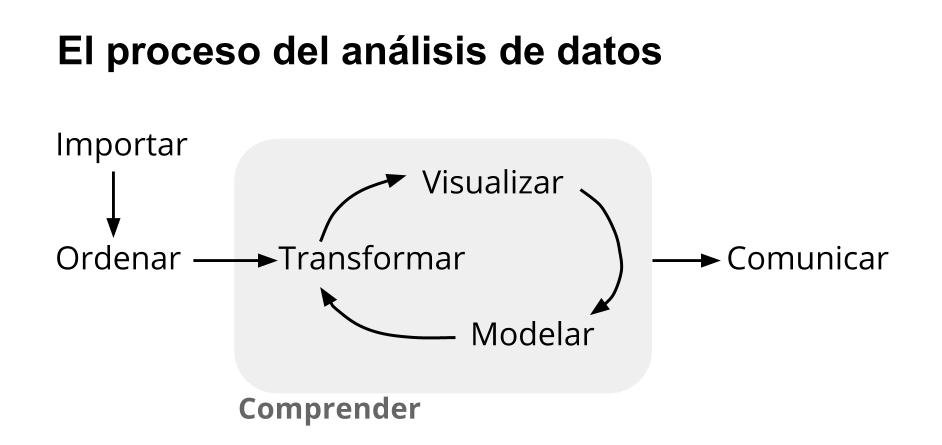
\includegraphics[width=6.28in]{imagenes/proceso_ciencia_datos} \caption{etapas en la aplicación de ciencia de datos}\label{fig:unnamed-chunk-3}
\end{figure}

Y todo ello llevado a cabo mediante la programación, por supuesto.

A lo largo de los capítulos de este libro vamos a aprender técnicas de
programación que nos permitan atravesar cada uno de los pasos del
proceso, y al hacerlo estaremos ejercitando las cuatro habilidades que
involucra la ciencia de datos.

Allá vamos.

\chapter{Una presentación a toda marcha de
R}\label{una-presentacion-a-toda-marcha-de-r}

\texttt{R} es un lenguaje de programación especializado en análisis y
visualización de datos. Es un producto de código abierto, lo cual
significa que cualquier persona puede usarlo y modificarlo sin pagar
licencias ni costos de adquisición de ningún tipo.

Expertos de todo el mundo colaboran en forma activa con el proyecto, no
sólo desarrollando el lenguaje en sí (llamado ``R base''), sino también
extendiéndolo con nuevas habilidades que pueden ser incorporadas por los
usuarios finales en forma de ``paquetes'' de funciones que pueden ser
instaladas.

La calidad del lenguaje en sí, de los paquetes instalables que le
agregan un sinfín de funciones (desde algoritmos de inteligencia
artificial hasta la generación de mapas interactivos) y de la comunidad
de usuarios que comparte información en foros y blogs, ha hecho de R uno
de los lenguajes de programación más populares del mundo. En el campo
del análisis de datos, es la herramienta por excelencia en muchas
universidades, empresas de tecnología, y redacciones de periodismo de
datos.

\section{Nuestro primer proyecto en
R}\label{nuestro-primer-proyecto-en-r}

A continuación reproduciremos un ejercicio paso a paso, para ilustrar la
potencia de una herramienta de análisis como R. Que nadie se preocupe si
algunas de las operaciones parecen no tener sentido, o resultan
arbitrarias. ¡Es normal! Nadie aprende un lenguaje en 10 minutos, sea R
o esperanto. La idea es tener exposición temprana a un caso de uso
interesante, usando datos reales. Y que nos sirva como motivación para
practicar luego ejercicios básicos que son muy necesarios pero, a veces,
no tan emocionantes.

\subsection{A investigar: ¿Cual es la diferencia en mortalidad infantil
entre el sur y el norte de la Ciudad Autónoma de Buenos
Aires?}\label{a-investigar-cual-es-la-diferencia-en-mortalidad-infantil-entre-el-sur-y-el-norte-de-la-ciudad-autonoma-de-buenos-aires}

Buenos Aires es una ciudad que desde hace décadas presenta una
\href{https://elpais.com/internacional/2016/10/16/argentina/1476629610_416732.html}{marcada
polarización} entre sus barrios del sur, relativamente menos
desarrollados, y los del norte donde el nivel socioeconómico y la
calidad de vida son mayores.

\begin{figure}

\includegraphics[width=6.78in]{imagenes/noticia_caba} \caption{Artículo en la edición online de El País}\label{fig:unnamed-chunk-4}
\end{figure}

Uno de los aspectos más lamentables de la disparidad norte-sur, y sin
duda de los que más polémica y acusaciones cruzadas ha generado, es la
diferencia en la tasa de mortalidad infantil de acuerdo a la región de
la ciudad.

¿Qué tan grande es esa diferencia? ¿Cómo se distribuye geográficamente?

Vamos a utilizar R para responder esas preguntas y visualizar los
resultados de nuestro análisis, utilizando como fuente cifras oficiales
publicada por la ciudad.

\subsection{Crear un proyecto en
RStudio}\label{crear-un-proyecto-en-rstudio}

El primer paso es ejecutar RStudio, que ya deberíamos tener disponible
en nuestro sistema.

Una vez abierta la interfaz gráfica, creamos un proyecto nuevo,
cliqueando en
\texttt{File\ -\textgreater{}\ New\ Project...\ -\textgreater{}\ New\ Directory\ -\textgreater{}\ \ New\ Project}.
En la ventana que surge, elegir un nombre para el proyecto (por ejemplo,
``Practicando R'') y finalizar la operación cliqueando en
\texttt{Create\ project}.

Utilizar proyectos nos permite continuar otro día desde donde dejamos la
tarea al terminar una sesión. Es sólo cuestión de recuperar el proyecto
deseado la próxima vez que abrimos RStudio, cliqueando en
\texttt{File\ -\textgreater{}\ Recent\ Projects\ -\textgreater{}\ "nombre\ de\ mi\ proyecto"}.

Por ahora, sigamos trabajando. Vamos a crear un ``script''. Un script,
como su nombre en inglés lo indica, es un guión; una serie de pasos que
escribimos para que nuestra computadora ejecute en secuencia. Cliqueamos
en
\texttt{File\ -\textgreater{}\ New\ File\ -\textgreater{}\ R\ Script}.
De inmediato se abre una ventana con un editor de texto. ¡Ahora empieza
la acción!

\subsection{Escribiendo un script}\label{escribiendo-un-script}

Aprovechemos para dar un nombre a los áreas que vemos en RStudio:

\begin{figure}
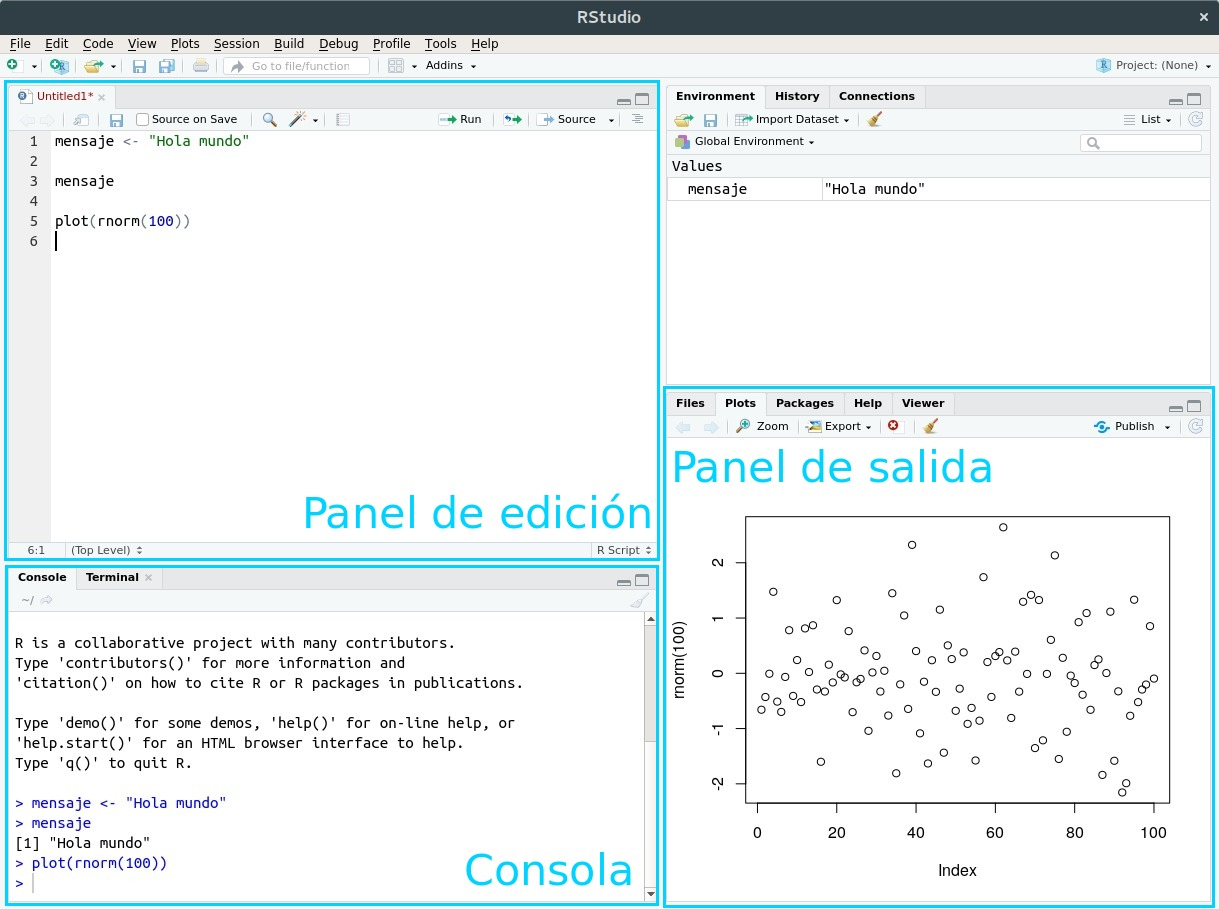
\includegraphics[width=8.13in]{imagenes/Interfaz_RStudio} \caption{La interfaz de RStudio}\label{fig:unnamed-chunk-5}
\end{figure}

Vamos a escribir nuestro código (las instrucciones que \texttt{R}
entiende) en el panel de edición. Los resultados van a aparecer en la
consola (cuando se trate de texto) o en el panel de salida (cuando
produzcamos gráficos)

Por ejemplo, podemos escribir el panel de edición la instrucción para
mostrar el resultado de una operación matemático:

\begin{Shaded}
\begin{Highlighting}[]
\KeywordTok{sqrt}\NormalTok{(}\DecValTok{144}\NormalTok{)}
\end{Highlighting}
\end{Shaded}

\texttt{sqrt()} es una \emph{función}. En el mundo de la programación,
las funciones son secuencias de código ya listas para usar, que realizan
tareas útiles. Por ejemplo, mostrar algo en pantalla. En nuestro caso,
completamos la función con algo más: un \emph{parámetro}, pues así se le
llama a los valores que una función espera de parte del usuario para
saber que hacer. La función print espera que le demos un número para el
cual calcular su raíz cuadrada (\emph{square root} en inglés), y eso
hicimos: le pasamos cómo parámetro \texttt{144}, un número. Los
parámetros siempre se escriben entre paréntesis, a continuación del
nombre de la función.

Ahora vamos a aprender la combinación de teclas más importante al usar
RStudio: \texttt{Ctrl} + \texttt{Enter}. Presionar \texttt{Ctrl} +
\texttt{Enter} al terminar de escribir una instrucción hace que RStudio
la ejecute de inmediato, y espere en la siguiente instrucción, si la
hubiera.

Cambien podemos buscar una línea que deseemos ejecutar, posicionando el
cursor de texto (que luce como una barra vertical que titila, en el
panel de edición) sobre ella. Si a continuación pulsamos \texttt{Ctrl} +
\texttt{Enter}, la línea será ejecutada y el cursor se moverá sólo hasta
la siguiente línea, listo para repetir el proceso.

La modalidad de ejecución línea por línea es muy útil para lo que se
llama ``análisis interactivo''. Uno ejecuta un comando, observa el
resultado, y en base a eso decide su próxima acción: cambiar parámetros
e intentarlo de nuevo, dar por buenos los resultados y usarlos para una
tarea subsiguiente\ldots{} etc.

Por ejemplo, si escribimos las siguientes líneas:

\begin{Shaded}
\begin{Highlighting}[]
\KeywordTok{sqrt}\NormalTok{(}\DecValTok{144}\NormalTok{)}

\NormalTok{mensaje <-}\StringTok{ "Hola mundo"}

\NormalTok{mensaje}
\end{Highlighting}
\end{Shaded}

\ldots{}y posicionamos el cursor en cualquier posición de la primera
línea, para luego pulsar \texttt{Ctrl} + \texttt{Enter} tres veces,
veremos que las instrucciones son ejecutadas línea a línea.

\begin{Shaded}
\begin{Highlighting}[]
\KeywordTok{sqrt}\NormalTok{(}\DecValTok{144}\NormalTok{)}
\end{Highlighting}
\end{Shaded}

\begin{verbatim}
## [1] 12
\end{verbatim}

\begin{Shaded}
\begin{Highlighting}[]
\NormalTok{mensaje <-}\StringTok{ "Hola mundo"}
\end{Highlighting}
\end{Shaded}

\begin{Shaded}
\begin{Highlighting}[]
\NormalTok{mensaje}
\end{Highlighting}
\end{Shaded}

\begin{verbatim}
## [1] "Hola mundo"
\end{verbatim}

Dos de ellas (la primera y la última) mostraron una salida en pantalla,
y la del medio, no. Esto es porque algunas funciones entregan algo como
resultado algo -un número, un texto, un gráfico, u otros tipos de salida
que ya veremos- mientras que otras hacen su tarea silenciosamente sin
expresar nada. En este caso, la función silenciosa fue la de asignación:
\texttt{mensaje\ \textless{}-\ "Hola\ mundo"} es una instrucción que le
pide a R que cree una variable llamada ``mensaje'' (o que la encuentre
si ya existe) y que le asigne como valor el texto ``Hola mundo''. ¿Cómo
sabemos que la instrucción se llevó a cabo, a pesar de no producir una
salida? En general, es un tema de confianza. Si una instrucción no
genera un mensaje de error, si es silenciosa, se asume que pudo cumplir
su cometido. En este caso, además lo hemos verificado. La línea final,
\texttt{mensaje} pide a R que busque la variable, y muestre en pantalla
su contenido (esa es una característica muy práctica del lenguaje: para
saber el contenido de una variable, basta con escribirla y ejecutar la
línea). Y al hacerlo, comprobamos que la variable contiene precisamente
lo que hemos tipeado.

De paso, hay que mencionar que la creación y manipulación de variables
es un concepto clave en programación. Trabajar con variables nos permite
almacenar valores para usarlos después, además de hacer nuestro código
más fácil de leer y compartir con otros, en especial cuando usamos
nombre de variable auto-explicativos. Como ejemplo de ésto ultimo
comparemos

\begin{Shaded}
\begin{Highlighting}[]
\NormalTok{x <-}\StringTok{ }\DecValTok{8} \OperatorTok{*}\StringTok{ }\DecValTok{6}
\NormalTok{x}
\end{Highlighting}
\end{Shaded}

\begin{verbatim}
## [1] 48
\end{verbatim}

\ldots{} con

\begin{Shaded}
\begin{Highlighting}[]
\NormalTok{ancho_habitacion_m <-}\StringTok{ }\DecValTok{8}
\NormalTok{profundiad_habitacion_m <-}\StringTok{ }\DecValTok{6}
\NormalTok{superficie_habitacion_m2 <-}\StringTok{ }\NormalTok{ancho_habitacion_m }\OperatorTok{*}\StringTok{ }\NormalTok{profundiad_habitacion_m}

\NormalTok{superficie_habitacion_m2}
\end{Highlighting}
\end{Shaded}

\begin{verbatim}
## [1] 48
\end{verbatim}

En su resultado ambas expresiones son iguales, dado que producen lo
mismo. Pero la segunda esta escrita de una forma mucho más clara para un
ser humano, que hace más fácil interpretar su lógica\ldots{} ¡está
calculando la superficie en metros cuadrados de una habitación!. Es muy
importante escribir nuestro código de la forma más explícita posible,
aunque requiera tipear un poco más. Con ello, le hacemos la vida más
fácil a otras personas que interpreten nuestros programas. Y también a
nosotros mismos en el futuro, cuando debamos lidiar con un programa que
escribimos tiempo atrás y del que a duras penas recordamos su lógica.

A todo esto\ldots{} ¿no se suponía que íbamos a investigar la mortalidad
infantil en la Ciudad de Buenos Aires?. Suficiente introducción\ldots{}
¡allá vamos!

\subsection{Cargar los datos}\label{cargar-los-datos}

Vamos a cargar datos de mortalidad infantil, por comuna de la ciudad, en
el año 2016, publicados por la
\href{http://www.estadisticaciudad.gob.ar/eyc/?p=67358}{Dirección
General de Estadística y Censos} de Buenos Aires. El formato original de
los datos es ``.xls'' (planilla de hojas de cálculo). Yo lo he
convertido a .csv (``comma separated values'') un formato muy popular en
el mundo de la ciencia de datos, ya que es muy fácil de manipular y
compartir entre sistemas\ldots{} es posible abrir un archivo .csv hasta
con el \href{https://es.wikipedia.org/wiki/Bloc_de_notas}{humilde block
de notas}. Al igual que los archivos .xls, los .csv se utilizan para
guardar información tabular: un rectángulo con filas y columnas. R
incluye una función que lee archivos .csv, que se llama
\texttt{read.csv}. La usamos así:

\begin{Shaded}
\begin{Highlighting}[]
\NormalTok{mortalidad <-}\StringTok{ }\KeywordTok{read.csv}\NormalTok{(}\StringTok{'https://bitsandbricks.github.io/data/mortalidad_infantil_caba_2016.csv'}\NormalTok{)}
\end{Highlighting}
\end{Shaded}

Obsérvese que los datos están alojados en un servidor de internet
(accesibles vía \textbf{\url{https://bitsandbricks}\ldots{}}). Eso no es
problema para la función read.csv, que con la misma soltura lee archivos
guardados en nuestra PC o publicados en un sitio web. Para ver el
contenido de la variable donde guardamos el resultado de leer la data,
\texttt{mortalidad}, sólo hace falta escribir su nombre:

\begin{Shaded}
\begin{Highlighting}[]
\NormalTok{mortalidad}
\end{Highlighting}
\end{Shaded}

\begin{verbatim}
##    Comuna Tasa2016
## 1       1      9.5
## 2       2      3.6
## 3       3      8.0
## 4       4     11.9
## 5       5      8.5
## 6       6      2.4
## 7       7      8.5
## 8       8      9.7
## 9       9     10.1
## 10     10      3.6
## 11     11      6.2
## 12     12      7.1
## 13     13      4.5
## 14     14      3.2
## 15     15      6.4
\end{verbatim}

Vemos que la tabla tiene 15 columnas (una por
\href{https://es.wikipedia.org/wiki/Comunas_de_la_ciudad_de_Buenos_Aires}{cada
comuna de la ciudad}) y 7 columnas (una que indica la comuna, y 6 con
los valores de mortalidad para cada año entre 2010 y 2017).

En R, las tablas son llamadas \texttt{dataframes}. El dataframe es el
objeto por excelencia del análisis de datos. En concepto, es muy similar
a una tabla de excel; al fin y al cabo, ambos formatos guardan
información en celdas identificadas por fila y columna.

Algunas funciones útiles para explorar un dataframe que no conocemos son
\texttt{dim()}, que nos da las dimensiones del dataframe (cantidad de
filas y columnas), \texttt{names()} que nos dice como se llaman sus
columnas (que en general representan variables), y \texttt{head()} que
nos permite echar un vistazo rápido al contenido, mostrando sólo las
seis primeras filas (ésto es útil porque con frecuencia trabajamos con
dataframes que contienen miles o millones de filas, con lo que no tiene
sentido tratar de volcar todas en pantalla).

\begin{Shaded}
\begin{Highlighting}[]
\KeywordTok{dim}\NormalTok{(mortalidad)}
\end{Highlighting}
\end{Shaded}

\begin{verbatim}
## [1] 15  2
\end{verbatim}

\begin{Shaded}
\begin{Highlighting}[]
\KeywordTok{names}\NormalTok{(mortalidad)}
\end{Highlighting}
\end{Shaded}

\begin{verbatim}
## [1] "Comuna"   "Tasa2016"
\end{verbatim}

\begin{Shaded}
\begin{Highlighting}[]
\KeywordTok{head}\NormalTok{(mortalidad)}
\end{Highlighting}
\end{Shaded}

\begin{verbatim}
##   Comuna Tasa2016
## 1      1      9.5
## 2      2      3.6
## 3      3      8.0
## 4      4     11.9
## 5      5      8.5
## 6      6      2.4
\end{verbatim}

\section{Visualización: la exploración gráfica de la
información}\label{visualizacion-la-exploracion-grafica-de-la-informacion}

Ahora es vamos a pisar el acelerador. Insisto: nadie debe preocuparse si
algunos conceptos parecen ser demasiado complejos. En las próximas
secciones practicaremos de forma gradual las técnicas que vamos a usar
ahora, y todo tendrá sentido -¡lo prometo!. Pero antes, seamos un
poquito irresponsables con el poder de R y empleemos un arsenal
sofisticado de herramientas para ver de que somos capaces.

En la introducción hablamos de los paquetes, conjuntos de programas que
extienden la funcionalidad de R. Vamos a cargar uno de los paquetes más
usados, \texttt{tidyverse}. Tidyverse incluye una gran cantidad de
funciones diseñadas por y para practicantes de la ciencia de datos.
Estas funciones comparten una filosofía y una sintaxis común, por lo que
al aprender una en cierto modo aprendemos a usar todas. El valor que
aportan es que, sin dudas, ayudan a realizar de manera más fácil las
tareas típicas de la ciencia de datos: importar, limpiar, comprender y
comunicar datos.

Si acabamos de instalar R y RStudio, el paquete aún no estará disponible
en nuestro sistema. Para instalarlo, usamos la función
\texttt{install.packages()} y le pasamos el nombre del paquete deseado,
``tidyverse'', entre comillas. Los dos comandos siguientes, que también
debemos ejecutar, se aseguran de que dispongamos de ciertas funciones
del paquete que son ``experimentales'' (es decir, en fase de prueba)
pero que queremos agregar porque las vamos a usar en breve. La
instalación puede tomar unos minutos, así que tengamos paciencia.

\begin{Shaded}
\begin{Highlighting}[]
\KeywordTok{install.packages}\NormalTok{(}\StringTok{"tidyverse"}\NormalTok{)}

\KeywordTok{install.packages}\NormalTok{(}\StringTok{"devtools"}\NormalTok{)}
\NormalTok{devtools}\OperatorTok{::}\KeywordTok{install_github}\NormalTok{(}\StringTok{"tidyverse/ggplot2"}\NormalTok{, }\DataTypeTok{dependencies =} \OtherTok{FALSE}\NormalTok{)}
\end{Highlighting}
\end{Shaded}

De aquí en más, podremos activar el conjunto de funciones que provee
\texttt{tidyverse} cada vez que queramos. Para eso, lo invocamos con la
función \texttt{library()}:

\begin{Shaded}
\begin{Highlighting}[]
\KeywordTok{library}\NormalTok{(tidyverse)}
\end{Highlighting}
\end{Shaded}

\ldots{} y listo para usar. La razón por la cual activamos tidyverse es
que en este momento nos vienen bien dos de sus funciones:
\texttt{mutate()} para modificar valores, y \texttt{ggplot()} para hacer
gráficos.

Bien, llega la hora de los gráficos. Vamos a llamar a la función
\texttt{ggplot()}, una auténtica navaja suiza para la visualización.

Por ejemplo, veamos a cuanto asciende la tasa de mortalidad infantil en
cada comuna durante 2016:

\begin{Shaded}
\begin{Highlighting}[]
\KeywordTok{ggplot}\NormalTok{(mortalidad) }\OperatorTok{+}
\StringTok{    }\KeywordTok{geom_col}\NormalTok{(}\KeywordTok{aes}\NormalTok{(}\DataTypeTok{x =} \KeywordTok{factor}\NormalTok{(Comuna), }\DataTypeTok{y =}\NormalTok{ Tasa2016))}
\end{Highlighting}
\end{Shaded}

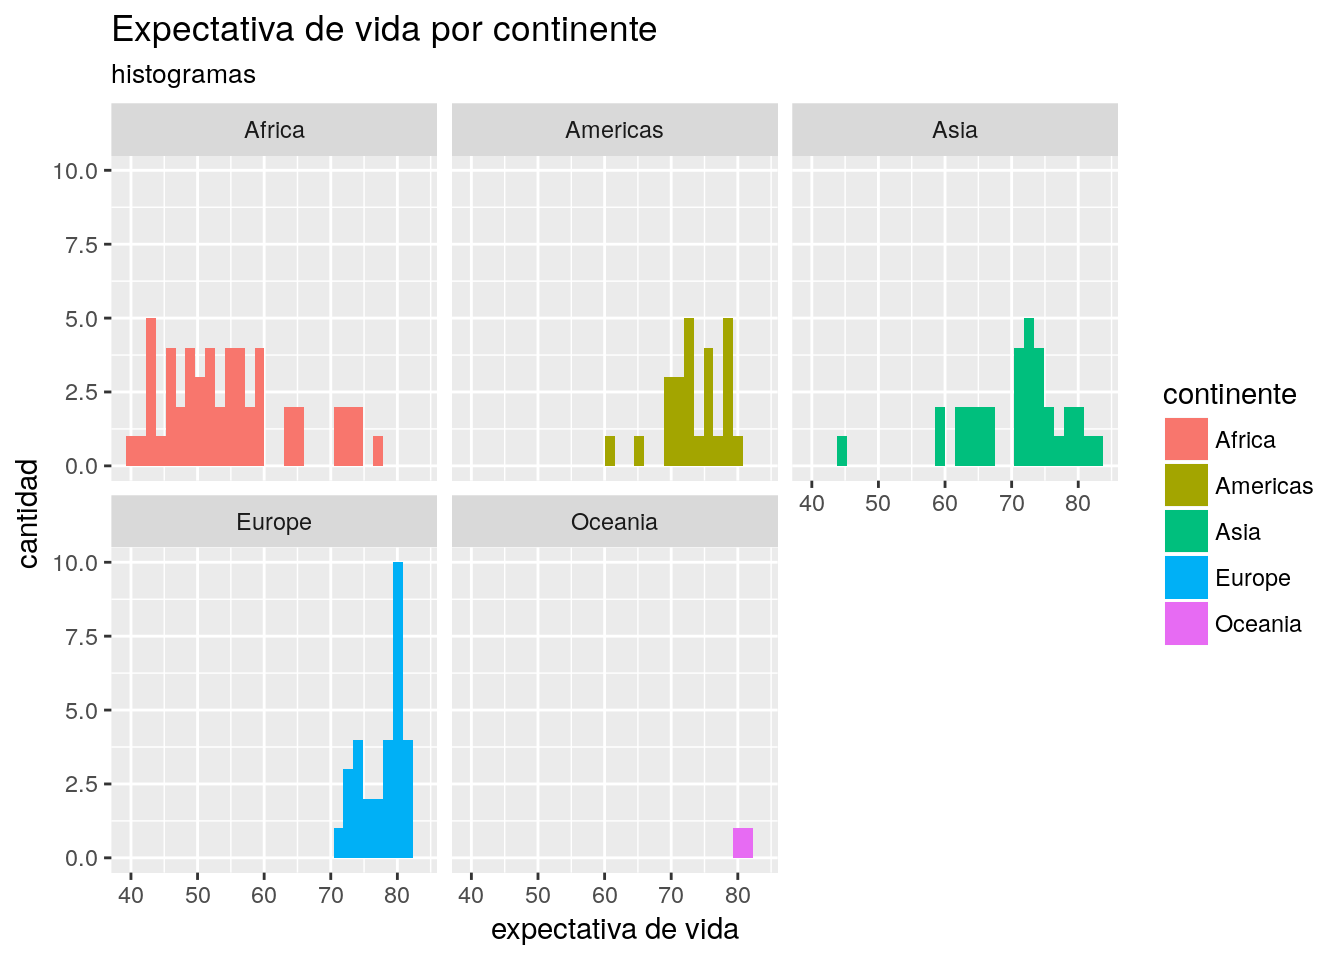
\includegraphics{ciencia_de_datos_para_gente_sociable_files/figure-latex/unnamed-chunk-18-1.pdf}

Para realizar una visualización con ésta herramienta, siempre se
comienza con la función ggplot(), que crea un eje de coordenadas sobre
el cual se pueden agregar capas. El primer parámetro que recibe ggplot()
es el dataset que queremos usar para el gráfico; en nuestro caso,
ggplot(mortalidad). Ejecutar sólo ggplot(mortalidad) nos devuelve un
gráfico vacío; la gracia está en agregar una o más capas especificando
cómo queremos mostrar los datos. Estas capas se agregan con un signo
\texttt{+}.

En nuestro ejemplo, \texttt{geom\_col()} crea columnas cuya posición en
el eje de las x depende de la variable ``Comuna'', mientas que la altura
(posición en el eje de las y) depende del valor de la variable
``Tasa2016''. Existen muchas funciones de tipo ``geom\_XXX'', que
agregan distintas clases de capas al gráfico: geom\_point,
geom\_polygon, geom\_text y muchos, muchos más que iremos viendo más
adelante.

Cada función ``geom\_'' toma como parámetro un conjunto de definiciones
``estéticas'' que le indican una variable a graficar (``mortalidad'' en
nuestro caso), cómo (color, tamaño, etc) y dónde (posición x, posición y
del eje). Estos parámetros van siempre dentro de una función auxiliar,
\texttt{aes()}. En nuestro ejemplo, ``geom\_line(aes(x = año, y =
mortalidad, group = Comuna, color = factor(Comuna)))''.

No se preocupen que iremos practicando el uso de ggplot, y su uso se
volverá familiar.

En cuanto al gráfico que hemos creado, podemos observar que entre las 15
comunas en la ciudad, la tasa de mortalidad tiene un rango que va de un
poco menos de 2,5 a un poco más de 12,5 (esto es, muertes antes del año
de vida por cada 10.000 nacimientos).

Pero no se distingue aquello que queríamos comprender: la diferencia
entre el norte y el sur de la ciudad. Necesitamos contexto geográfico.

\subsection{Haciendo mapas}\label{haciendo-mapas}

Vamos a presentar un paquete más, el último para éste capítulo:
\texttt{sf}. Quizás algunos tengan experiencia con sistemas de
información geográfica (GIS por sus siglas en inglés), al estilo de
\href{https://qgis.org/en/site/}{QGIS} o
\href{https://www.arcgis.com/features/index.html}{ArcGIS}, que permiten
crear, manipular y combinar archivos con datos espaciales para producir
mapas que pueden ser simples o en extremo sofisticados. En R, el paquete
\texttt{sf} brinda herramientas que permiten realizar tares similares.

Nuestro objetivo es obtener un mapa de la ciudad de Buenos Aires con sus
comunas.

Primero, instalamos sf en caso de que aún no lo hayamos hecho. Sólo es
necesario hacerlo una vez:

\begin{Shaded}
\begin{Highlighting}[]
\KeywordTok{install.packages}\NormalTok{(}\StringTok{"sf"}\NormalTok{)}
\end{Highlighting}
\end{Shaded}

Pedimos a R que active el paquete:

\begin{Shaded}
\begin{Highlighting}[]
\KeywordTok{library}\NormalTok{(sf)}
\end{Highlighting}
\end{Shaded}

Y cargamos un archivo georeferenciado con las comunas de la Ciudad
Autónoma de Buenos Aires, disponible online en formato
\href{https://es.wikipedia.org/wiki/GeoJSON}{\emph{geojson}}, un
estándar de representación de datos geográficos que es fácil de usar:

\begin{Shaded}
\begin{Highlighting}[]
\NormalTok{comunas <-}\StringTok{ }\KeywordTok{st_read}\NormalTok{(}\StringTok{'https://bitsandbricks.github.io/data/CABA_comunas.geojson'}\NormalTok{)}
\end{Highlighting}
\end{Shaded}

\begin{verbatim}
## Reading layer `CABA_comunas' from data source `https://bitsandbricks.github.io/data/CABA_comunas.geojson' using driver `GeoJSON'
## Simple feature collection with 15 features and 4 fields
## geometry type:  MULTIPOLYGON
## dimension:      XY
## bbox:           xmin: -58.53152 ymin: -34.70529 xmax: -58.33514 ymax: -34.52754
## epsg (SRID):    4326
## proj4string:    +proj=longlat +datum=WGS84 +no_defs
\end{verbatim}

Al igual que cuando usamos \texttt{read.csv()} para leer un archivo .csv
y cargarlo como un dataframe, el comando \texttt{st\_read()} hace lo
propio con archivos de información geográfica, conocidos en la jerga
como ``shapefiles''. El resultado también es un dataframe, por lo cual
podemos practicar el uso de las funciones que ya aprendimos, como dim(),
names() y head().

\begin{Shaded}
\begin{Highlighting}[]
\KeywordTok{dim}\NormalTok{(comunas)}
\end{Highlighting}
\end{Shaded}

\begin{verbatim}
## [1] 15  5
\end{verbatim}

\begin{Shaded}
\begin{Highlighting}[]
\KeywordTok{names}\NormalTok{(comunas)}
\end{Highlighting}
\end{Shaded}

\begin{verbatim}
## [1] "barrios"   "perimetro" "area"      "comunas"   "geometry"
\end{verbatim}

\begin{Shaded}
\begin{Highlighting}[]
\KeywordTok{head}\NormalTok{(comunas)}
\end{Highlighting}
\end{Shaded}

\begin{verbatim}
## Simple feature collection with 6 features and 4 fields
## geometry type:  MULTIPOLYGON
## dimension:      XY
## bbox:           xmin: -58.4627 ymin: -34.6625 xmax: -58.33514 ymax: -34.56935
## epsg (SRID):    4326
## proj4string:    +proj=longlat +datum=WGS84 +no_defs
##                                                                        barrios
## 1 CONSTITUCION - MONSERRAT - PUERTO MADERO -  RETIRO - SAN NICOLAS - SAN TELMO
## 2                                                                     RECOLETA
## 3                                                    BALVANERA - SAN CRISTOBAL
## 4                           BARRACAS - BOCA - NUEVA POMPEYA - PARQUE PATRICIOS
## 5                                                              ALMAGRO - BOEDO
## 6                                                                    CABALLITO
##   perimetro     area comunas                       geometry
## 1  35572.65 17802807       1 MULTIPOLYGON (((-58.36854 -...
## 2  21246.61  6140873       2 MULTIPOLYGON (((-58.39521 -...
## 3  10486.26  6385991       3 MULTIPOLYGON (((-58.41192 -...
## 4  36277.44 21701236       4 MULTIPOLYGON (((-58.3552 -3...
## 5  12323.47  6660526       5 MULTIPOLYGON (((-58.41287 -...
## 6  10990.96  6851029       6 MULTIPOLYGON (((-58.43061 -...
\end{verbatim}

Podemos ver que el dataframe contiene 15 filas y 5 columnas. Una fila
por comuna (es razonable!) y 5 columnas: ``barrios'', ``perímetro'',
``area'', ``comunas'' y ``geometry''. Nuestro vistazo mediante head()
permite asumir que ``barrios'' informa los barrios que componen cada
comuna, mientras que perímetro y área informan sobre las dimensiones del
polígono cubierto por cada comuna. La columna ``geometry'' aparece en
todos los dataframes de tipo espacial, y es la que contiene los datos
con sus coordenadas geográficas.

Y hablando de coordenadas, generar un mapa a partir de un dataframe
espacial creado por sf es muy fácil con la ayuda de ggplot

\begin{Shaded}
\begin{Highlighting}[]
\KeywordTok{ggplot}\NormalTok{(comunas) }\OperatorTok{+}
\StringTok{    }\KeywordTok{geom_sf}\NormalTok{()}
\end{Highlighting}
\end{Shaded}

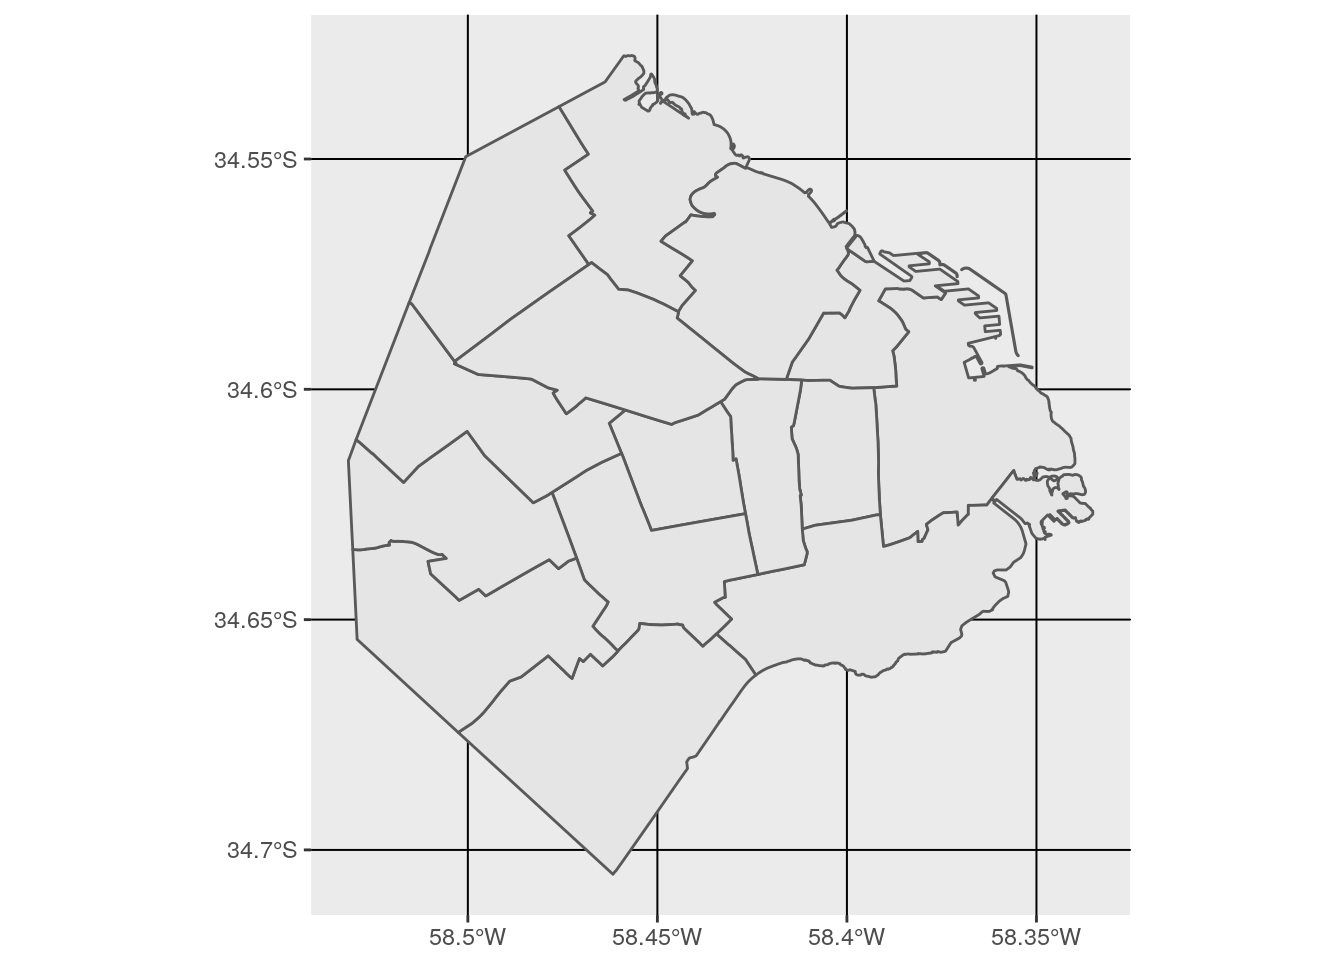
\includegraphics{ciencia_de_datos_para_gente_sociable_files/figure-latex/unnamed-chunk-23-1.pdf}

Si queremos agregar una leyenda al mapa que identifique cada comuna con
su número, usamos:

\begin{Shaded}
\begin{Highlighting}[]
\KeywordTok{ggplot}\NormalTok{(comunas) }\OperatorTok{+}
\StringTok{    }\KeywordTok{geom_sf}\NormalTok{(}\KeywordTok{aes}\NormalTok{(}\DataTypeTok{fill =}\NormalTok{ comunas))}
\end{Highlighting}
\end{Shaded}

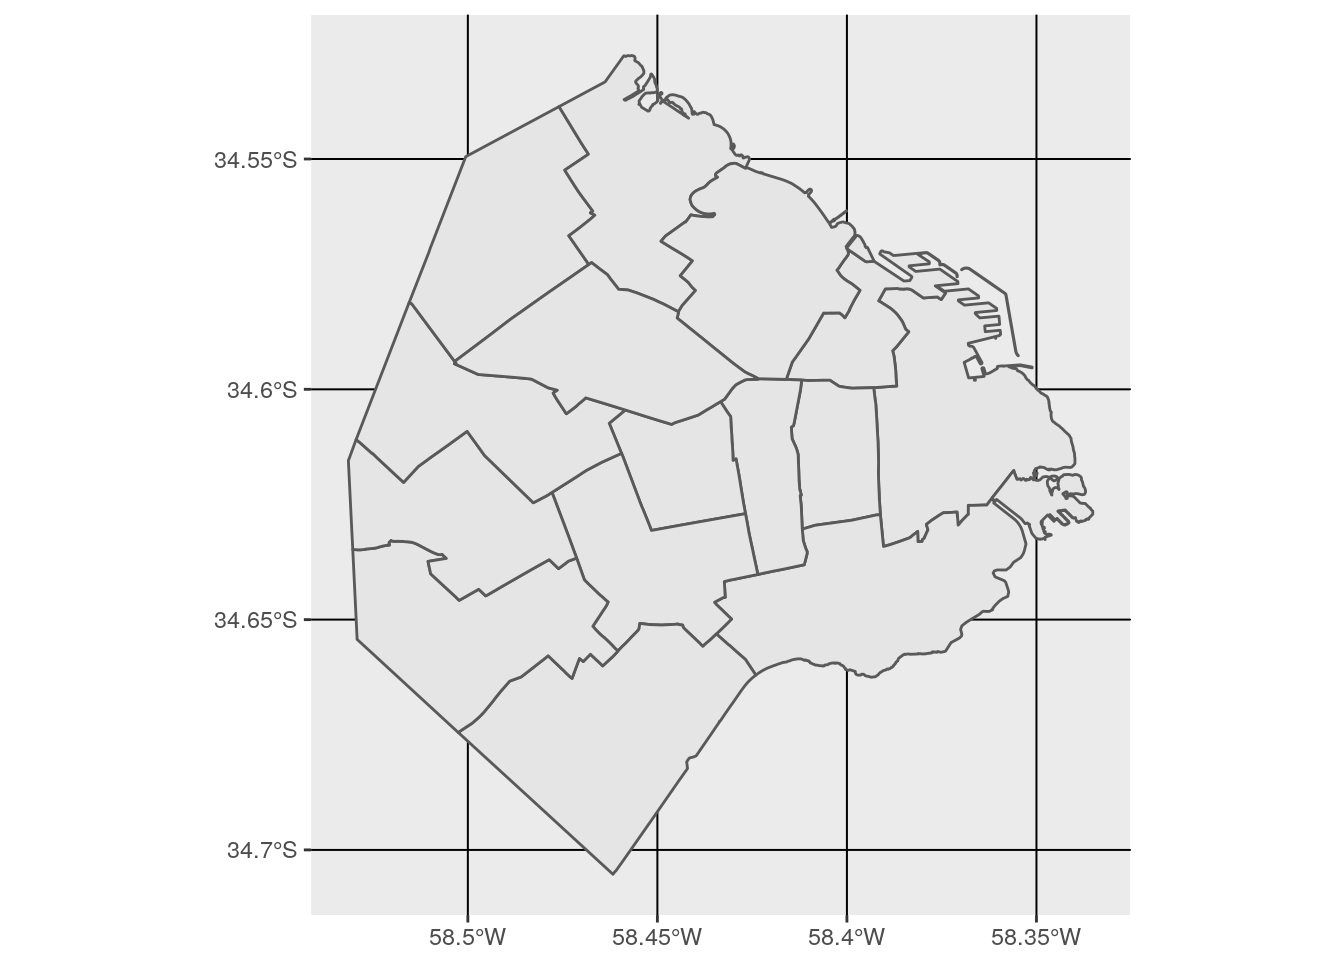
\includegraphics{ciencia_de_datos_para_gente_sociable_files/figure-latex/unnamed-chunk-24-1.pdf}

Dentro de ``aes()'' usé el parámetro ``fill'' (relleno en inglés) para
pedirle a ggplot que llene cada polígono con un color distinto de
acuerdo al campo ``comunas''.

Aprovechando que tenemos un mapa, deberíamos clasificar las comunas
entre las que pertenecen al norte y las que pertenecen al sur de la
ciudad. No hay una línea divisoria oficial, pero la traza de la Avenida
Rivadavia suele ser tomada como frontera: Rivadavia es la
\href{https://www.clarin.com/ediciones-anteriores/avenida-rivadaviaun-largo-recorrido-contrastes_0_B1reo181CYe.html}{``divisoria
simbólica del Norte y el Sur de la Ciudad, con sus diferencias de
desarrollo''}

Por esas casualidades de la vida, tengo un archivo geográfico que
contiene la línea que dibuja a avenida Rivadavia al atravesar la ciudad.
Lo bajamos:

\begin{Shaded}
\begin{Highlighting}[]
\NormalTok{rivadavia <-}\StringTok{ }\KeywordTok{st_read}\NormalTok{(}\StringTok{'https://bitsandbricks.github.io/data/avenida_rivadavia.geojson'}\NormalTok{)}
\end{Highlighting}
\end{Shaded}

\begin{verbatim}
## Reading layer `avenida_rivadavia' from data source `https://bitsandbricks.github.io/data/avenida_rivadavia.geojson' using driver `GeoJSON'
## Simple feature collection with 1 feature and 1 field
## geometry type:  LINESTRING
## dimension:      XY
## bbox:           xmin: -58.53014 ymin: -34.63946 xmax: -58.37017 ymax: -34.60711
## epsg (SRID):    4326
## proj4string:    +proj=longlat +datum=WGS84 +no_defs
\end{verbatim}

Y lo proyectamos sobre el mapa, como una capa adicional del gráfico de
ggplot que definimos antes:

\begin{Shaded}
\begin{Highlighting}[]
\KeywordTok{ggplot}\NormalTok{(comunas) }\OperatorTok{+}
\StringTok{    }\KeywordTok{geom_sf}\NormalTok{(}\KeywordTok{aes}\NormalTok{(}\DataTypeTok{fill =}\NormalTok{ comunas)) }\OperatorTok{+}
\StringTok{    }\KeywordTok{geom_sf}\NormalTok{(}\DataTypeTok{data =}\NormalTok{ rivadavia, }\DataTypeTok{color =} \StringTok{"red"}\NormalTok{)}
\end{Highlighting}
\end{Shaded}

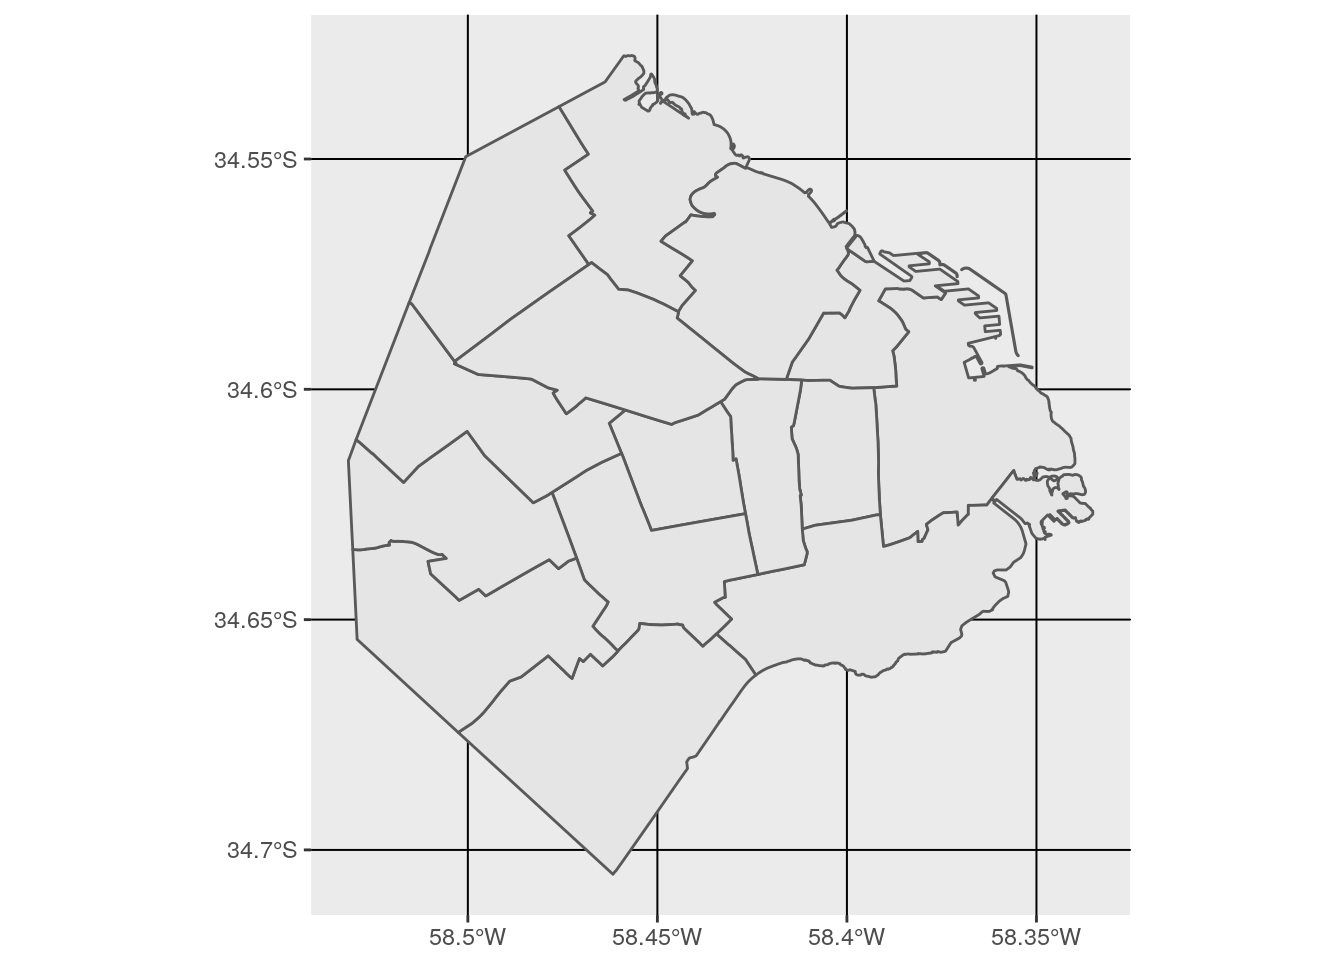
\includegraphics{ciencia_de_datos_para_gente_sociable_files/figure-latex/unnamed-chunk-26-1.pdf}

La identificación por colores no hace fácil reconocer con rapidez que
número corresponde a cada comuna; es un recurso que funciona mejor con
menos categorías que nuestras 15. Podríamos arreglarlo, por ejemplo
evitando la codificación por color, y dibujando una etiqueta con número
dibujada sobre cada comuna. ¡Pero no en este momento! En aras de la
sencillez, vamos a aguzar la vista y tomar nota de cuales comunas tienen
gran parte de su territorio al sur de la Avenida Rivadavia. Según mi
interpretación, son las comunas 1, 3, 4, 5, 7, 8 y 9. (Hay que admitir
que la comuna 1 parece estar repartida en partes más o menos iguales,
pero vamos a dejársela al sur en forma arbitraria para no complicar el
ejercicio).

\subsection{Agregando datos}\label{agregando-datos}

En este punto necesitamos una manera de ``etiquetar'' cada comuna con el
punto cardinal que le toca ``Norte'' o ``Sur''. La forma más rápida es
crear una lista con los atributos, y agregarla a nuestro dataframe como
una nueva columna.

Podemos armar una sucesión de 15 ``etiquetas'' según el punto cardinal
que le toca a cada comuna. El comando en R que ``une'' valores en
conjunto se llama \texttt{c()} (viene de ``combine'', ``combinar''), y
permite definir una lista de valores. Mejor dicho, un ``vector'' de
valores; en el mundo de la programación, se usa la palabra vector cuando
se combinan elementos del mismo tipo, y ``lista'' cuando se combina una
variedad de clases: en el mismo conjunto números, textos, y otros tipos
de objeto más complejos. Por ahora, no nos preocupemos por eso.

\begin{Shaded}
\begin{Highlighting}[]
\NormalTok{nueva_columna <-}\StringTok{ }\KeywordTok{c}\NormalTok{(}\StringTok{"Sur"}\NormalTok{, }\StringTok{"Norte"}\NormalTok{, }\StringTok{"Sur"}\NormalTok{, }\StringTok{"Sur"}\NormalTok{, }\StringTok{"Sur"}\NormalTok{, }\StringTok{"Norte"}\NormalTok{, }\StringTok{"Sur"}\NormalTok{, }\StringTok{"Sur"}\NormalTok{, }\StringTok{"Sur"}\NormalTok{, }\StringTok{"Norte"}\NormalTok{, }\StringTok{"Norte"}\NormalTok{, }\StringTok{"Norte"}\NormalTok{, }\StringTok{"Norte"}\NormalTok{, }\StringTok{"Norte"}\NormalTok{, }\StringTok{"Norte"}\NormalTok{)}

\NormalTok{nueva_columna}
\end{Highlighting}
\end{Shaded}

\begin{verbatim}
##  [1] "Sur"   "Norte" "Sur"   "Sur"   "Sur"   "Norte" "Sur"   "Sur"  
##  [9] "Sur"   "Norte" "Norte" "Norte" "Norte" "Norte" "Norte"
\end{verbatim}

Ya podemos agregar nuestra nueva columna usando una función que ya
vimos, mutate(). En el dataframe, vamos a ponerle a nuestra nueva
columna un nombre descriptivo, ``ubicación'' :

\begin{Shaded}
\begin{Highlighting}[]
\NormalTok{comunas <-}\StringTok{ }\KeywordTok{mutate}\NormalTok{(comunas, }\DataTypeTok{ubicacion =}\NormalTok{ nueva_columna)}
\end{Highlighting}
\end{Shaded}

Verifiquemos el resultado:

\begin{Shaded}
\begin{Highlighting}[]
\KeywordTok{head}\NormalTok{(comunas)}
\end{Highlighting}
\end{Shaded}

\begin{verbatim}
## Simple feature collection with 6 features and 5 fields
## geometry type:  MULTIPOLYGON
## dimension:      XY
## bbox:           xmin: -58.4627 ymin: -34.6625 xmax: -58.33514 ymax: -34.56935
## epsg (SRID):    4326
## proj4string:    +proj=longlat +datum=WGS84 +no_defs
##                                                                        barrios
## 1 CONSTITUCION - MONSERRAT - PUERTO MADERO -  RETIRO - SAN NICOLAS - SAN TELMO
## 2                                                                     RECOLETA
## 3                                                    BALVANERA - SAN CRISTOBAL
## 4                           BARRACAS - BOCA - NUEVA POMPEYA - PARQUE PATRICIOS
## 5                                                              ALMAGRO - BOEDO
## 6                                                                    CABALLITO
##   perimetro     area comunas ubicacion                       geometry
## 1  35572.65 17802807       1       Sur MULTIPOLYGON (((-58.36854 -...
## 2  21246.61  6140873       2     Norte MULTIPOLYGON (((-58.39521 -...
## 3  10486.26  6385991       3       Sur MULTIPOLYGON (((-58.41192 -...
## 4  36277.44 21701236       4       Sur MULTIPOLYGON (((-58.3552 -3...
## 5  12323.47  6660526       5       Sur MULTIPOLYGON (((-58.41287 -...
## 6  10990.96  6851029       6     Norte MULTIPOLYGON (((-58.43061 -...
\end{verbatim}

Y en el mapa:

\begin{Shaded}
\begin{Highlighting}[]
\KeywordTok{ggplot}\NormalTok{(comunas) }\OperatorTok{+}
\StringTok{    }\KeywordTok{geom_sf}\NormalTok{(}\KeywordTok{aes}\NormalTok{(}\DataTypeTok{fill =}\NormalTok{ ubicacion)) }\OperatorTok{+}
\StringTok{    }\KeywordTok{geom_sf}\NormalTok{(}\DataTypeTok{data =}\NormalTok{ rivadavia, }\DataTypeTok{color =} \StringTok{"red"}\NormalTok{)}
\end{Highlighting}
\end{Shaded}

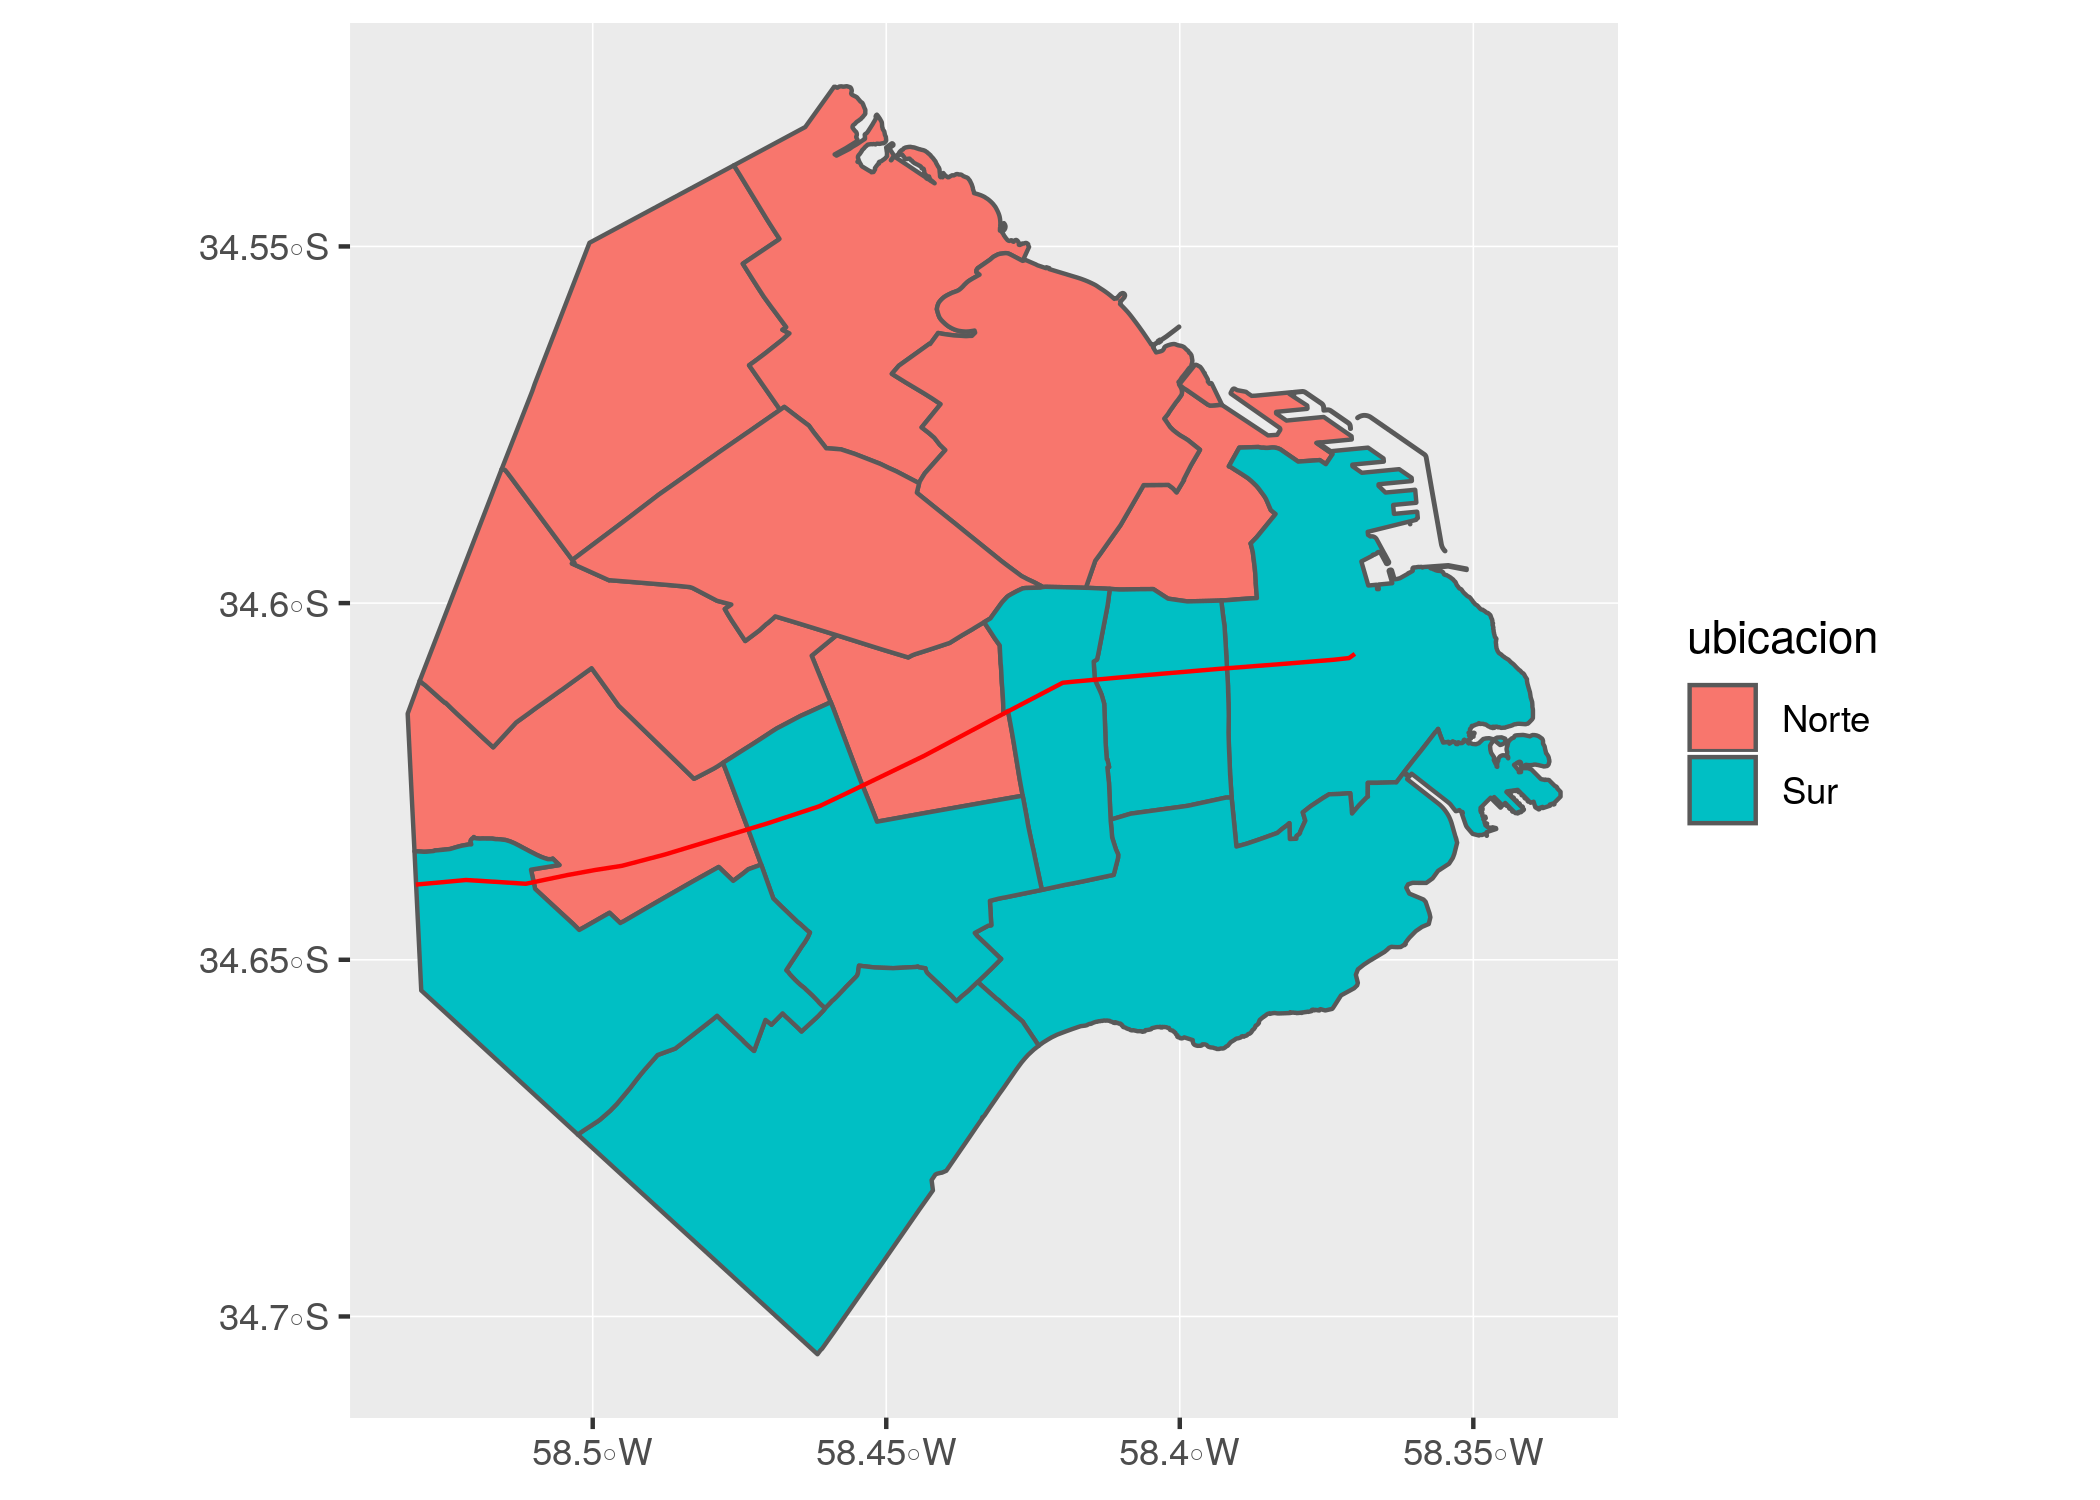
\includegraphics{ciencia_de_datos_para_gente_sociable_files/figure-latex/unnamed-chunk-30-1.pdf}

Todo en orden. Ahora hagamos lo mismo con el dataframe de mortalidad,
aprovechando que lista las comunas en el mismo orden (del 1 al 15) y por
lo tanto podemos ``pegarle'' el mismo vector de etiquetas con ubicación
que ya preparamos.

\begin{Shaded}
\begin{Highlighting}[]
\NormalTok{mortalidad <-}\StringTok{ }\KeywordTok{mutate}\NormalTok{(mortalidad, ubicación =}\StringTok{ }\NormalTok{nueva_columna)}
                         
\KeywordTok{head}\NormalTok{(mortalidad)}
\end{Highlighting}
\end{Shaded}

\begin{verbatim}
##   Comuna Tasa2016 ubicación
## 1      1      9.5       Sur
## 2      2      3.6     Norte
## 3      3      8.0       Sur
## 4      4     11.9       Sur
## 5      5      8.5       Sur
## 6      6      2.4     Norte
\end{verbatim}

\section{El veredicto final}\label{el-veredicto-final}

Habrán notado que llegar hasta aquí tomó una buena cantidad de
operaciones. En contraste, lo que estamos a punto de hacer -responder la
pregunta inicial- va a ser mucho más breve. Esa vendría a ser la lección
central de éste capítulo: la mayor parte del tiempo empleado en la labor
de la ciencia de datos se insume en la poco glamorosa tarea de
recopilar, limpiar y combinar los registros necesarios para el análisis.
Como consuelo, podemos pensar en que el esfuerzo necesario para llegar a
este punto nos ha dado un conocimiento de los datos (su estructura, sus
limitaciones, su potencial) que no teníamos antes.

Aprovechemos entonces nuestra data limpia y ordenada, para producir un
mapa que señale con color el nivel de mortalidad. Armamos un ggplot con
una capa que muestra las comunas, cuyo color interior (``fill'') depende
del valor de la mortalidad. Le sumamos una capa con la traza de la
Avenida Rivadavia, nuestra referencia de posición, y por último
definimos la paleta de colores a usar en el \emph{fill}, eligiendo una
llamada ``Spectral'', que va del azul al rojo y es muy usada cuando se
quiere resaltar la divergencia de una variable.

\begin{Shaded}
\begin{Highlighting}[]
\KeywordTok{ggplot}\NormalTok{(comunas) }\OperatorTok{+}
\StringTok{    }\KeywordTok{geom_sf}\NormalTok{(}\KeywordTok{aes}\NormalTok{(}\DataTypeTok{fill =}\NormalTok{ mortalidad}\OperatorTok{$}\NormalTok{Tasa2016)) }\OperatorTok{+}
\StringTok{    }\KeywordTok{geom_sf}\NormalTok{(}\DataTypeTok{data =}\NormalTok{ rivadavia, }\DataTypeTok{color =} \StringTok{"red"}\NormalTok{) }\OperatorTok{+}
\StringTok{    }\KeywordTok{scale_fill_distiller}\NormalTok{(}\DataTypeTok{palette =} \StringTok{"Spectral"}\NormalTok{)}
\end{Highlighting}
\end{Shaded}

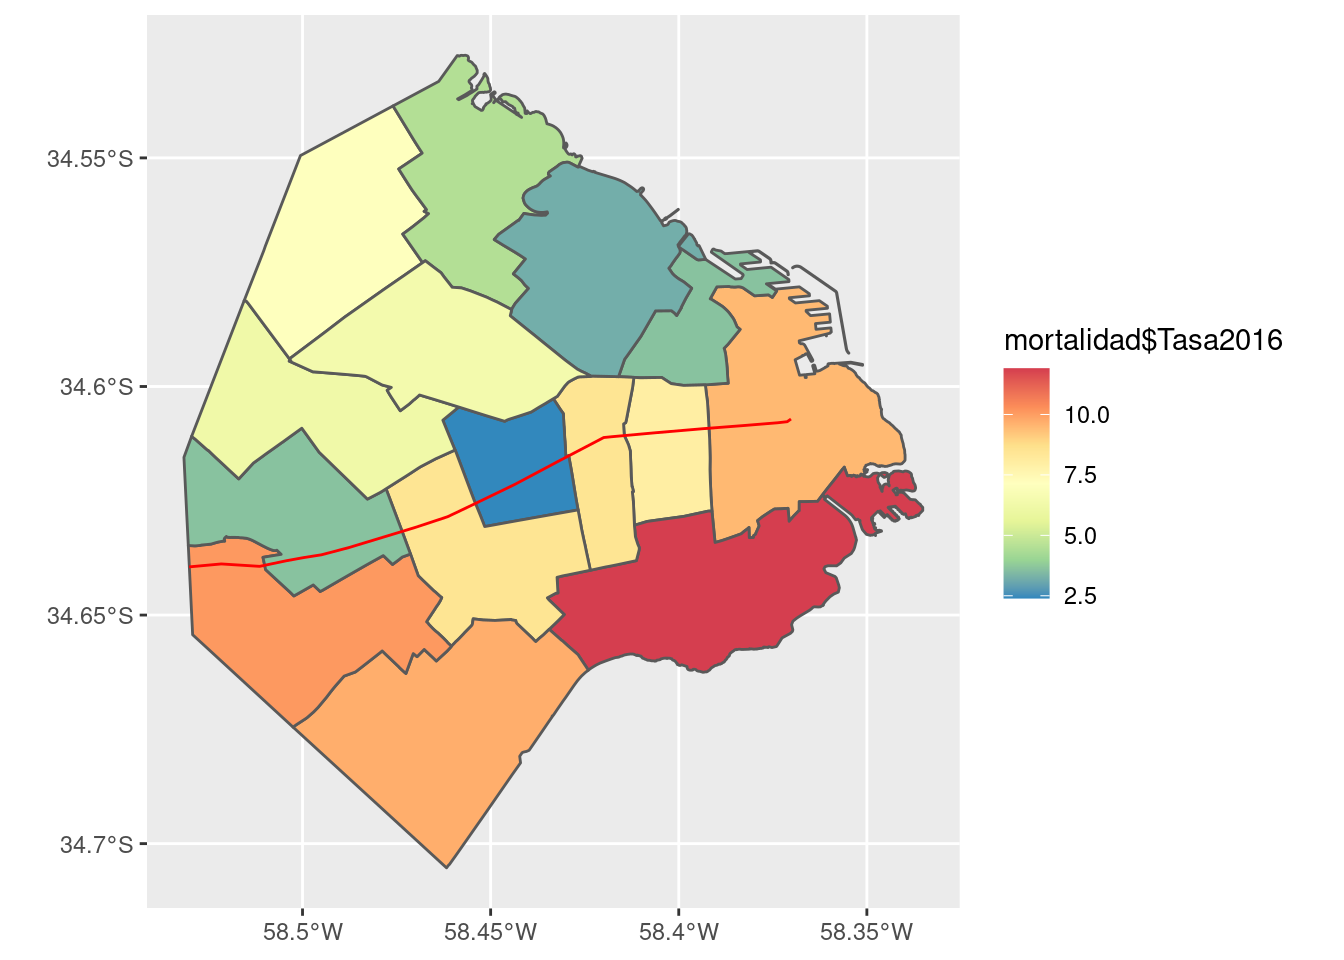
\includegraphics{ciencia_de_datos_para_gente_sociable_files/figure-latex/unnamed-chunk-32-1.pdf}

Para una comparación visual más precisa entre los valores de cada
comuna, le pedimos a ggplot un gráfico de barras, con la capa
\texttt{geom\_col()}. En las variables estéticas, definimos que la
posición de las barras en el eje de las x estará dada por el número de
cada comuna, la altura de las barras (eje y) será dada por su tasa de
mortalidad, y su color de relleno (fill) dependerá de su ubicación
geográfica.

\begin{Shaded}
\begin{Highlighting}[]
\KeywordTok{ggplot}\NormalTok{(mortalidad) }\OperatorTok{+}
\StringTok{    }\KeywordTok{geom_col}\NormalTok{(}\KeywordTok{aes}\NormalTok{(}\DataTypeTok{x =}\NormalTok{ Comuna, }\DataTypeTok{y =}\NormalTok{ Tasa2016, }\DataTypeTok{fill =}\NormalTok{ ubicación)) }\OperatorTok{+}
\StringTok{    }\KeywordTok{labs}\NormalTok{(}\DataTypeTok{title =} \StringTok{"Mortalidad infantil en la Ciudad Autónoma de Buenos Aires"}\NormalTok{,}
         \DataTypeTok{subtitle =} \StringTok{"Año 2016"}\NormalTok{,}
         \DataTypeTok{y =} \StringTok{"tasa"}\NormalTok{) }
\end{Highlighting}
\end{Shaded}

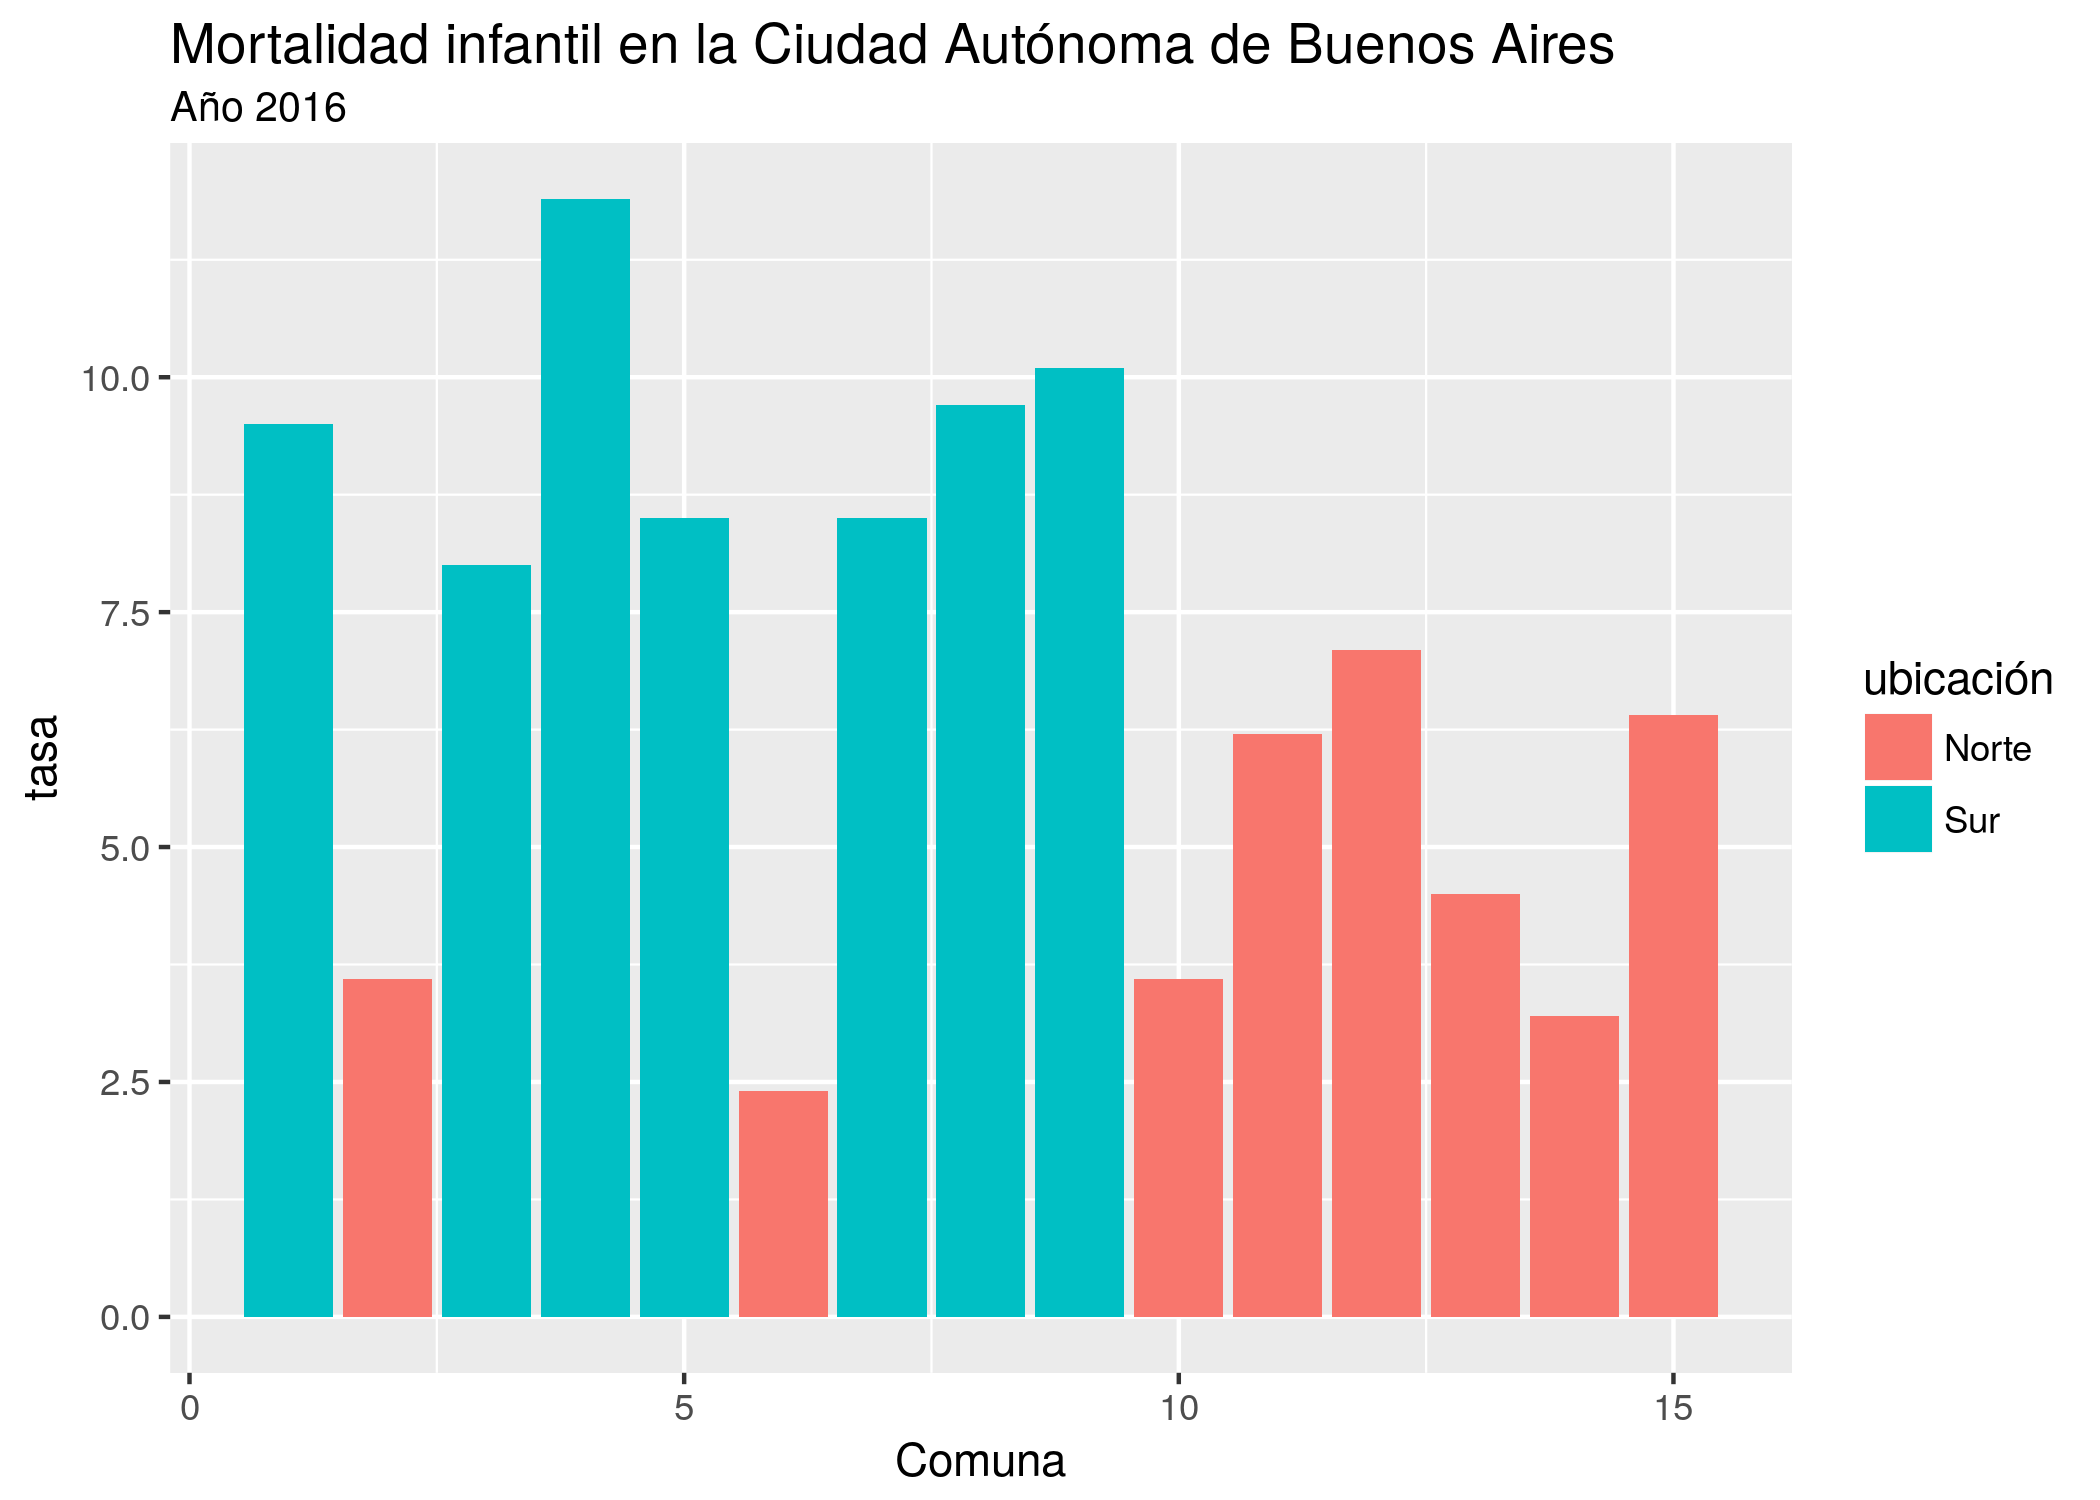
\includegraphics{ciencia_de_datos_para_gente_sociable_files/figure-latex/unnamed-chunk-33-1.pdf}

Por último, usamos a R de calculadora. Separamos las comunas en dos
dataframes distintos según su ubicación, con el comando
\texttt{filter()}\ldots{}

\begin{Shaded}
\begin{Highlighting}[]
\NormalTok{comunas_al_sur <-}\StringTok{ }\KeywordTok{filter}\NormalTok{(mortalidad, ubicación }\OperatorTok{==}\StringTok{ "Sur"}\NormalTok{)}

\NormalTok{comunas_al_norte <-}\StringTok{ }\KeywordTok{filter}\NormalTok{(mortalidad, ubicación }\OperatorTok{==}\StringTok{ "Norte"}\NormalTok{)}
\end{Highlighting}
\end{Shaded}

\ldots{} y calculamos la diferencia entre el promedio de mortalidad de
unas y otras.

\begin{Shaded}
\begin{Highlighting}[]
\KeywordTok{mean}\NormalTok{(comunas_al_sur}\OperatorTok{$}\NormalTok{Tasa2016) }\OperatorTok{/}\StringTok{ }\KeywordTok{mean}\NormalTok{(comunas_al_norte}\OperatorTok{$}\NormalTok{Tasa2016)}
\end{Highlighting}
\end{Shaded}

\begin{verbatim}
## [1] 2.044788
\end{verbatim}

\subsection{¿Cuál es la diferencia en mortalidad infantil entre el sur y
el norte de la Ciudad Autónoma de Buenos
Aires?}\label{cual-es-la-diferencia-en-mortalidad-infantil-entre-el-sur-y-el-norte-de-la-ciudad-autonoma-de-buenos-aires}

En base a lo que descubrimos, vamos a responder en forma sucinta.

\begin{itemize}
\item
  En el año 2016, la tasa de mortalidad infantil en todo los barrios del
  sur es más alta que en cualquier de los del norte.
\item
  Para los nacidos en 2016 de padres que viven en el sur de la ciudad,
  la posibilidad de morir antes del primer año es, en promedio, el doble
  que la de aquellos con padres que residen al norte.
\end{itemize}

Por supuesto, con esto no puede darse por cerrado el tema; hay muchas
facetas que deberíamos analizar para comenzar a entender un fenómeno
social de tal complejidad. Por ejemplo, ¿Cómo es la evolución en el
tiempo de la brecha norte/sur - se mantiene igual, decrece, aumenta?
¿Qué otros factores están correlacionados con la disparidad, más allá
del geográfico?

En los siguientes capítulos practicaremos varias técnicas que nos
permitirán profundizar nuestros análisis, en la nunca finalizada misión
de entender un poco más.

\chapter{Poniendo los datos en forma}\label{poniendo-los-datos-en-forma}

Cómo ya hemos mencionado, es normal que la mayor parte del tiempo
dedicado a un proyecto de análisis se nos vaya en la limpieza y orden de
los datos disponibles. Aún cuando nuestros datos provengan de fuentes
oficiales (un gobierno nacional, el Banco Mundial, etc) en muy rara
ocasión podremos usarlos para nuestros fines sin antes procesarlos. Y
aún si los datos llegaran en perfectas condiciones, no tenemos forma de
saberlo hasta haber realizado una exploración para verificarlo.

Ésta inevitable etapa de preparación es llamada \emph{data wrangling} en
inglés, algo así como el proceso de ``domar los datos''. El término hace
referencia, en clave de humor, al esfuerzo que requiere la puesta en
orden cuando los datos son cuantiosos, de muchas fuentes distintas, o en
particular desprolijos. Para que la experiencia sea lo menos tediosa
posible, y podamos pasar rápido al momento de extraer conocimiento,
vamos a practicar algunas técnicas muy útiles de \emph{wrangling}.

\section{Primeros pasos al examinar un conjunto de datos
nuevo}\label{primeros-pasos-al-examinar-un-conjunto-de-datos-nuevo}

Vamos a practicar usando los registros del Sistema Único de Atención
Ciudadana (SUACI) de la Ciudad Autónoma de Buenos Aires. El SUACI es el
repositorio donde se integran las solicitudes y reclamos que los
ciudadanos presentan a la ciudad por distintos canales: en persona, por
teléfono o usando la aplicación
\href{https://gestioncolaborativa.buenosaires.gob.ar/prestaciones}{BA
147}. Vamos a trabajar con una versión de los datos que ha sido
simplificada para hacer más ameno el trabajo con ella. Quién quiera
acceder a los datos en su esplendor de complejidad original, puede
encontrarlos en el portal de datos abiertos de la ciudad:
\url{https://data.buenosaires.gob.ar/}

Comenzamos por acceder al archivo con los registros para cargarlo en R
como un dataframe. Tendremos que ejercitar un poco la paciencia porque
es un archivo de varios megas, que podría tardar unos minutos en ser
descargado.

\begin{Shaded}
\begin{Highlighting}[]
\NormalTok{atencion_ciudadano <-}\StringTok{ }\KeywordTok{read.csv}\NormalTok{(}\StringTok{"http://bitsandbricks.github.io/data/gcba_suaci_barrios.csv"}\NormalTok{)}
\end{Highlighting}
\end{Shaded}

Lo primero que deberíamos hacer con un dataframe que no conocemos es
usar la función \texttt{str()}, que nos indica su estructura (por
\emph{structure} en inglés):

\begin{Shaded}
\begin{Highlighting}[]
\KeywordTok{str}\NormalTok{(atencion_ciudadano)}
\end{Highlighting}
\end{Shaded}

\begin{verbatim}
## 'data.frame':    57431 obs. of  5 variables:
##  $ PERIODO        : int  201301 201301 201301 201301 201301 201301 201301 201301 201301 201301 ...
##  $ RUBRO          : Factor w/ 346 levels "ACCESOS","ACERAS",..: 2 2 2 2 2 2 2 2 2 2 ...
##  $ TIPO_PRESTACION: Factor w/ 5 levels "DENUNCIA","QUEJA",..: 3 3 3 3 3 3 3 3 3 3 ...
##  $ BARRIO         : Factor w/ 51 levels " ","AGRONOMIA",..: 2 3 4 5 6 7 8 9 10 11 ...
##  $ total          : int  6 172 92 45 79 10 38 109 20 45 ...
\end{verbatim}

Para empezar, nos enteramos que el objeto que estamos analizando es un
dataframe (``data.frame''). Eso ya lo sabíamos, pero como str() puede
usarse con cualquier clase de objeto en R, en ocasiones resultará que
estamos ante un vector, una lista u otra clase de criatura. A
continuación aparecen las dimensiones del dataframe: 57.432
observaciones (filas) con 5 variables (columnas). Los nombres de las
columnas son PERIODO, RUBRO, TIPO\_PRESTACION, BARRIO y total. Con eso
ya podemos inferir que cada observación en el dataframe contiene la
cantidad total de solicitudes según concepto, rubro y tipo de prestación
(aunque no sepamos bien de que se tratan esas variables), en un período
dado y en cada barrio.

Con str() también obtenemos el tipo de datos representados pro cada
variable, y un ejemplo de los valores contenidos en las primeras filas.
\emph{PERIODO} y \emph{total} son variables de tipo ``int'', es decir,
números enteros o \emph{integers} en inglés. El resto de las variables
son de tipo ``Factor''; en R las variables categóricas reciben el nombre
de factores. ¿Y cómo sabe R que \emph{RUBRO} o \emph{BARRIO} son
categorías? La culpable es la función \texttt{read.csv()} que usamos al
principio. Si no se le aclara lo contrario, read.csv() interpreta como
factores a todas las columnas que contienen texto. Para avisarle que no
lo haga, hay que usar el parámetro \texttt{stringsAsFactors}, así:
\texttt{misdatos\ \textless{}-\ read.csv("archivo\_con\_mis\_datos",\ stringsAsFactors\ =\ FALSE)}.
En general es buena idea evitar que los campos de texto se asuman como
factores, pero en éste caso está bien: todas las columnas de texto, en
efecto, contienen variables categóricas. (Ante la duda, una variable es
categórica cuando es razonable considerar que se elige entre un conjunto
finito de variables posibles; por ejemplo, los barrios de Buenos Aires
son un conjunto finito y predeterminado).

La siguiente función a utilizar cuando estamos conociendo el contenido
de un set de datos es \texttt{summary()}, que nos dará un resumen en
forma de estadísticas descriptivas para las variables numéricas
(cuartiles y mediana) y un vistazo a las categorías más representadas
par los factores.

\begin{Shaded}
\begin{Highlighting}[]
\KeywordTok{summary}\NormalTok{(atencion_ciudadano)}
\end{Highlighting}
\end{Shaded}

\begin{verbatim}
##     PERIODO                         RUBRO        TIPO_PRESTACION 
##  Min.   :201301   SANEAMIENTO URBANO   : 4589   DENUNCIA :21606  
##  1st Qu.:201309   TRANSPORTE Y TRANSITO: 4580   QUEJA    : 3914  
##  Median :201404   ARBOLADO             : 3122   RECLAMO  :21038  
##  Mean   :201401   ALUMBRADO            : 2918   SOLICITUD: 9662  
##  3rd Qu.:201503   PAVIMENTO            : 2411   TRAMITE  : 1211  
##  Max.   :201512   ESPACIO PUBLICO      : 1918                    
##                   (Other)              :37893                    
##          BARRIO          total         
##  PALERMO    : 2154   Min.   :    1.00  
##  BALVANERA  : 1961   1st Qu.:    1.00  
##  FLORES     : 1959   Median :    4.00  
##  CABALLITO  : 1872   Mean   :   34.85  
##  SAN NICOLAS: 1748   3rd Qu.:   16.00  
##  RECOLETA   : 1729   Max.   :19221.00  
##  (Other)    :46008
\end{verbatim}

Las categorías posibles para un factor son llamadas ``niveles''
(\emph{levels}). Para ver todos los niveles del factor BARRIO, es decir
todos los barrios representados en la columna con la variable BARRIO,
podemos usar la función \texttt{levels()}

\begin{Shaded}
\begin{Highlighting}[]
\KeywordTok{levels}\NormalTok{(atencion_ciudadano}\OperatorTok{$}\NormalTok{BARRIO)}
\end{Highlighting}
\end{Shaded}

\begin{verbatim}
##  [1] " "                    "AGRONOMIA"            "ALMAGRO"             
##  [4] "BALVANERA"            "BARRACAS"             "BELGRANO"            
##  [7] "BOCA"                 "BOEDO"                "CABALLITO"           
## [10] "CHACARITA"            "COGHLAN"              "COLEGIALES"          
## [13] "CONSTITUCION"         "ERRORNOHAYRESULTA"    "ERRORNOHAYRESULTADOS"
## [16] "FLORES"               "FLORESTA"             "LINIERS"             
## [19] "MATADEROS"            "MONSERRAT"            "MONTE CASTRO"        
## [22] "NUEVA POMPEYA"        "NUÑEZ"                "PALERMO"             
## [25] "PARQUE AVELLANEDA"    "PARQUE CHACABUCO"     "PARQUE CHAS"         
## [28] "PARQUE PATRICIOS"     "PATERNAL"             "PUERTO MADERO"       
## [31] "RECOLETA"             "RETIRO"               "SAAVEDRA"            
## [34] "SAN CRISTOBAL"        "SAN NICOLAS"          "SAN TELMO"           
## [37] "VELEZ SARSFIELD"      "VERSALLES"            "VILLA CRESPO"        
## [40] "VILLA DEL PARQUE"     "VILLA DEVOTO"         "VILLA GRAL. MITRE"   
## [43] "VILLA LUGANO"         "VILLA LURO"           "VILLA ORTUZAR"       
## [46] "VILLA PUEYRREDON"     "VILLA REAL"           "VILLA RIACHUELO"     
## [49] "VILLA SANTA RITA"     "VILLA SOLDATI"        "VILLA URQUIZA"
\end{verbatim}

Para acceder en forma rápida al contenido de la columna BARRIO, hemos
utilizado por primera vez un ``truco'' muy práctico. Para obtener el
contenido de cualquier columna en particular, basta con el nombre del
dataframe seguido del símbolo \texttt{\$} y el nombre de la columna a
extraer: \texttt{atencion\_ciudadano\$BARRIO}, o
\texttt{atencion\_ciudadano\$total}, etc.

\section{\texorpdfstring{Cruzando variables: la operación
\texttt{join}}{Cruzando variables: la operación join}}\label{cruzando-variables-la-operacion-join}

Al realizar un análisis ``en la vida real'', es decir, usando datos
salvajes en lugar de los prolijos datasets de práctica, es muy habitual
encontrar que nos falta una variable que necesitamos. Si tenemos suerte,
la información que necesitamos también está disponible en forma de
tabla, con algún campo en común, y podemos llevar el cabo un cruce de
datos para traérnosla.

Para expresarlo con un ejemplo concreto: hemos visto que los registros
de atención al ciudadano incluyen una columna con el barrio, que es la
única variable relacionada con la geografía. Si nuestra unidad de
análisis fuera la columna en lugar del barrio, necesitaríamos agrega la
columna correspondiente. En este caso, estamos de suerte porque una
tabla con los barrios de la Ciudad de Buenos Aires y la comuna a la que
pertenecen es fácil de conseguir. Con esa tabla en nuestro poder, ya
tenemos las piezas necesarias para el cruce de datos. En cada registro
en el dataframe de atención al ciudadano, tenemos un barrio; podemos
buscarlo en la tabla de barrios y comunas, tomar nota de la comuna
asociada, y copiarla en nuestro dataset original. Por supuesto, hacerlo
a mano para cada uno de las 57.432 filas en nuestro dataframe tardaría
una eternidad, amén de que quizás perderíamos la cordura antes de
terminar. !Nada de eso! Vamos a resolverlo en meros instantes
escriviendo unas pocas líneas de código. Antes de continuar hagamos una
pausa para conmiserar a los investigadores de eras pasadas, antes de la
popularización de la computadora personal, que realizaban tareas de esta
escala con lápiz, papel y paciencia.

Existe una gran variedad de funciones que permiten combinar tablas
relacionadas entre sí por una o varias variables en común. Para nuestro
propósito, alcanza con conocer una: \texttt{left\_join()}. La funcion
toma como parámetros dos dataframes (que son tablas al fin y al cabo)
busca las variables que tengan el mismo nombre y usandolas como
referencia completa la primera de ellas, la de la izquierda, con los
datos nuevos que aporta la segunda. \texttt{left\_join} devuelve un
dataframe nuevo con los datos combinados.

Manos a la obra. Descargamos el dataframe con barrios y comunas,

\begin{Shaded}
\begin{Highlighting}[]
\NormalTok{barrios_comunas <-}\StringTok{ }\KeywordTok{read.csv}\NormalTok{(}\StringTok{"http://bitsandbricks.github.io/data/barrios_comunas.csv"}\NormalTok{)}
\end{Highlighting}
\end{Shaded}

echamos un vistazo, comprobando que existe BARRIOS, una columna en común
que lo relaciona con el dataframe de atención al ciudadano,

\begin{Shaded}
\begin{Highlighting}[]
\NormalTok{barrios_comunas}
\end{Highlighting}
\end{Shaded}

\begin{verbatim}
##               BARRIO COMUNA
## 1          AGRONOMIA     15
## 2            ALMAGRO      5
## 3          BALVANERA      3
## 4           BARRACAS      4
## 5           BELGRANO     13
## 6               BOCA      4
## 7              BOEDO      5
## 8          CABALLITO      6
## 9          CHACARITA     15
## 10           COGHLAN     12
## 11        COLEGIALES     13
## 12      CONSTITUCION      1
## 13            FLORES      7
## 14          FLORESTA     10
## 15           LINIERS      9
## 16         MATADEROS      9
## 17         MONSERRAT      1
## 18      MONTE CASTRO     10
## 19     NUEVA POMPEYA      4
## 20             NUÑEZ     13
## 21           PALERMO     14
## 22 PARQUE AVELLANEDA      9
## 23  PARQUE CHACABUCO      7
## 24       PARQUE CHAS     15
## 25  PARQUE PATRICIOS      4
## 26          PATERNAL     15
## 27     PUERTO MADERO      1
## 28          RECOLETA      2
## 29            RETIRO      1
## 30          SAAVEDRA     12
## 31     SAN CRISTOBAL      3
## 32       SAN NICOLAS      1
## 33         SAN TELMO      1
## 34   VELEZ SARSFIELD     10
## 35         VERSALLES     10
## 36      VILLA CRESPO     15
## 37  VILLA DEL PARQUE     11
## 38      VILLA DEVOTO     11
## 39 VILLA GRAL. MITRE     11
## 40      VILLA LUGANO      8
## 41        VILLA LURO     10
## 42     VILLA ORTUZAR     15
## 43  VILLA PUEYRREDON     12
## 44        VILLA REAL     10
## 45   VILLA RIACHUELO      8
## 46  VILLA SANTA RITA     11
## 47     VILLA SOLDATI      8
## 48     VILLA URQUIZA     12
\end{verbatim}

y lo unimos (de allí el término ``join'', unir en inglés) a nuestra
data:

\begin{Shaded}
\begin{Highlighting}[]
\NormalTok{atencion_ciudadano <-}\StringTok{ }\KeywordTok{left_join}\NormalTok{(atencion_ciudadano, barrios_comunas)}
\end{Highlighting}
\end{Shaded}

Admiremos nuestra obra:

\begin{Shaded}
\begin{Highlighting}[]
\KeywordTok{head}\NormalTok{(atencion_ciudadano)}
\end{Highlighting}
\end{Shaded}

\begin{verbatim}
##   PERIODO  RUBRO TIPO_PRESTACION    BARRIO total COMUNA
## 1  201301 ACERAS         RECLAMO AGRONOMIA     6     15
## 2  201301 ACERAS         RECLAMO   ALMAGRO   172      5
## 3  201301 ACERAS         RECLAMO BALVANERA    92      3
## 4  201301 ACERAS         RECLAMO  BARRACAS    45      4
## 5  201301 ACERAS         RECLAMO  BELGRANO    79     13
## 6  201301 ACERAS         RECLAMO      BOCA    10      4
\end{verbatim}

Es así de fácil. Bueno, no tanto\ldots{} este fue un caso sencillo, pero
hay todo tipo de datos y cruces allí afuera, y a veces se necesitan
operaciones más complehas. Por eso hay toda una familia de funciones de
\emph{join} - \texttt{right\_join()}, \texttt{inner\_join()},
\texttt{full\_join}, \texttt{anti\_join()}, y alguna más. Pero podemos
dejarlas en paz; para nuestras necesidades, con \texttt{left\_join()}
podemos areglarnos muy bien.

Satisfechos con la mejora, si queremos guardar el dataframe ``mejorado''
para usarlo en otra ocasión, podemos hacerlo con \texttt{write.csv()},
que lo convierte en un archivo de texto que queda en nuestra PC.

\begin{Shaded}
\begin{Highlighting}[]
\KeywordTok{write.csv}\NormalTok{(atencion_ciudadano, }\StringTok{"atencion_ciudadano.csv"}\NormalTok{, }\DataTypeTok{row.names =} \OtherTok{FALSE}\NormalTok{)}
\end{Highlighting}
\end{Shaded}

Podemos seguir siempre ese formato para guardar nuestros datos. El
primer parámetro es el dataframe que vamos a guardar, el segundo
-siempre entre comillas- es el nombre de archivo, y la opcion final,
\texttt{row.names\ =\ FALSE} sirve para evitar que R le agregue una
columna al principio con numeros consecutivos (1, 2, 3, y así), cosa que
quizás fue útil alguna vez pero en general no necesitamos.

Para volver a leer los datos en otra ocasión, usamos \texttt{read.csv()}
tal como ya hemos hecho.

\begin{Shaded}
\begin{Highlighting}[]
\NormalTok{atencion_ciudadano <-}\StringTok{ }\KeywordTok{read.csv}\NormalTok{(}\StringTok{"atencion_ciudadano.csv"}\NormalTok{)}
\end{Highlighting}
\end{Shaded}

Y si queremos saber exactamente dónde ha guardado R nuestros datos, por
ejemplo para abrirlos con otro programa, usamos la función
\texttt{getwd} (por \emph{get working directory} )

\begin{Shaded}
\begin{Highlighting}[]
\KeywordTok{getwd}\NormalTok{()}
\end{Highlighting}
\end{Shaded}

\begin{verbatim}
## [1] "/home/havb/Dropbox/Books/Mios/Ciencia de datos para gente sociable"
\end{verbatim}

El resultado será la dirección, la carpeta, donde estamos rabajando y
hemos guardado los datos; por ejemplo
\texttt{/home/antonio/Practicando\ R/}.

\section{Transformando los datos}\label{transformando-los-datos}

Habiendo revisado el contenido de un dataframe (y agregado alguna
variable si hiciera falta), comenzamos a hacernos idea de los ajustes
que necesita para que los datos tomen el formato que necesitamos. Estos
ajustes pueden ser correcciones (por ejemplo, de errores de tipeo cuando
se cargaron los datos), la creación de nuevas variables derivadas de las
existentes, o un reordenamiento de los datos para simplificar nuestro
trabajo.

Para hacer todo esto, y mucho más, vamos a aprender funciones que
representan cinco verbos básicos para la transformación de datos:

\begin{itemize}
\tightlist
\item
  \texttt{select()}: seleccionar -elegir- columnas por su nombre
\item
  \texttt{filter()}: filtrar, es decir quedarse sólo con las filas que
  cumplan cierta condición
\item
  \texttt{arrange()}: ordenar las filas de acuerdo a su contenido o
  algún otro índice
\item
  \texttt{mutate()}: mutar -cambiar- un dataframe, modificando el
  contenido de sus columnas o creando columnas (es decir, variables)
  nuevas
\item
  \texttt{summarise()}: producir sumarios -un valor extraído de muchos,
  por ejemplo el promedio- con el contenido de las columnas
\end{itemize}

Estas funciones tienen una sintaxis, una forma de escribirse, uniforme.
El primer argumento que toman siempre es un dataframe; los siguientes
indican qué hacer con los datos. El resultado siempre es un nuevo
dataframe.

Las funciones son parte de \href{http://dplyr.tidyverse.org/}{dplyr},
uno de los paquetes de funciones de la familia
\href{https://www.tidyverse.org/}{Tidyverse}. Si no lo hicimos aún en la
sesión en la que estamos trabajando, cargamos \texttt{tidyverse}.

\begin{Shaded}
\begin{Highlighting}[]
\KeywordTok{library}\NormalTok{(tidyverse)}
\end{Highlighting}
\end{Shaded}

\subsection{\texorpdfstring{Seleccionar columnas con
\texttt{select()}}{Seleccionar columnas con select()}}\label{seleccionar-columnas-con-select}

Muchas veces tendremos que lidiar con datasets con decenas de variables.
Alguna que otra vez, con centenas. En esos casos el primer problema es
librarnos de semejante cantidad de columnas, reteniendo sólo aquellas en
las que estamos interesados. Para un dataset como el de reclamos de los
ciudadanos, que tiene pocas columnas, select() no es tan importante. Aún
así, podemos usar select() con fines demostrativos.

Sabemos que el dataset tiene 5 columnas:

\begin{Shaded}
\begin{Highlighting}[]
\KeywordTok{names}\NormalTok{(atencion_ciudadano)}
\end{Highlighting}
\end{Shaded}

\begin{verbatim}
## [1] "PERIODO"         "RUBRO"           "TIPO_PRESTACION" "BARRIO"         
## [5] "total"           "COMUNA"
\end{verbatim}

Si quisiéramos sólo las que contienen el período y el total, las
seleccionamos por nombre, a continuación del nombre del dataframe:

\begin{Shaded}
\begin{Highlighting}[]
\NormalTok{seleccion <-}\StringTok{ }\KeywordTok{select}\NormalTok{(atencion_ciudadano, PERIODO, total)}

\KeywordTok{head}\NormalTok{(seleccion)}
\end{Highlighting}
\end{Shaded}

\begin{verbatim}
##   PERIODO total
## 1  201301     6
## 2  201301   172
## 3  201301    92
## 4  201301    45
## 5  201301    79
## 6  201301    10
\end{verbatim}

También podemos seleccionar por contigüidad, por ejemplo ``todas las
columnas que van de RUBRO a BARRIO'':

\begin{Shaded}
\begin{Highlighting}[]
\NormalTok{seleccion <-}\StringTok{ }\KeywordTok{select}\NormalTok{(atencion_ciudadano, RUBRO}\OperatorTok{:}\NormalTok{BARRIO)}

\KeywordTok{head}\NormalTok{(seleccion)}
\end{Highlighting}
\end{Shaded}

\begin{verbatim}
##    RUBRO TIPO_PRESTACION    BARRIO
## 1 ACERAS         RECLAMO AGRONOMIA
## 2 ACERAS         RECLAMO   ALMAGRO
## 3 ACERAS         RECLAMO BALVANERA
## 4 ACERAS         RECLAMO  BARRACAS
## 5 ACERAS         RECLAMO  BELGRANO
## 6 ACERAS         RECLAMO      BOCA
\end{verbatim}

Y podemos seleccionar por omisión. Si nos interesara todo el contenido
del dataset menos la variable RUBRO, usaríamos

\begin{Shaded}
\begin{Highlighting}[]
\NormalTok{seleccion <-}\StringTok{ }\KeywordTok{select}\NormalTok{(atencion_ciudadano, }\OperatorTok{-}\NormalTok{RUBRO)}

\KeywordTok{head}\NormalTok{(seleccion)}
\end{Highlighting}
\end{Shaded}

\begin{verbatim}
##   PERIODO TIPO_PRESTACION    BARRIO total COMUNA
## 1  201301         RECLAMO AGRONOMIA     6     15
## 2  201301         RECLAMO   ALMAGRO   172      5
## 3  201301         RECLAMO BALVANERA    92      3
## 4  201301         RECLAMO  BARRACAS    45      4
## 5  201301         RECLAMO  BELGRANO    79     13
## 6  201301         RECLAMO      BOCA    10      4
\end{verbatim}

Al igual que con las selección por inclusión, podemos seleccionar por
omisión de un rango de columnas contiguas (escritas entre paréntesis), o
de varias columnas nombradas:

\begin{Shaded}
\begin{Highlighting}[]
\NormalTok{seleccion <-}\StringTok{ }\KeywordTok{select}\NormalTok{(atencion_ciudadano, }\OperatorTok{-}\NormalTok{(TIPO_PRESTACION}\OperatorTok{:}\NormalTok{total))}

\KeywordTok{head}\NormalTok{(seleccion)}
\end{Highlighting}
\end{Shaded}

\begin{verbatim}
##   PERIODO  RUBRO COMUNA
## 1  201301 ACERAS     15
## 2  201301 ACERAS      5
## 3  201301 ACERAS      3
## 4  201301 ACERAS      4
## 5  201301 ACERAS     13
## 6  201301 ACERAS      4
\end{verbatim}

\begin{Shaded}
\begin{Highlighting}[]
\NormalTok{seleccion <-}\StringTok{ }\KeywordTok{select}\NormalTok{(atencion_ciudadano, }\OperatorTok{-}\NormalTok{RUBRO, }\OperatorTok{-}\NormalTok{BARRIO)}

\KeywordTok{head}\NormalTok{(seleccion)}
\end{Highlighting}
\end{Shaded}

\begin{verbatim}
##   PERIODO TIPO_PRESTACION total COMUNA
## 1  201301         RECLAMO     6     15
## 2  201301         RECLAMO   172      5
## 3  201301         RECLAMO    92      3
## 4  201301         RECLAMO    45      4
## 5  201301         RECLAMO    79     13
## 6  201301         RECLAMO    10      4
\end{verbatim}

\subsection{\texorpdfstring{Filtrar filas con
\texttt{filter()}}{Filtrar filas con filter()}}\label{filtrar-filas-con-filter}

Una de las tareas más frecuentes en el análisis de datos es la de
identificar observaciones que cumplen con determinada condición.
\texttt{filter()} permite extraer subconjuntos del total en base a sus
variables.

Por ejemplo, para seleccionar registros que correspondan a Retiro,
ocurridos en el primer mes de 2014 (período 201401):

\begin{Shaded}
\begin{Highlighting}[]
\NormalTok{seleccion <-}\StringTok{ }\KeywordTok{filter}\NormalTok{(atencion_ciudadano, BARRIO }\OperatorTok{==}\StringTok{ "RETIRO"}\NormalTok{, PERIODO }\OperatorTok{==}\StringTok{ }\DecValTok{201401}\NormalTok{)}
\KeywordTok{head}\NormalTok{(seleccion)}
\end{Highlighting}
\end{Shaded}

\begin{verbatim}
##   PERIODO               RUBRO TIPO_PRESTACION BARRIO total COMUNA
## 1  201401              ACERAS         RECLAMO RETIRO    10      1
## 2  201401           ALUMBRADO         RECLAMO RETIRO    34      1
## 3  201401           ALUMBRADO       SOLICITUD RETIRO     2      1
## 4  201401            ARBOLADO         RECLAMO RETIRO    10      1
## 5  201401            ARBOLADO       SOLICITUD RETIRO     3      1
## 6  201401 ATENCION AL PUBLICO           QUEJA RETIRO     3      1
\end{verbatim}

\subsubsection{Comparaciones}\label{comparaciones}

Aquí hemos usado un recurso nuevo, la comparación. R provee una serie de
símbolos que permite comparar valores entre sí:

\begin{verbatim}
* `==` igual a 
* `!=` no igual a 
* `>`  mayor a 
* `>=` mayor o igual a 
* `<`  menor a 
* `<=` menor o igual a 
\end{verbatim}

Atención especial merece el símbolo que compara igualdad, \texttt{==}.
Un error muy común es escribir \texttt{BARRIO\ =\ "RETIRO"}, (un sólo
símbolo \texttt{=}) que le indica a R que guarde el valor ``RETIRO''
dentro de la variable BARRIO, en lugar de verificar si son iguales. Para
ésto último, lo correcto es \texttt{BARRIO\ ==\ "RETIRO"}, tal como lo
usamos en el ejemplo de filter().

También hay que tener en cuenta el uso de comillas. Para que R no se
confunda, cuando queramos usar valores de texto (de tipo
\emph{character}) los rodeamos con comillas para que quede claro que no
nos referimos a una variable con ese nombre, si la hubiera, sino en
forma literal a esa palabra o secuencia de texto. En el caso de los
números, no hace falta el uso de comillas, ya que en R ningún nombre de
variable puede comenzar con o estar compuesta sólo por números.

Filtrando los registros de períodos para los cuales se registran más de
100 incidentes:

\begin{Shaded}
\begin{Highlighting}[]
\NormalTok{seleccion <-}\StringTok{ }\KeywordTok{filter}\NormalTok{(atencion_ciudadano, total }\OperatorTok{>}\StringTok{ }\DecValTok{100}\NormalTok{)}
\KeywordTok{head}\NormalTok{(seleccion)}
\end{Highlighting}
\end{Shaded}

\begin{verbatim}
##   PERIODO     RUBRO TIPO_PRESTACION    BARRIO total COMUNA
## 1  201301    ACERAS         RECLAMO   ALMAGRO   172      5
## 2  201301    ACERAS         RECLAMO CABALLITO   109      6
## 3  201301    ACERAS         RECLAMO    FLORES   111      7
## 4  201301    ACERAS         RECLAMO   PALERMO   113     14
## 5  201301 ALUMBRADO         RECLAMO   ALMAGRO   130      5
## 6  201301 ALUMBRADO         RECLAMO  BARRACAS   118      4
\end{verbatim}

\subsubsection{Operadores lógicos}\label{operadores-logicos}

Cuando le pasamos múltiples condiciones a filter(), la función devuelve
las filas que cumplen con todas.

Por ejemplo, con

\begin{Shaded}
\begin{Highlighting}[]
\NormalTok{seleccion <-}\StringTok{ }\KeywordTok{filter}\NormalTok{(atencion_ciudadano, PERIODO }\OperatorTok{==}\StringTok{ }\DecValTok{201508}\NormalTok{,  RUBRO }\OperatorTok{==}\StringTok{ "SALUD"}\NormalTok{)}

\KeywordTok{head}\NormalTok{(seleccion)}
\end{Highlighting}
\end{Shaded}

\begin{verbatim}
##   PERIODO RUBRO TIPO_PRESTACION    BARRIO total COMUNA
## 1  201508 SALUD           QUEJA  BARRACAS     1      4
## 2  201508 SALUD           QUEJA CABALLITO     1      6
## 3  201508 SALUD           QUEJA   COGHLAN     1     12
## 4  201508 SALUD           QUEJA  RECOLETA     1      2
\end{verbatim}

obtenemos todos los registros cuyo rubro es ``SALUD'', y cuyo período es
20108, agosto de 2015.

Siguiendo el mismo formato, si intentamos

\begin{Shaded}
\begin{Highlighting}[]
\NormalTok{seleccion <-}\StringTok{ }\KeywordTok{filter}\NormalTok{(atencion_ciudadano, BARRIO }\OperatorTok{==}\StringTok{ "RETIRO"}\NormalTok{, BARRIO }\OperatorTok{==}\StringTok{ "PALERMO"}\NormalTok{)}

\KeywordTok{head}\NormalTok{(seleccion)}
\end{Highlighting}
\end{Shaded}

\begin{verbatim}
## [1] PERIODO         RUBRO           TIPO_PRESTACION BARRIO         
## [5] total           COMUNA         
## <0 rows> (or 0-length row.names)
\end{verbatim}

obtenemos un conjunto vacío. ¿Por qué? Es debido a que ninguna
observación cumple con todas las condiciones; el ningún registro el
barrio es Retiro y es Palermo. ¡Suena razonable!. Para obtener registros
ocurrido en Retiro \textbf{ó} en Palermo, usamos el operador lógico
\texttt{\textbar{}} que significa\ldots{} ``ó''.

\begin{Shaded}
\begin{Highlighting}[]
\NormalTok{seleccion <-}\StringTok{ }\KeywordTok{filter}\NormalTok{(atencion_ciudadano, BARRIO }\OperatorTok{==}\StringTok{ "RETIRO"} \OperatorTok{|}\StringTok{ }\NormalTok{BARRIO }\OperatorTok{==}\StringTok{ "PALERMO"}\NormalTok{)}

\KeywordTok{head}\NormalTok{(seleccion)}
\end{Highlighting}
\end{Shaded}

\begin{verbatim}
##   PERIODO               RUBRO TIPO_PRESTACION  BARRIO total COMUNA
## 1  201301              ACERAS         RECLAMO PALERMO   113     14
## 2  201301              ACERAS         RECLAMO  RETIRO    15      1
## 3  201301              ACERAS       SOLICITUD PALERMO     2     14
## 4  201301 ACTOS DE CORRUPCION        DENUNCIA PALERMO     4     14
## 5  201301           ALUMBRADO         RECLAMO PALERMO    74     14
## 6  201301           ALUMBRADO         RECLAMO  RETIRO    15      1
\end{verbatim}

Se trata de la lógica de conjuntos, o lógica booleana, que con un poco
de suerte recordamos de nuestra época de escolares. Los símbolos
importantes son \texttt{\&}, \texttt{\textbar{}}, y \texttt{!}: ``y'',
``ó'', y la negación que invierte preposiciones:

\begin{verbatim}
* `a & b`     a y b
* `a | b`     a ó b
* `a & !b`    a, y no b
* `!a & b`    no a, y b
* `!(a & b)`  no (a y b) 
\end{verbatim}

Hemos visto ejemplos de \texttt{a\ \&\ b}
(\texttt{PERIODO\ ==\ 201508,\ \ RUBRO\ ==\ "SALUD"}, que filter toma
como un \texttt{\&}) y de \texttt{a\ \textbar{}\ b}
(\texttt{BARRIO\ ==\ "RETIRO"\ \textbar{}\ BARRIO\ ==\ "PALERMO"})

Un ejemplo de \texttt{a\ \&\ !b}, filas en las que el tipo de prestación
sea ``TRAMITE'', y en las que el rubro no sea ``REGISTRO CIVIL'':

\begin{Shaded}
\begin{Highlighting}[]
\KeywordTok{filter}\NormalTok{(atencion_ciudadano, TIPO_PRESTACION }\OperatorTok{==}\StringTok{ "TRAMITE"} \OperatorTok{&}\StringTok{ }\OperatorTok{!}\NormalTok{(RUBRO }\OperatorTok{==}\StringTok{ "REGISTRO CIVIL"}\NormalTok{))}
\end{Highlighting}
\end{Shaded}

Y como ejemplo de \texttt{!(a\ \&\ b)}, todas las filas excepto las de
tipo ``DENUNCIA'', y rubro ``SEGURIDAD E HIGIENE'':

\begin{Shaded}
\begin{Highlighting}[]
\NormalTok{seleccion <-}\StringTok{ }\KeywordTok{filter}\NormalTok{(atencion_ciudadano, }\OperatorTok{!}\NormalTok{(TIPO_PRESTACION }\OperatorTok{==}\StringTok{ "DENUNCIA"} \OperatorTok{&}\StringTok{ }\NormalTok{RUBRO }\OperatorTok{==}\StringTok{ "SEGURIDAD E HIGIENE"}\NormalTok{))}

\KeywordTok{head}\NormalTok{(seleccion)}
\end{Highlighting}
\end{Shaded}

\begin{verbatim}
##   PERIODO  RUBRO TIPO_PRESTACION    BARRIO total COMUNA
## 1  201301 ACERAS         RECLAMO AGRONOMIA     6     15
## 2  201301 ACERAS         RECLAMO   ALMAGRO   172      5
## 3  201301 ACERAS         RECLAMO BALVANERA    92      3
## 4  201301 ACERAS         RECLAMO  BARRACAS    45      4
## 5  201301 ACERAS         RECLAMO  BELGRANO    79     13
## 6  201301 ACERAS         RECLAMO      BOCA    10      4
\end{verbatim}

\subsection{\texorpdfstring{Ordenar filas con
\texttt{arrange()}}{Ordenar filas con arrange()}}\label{ordenar-filas-con-arrange}

La función \texttt{arrange()} cambia el orden en el que aparecen las
filas de un dataframe. Como primer parámetro toma un dataframe, al igual
que el resto de los verbos de transformación que estamos aprendiendo. A
continuación, espera un set de columnas para definir el orden.

Por ejemplo, para ordenar por total de registros:

\begin{Shaded}
\begin{Highlighting}[]
\NormalTok{ordenado <-}\StringTok{ }\KeywordTok{arrange}\NormalTok{(atencion_ciudadano, total)}

\KeywordTok{head}\NormalTok{(ordenado)}
\end{Highlighting}
\end{Shaded}

\begin{verbatim}
##   PERIODO  RUBRO TIPO_PRESTACION        BARRIO total COMUNA
## 1  201301 ACERAS         RECLAMO PUERTO MADERO     1      1
## 2  201301 ACERAS       SOLICITUD      BARRACAS     1      4
## 3  201301 ACERAS       SOLICITUD          BOCA     1      4
## 4  201301 ACERAS       SOLICITUD         BOEDO     1      5
## 5  201301 ACERAS       SOLICITUD       COGHLAN     1     12
## 6  201301 ACERAS       SOLICITUD  CONSTITUCION     1      1
\end{verbatim}

Si agregamos más columnas, se usan en orden para ``desempatar''. Por
ejemplo, si queremos que las filas con el mismo valor en \emph{total}
aparezcan en el orden alfabético del barrio que les corresponde, sólo
necesitamos agregar esa columna:

\begin{Shaded}
\begin{Highlighting}[]
\NormalTok{ordenado <-}\StringTok{ }\KeywordTok{arrange}\NormalTok{(atencion_ciudadano, total, BARRIO)}

\KeywordTok{head}\NormalTok{(ordenado)}
\end{Highlighting}
\end{Shaded}

\begin{verbatim}
##   PERIODO           RUBRO TIPO_PRESTACION    BARRIO total COMUNA
## 1  201301       ALUMBRADO       SOLICITUD AGRONOMIA     1     15
## 2  201301 ATENCION SOCIAL         RECLAMO AGRONOMIA     1     15
## 3  201301 ESPACIO PUBLICO         RECLAMO AGRONOMIA     1     15
## 4  201301           QUEJA           QUEJA AGRONOMIA     1     15
## 5  201301   RECUPERADORES         RECLAMO AGRONOMIA     1     15
## 6  201301       SEGURIDAD         RECLAMO AGRONOMIA     1     15
\end{verbatim}

Si no se aclara lo contrario, el orden siempre es ascendente (de menor a
mayor). Si quisiéramos orden de mayor a menor, usamos \texttt{desc()}:

\begin{Shaded}
\begin{Highlighting}[]
\NormalTok{ordenado <-}\StringTok{ }\KeywordTok{arrange}\NormalTok{(atencion_ciudadano, }\KeywordTok{desc}\NormalTok{(total))}

\KeywordTok{head}\NormalTok{(ordenado)}
\end{Highlighting}
\end{Shaded}

\begin{verbatim}
##   PERIODO          RUBRO TIPO_PRESTACION      BARRIO total COMUNA
## 1  201502 REGISTRO CIVIL         TRAMITE   MONSERRAT 19221      1
## 2  201403 REGISTRO CIVIL         TRAMITE SAN NICOLAS 19209      1
## 3  201402 REGISTRO CIVIL         TRAMITE SAN NICOLAS 17032      1
## 4  201504 REGISTRO CIVIL         TRAMITE   MONSERRAT 16746      1
## 5  201503 REGISTRO CIVIL         TRAMITE   MONSERRAT 16730      1
## 6  201506 REGISTRO CIVIL         TRAMITE   MONSERRAT 14674      1
\end{verbatim}

\subsubsection{Valores faltantes}\label{valores-faltantes}

En el último ejemplo, aparecen varias filas cuyo valor para la columna
BARRIO es \texttt{NA}. R representa los valores ausentes, desconocidos,
con \texttt{NA} (``no disponible'', del inglés \emph{Not Available}).
Hay que tener cuidado con los valores \texttt{NA}, porque la mayoría de
las comparaciones y operaciones lógicas que los involucran resultan
indefinidas. En la práctica:

¿Es 10 mayor a un valor desconocido?

\begin{Shaded}
\begin{Highlighting}[]
\DecValTok{10} \OperatorTok{>}\StringTok{ }\OtherTok{NA}
\end{Highlighting}
\end{Shaded}

\begin{verbatim}
## [1] NA
\end{verbatim}

R no sabe. (Nadie lo sabe, para ser justos)

¿A cuanto asciende la suma de 10 más un valor desconocido?

\begin{Shaded}
\begin{Highlighting}[]
\OtherTok{NA} \OperatorTok{+}\StringTok{ }\DecValTok{10}
\end{Highlighting}
\end{Shaded}

\begin{verbatim}
## [1] NA
\end{verbatim}

Y en particular\ldots{} ¿es un valor desconocido igual a otro valor
desconocido?

\begin{Shaded}
\begin{Highlighting}[]
\OtherTok{NA} \OperatorTok{==}\StringTok{ }\OtherTok{NA}
\end{Highlighting}
\end{Shaded}

\begin{verbatim}
## [1] NA
\end{verbatim}

Por supuesto, la respuesta es desconocida también. La insistencia de R
en no definir operaciones que involucran NA's podría parecer irritante a
primera vista, pero en realidad nos hace un favor. Al evitar extraer
conclusiones cuando trata con datos faltantes, nos evita caer en errores
garrafales en los casos en que analizamos y comparamos datos
incompletos. Además, podemos preguntar a R si un valor es desconocido, y
allí si contesta con seguridad. La función requerida es
\texttt{is.na()}.

\begin{Shaded}
\begin{Highlighting}[]
\NormalTok{desconocido <-}\StringTok{ }\OtherTok{NA}

\KeywordTok{is.na}\NormalTok{(desconocido)}
\end{Highlighting}
\end{Shaded}

\begin{verbatim}
## [1] TRUE
\end{verbatim}

Algo más a tener en cuenta con los valores desconocidos es cómo son
interpretados cuando usamos funciones de transformación de datos. Por
ejemplo, \texttt{filter()} ignora las filas que contienen NA's en la
variable que usa para filtrar. \texttt{arrange()} muestra las filas con
NA's en el campo por el que ordena, pero todas al final.

\subsection{\texorpdfstring{Agregar nuevas variables con
\texttt{mutate()}}{Agregar nuevas variables con mutate()}}\label{agregar-nuevas-variables-con-mutate}

Recurrimos a la función \texttt{mutate()} cuando queremos agregarle
columnas adicionales a nuestro dataframe, en general en base a los
valores de las columnas ya existentes. Vamos a ilustrarlo con un ejemplo
sencillo. Imaginemos que tenemos el siguiente dataset:

\begin{Shaded}
\begin{Highlighting}[]
\NormalTok{circulos <-}\StringTok{ }\KeywordTok{data.frame}\NormalTok{(}\DataTypeTok{nombre =} \KeywordTok{c}\NormalTok{(}\StringTok{"Círculo 1"}\NormalTok{, }\StringTok{"Círculo 2"}\NormalTok{, }\StringTok{"Círculo 3"}\NormalTok{),}
\NormalTok{                       tamañ}\DataTypeTok{o =} \KeywordTok{c}\NormalTok{(}\StringTok{"Pequeño"}\NormalTok{, }\StringTok{"Mediano"}\NormalTok{, }\StringTok{"Grande"}\NormalTok{),}
                       \DataTypeTok{radio  =} \KeywordTok{c}\NormalTok{(}\DecValTok{1}\NormalTok{, }\DecValTok{3}\NormalTok{, }\DecValTok{5}\NormalTok{))}

\NormalTok{circulos}
\end{Highlighting}
\end{Shaded}

\begin{verbatim}
##      nombre  tamaño radio
## 1 Círculo 1 Pequeño     1
## 2 Círculo 2 Mediano     3
## 3 Círculo 3  Grande     5
\end{verbatim}

Podemos agregar una columna con el área de cada círculo con mutate():

\begin{Shaded}
\begin{Highlighting}[]
\KeywordTok{mutate}\NormalTok{(circulos, }\DataTypeTok{area =} \FloatTok{3.1416} \OperatorTok{*}\StringTok{ }\NormalTok{radio}\OperatorTok{^}\DecValTok{2}\NormalTok{)}
\end{Highlighting}
\end{Shaded}

\begin{verbatim}
##      nombre  tamaño radio    area
## 1 Círculo 1 Pequeño     1  3.1416
## 2 Círculo 2 Mediano     3 28.2744
## 3 Círculo 3  Grande     5 78.5400
\end{verbatim}

Usando mutate(), definimos la columna ``area'', indicando que su
contenido será el valor de la columna ``radio'' en cada registro puesto
en la fórmula del área de un círculo. Los operadores aritméticos
(\texttt{+}, \texttt{-}, \texttt{*}, \texttt{/}, \texttt{\^{}}) son con
frecuencia útiles para usar en conjunto con mutate().

Volvamos ahora a nuestro dataframe con datos de reclamos. Supongamos que
nos interesa agregar columnas con el mes y el año de cada registro. La
columna período, con valores del tipo ``201301'', contiene la
información necesaria para derivar estas dos nuevas variables. Para
separar la parte del año de la parte del mes, la función
\texttt{substr()}, que extrae porciones de una variable de texto, nos va
a dar una mano. La usamos así: el primer parámetro es una secuencia de
caracteres, y los dos siguientes indican donde queremos que empiece y
termine la porción a extraer.

\begin{Shaded}
\begin{Highlighting}[]
\NormalTok{atencion_ciudadano <-}\StringTok{ }\KeywordTok{mutate}\NormalTok{(atencion_ciudadano,}
\NormalTok{                             AÑ}\DataTypeTok{O =} \KeywordTok{substr}\NormalTok{(PERIODO, }\DecValTok{1}\NormalTok{, }\DecValTok{4}\NormalTok{),}
                             \DataTypeTok{MES =} \KeywordTok{substr}\NormalTok{(PERIODO, }\DecValTok{5}\NormalTok{, }\DecValTok{6}\NormalTok{))}
                                
\KeywordTok{head}\NormalTok{(atencion_ciudadano) }
\end{Highlighting}
\end{Shaded}

\begin{verbatim}
##   PERIODO  RUBRO TIPO_PRESTACION    BARRIO total COMUNA  AÑO MES
## 1  201301 ACERAS         RECLAMO AGRONOMIA     6     15 2013  01
## 2  201301 ACERAS         RECLAMO   ALMAGRO   172      5 2013  01
## 3  201301 ACERAS         RECLAMO BALVANERA    92      3 2013  01
## 4  201301 ACERAS         RECLAMO  BARRACAS    45      4 2013  01
## 5  201301 ACERAS         RECLAMO  BELGRANO    79     13 2013  01
## 6  201301 ACERAS         RECLAMO      BOCA    10      4 2013  01
\end{verbatim}

\subsection{\texorpdfstring{Extraer sumarios con
\texttt{summarise()}}{Extraer sumarios con summarise()}}\label{extraer-sumarios-con-summarise}

Llegamos al último de los verbos fundamentales para transformar datos.
\texttt{summarise()} (por ``resumir'' en inglés) toma un dataframe
completo y lo resume un una sola fila, de acuerdo a la operación que
indiquemos. Por ejemplo, el promedio de la columna ``total'':

\begin{Shaded}
\begin{Highlighting}[]
\KeywordTok{summarise}\NormalTok{(atencion_ciudadano, }\DataTypeTok{promedio =} \KeywordTok{mean}\NormalTok{(total))}
\end{Highlighting}
\end{Shaded}

\begin{verbatim}
##   promedio
## 1  34.8478
\end{verbatim}

Por si sola, \texttt{summarise()} no es de mucha ayuda. La gracia está
en combinarla con \texttt{group\_by()}, que cambia la unidad de análisis
del dataframe completo a grupos individuales. Usar \texttt{summarise()}
sobre un dataframe al que antes agrupamos con \texttt{group\_by} resulta
en resúmenes ``por grupo''.

\begin{Shaded}
\begin{Highlighting}[]
\NormalTok{agrupado <-}\StringTok{ }\KeywordTok{group_by}\NormalTok{(atencion_ciudadano, AÑO)}

\KeywordTok{summarise}\NormalTok{(agrupado, }\DataTypeTok{promedio_totales =} \KeywordTok{mean}\NormalTok{(total))}
\end{Highlighting}
\end{Shaded}

\begin{verbatim}
## # A tibble: 3 x 2
##   AÑO   promedio_totales
##   <chr>            <dbl>
## 1 2013              29.5
## 2 2014              30.2
## 3 2015              45.4
\end{verbatim}

Podemos agrupar por múltiples columnas, generando más subgrupos; por
ejemplo, promedios por por año y mes\ldots{}

\begin{Shaded}
\begin{Highlighting}[]
\NormalTok{agrupado <-}\StringTok{ }\KeywordTok{group_by}\NormalTok{(atencion_ciudadano, AÑO, MES)}

\NormalTok{sumario <-}\StringTok{ }\KeywordTok{summarise}\NormalTok{(agrupado, }\DataTypeTok{promedio =} \KeywordTok{mean}\NormalTok{(total))}

\KeywordTok{head}\NormalTok{(sumario)}
\end{Highlighting}
\end{Shaded}

\begin{verbatim}
## # A tibble: 6 x 3
## # Groups:   AÑO [1]
##   AÑO   MES   promedio
##   <chr> <chr>    <dbl>
## 1 2013  01        25.1
## 2 2013  02        26.1
## 3 2013  03        26.9
## 4 2013  04        29.5
## 5 2013  05        28.0
## 6 2013  06        28.9
\end{verbatim}

\ldots{} o por año, mes y barrio:

\begin{Shaded}
\begin{Highlighting}[]
\NormalTok{agrupado <-}\StringTok{ }\KeywordTok{group_by}\NormalTok{(atencion_ciudadano, AÑO, MES, BARRIO)}

\NormalTok{sumario <-}\StringTok{ }\KeywordTok{summarise}\NormalTok{(agrupado, }\DataTypeTok{promedio =} \KeywordTok{mean}\NormalTok{(total))}

\KeywordTok{head}\NormalTok{(sumario)}
\end{Highlighting}
\end{Shaded}

\begin{verbatim}
## # A tibble: 6 x 4
## # Groups:   AÑO, MES [1]
##   AÑO   MES   BARRIO    promedio
##   <chr> <chr> <fct>        <dbl>
## 1 2013  01    AGRONOMIA    14.6 
## 2 2013  01    ALMAGRO      29.5 
## 3 2013  01    BALVANERA    23.6 
## 4 2013  01    BARRACAS     19.4 
## 5 2013  01    BELGRANO     24.4 
## 6 2013  01    BOCA          9.97
\end{verbatim}

Con \texttt{summarise()} podemos usar cualquier función que tome una
lista de valores y devuelva un sólo resutado. Para empezar, algunas de
las que más podrian ayudarnos son:

\begin{verbatim}
* `mean()`: Obtiene el promedio de los valores
* `sum()`: Obtiene la suma
* `min()`: Obtiene el valor más bajo
* `max()`: Obtiene el valor más alto
\end{verbatim}

\subsection{\texorpdfstring{¡BONUS! El operador ``pipe'':
\texttt{\%\textgreater{}\%}}{¡BONUS! El operador pipe: \%\textgreater{}\%}}\label{bonus-el-operador-pipe}

Antes de terminar, vamos a presentar una herramienta más: el operador
\emph{pipe} (pronúnciese ``paip'', es el término en inglés que significa
``tubo'').

El pipe es un operador: un símbolo que relaciona dos entidades. Dicho en
forma más simple, el pipe de R, cuyo símbolo es
\texttt{\%\textgreater{}\%} está en familia con otros operadores más
convencionales, como \texttt{+}, \texttt{-} o \texttt{/}. Y al igual que
los otros operadores, entrega un resultado en base a los operandos que
recibe. Ahora bien\ldots{} ¿Para qué sirve? En resumidas cuentas, hace
que el código necesario para realizar una serie de operaciones de
transformación de datos sea mucho más simple de escribir y de
interpretar.

Por ejemplo, si quisiéramos obtener el top 5 de los barrios que más
reclamos y denuncias de los ciudadanos han registrado durante 2015, la
forma de lograrlo en base a lo que ya sabemos sería así:

\begin{verbatim}
1. Filtramos los datos para aislar los registros del 2014;
2. agrupamos por Barrio;
3. hacemos un sumario, creando una variable resumen que contiene la suma de los registros para cada barrio;
4. los ordenamos en forma descendiente,
5. mostramos sólo los primeros 5 (esto se puede hacer con la función `head()`, aclarando cuantas filas queremos ver)
\end{verbatim}

En código:

\begin{Shaded}
\begin{Highlighting}[]
\NormalTok{solo2014 <-}\StringTok{ }\KeywordTok{filter}\NormalTok{(atencion_ciudadano, AÑO }\OperatorTok{==}\StringTok{ }\DecValTok{2014}\NormalTok{)}

\NormalTok{solo2014_agrupado_barrio <-}\StringTok{ }\KeywordTok{group_by}\NormalTok{(solo2014, BARRIO)}

\NormalTok{total_por_barrio_}\DecValTok{2014}\NormalTok{ <-}\StringTok{ }\KeywordTok{summarise}\NormalTok{(solo2014_agrupado_barrio, }\DataTypeTok{total =} \KeywordTok{sum}\NormalTok{(total))}

\NormalTok{total_por_barrio_2014_ordenado <-}\StringTok{ }\KeywordTok{arrange}\NormalTok{(total_por_barrio_}\DecValTok{2014}\NormalTok{, }\KeywordTok{desc}\NormalTok{(total))}

\KeywordTok{head}\NormalTok{(total_por_barrio_2014_ordenado, }\DecValTok{5}\NormalTok{)}
\end{Highlighting}
\end{Shaded}

\begin{verbatim}
## # A tibble: 5 x 2
##   BARRIO        total
##   <fct>         <int>
## 1 SAN NICOLAS  180956
## 2 PALERMO       22569
## 3 CABALLITO     19706
## 4 FLORES        15919
## 5 VILLA DEVOTO  15720
\end{verbatim}

¡Funciona! Pero\ldots{} el problema es que hemos generado un puñado de
variables (``solo2014'', ``solo2014\_agrupado\_barrio'', etc) que, es
probable, no volveremos a usar. Además de ser inútiles una vez obtenido
el resultado buscado, estas variables intermedias requieren que las
nombremos. Decidir el nombre de estas variables que no nos importan toma
tiempo (sobre todo cuando producimos muchas), y nos distrae de lo
importante, que es el análisis.

El pipe, \texttt{\%\textgreater{}\%}, permite encadenar operaciones,
conectando el resultado de una como el dato de entrada de la siguiente.
La misma secuencia que realizamos antes puede resolverse con pipes,
quedando así:

\begin{Shaded}
\begin{Highlighting}[]
\NormalTok{atencion_ciudadano }\OperatorTok\StringTok{ }
\StringTok{    }\KeywordTok{filter}\NormalTok{(AÑO }\OperatorTok{==}\StringTok{ }\DecValTok{2014}\NormalTok{) }\OperatorTok\StringTok{ }
\StringTok{    }\KeywordTok{group_by}\NormalTok{(BARRIO) }\OperatorTok\StringTok{ }
\StringTok{    }\KeywordTok{summarise}\NormalTok{(}\DataTypeTok{total =} \KeywordTok{sum}\NormalTok{(total)) }\OperatorTok\StringTok{ }
\StringTok{    }\KeywordTok{arrange}\NormalTok{(}\KeywordTok{desc}\NormalTok{(total)) }\OperatorTok\StringTok{ }
\StringTok{    }\KeywordTok{head}\NormalTok{(}\DecValTok{5}\NormalTok{)}
\end{Highlighting}
\end{Shaded}

\begin{verbatim}
## # A tibble: 5 x 2
##   BARRIO        total
##   <fct>         <int>
## 1 SAN NICOLAS  180956
## 2 PALERMO       22569
## 3 CABALLITO     19706
## 4 FLORES        15919
## 5 VILLA DEVOTO  15720
\end{verbatim}

Una manera de pronunciar \texttt{\%\textgreater{}\%} cuando leemos
código es ``y luego\ldots{}''. Algo así como ``tomamos el
dataframe''atencion\_ciudadano" y luego filtramos los registros del año
2014, y luego agrupamos por barrio, y luego calculamos el total de
registros para cada grupo, y luego los ordenamos en forma descendente
por total, y luego vemos los cinco primeros``.

El uso de pipes permite concentrarse en las operaciones de
transformación, y no en lo que está siendo transformado en cada paso.
Esto hace al código mucho más sencillo de leer e interpretar. En el
ejemplo con pipe, sólo tuvimos que nombrar un dataframe con el cual
trabajar un única vez, al principio.

Detrás de escena, \texttt{x\ \%\textgreater{}\%\ f(y)} se transforma en
\texttt{f(x,\ y)}. Por eso,

\begin{Shaded}
\begin{Highlighting}[]
\KeywordTok{filter}\NormalTok{(atencion_ciudadano, AÑO }\OperatorTok{==}\StringTok{ }\DecValTok{2014}\NormalTok{)}
\end{Highlighting}
\end{Shaded}

es equivalente a

\begin{Shaded}
\begin{Highlighting}[]
\NormalTok{atencion_ciudadano }\OperatorTok\StringTok{ }\KeywordTok{filter}\NormalTok{(AÑO }\OperatorTok{==}\StringTok{ }\DecValTok{2014}\NormalTok{)}
\end{Highlighting}
\end{Shaded}

Trabajar con pipes es una de las ventajas que hacen de R un lenguaje muy
expresivo y cómodo para manipular datos, y a partir de aquí lo usaremos
de forma habitual.

Con esto cerramos la sección de transformación de datos. Las técnicas
para examinar un dataframe, como \texttt{sumamry()} nos permiten
entender de forma rápida con que clase de variables vamos a trabajar.
Los cinco verbos de manipulación que aprendimos, usados en conjunto,
brindan una enorme capacidad para adaptar el formato de los datos a
nuestras necesidades. Y el operador pipe nos ayuda a escribir nuestro
código de forma sucinta y fácil de interpretar.

A medida que vayamos progresando en nuestra familiaridad con las
funciones -y agregando técnicas nuevas- vamos a ser capaces de procesar
grandes cantidades de datos con soltura. Y obtener en pocos minutos lo
que de otra forma, sin herramientas computacionales, tardaría días o
sería inviable por lo tedioso.

\chapter{Visualización}\label{visualizacion}

La visualización de información es una de las técnica más poderosas, y a
la vez más accesibles, de las que disponemos como analistas de datos. La
visualización es el proceso de hacer visibles los contrastes, ritmos y
eventos que los datos expresan, que no podemos percibir cuando vienen en
forma de áridas listas de números y categorías.

Vamos a aprender a realizar las visualizaciones más usadas, y las
opciones de ajuste con las que podemos lograr que luzcan tal como
queremos.

\section{\texorpdfstring{Una buena visualización para empezar: el
\emph{scatterplot}}{Una buena visualización para empezar: el scatterplot}}\label{una-buena-visualizacion-para-empezar-el-scatterplot}

Los gráficos de dispersión, o \emph{scatterplots}, son quizás el tipo de
visualización más conocido. Consisten en puntos proyectados en un eje de
coordenadas, donde cada punto representa una observación. Son útiles
para mostrar la correlación entre dos variables numéricas.

Por ejemplo, podríamos asumir que existirá una correlación positiva
entre la cantidad de habitantes de una comuna y la cantidad de contactos
anuales que sus habitantes hacen a las líneas de atención al ciudadano.
Es decir, cuantas más personas vivan en una comuna, es de esperarse que
sea mayor la cantidad de quejas, denuncias, etc. que se originan allí.

Si no lo tenemos ya cargado, leemos nuevamente el dataframe con los
registros de atención al ciudadano (esta versión incluye la columna
``COMUNA'')

\begin{Shaded}
\begin{Highlighting}[]
\NormalTok{atencion_ciudadano <-}\StringTok{ }\KeywordTok{read.csv}\NormalTok{(}\StringTok{"http://bitsandbricks.github.io/data/gcba_suaci_comunas.csv"}\NormalTok{)}
\end{Highlighting}
\end{Shaded}

Usando los verbos de transformación que aprendimos, es fácil obtener un
dataframe resumen con los totales anuales por comuna. Vamos a expresar
los totales en miles de contactos, para evitar trabajar con números tan
grandes.

\begin{Shaded}
\begin{Highlighting}[]
\NormalTok{contactos_por_comuna <-}\StringTok{ }\NormalTok{atencion_ciudadano }\OperatorTok\StringTok{ }
\StringTok{    }\KeywordTok{group_by}\NormalTok{(COMUNA) }\OperatorTok\StringTok{ }
\StringTok{    }\KeywordTok{summarise}\NormalTok{(}\DataTypeTok{miles_contactos =} \KeywordTok{sum}\NormalTok{(total) }\OperatorTok{/}\StringTok{ }\DecValTok{1000}\NormalTok{ )}

\NormalTok{contactos_por_comuna}
\end{Highlighting}
\end{Shaded}

\begin{verbatim}
## # A tibble: 16 x 2
##    COMUNA miles_contactos
##     <int>           <dbl>
##  1      1          685   
##  2      2           48.8 
##  3      3           71.2 
##  4      4           94.5 
##  5      5           77.1 
##  6      6           82.8 
##  7      7           95.8 
##  8      8           61.3 
##  9      9           91.2 
## 10     10          114   
## 11     11          139   
## 12     12          123   
## 13     13          106   
## 14     14           99.3 
## 15     15          107   
## 16     NA            5.78
\end{verbatim}

Lo que nos falta ahora es la cantidad de habitantes en cada comuna.
\emph{No problem}. El dato es fácil de conseguir, otra vez cortesía de
la Dirección General de Estadística y Censos de la Ciudad de Buenos
Aires. Traemos la proyección al año 2017 de la cantidad de habitantes
por comuna.

\begin{Shaded}
\begin{Highlighting}[]
\NormalTok{habitantes <-}\StringTok{ }\KeywordTok{read.csv}\NormalTok{(}\StringTok{"http://bitsandbricks.github.io/data/gcba_pob_comunas_17.csv"}\NormalTok{)}

\NormalTok{habitantes}
\end{Highlighting}
\end{Shaded}

\begin{verbatim}
##    COMUNA POBLACION
## 1       1    253271
## 2       2    149720
## 3       3    192763
## 4       4    238809
## 5       5    186956
## 6       6    184846
## 7       7    240607
## 8       8    226649
## 9       9    170605
## 10     10    170282
## 11     11    189986
## 12     12    213914
## 13     13    235967
## 14     14    226944
## 15     15    182409
\end{verbatim}

Por suerte, ya sabemos como combinar tablas usando \texttt{left\_join()}

\begin{Shaded}
\begin{Highlighting}[]
\NormalTok{contactos_por_comuna <-}\StringTok{ }\NormalTok{contactos_por_comuna }\OperatorTok\StringTok{ }\KeywordTok{left_join}\NormalTok{(habitantes)}

\NormalTok{contactos_por_comuna}
\end{Highlighting}
\end{Shaded}

\begin{verbatim}
## # A tibble: 16 x 3
##    COMUNA miles_contactos POBLACION
##     <int>           <dbl>     <int>
##  1      1          685       253271
##  2      2           48.8     149720
##  3      3           71.2     192763
##  4      4           94.5     238809
##  5      5           77.1     186956
##  6      6           82.8     184846
##  7      7           95.8     240607
##  8      8           61.3     226649
##  9      9           91.2     170605
## 10     10          114       170282
## 11     11          139       189986
## 12     12          123       213914
## 13     13          106       235967
## 14     14           99.3     226944
## 15     15          107       182409
## 16     NA            5.78        NA
\end{verbatim}

!Preparativos terminados! Hagamos por fin nuestro scatterplot. Tal como
en el capítulo de introducción a R, continuaremos usando
\texttt{ggplot()} para visualizar:

\begin{Shaded}
\begin{Highlighting}[]
\KeywordTok{ggplot}\NormalTok{(contactos_por_comuna)}
\end{Highlighting}
\end{Shaded}


\includegraphics{ciencia_de_datos_para_gente_sociable_files/figure-latex/unnamed-chunk-82-1.pdf}

¿Un gráfico vacío? Recordemos que ggplot funciona por capas. Primero uno
declara el dataframe que va a usar, y luego agrega una o más capas con
representaciones de la información. La forma de agregar una capa con un
scatterplot, en la práctica dibujar puntos, es con \texttt{geom\_point}:

\begin{Shaded}
\begin{Highlighting}[]
\KeywordTok{ggplot}\NormalTok{(contactos_por_comuna) }\OperatorTok{+}\StringTok{ }\KeywordTok{geom_point}\NormalTok{(}\KeywordTok{aes}\NormalTok{(}\DataTypeTok{x =}\NormalTok{ POBLACION, }\DataTypeTok{y =}\NormalTok{ miles_contactos))}
\end{Highlighting}
\end{Shaded}

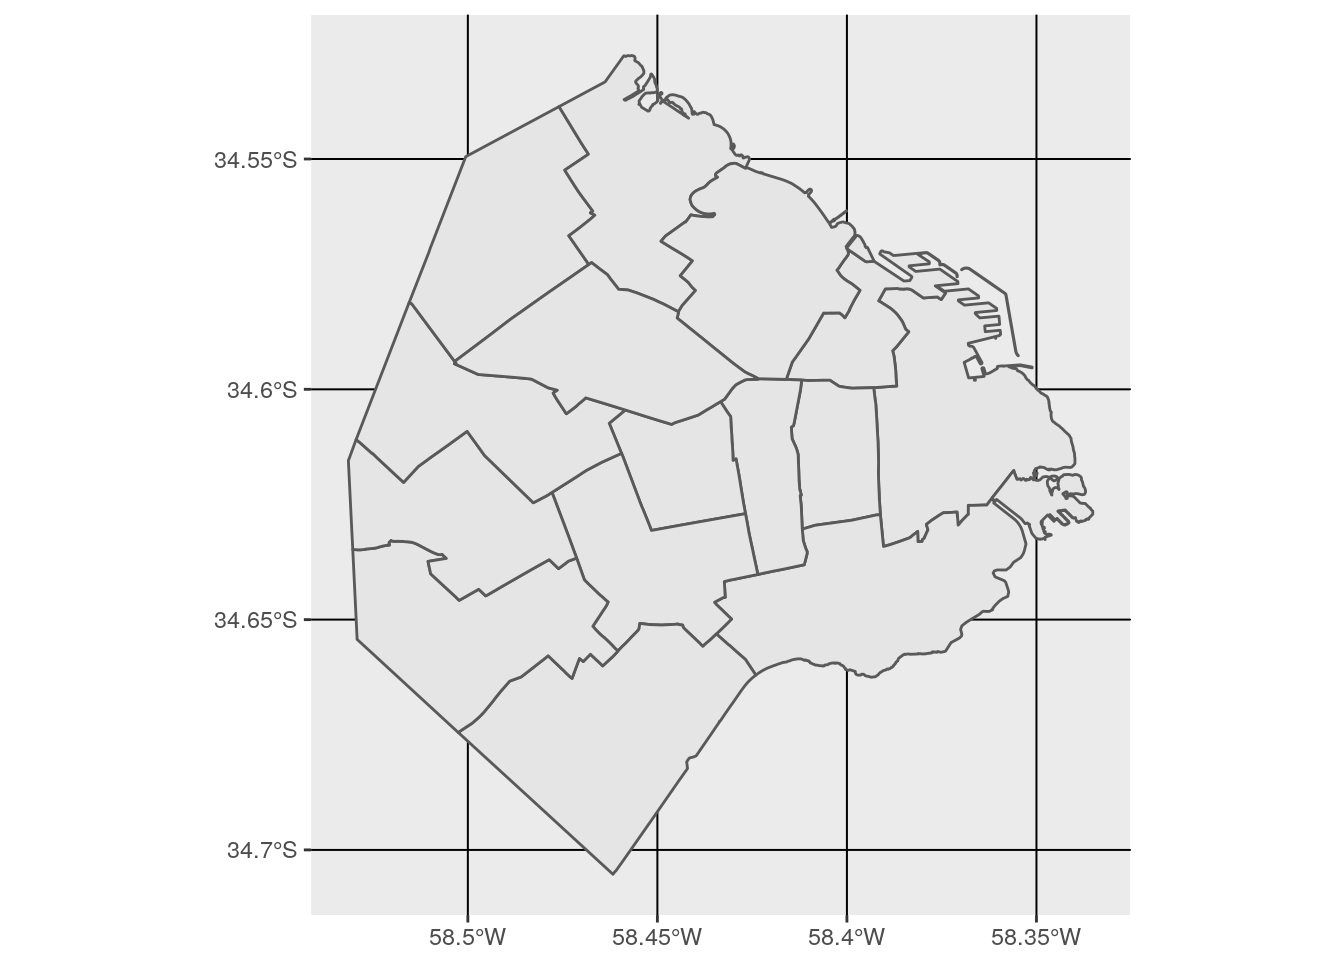
\includegraphics{ciencia_de_datos_para_gente_sociable_files/figure-latex/unnamed-chunk-83-1.pdf}

Lo que hicimos fue pedirle a ggplot que dibuje un punto por cada fila
(representando a cada comuna), con la posición en el eje de las
\texttt{x} según su población, y en el eje de las \texttt{y} según la
cantidad de contactos registrados. Estas referencias estéticas
(\emph{aesthetics} en inglés) son las que van dentro de la función
\texttt{aes()} en
\texttt{geom\_point(aes(x\ =\ POBLACION,\ y\ =\ miles\_contactos))}

Primer sorpresa: ¡en el extremo superior derecho hay una comuna que se
sale de la norma! Su relación población/reclamos es muy diferente a la
de todas las demás. Podemos identificarla, pidiendo a ggplot que agregue
una variable más a la visualización -la comuna. Siendo un gráfico en dos
dimensiones, ya no podemos usar la posición para representar un valor;
tanto la posición horizontal como la vertical están siendo usadas por
población y total. Nuestras opciones son codificar la comuna por color,
forma o tamaño del punto. A pesar de que son identificadas con números,
las comunas son una variable categórica: no tiene sentido decir que la
comuna 1 es ``menor'' que la comuna 7. Par las variables categóricas, el
color suele ser una buena opción de codificación.

Lo hacemos agregando un parámetro \texttt{color} dentro de
\texttt{aes()}. Tal como hicimos en el capítulo 2, usamos
\texttt{factor(COMUNA)} en lugar de \texttt{COMUNA} a secas para
indicarle a R que queremos que trate a la variable como categórica:

\begin{Shaded}
\begin{Highlighting}[]
\KeywordTok{ggplot}\NormalTok{(contactos_por_comuna) }\OperatorTok{+}\StringTok{ }
\StringTok{    }\KeywordTok{geom_point}\NormalTok{(}\KeywordTok{aes}\NormalTok{(}\DataTypeTok{x =}\NormalTok{ POBLACION, }\DataTypeTok{y =}\NormalTok{ miles_contactos, }\DataTypeTok{color =} \KeywordTok{factor}\NormalTok{(COMUNA)))}
\end{Highlighting}
\end{Shaded}

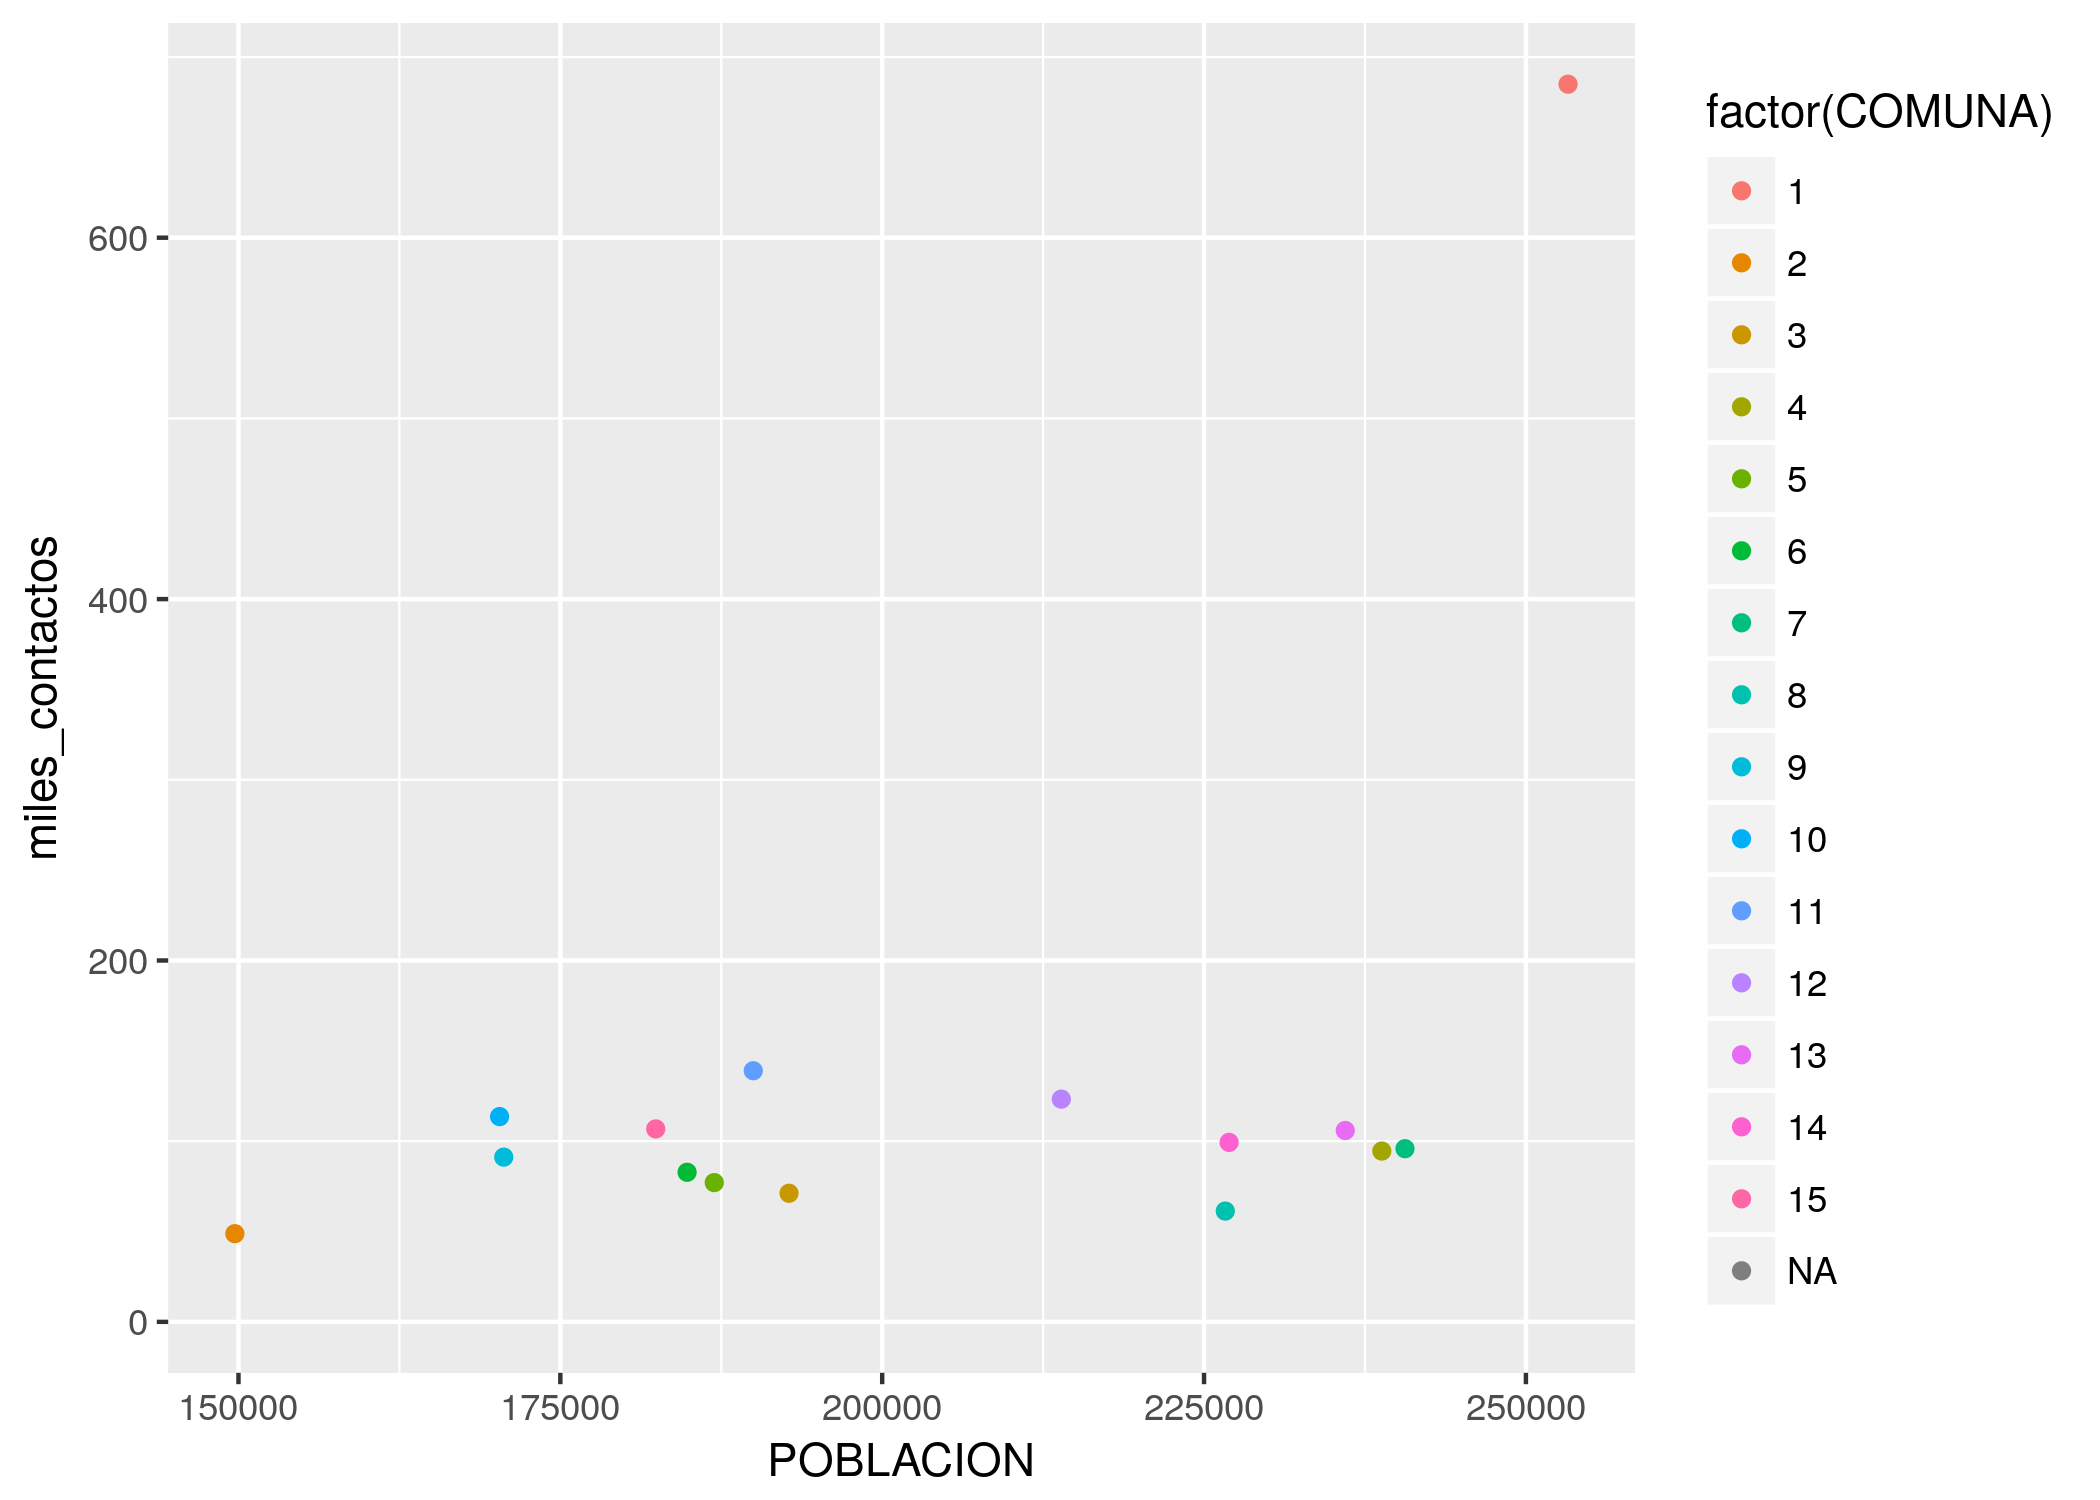
\includegraphics{ciencia_de_datos_para_gente_sociable_files/figure-latex/unnamed-chunk-84-1.pdf}

En ese caso, no es tan fácil discernir cuál es cuál, pero mirando con
cuidado descubrimos que la comuna 1 es el \emph{outlier}, el valor fuera
de lo común. Lo que nos pasa aquí es que tenemos demasiadas categorías,
con lo cual cada una tiene su propio color pero el rango cromático no
alcanza para darle a cada una un tono bien distinto al de las demás.

Si necesitamos generar un gráfico que no deje lugar a dudas, lo
resolvemos usando un método alternativo para el scatterplot. En lugar de
dibujar puntos, podemos poner etiquetas con el nombre de cada comuna.

En lugar de

\begin{Shaded}
\begin{Highlighting}[]
\KeywordTok{ggplot}\NormalTok{(contactos_por_comuna) }\OperatorTok{+}\StringTok{ }
\StringTok{    }\KeywordTok{geom_point}\NormalTok{(}\KeywordTok{aes}\NormalTok{(}\DataTypeTok{x =}\NormalTok{ POBLACION, }\DataTypeTok{y =}\NormalTok{ miles_contactos, }\DataTypeTok{color =} \KeywordTok{factor}\NormalTok{(COMUNA)))}
\end{Highlighting}
\end{Shaded}

usamos

\begin{Shaded}
\begin{Highlighting}[]
\KeywordTok{ggplot}\NormalTok{(contactos_por_comuna) }\OperatorTok{+}
\StringTok{    }\KeywordTok{geom_label}\NormalTok{(}\KeywordTok{aes}\NormalTok{(}\DataTypeTok{x =}\NormalTok{ POBLACION, }\DataTypeTok{y =}\NormalTok{ miles_contactos, }\DataTypeTok{label =} \KeywordTok{factor}\NormalTok{(COMUNA)))}
\end{Highlighting}
\end{Shaded}

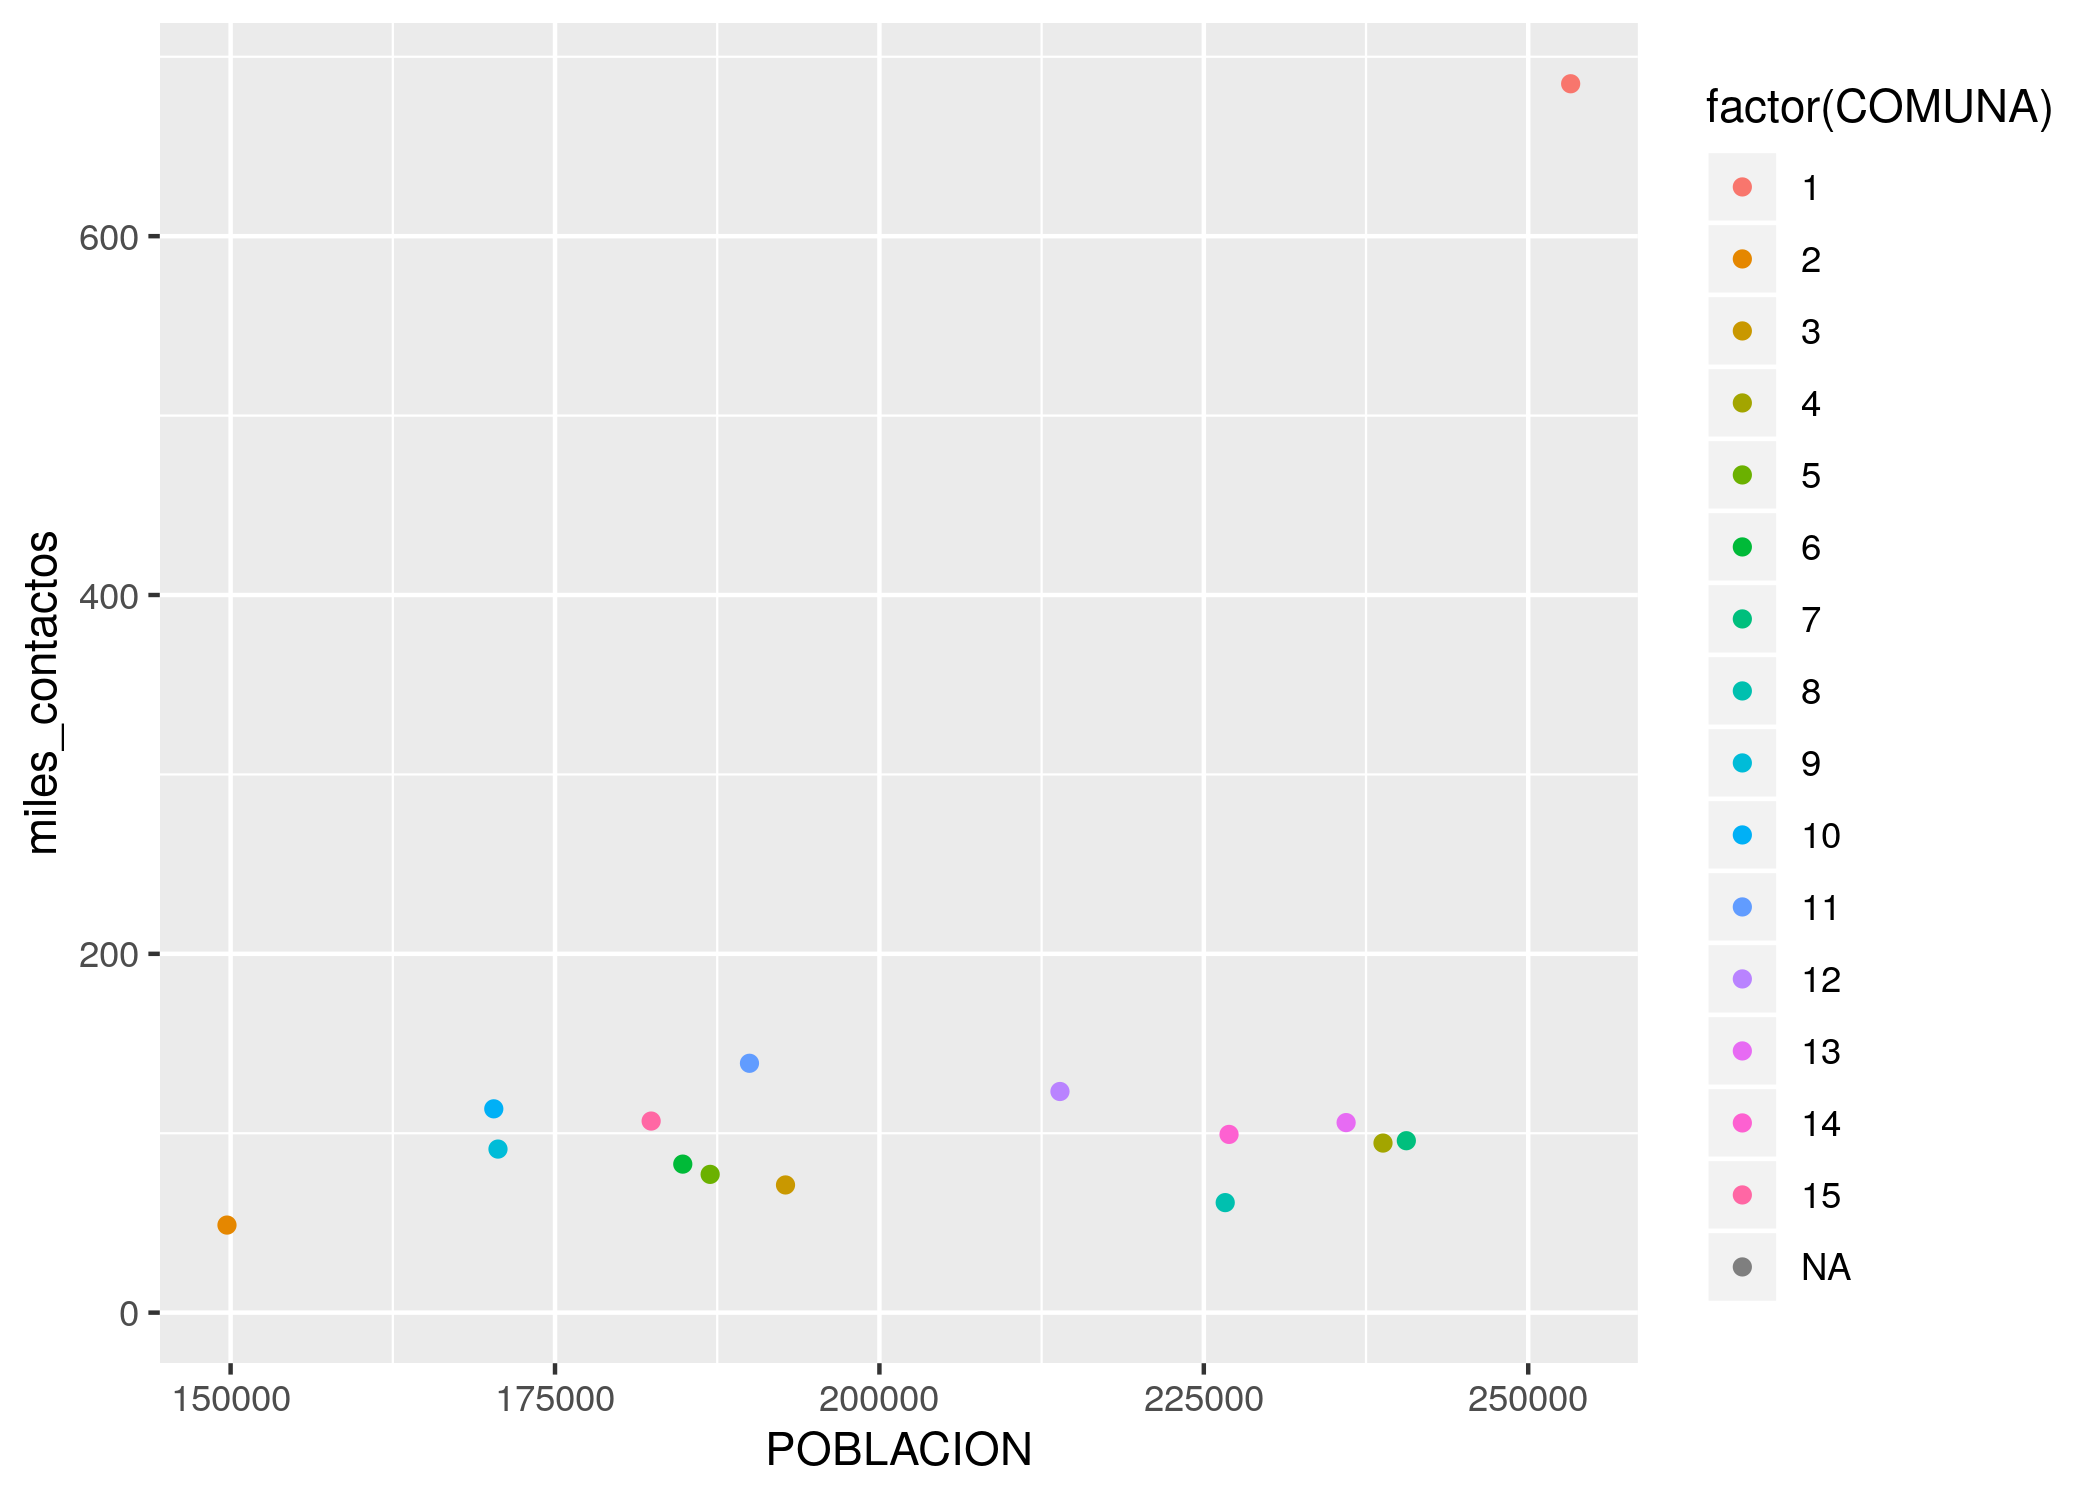
\includegraphics{ciencia_de_datos_para_gente_sociable_files/figure-latex/unnamed-chunk-86-1.pdf}

Volvamos a nuestros puntos para practicar dos codificaciones estéticas
que no hemos probado, color y tamaño.

Para dejar aún más clara la diferencia de reclamos entre comunas,
podríamos usar el tamaño (\emph{size}) de cada punto para representar
esa variable, además de su altura en el gráfico.

\begin{Shaded}
\begin{Highlighting}[]
\KeywordTok{ggplot}\NormalTok{(contactos_por_comuna) }\OperatorTok{+}\StringTok{ }
\StringTok{    }\KeywordTok{geom_point}\NormalTok{(}\KeywordTok{aes}\NormalTok{(}\DataTypeTok{x =}\NormalTok{ POBLACION, }\DataTypeTok{y =}\NormalTok{ miles_contactos, }\DataTypeTok{size =}\NormalTok{ miles_contactos))}
\end{Highlighting}
\end{Shaded}

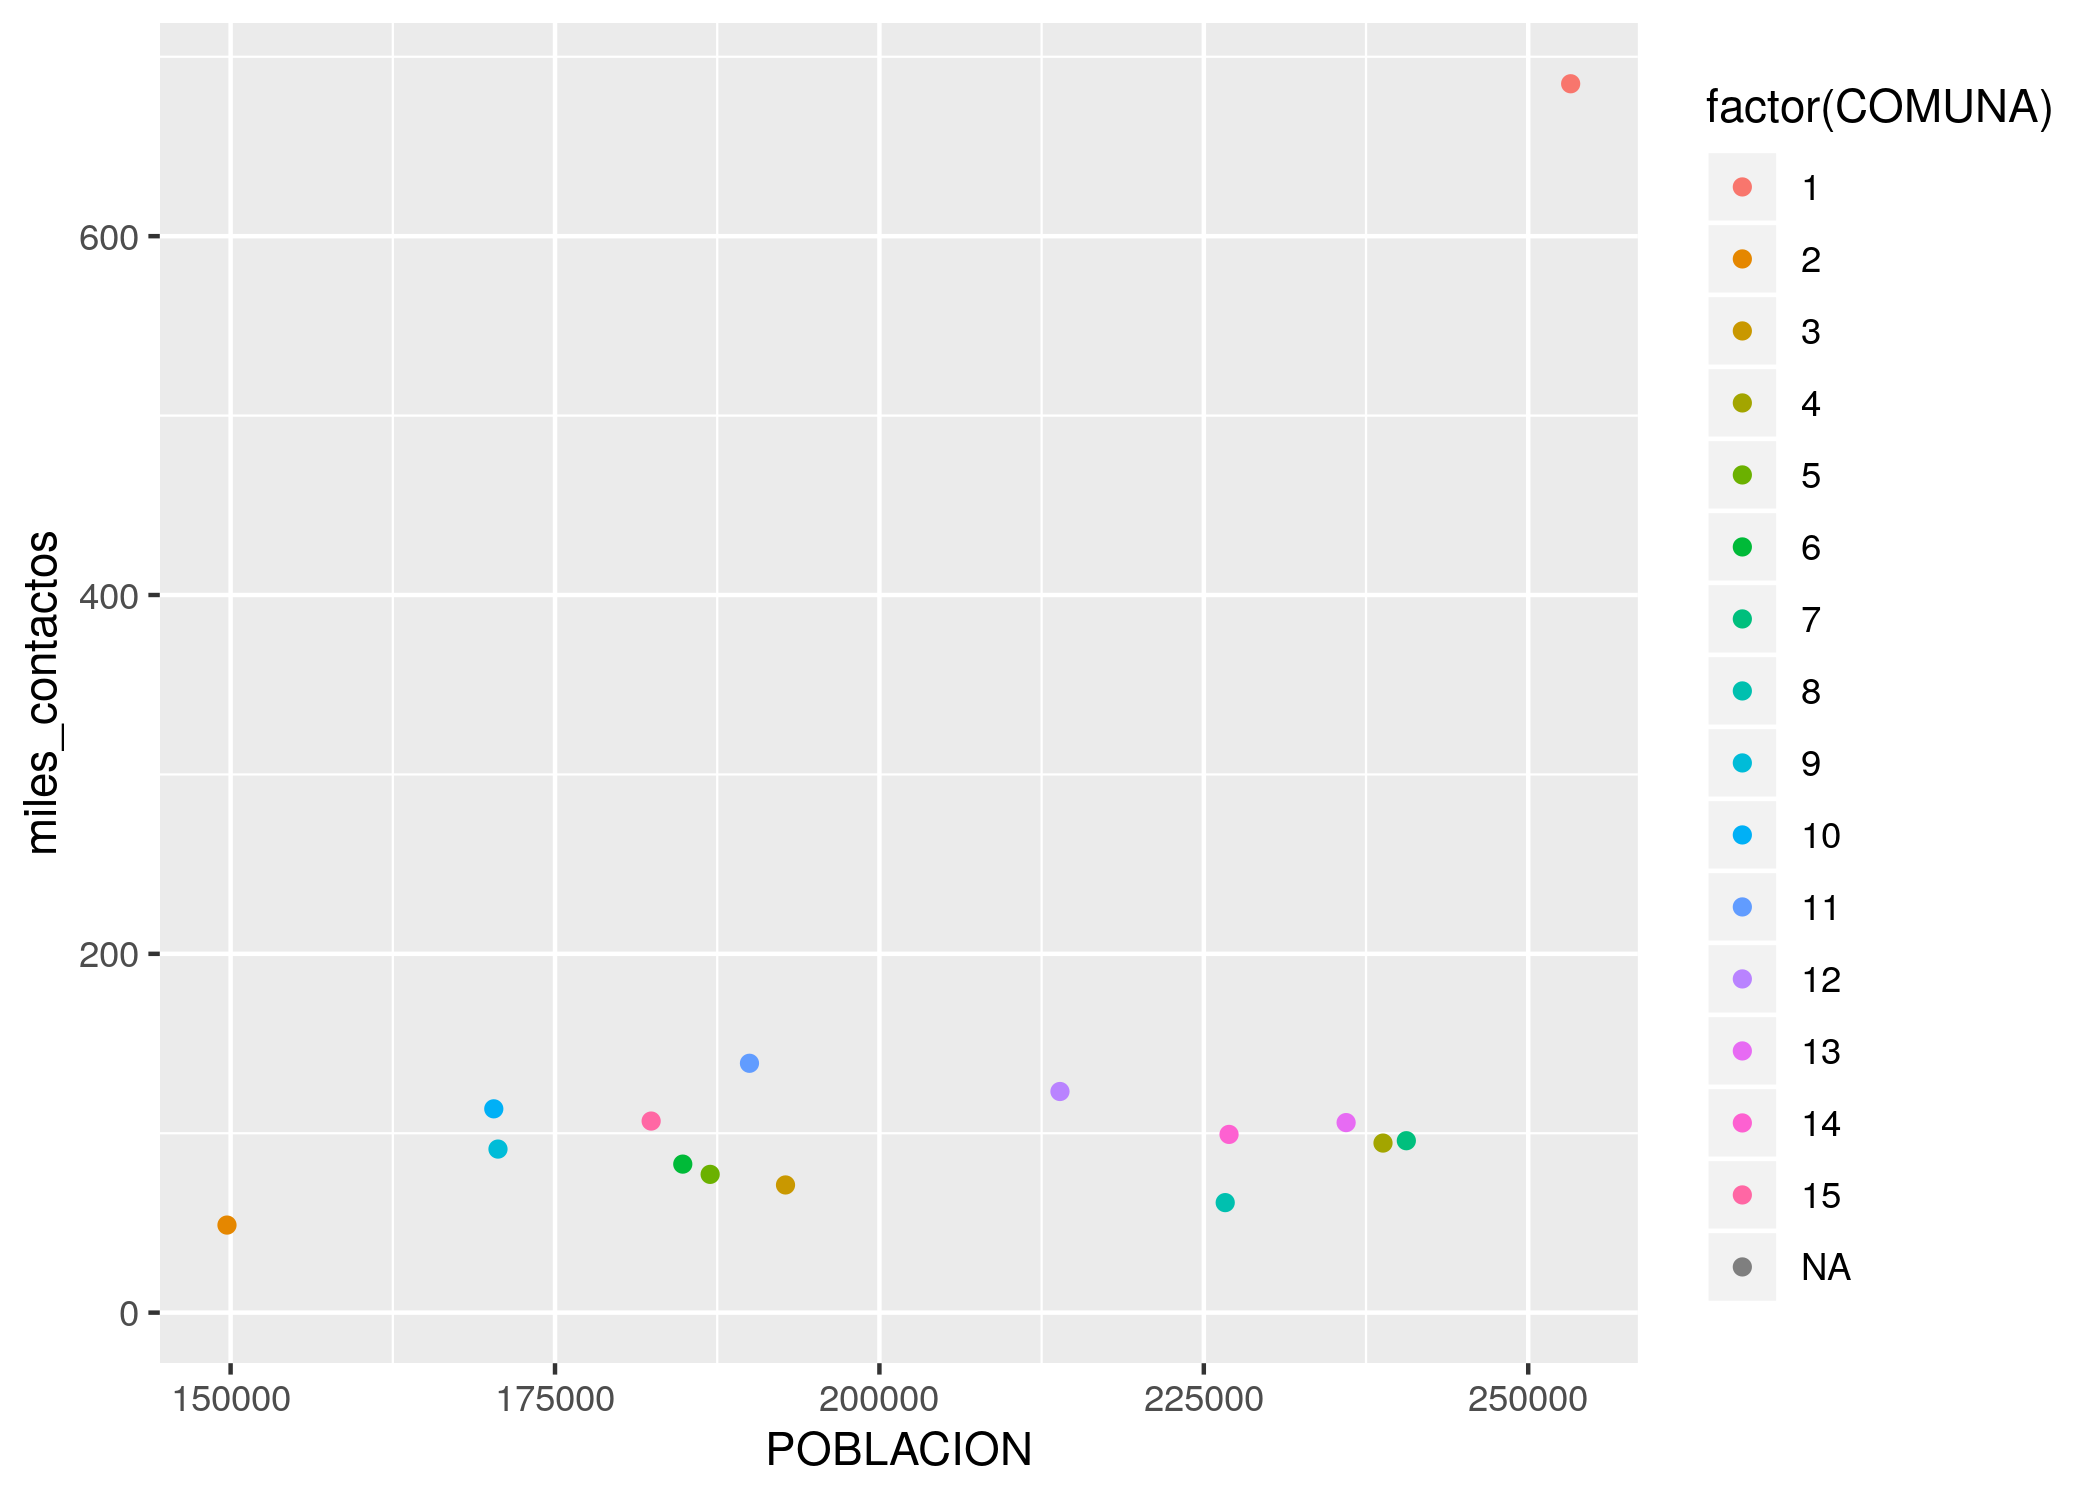
\includegraphics{ciencia_de_datos_para_gente_sociable_files/figure-latex/unnamed-chunk-87-1.pdf}

Y para distinguir cuál es cuál, podemos pedirle a ggplot que cambie la
forma (\emph{shape}) de cada punto según la comuna a la que corresponde.

\begin{Shaded}
\begin{Highlighting}[]
\KeywordTok{ggplot}\NormalTok{(contactos_por_comuna) }\OperatorTok{+}\StringTok{ }
\StringTok{    }\KeywordTok{geom_point}\NormalTok{(}\KeywordTok{aes}\NormalTok{(}\DataTypeTok{x =}\NormalTok{ POBLACION, }\DataTypeTok{y =}\NormalTok{ miles_contactos, }\DataTypeTok{shape =} \KeywordTok{factor}\NormalTok{(COMUNA)))}
\end{Highlighting}
\end{Shaded}

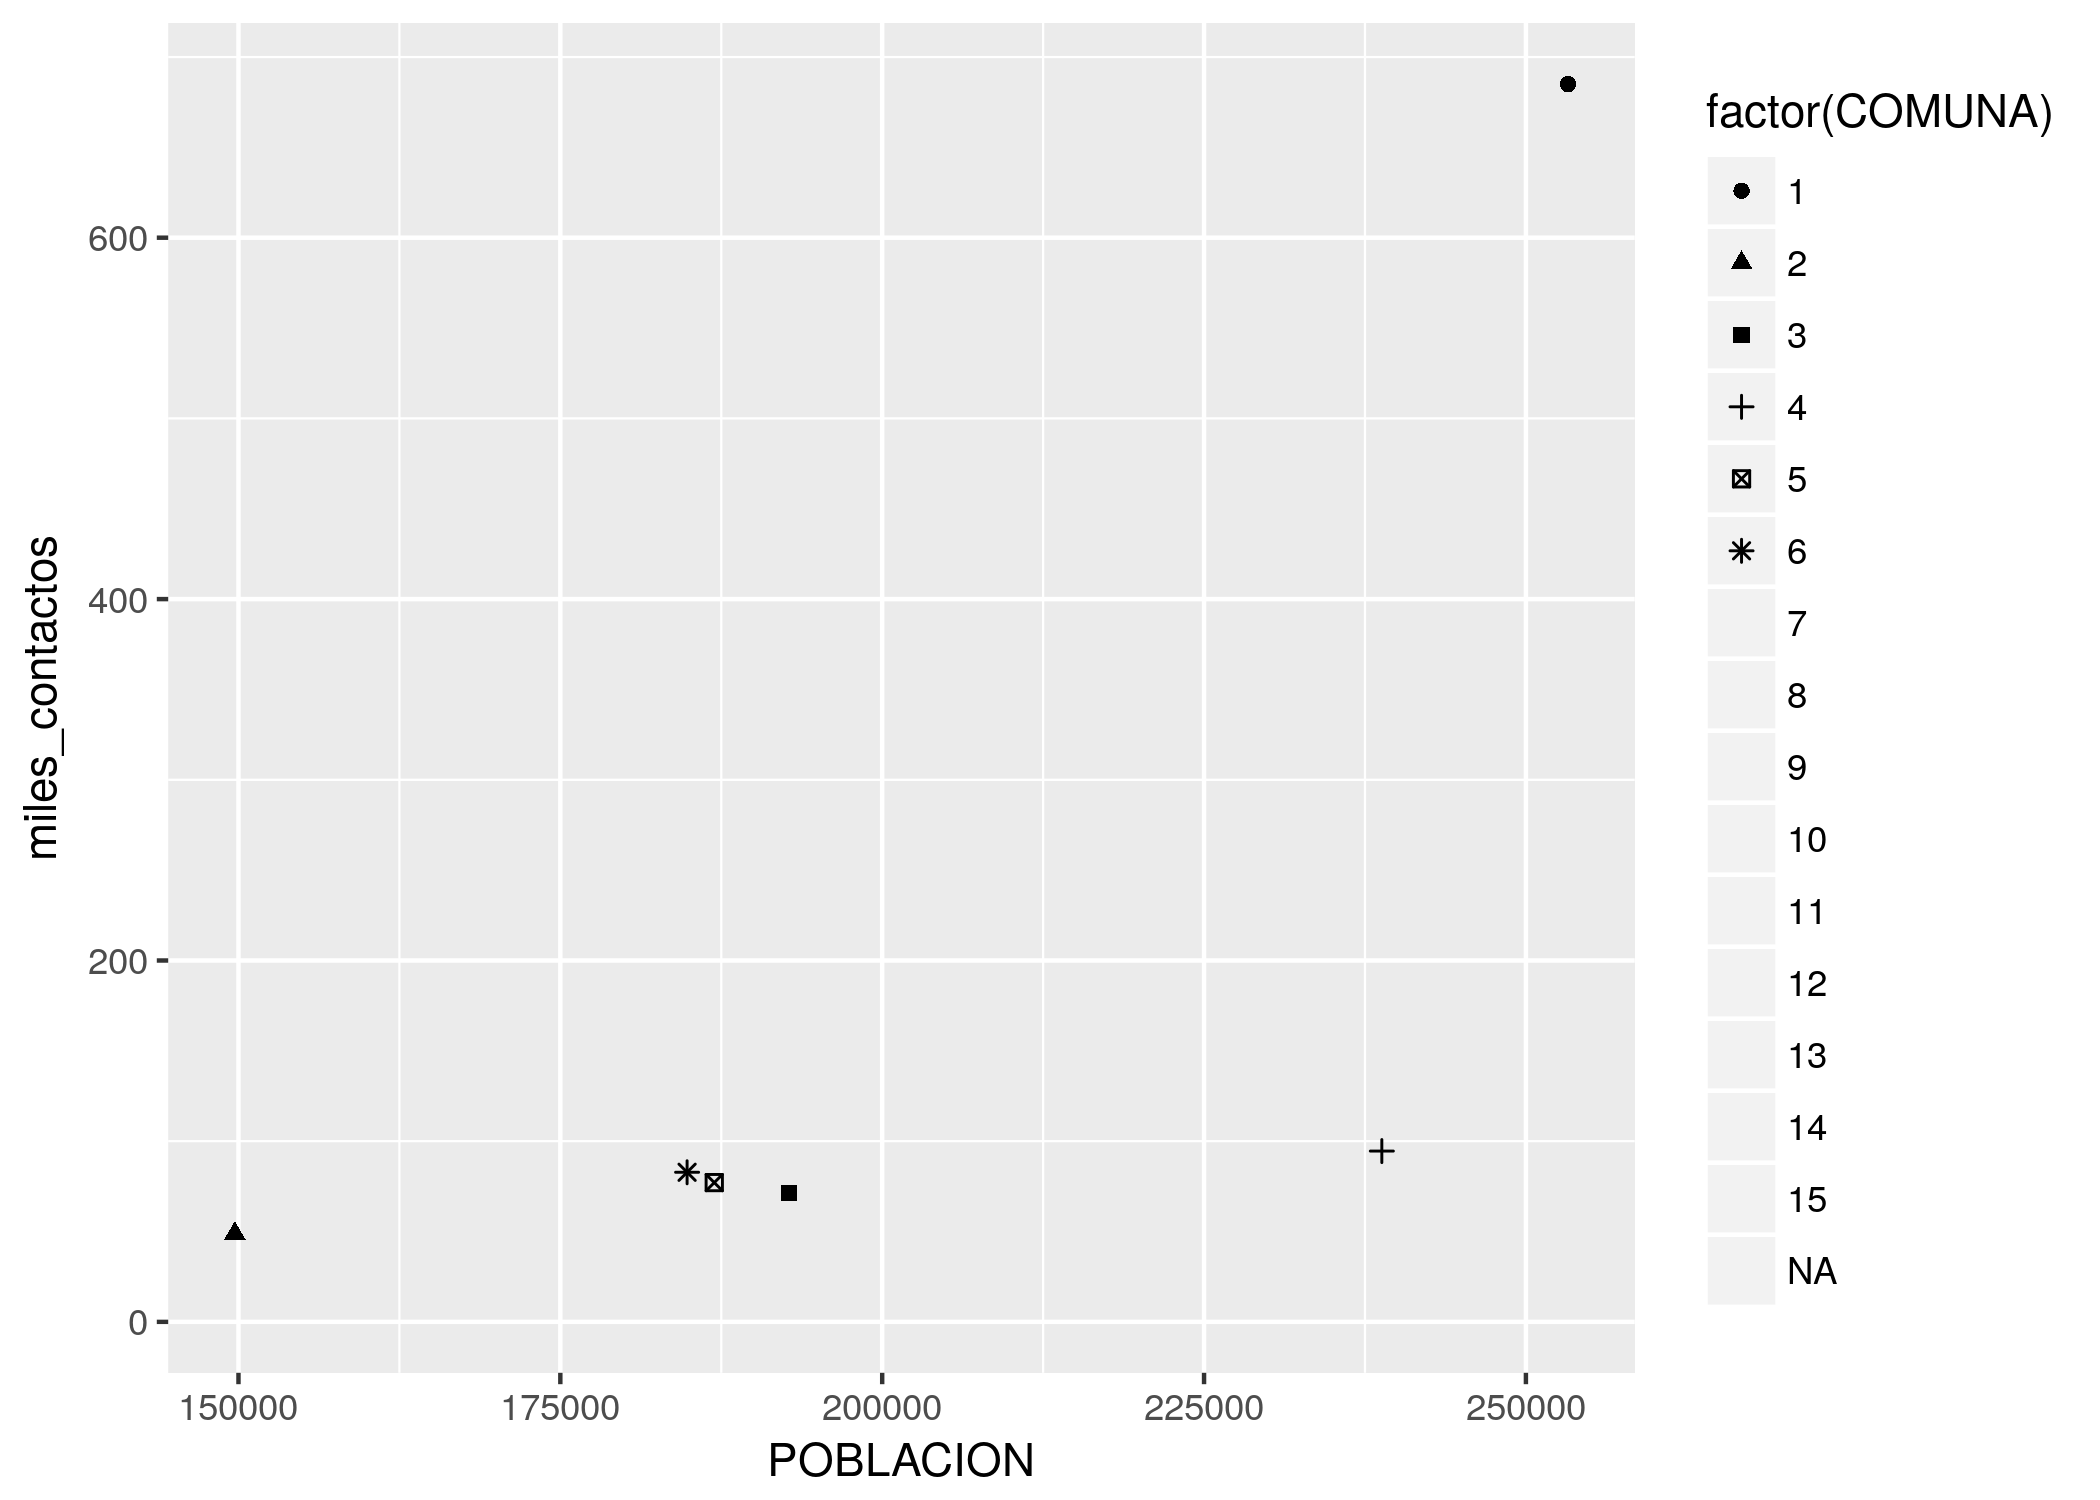
\includegraphics{ciencia_de_datos_para_gente_sociable_files/figure-latex/unnamed-chunk-88-1.pdf}

¡Hey, sólo aparecen seis de las comunas! \texttt{ggplot()} usa cómo
máximo 6 formas distintas, debido a que una cantidad mayor sería de
veras muy difícil de discernir para nuestros pobres ojos. Moraleja: la
estética \texttt{shape} sirve sólo cuando manejamos pocas categorías. De
todas formas -en mi opinión- es el método de codificación que menos
gracia tiene, así que no es grave que su utilidad sea limitada.

\section{Ajustando color y tamaño}\label{ajustando-color-y-tamano}

Hemos visto que especificando atributos estéticos y las variables que
representan dentro de \texttt{aes()} podemos ajustas posición, tamaño,
color y hasta la forma de los puntos de acuerdo a sus valores. Pero,
¿qué pasa si queremos usar un tamaño o un color arbitrario para nuestros
puntos? Es decir, si no nos gusta el color negro y queremos que sean
todos azules, o si nos parece que se ven pequeños y queremos que sean
todos un poco más grandes. Fácil: definimos el \texttt{color} o
\texttt{size} que queremos por fuera de las función \texttt{aes()}, y
será aplicado a todos los puntos.

\begin{Shaded}
\begin{Highlighting}[]
\KeywordTok{ggplot}\NormalTok{(contactos_por_comuna) }\OperatorTok{+}\StringTok{ }
\StringTok{    }\KeywordTok{geom_point}\NormalTok{(}\KeywordTok{aes}\NormalTok{(}\DataTypeTok{x =}\NormalTok{ POBLACION, }\DataTypeTok{y =}\NormalTok{ miles_contactos), }\DataTypeTok{color =} \StringTok{"blue"}\NormalTok{)}
\end{Highlighting}
\end{Shaded}

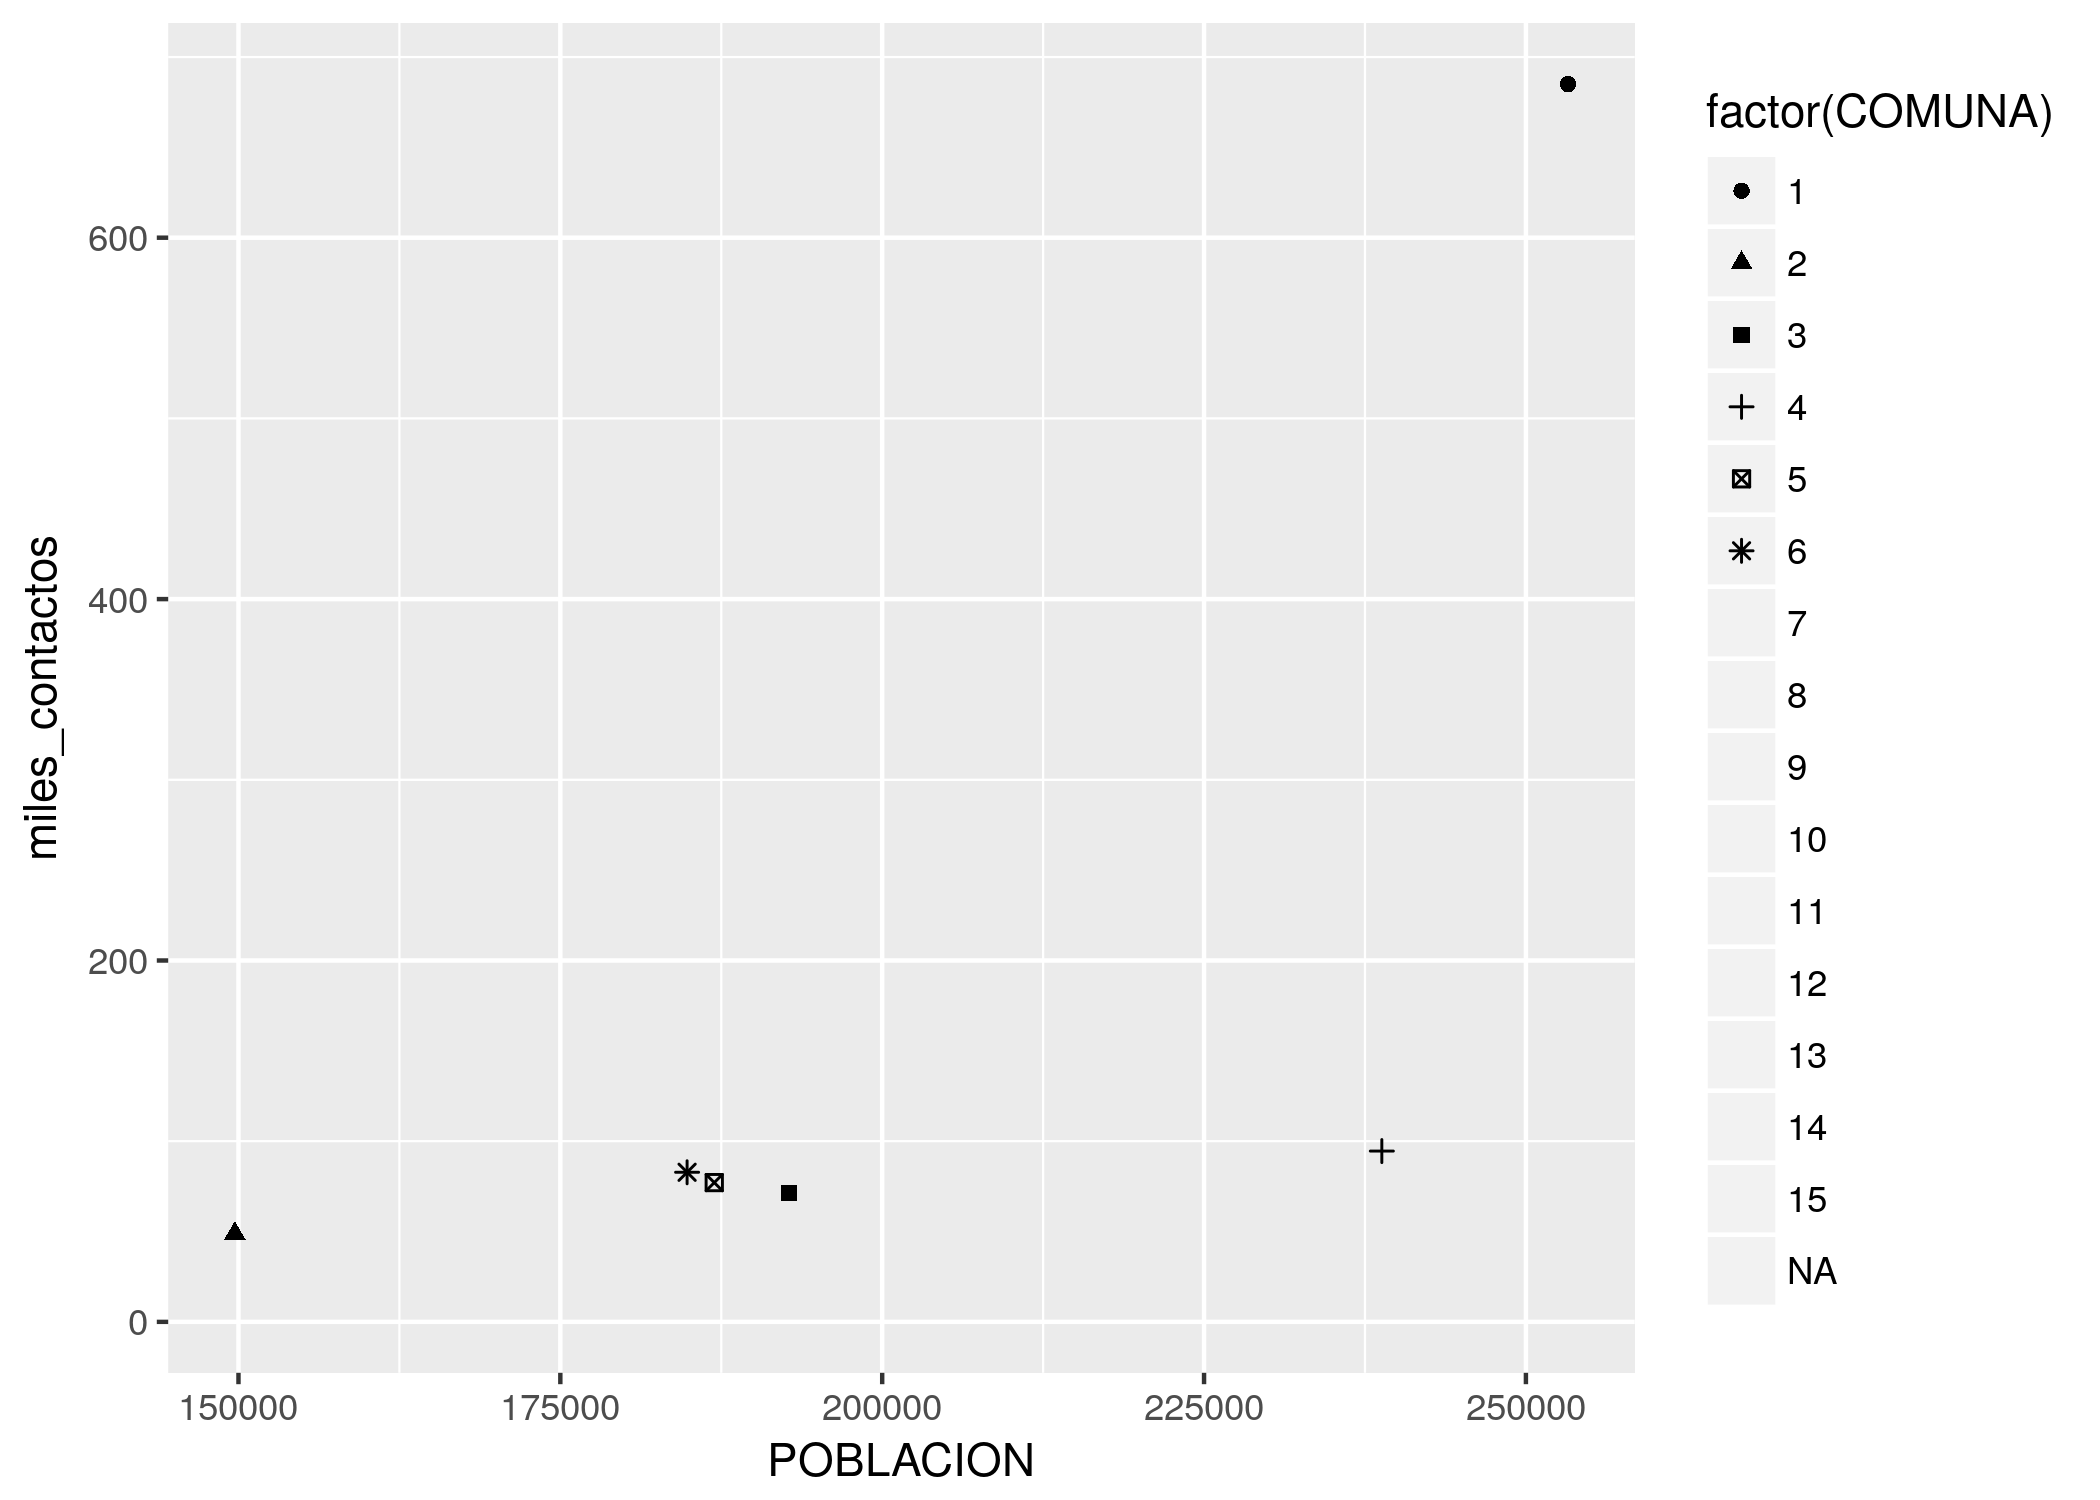
\includegraphics{ciencia_de_datos_para_gente_sociable_files/figure-latex/unnamed-chunk-89-1.pdf}

Obsérvese que \texttt{color\ =\ "blue"} está escrito por fuera de los
paréntesis de \texttt{aes()}. De paso, hicimos uso de una característica
muy práctica de R: reconoce un montón de colores por su nombre, siempre
que los escribamos entre comillas. Si le decimos
\texttt{color\ =\ "blue"}, \texttt{color\ =\ "red"},
\texttt{color\ =\ "yellow"}, etc., sabe de que hablamos. Una lista de
todos los colores que R reconoce, ideal como referencia, se puede
encontrar en \url{http://www.stat.columbia.edu/~tzheng/files/Rcolor.pdf}
; ¡son más de 600!.

Tras un vistazo a la lista, me decido por ``darkolivegreen4'':

\begin{Shaded}
\begin{Highlighting}[]
\KeywordTok{ggplot}\NormalTok{(contactos_por_comuna) }\OperatorTok{+}\StringTok{ }
\StringTok{    }\KeywordTok{geom_point}\NormalTok{(}\KeywordTok{aes}\NormalTok{(}\DataTypeTok{x =}\NormalTok{ POBLACION, }\DataTypeTok{y =}\NormalTok{ miles_contactos), }\DataTypeTok{color =} \StringTok{"darkolivegreen4"}\NormalTok{)}
\end{Highlighting}
\end{Shaded}

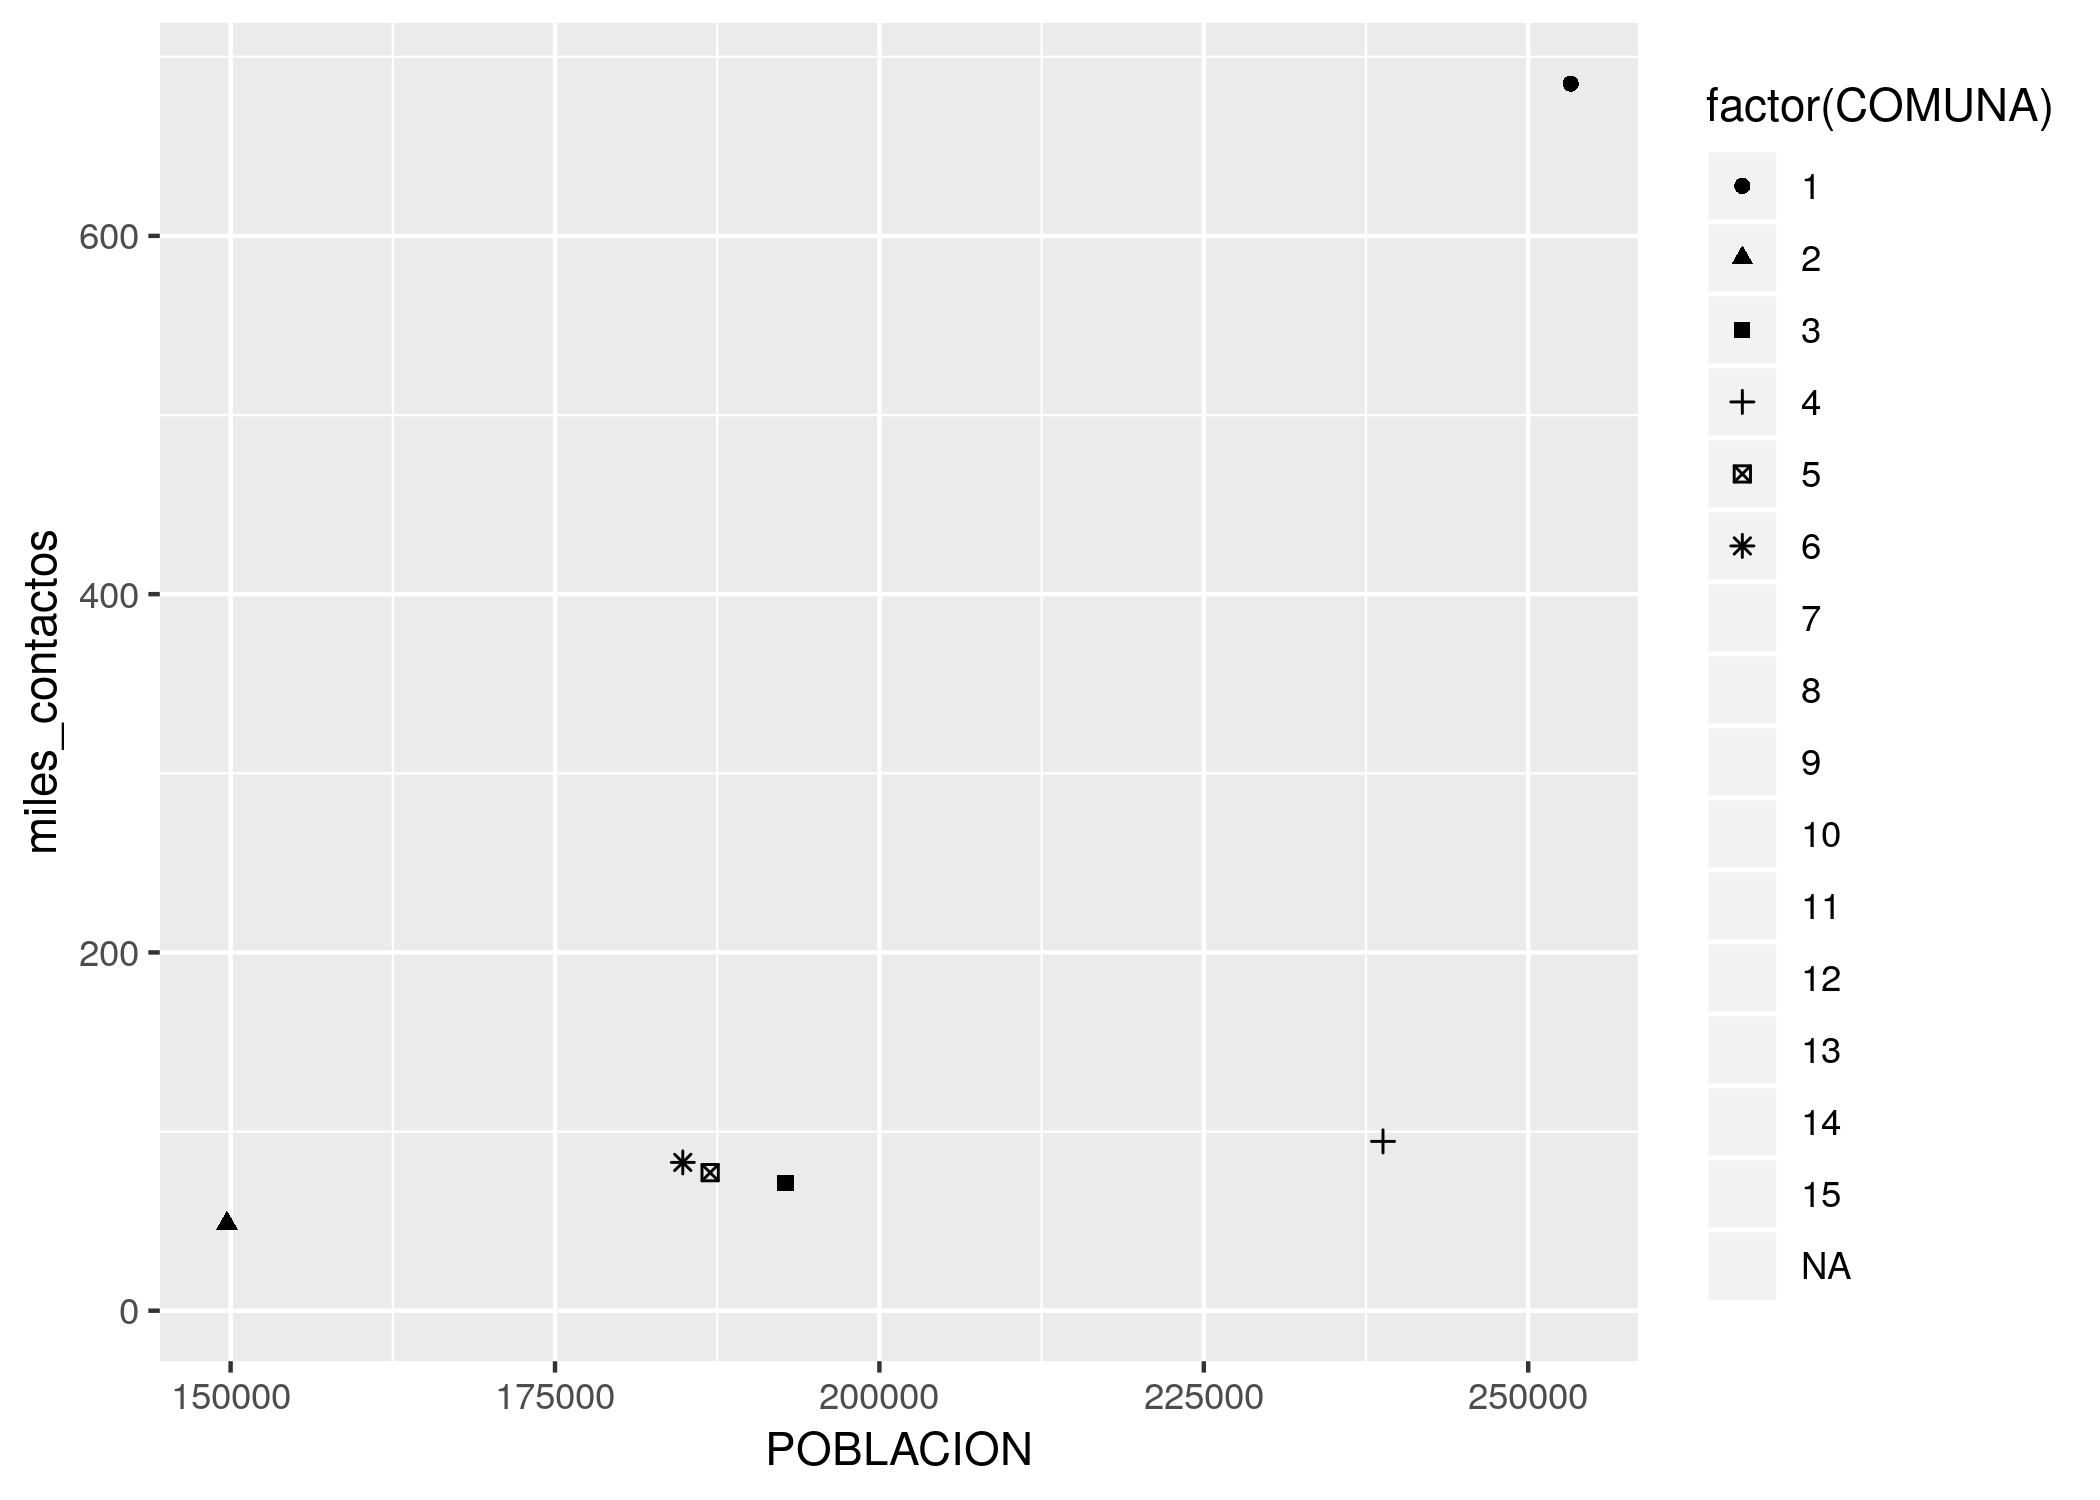
\includegraphics{ciencia_de_datos_para_gente_sociable_files/figure-latex/unnamed-chunk-90-1.pdf}

Bellísimo.

En cuanto al tamaño, la fórmula es la misma:

\begin{Shaded}
\begin{Highlighting}[]
\KeywordTok{ggplot}\NormalTok{(contactos_por_comuna) }\OperatorTok{+}\StringTok{ }
\StringTok{    }\KeywordTok{geom_point}\NormalTok{(}\KeywordTok{aes}\NormalTok{(}\DataTypeTok{x =}\NormalTok{ POBLACION, }\DataTypeTok{y =}\NormalTok{ miles_contactos), }\DataTypeTok{size =} \DecValTok{5}\NormalTok{)}
\end{Highlighting}
\end{Shaded}

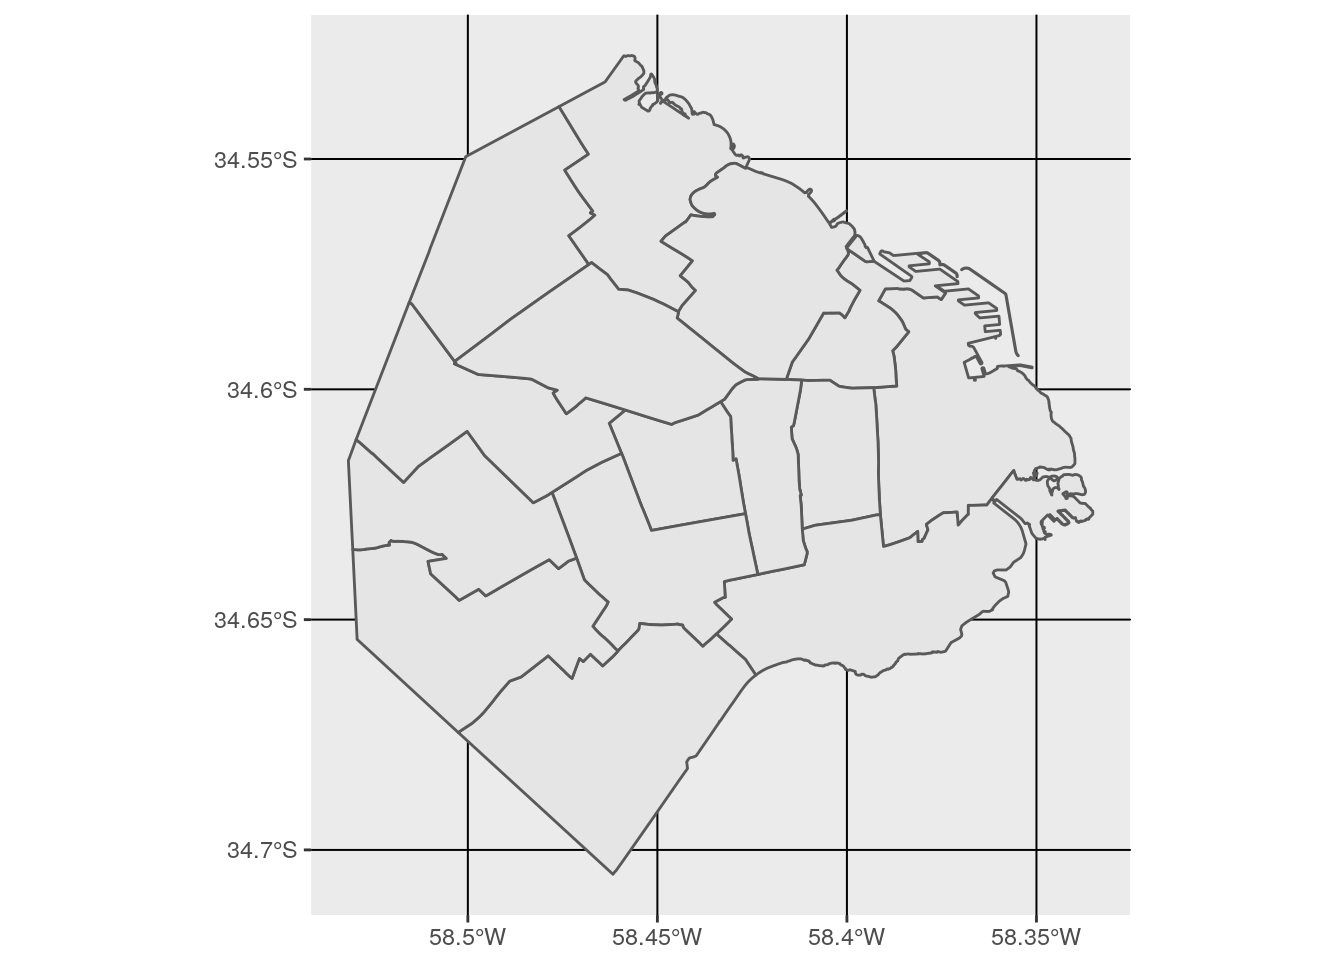
\includegraphics{ciencia_de_datos_para_gente_sociable_files/figure-latex/unnamed-chunk-91-1.pdf}

El valor de \texttt{size} se da en píxeles. Es una medida difícil de
estimar antes de ver el resultado, pero es cuestión de probar algunos
valores distintos hasta encontrar el que nos va bien. Por supuesto,
podemos ajustar varios, o todos, los atributos a la vez

\begin{Shaded}
\begin{Highlighting}[]
\KeywordTok{ggplot}\NormalTok{(contactos_por_comuna) }\OperatorTok{+}\StringTok{ }
\StringTok{    }\KeywordTok{geom_point}\NormalTok{(}\KeywordTok{aes}\NormalTok{(}\DataTypeTok{x =}\NormalTok{ POBLACION, }\DataTypeTok{y =}\NormalTok{ miles_contactos), }
               \DataTypeTok{size =} \DecValTok{9}\NormalTok{, }\DataTypeTok{color =} \StringTok{"chocolate3"}\NormalTok{, }\DataTypeTok{shape =} \DecValTok{0}\NormalTok{)}
\end{Highlighting}
\end{Shaded}

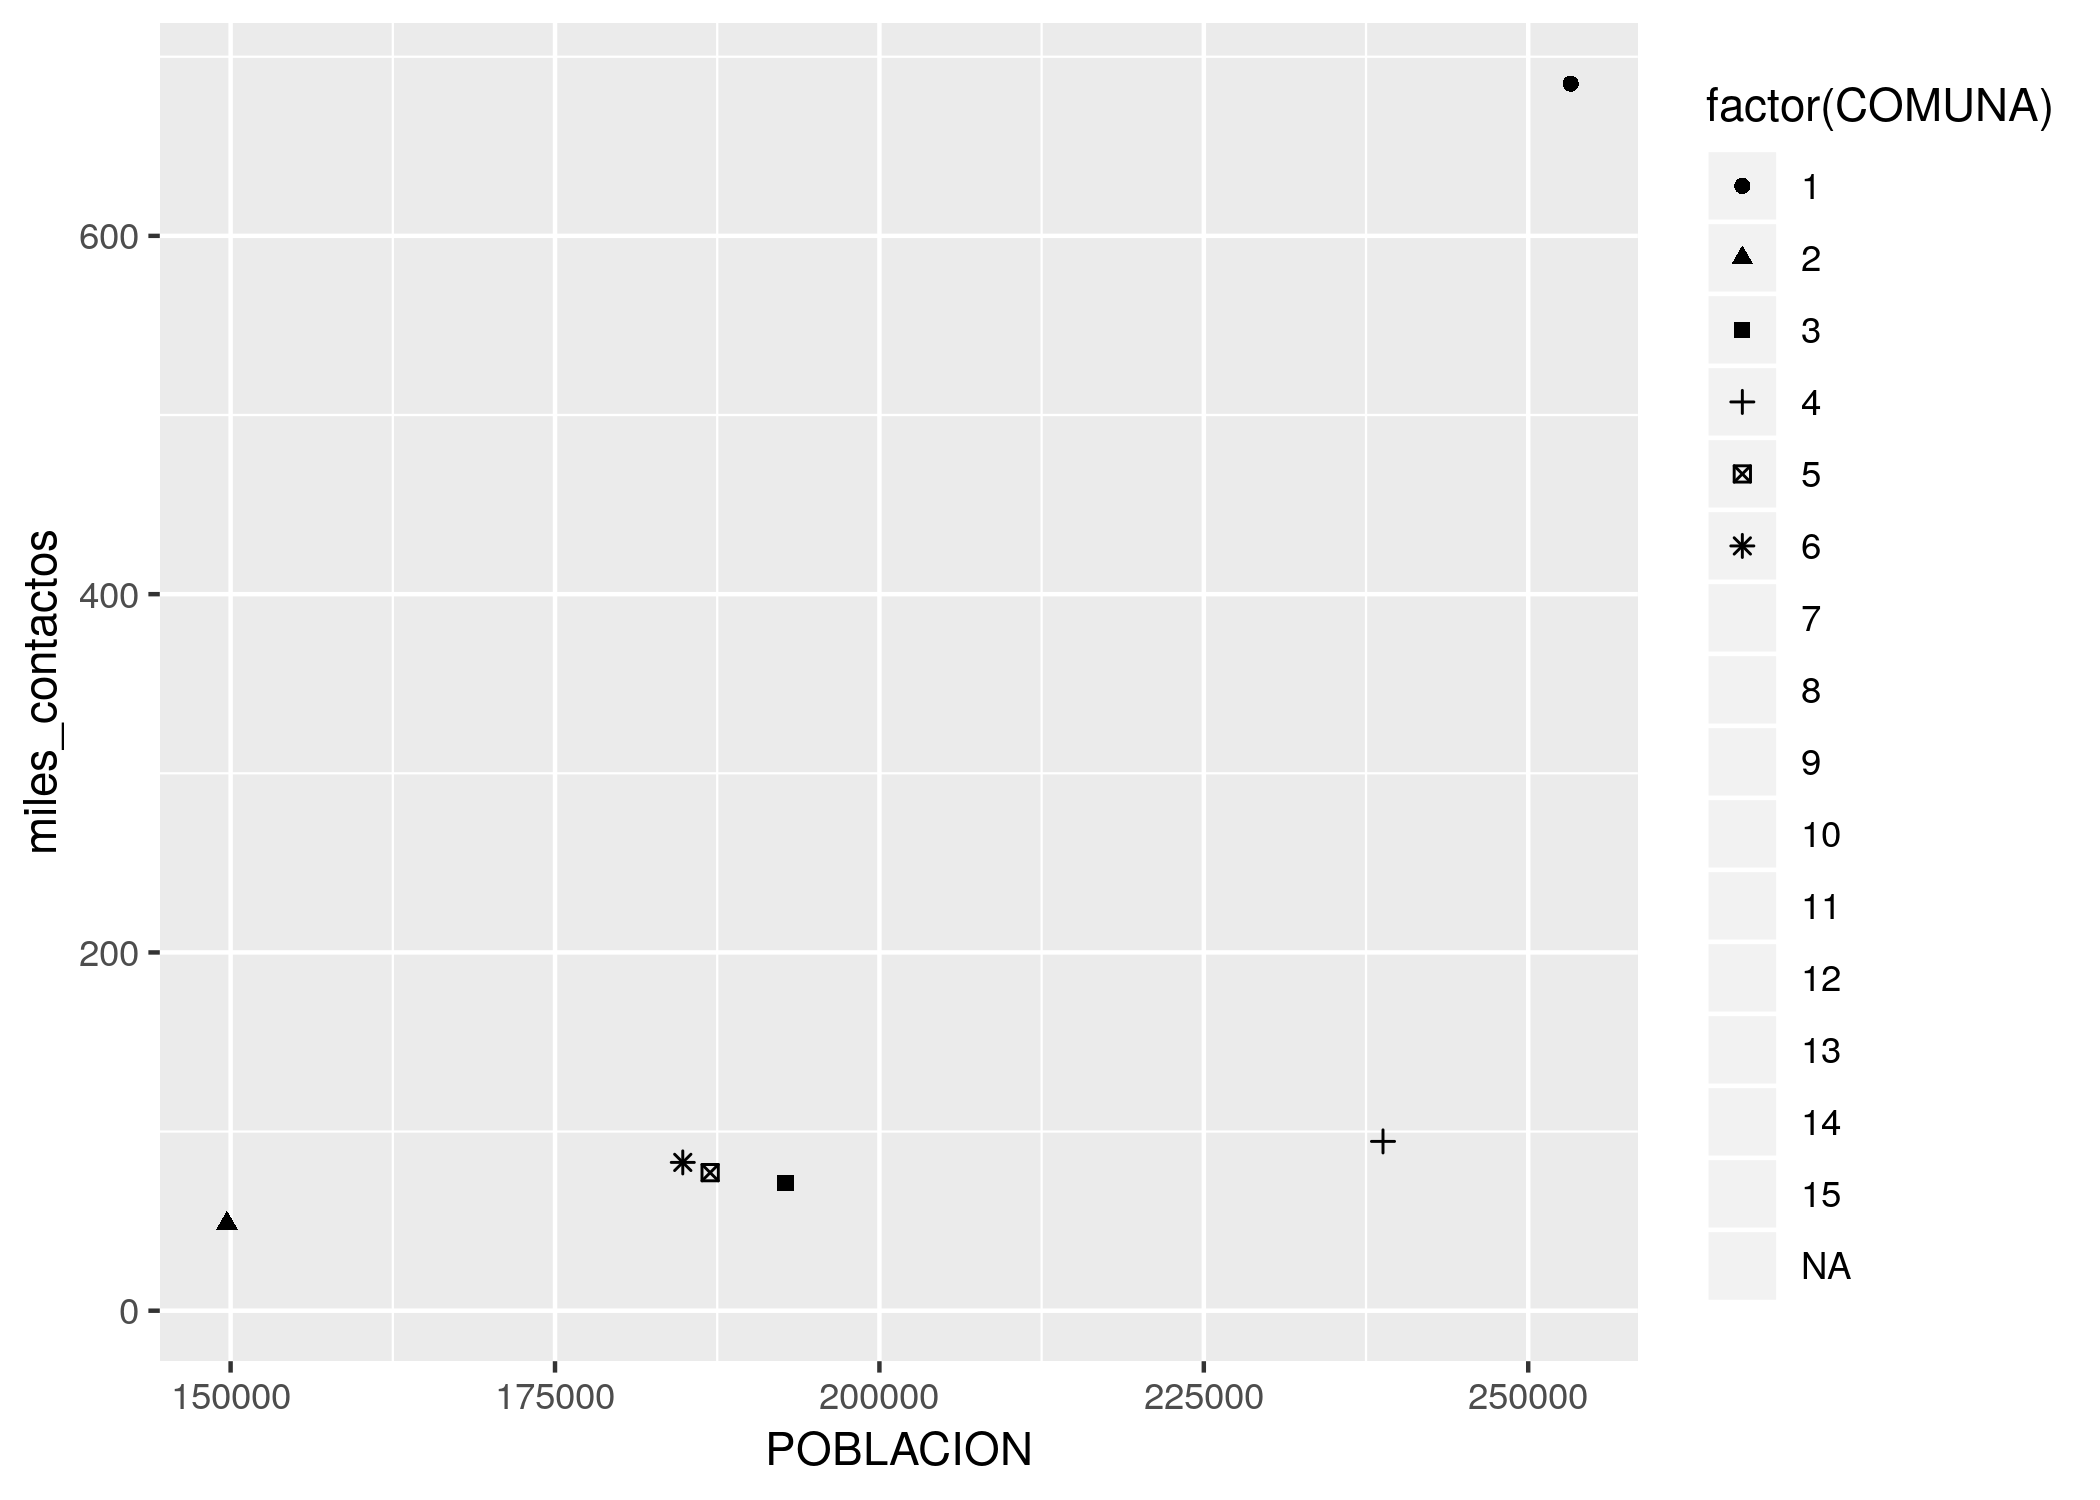
\includegraphics{ciencia_de_datos_para_gente_sociable_files/figure-latex/unnamed-chunk-92-1.pdf}

\section{Facetado}\label{facetado}

Ya sabemos como representar variables usando atributos estéticos. Con
esa técnica podemos mostrar con claridad dos o tres variables en un
plano bidimensional (nuestro gráfico). Pero cuando si queremos agregar
más atributos para codificar variables adicionales, la visualización
pierde legibilidad de inmediato. Por suerte existe otra técnica, que
podemos usar en combinación con la estética, para agregar aún más
variables: el facetado.

Las facetas son múltiples gráficos contiguos, con cada uno mostrando un
subconjunto de los datos. Son útiles sobre todo para variables
categóricas.

Practiquemos con un ejemplo. Sabemos que en la comuna 1 se registra una
cantidad de contactos de la ciudadanía mucho mayor que en las demás. ¿La
diferencia será igual para todas las categorías de contacto, o existe
alguna en particular que es la que inclina la balanza?

En nuestro dataframe original, el tipo de contacto aparece en la columna
``TIPO\_PRESTACION''. El nombre que eligieron no es del todo
informativo, pero \texttt{summary()} (recuerden siempre lo usamos para
explorar un dataset que no conocemos) nos da una pista:

\begin{Shaded}
\begin{Highlighting}[]
\KeywordTok{summary}\NormalTok{(atencion_ciudadano)}
\end{Highlighting}
\end{Shaded}

\begin{verbatim}
##     PERIODO                         RUBRO        TIPO_PRESTACION 
##  Min.   :201301   SANEAMIENTO URBANO   : 4589   DENUNCIA :21606  
##  1st Qu.:201309   TRANSPORTE Y TRANSITO: 4580   QUEJA    : 3914  
##  Median :201404   ARBOLADO             : 3122   RECLAMO  :21038  
##  Mean   :201401   ALUMBRADO            : 2918   SOLICITUD: 9662  
##  3rd Qu.:201503   PAVIMENTO            : 2411   TRAMITE  : 1211  
##  Max.   :201512   ESPACIO PUBLICO      : 1918                    
##                   (Other)              :37893                    
##          BARRIO          total              COMUNA      
##  PALERMO    : 2154   Min.   :    1.00   Min.   : 1.000  
##  BALVANERA  : 1961   1st Qu.:    1.00   1st Qu.: 4.000  
##  FLORES     : 1959   Median :    4.00   Median : 9.000  
##  CABALLITO  : 1872   Mean   :   34.85   Mean   : 8.119  
##  SAN NICOLAS: 1748   3rd Qu.:   16.00   3rd Qu.:12.000  
##  RECOLETA   : 1729   Max.   :19221.00   Max.   :15.000  
##  (Other)    :46008                      NA's   :63      
##      AÑO                MES           
##  Length:57431       Length:57431      
##  Class :character   Class :character  
##  Mode  :character   Mode  :character  
##                                       
##                                       
##                                       
## 
\end{verbatim}

``TIPO\_PRESTACION'' es la categoría más general, con sólo cinco niveles
- ``DENUNCIA'', ``QUEJA'', ``RECLAMO'', ``SOLICITUD'' y ``TRAMITE''. Las
otras variables categóricas, asumimos, representan subtipos.

Agrupamos entonces nuestra data por comuna y por tipo de contacto, sin
olvidar agregar luego los datos de población

\begin{Shaded}
\begin{Highlighting}[]
\NormalTok{contactos_por_comuna_y_tipo <-}\StringTok{ }\NormalTok{atencion_ciudadano }\OperatorTok\StringTok{ }
\StringTok{    }\KeywordTok{group_by}\NormalTok{(COMUNA, TIPO_PRESTACION) }\OperatorTok\StringTok{ }
\StringTok{    }\KeywordTok{summarise}\NormalTok{(}\DataTypeTok{miles_contactos =} \KeywordTok{sum}\NormalTok{(total) }\OperatorTok{/}\StringTok{ }\DecValTok{1000}\NormalTok{ ) }\OperatorTok\StringTok{ }
\StringTok{    }\KeywordTok{left_join}\NormalTok{(habitantes)}

\KeywordTok{head}\NormalTok{(contactos_por_comuna_y_tipo)}
\end{Highlighting}
\end{Shaded}

\begin{verbatim}
## # A tibble: 6 x 4
## # Groups:   COMUNA [2]
##   COMUNA TIPO_PRESTACION miles_contactos POBLACION
##    <int> <fct>                     <dbl>     <int>
## 1      1 DENUNCIA                   22.9    253271
## 2      1 QUEJA                      17.4    253271
## 3      1 RECLAMO                    55.7    253271
## 4      1 SOLICITUD                  20.9    253271
## 5      1 TRAMITE                   568      253271
## 6      2 DENUNCIA                   10.2    149720
\end{verbatim}

Listos para facetar. Producimos un scatterplot igual que antes, y le
agregamos una capa adicional con \texttt{facet\_wrap()}. La variable a
``facetar'', la que recibirá un gráfico por cada una de sus categorías,
siempre se escribe a continuación del signo \texttt{\textasciitilde{}};
en nuestro caso, queda como \texttt{\textasciitilde{}TIPO\_PRESTACION}.
El simbolillo en cuestión denota lo que en R se denomina una
\emph{fórmula} y ya nos lo cruzaremos de nuevo, pero par ahora no le
prestamos más atención.

\begin{Shaded}
\begin{Highlighting}[]
\KeywordTok{ggplot}\NormalTok{(contactos_por_comuna_y_tipo) }\OperatorTok{+}\StringTok{ }
\StringTok{    }\KeywordTok{geom_point}\NormalTok{(}\KeywordTok{aes}\NormalTok{(}\DataTypeTok{x =}\NormalTok{ POBLACION, }\DataTypeTok{y =}\NormalTok{ miles_contactos)) }\OperatorTok{+}
\StringTok{    }\KeywordTok{facet_wrap}\NormalTok{(}\OperatorTok{~}\NormalTok{TIPO_PRESTACION)}
\end{Highlighting}
\end{Shaded}

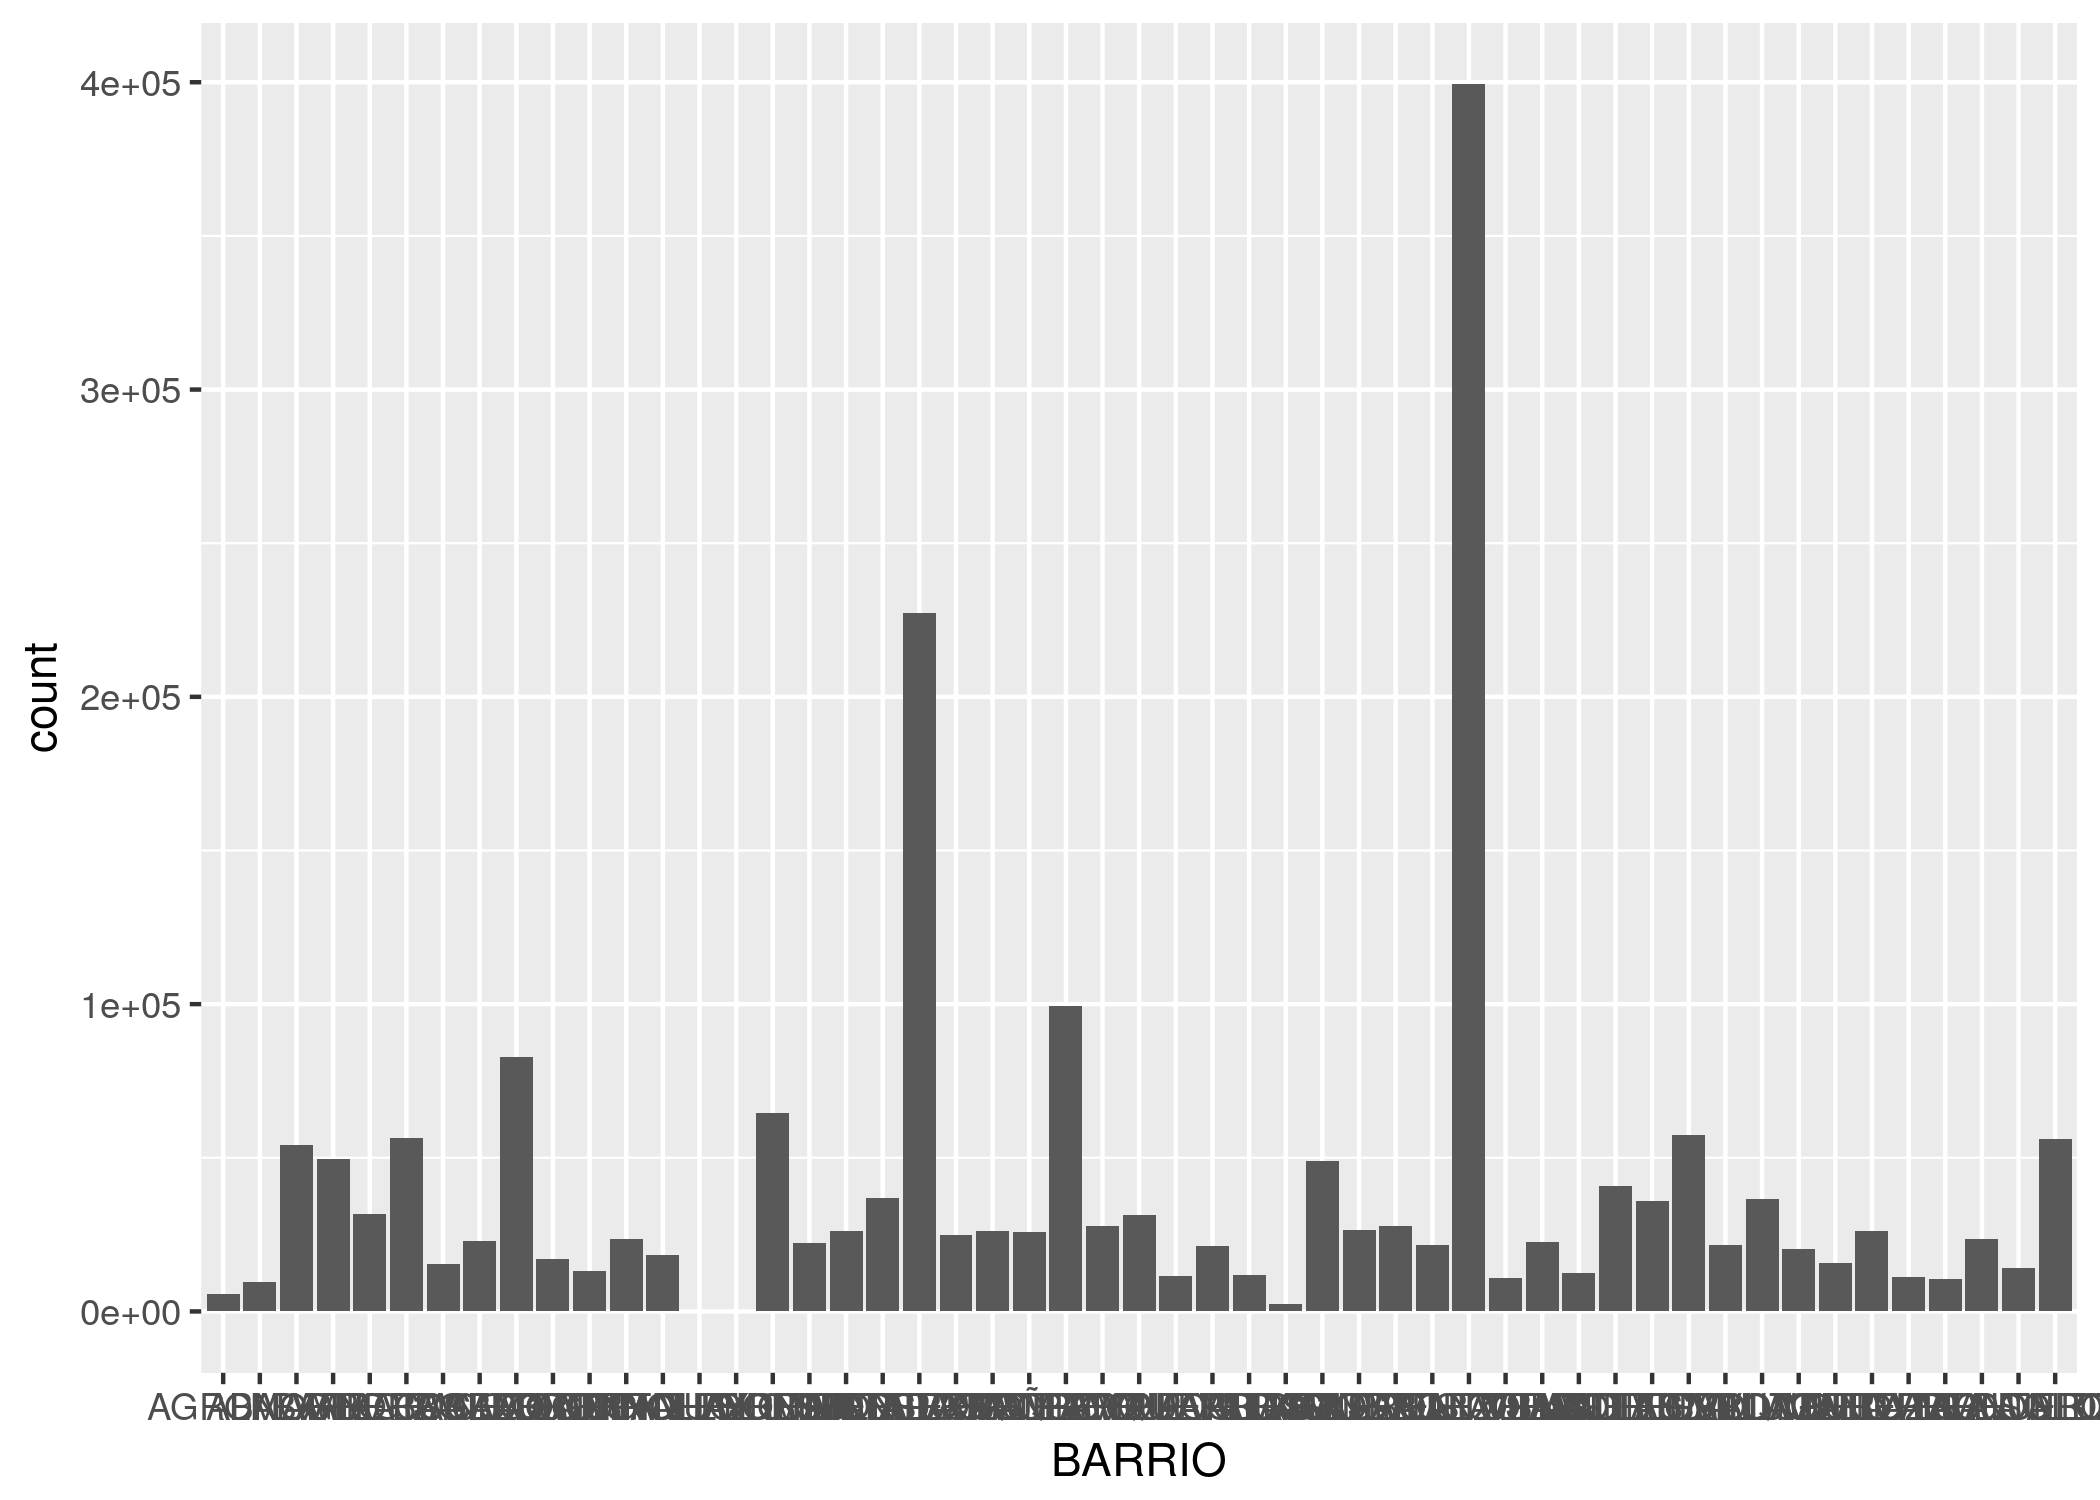
\includegraphics{ciencia_de_datos_para_gente_sociable_files/figure-latex/unnamed-chunk-95-1.pdf}

Los culpables de la anomalía son los trámites; en ninguna otra categoría
la comuna 1 se separa del resto. Sabiendo que la base de donde provienen
los datos combina información de distintos sistemas de atención, mi
interpretación es que una gran cantidad de ``TRAMITES'' proviene de
algún sistema administrativo que no guarda direcciones. Si ese fuera el
caso, parece que a todos los trámites huérfanos de origen se les asigna
una dirección en la Comuna 1 (sede histórica del Gobierno de la Ciudad)
y nosotros terminamos haciendo estas elucubraciones.

Pero valga el ejemplo para mencionar algo fundamental: por más ciencia
de datos que apliquemos, siempre vamos a llegar a un punto en que
nuestros hallazgos no tendrán sentido sin combinarlos con lo que se
llama ``conocimiento de dominio''. El conocimiento de dominio es el
saber especializado sobre el tema que estamos tratando, sea el ciclo
reproductivo de la gaviota austral o la organización administrativa del
Gobierno de la Ciudad Autónoma de Buenos Aires. Esto no debería
desanimarnos, ¡al contrario!. El análisis de datos como profesión
conlleva un constante aprendizaje sobre los más variados temas. Y a la
inversa: si somos expertos en cualquier campo, aún con un puñado de
técnicas básicas de R podemos extraer conocimiento de nuestros datos que
jamas encontraría un experto programador que no conoce el paño.

\section{Gráficos de barras}\label{graficos-de-barras}

Si hay un tipo de visualización que compite en popularidad con el
\emph{scatterplot}, son los gráficos de barras (\emph{bar charts} en
inglés). Solemos encontrarlos acompañando artículos en diarios y
revistas, sin duda porque son fáciles de leer de un vistazo. Los
gráficos de barras se usan mucho para hacer comparaciones: quién tiene
más y quién tiene menos de alguna variable continua cómo ingresos, edad,
altura o similares.

Comparemos la suma total de registros que alcanza cada barrio. Con
\texttt{geom\_bar} podemos agregar una capa de visualizacón con gráficos
de barras. Los parámetros a definir dentro de \texttt{aes()} son
\texttt{x}, donde va una variable categórica, y en forma opcional
\texttt{weight}, que indica la variable a sumar para determinar la
altura de cada barra. Si no especificamos un \texttt{weight},
simplemente se cuenta cuantas veces aparece cada categoría en el
dataframe, en la práctica un conteo o frecuencia de aparición. En
nuestro dataset cada fila incluye un período y un total de contactos
recibidos. Nosotros no estamos interesados en cuantas veces aparece cada
barrio, sino en la suma de la columna total para cada uno de ellos, así
que vamos a usar \texttt{weight\ =\ total}.

\begin{Shaded}
\begin{Highlighting}[]
\KeywordTok{ggplot}\NormalTok{(atencion_ciudadano) }\OperatorTok{+}
\StringTok{    }\KeywordTok{geom_bar}\NormalTok{(}\KeywordTok{aes}\NormalTok{(}\DataTypeTok{x =}\NormalTok{ BARRIO, }\DataTypeTok{weight =}\NormalTok{ total))}
\end{Highlighting}
\end{Shaded}

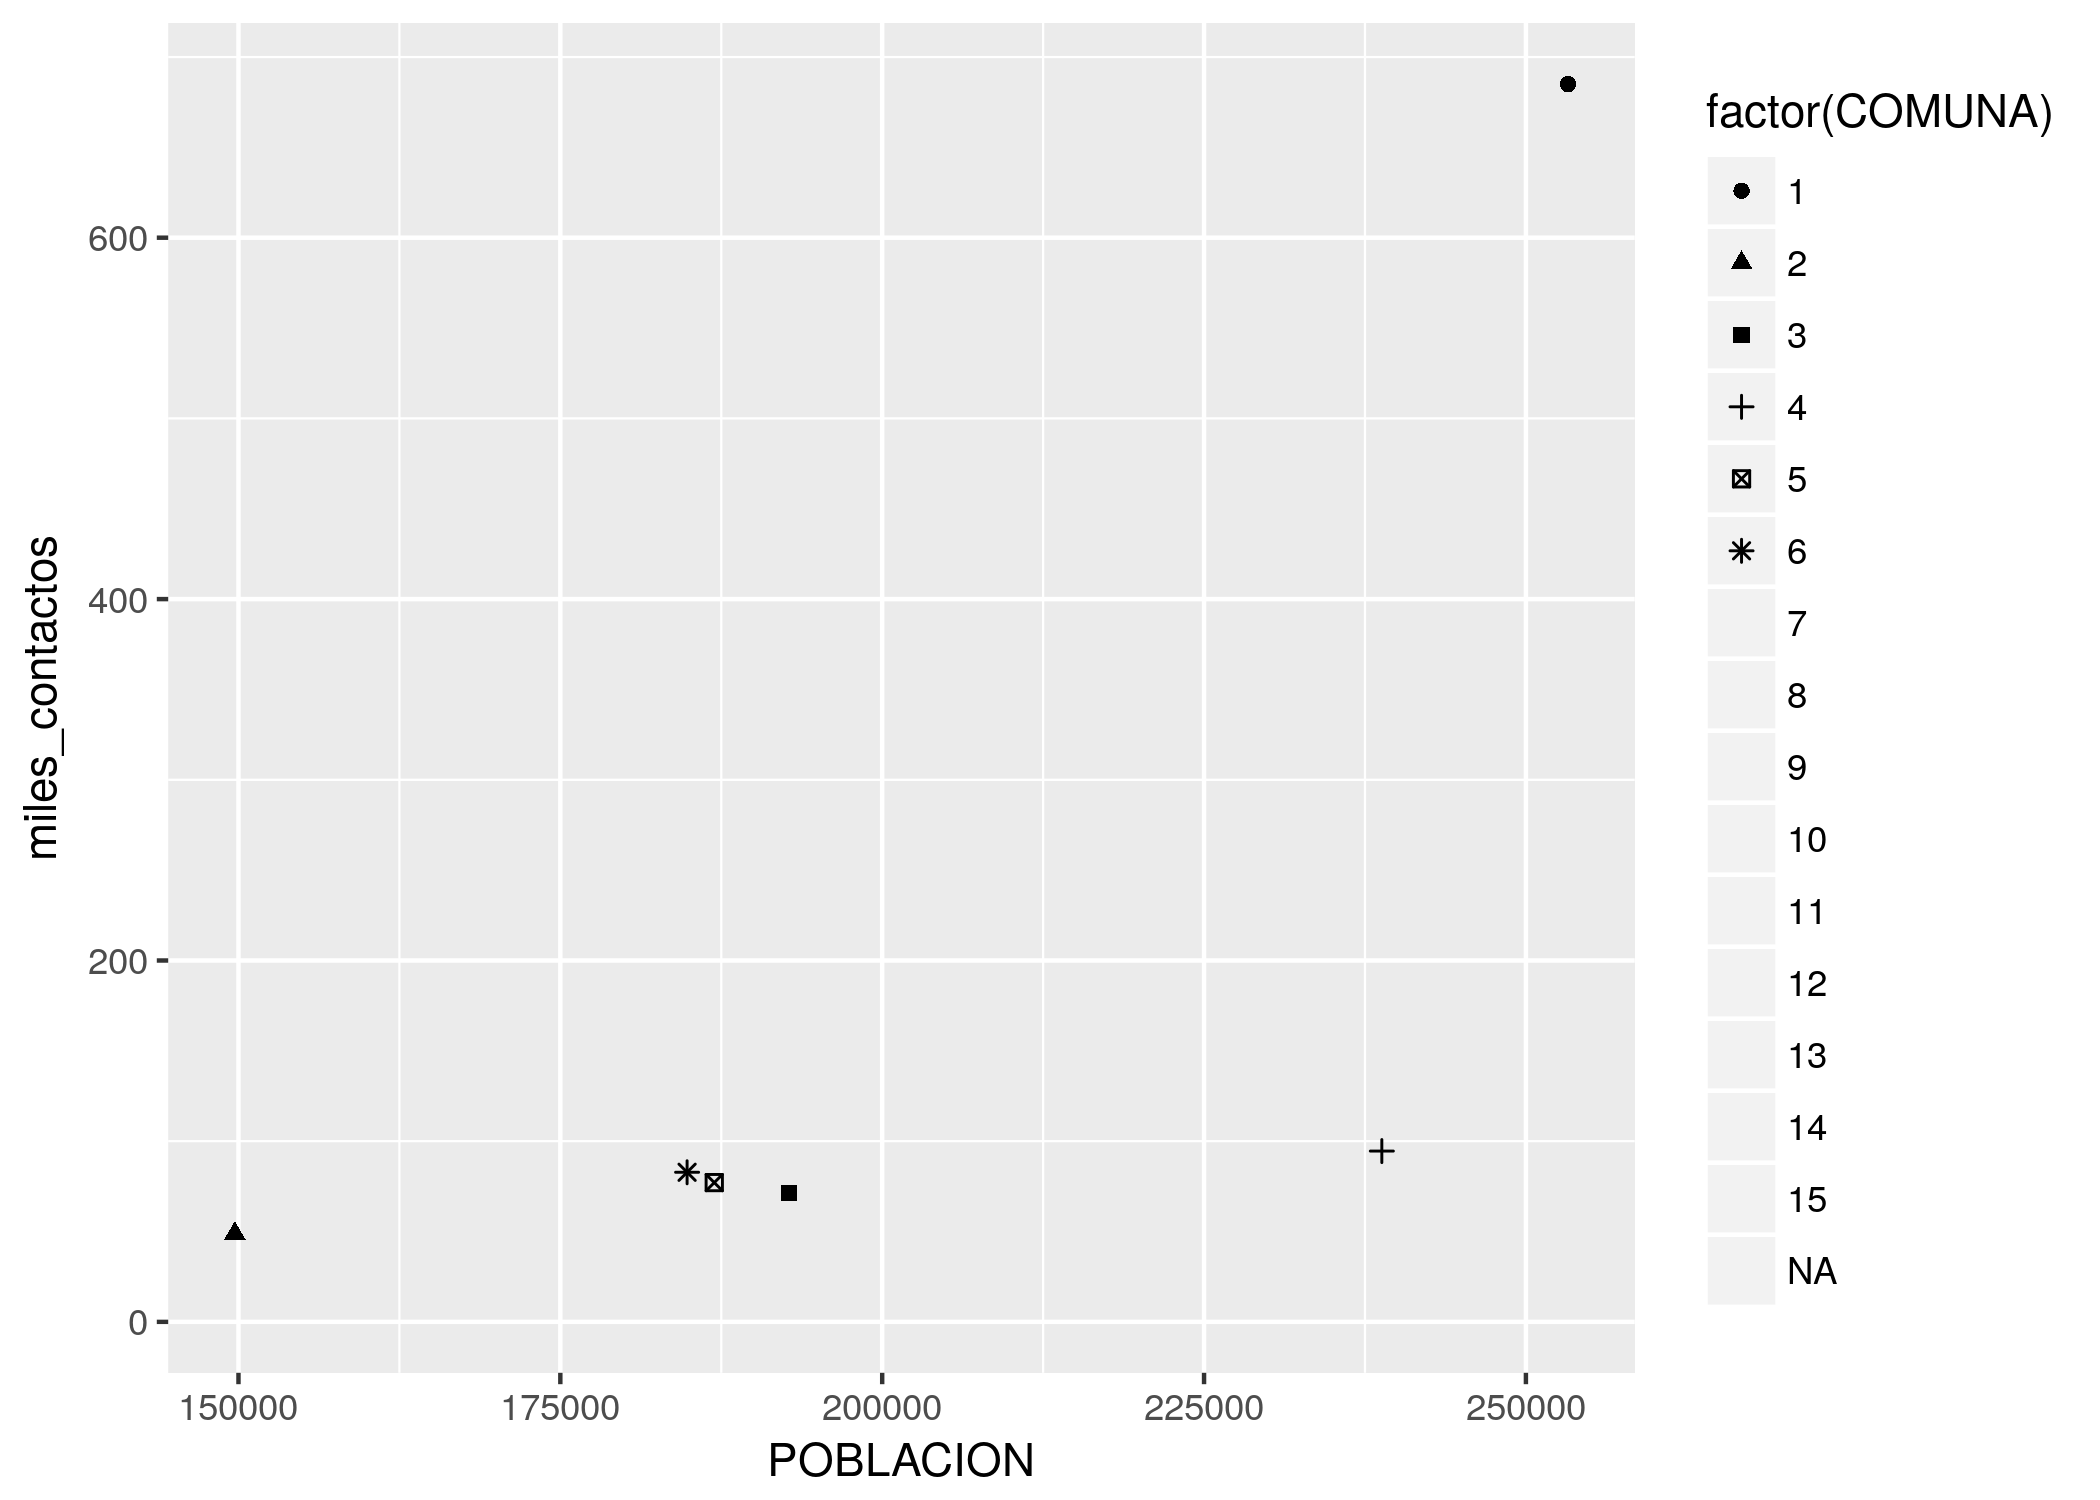
\includegraphics{ciencia_de_datos_para_gente_sociable_files/figure-latex/unnamed-chunk-96-1.pdf}

Tenemos dos problemas. El primero es que los valores en el eje de las
\texttt{y} son grandes, y R nos quiere hacer un favor expresándolos en
notación científica. La notación científica es práctica para ahorrar
espacio, pero no queda vien en visualizaciones. Para pedirle que no lo
haga mas, usamos esta función

\begin{Shaded}
\begin{Highlighting}[]
\KeywordTok{options}\NormalTok{(}\DataTypeTok{scipen =} \DecValTok{999}\NormalTok{)}
\end{Highlighting}
\end{Shaded}

y por el resto de la sesión nos libramos de la notación científica.
Listo.

El segundo problema es que los nombres de los barrios resultan del todo
ilegibles porque no tienen espacio. En un gráfico, el eje horizonatal es
un muy mal lugar para poner muchas categorías con nombre, ya que el
solapamiento se vuelve inevitable. Sería mejor tener los nombre en el
eje vertical, donde se pueden escribir uno encima del otro sin pisarse
¡La solución es invertir los ejes de de coordenadas! Sólo necesitamos
agregar \texttt{coord\_flip}:

\begin{Shaded}
\begin{Highlighting}[]
\KeywordTok{ggplot}\NormalTok{(atencion_ciudadano) }\OperatorTok{+}
\StringTok{    }\KeywordTok{geom_bar}\NormalTok{(}\KeywordTok{aes}\NormalTok{(}\DataTypeTok{x =}\NormalTok{ BARRIO, }\DataTypeTok{weight =}\NormalTok{ total)) }\OperatorTok{+}
\StringTok{    }\KeywordTok{coord_flip}\NormalTok{()}
\end{Highlighting}
\end{Shaded}

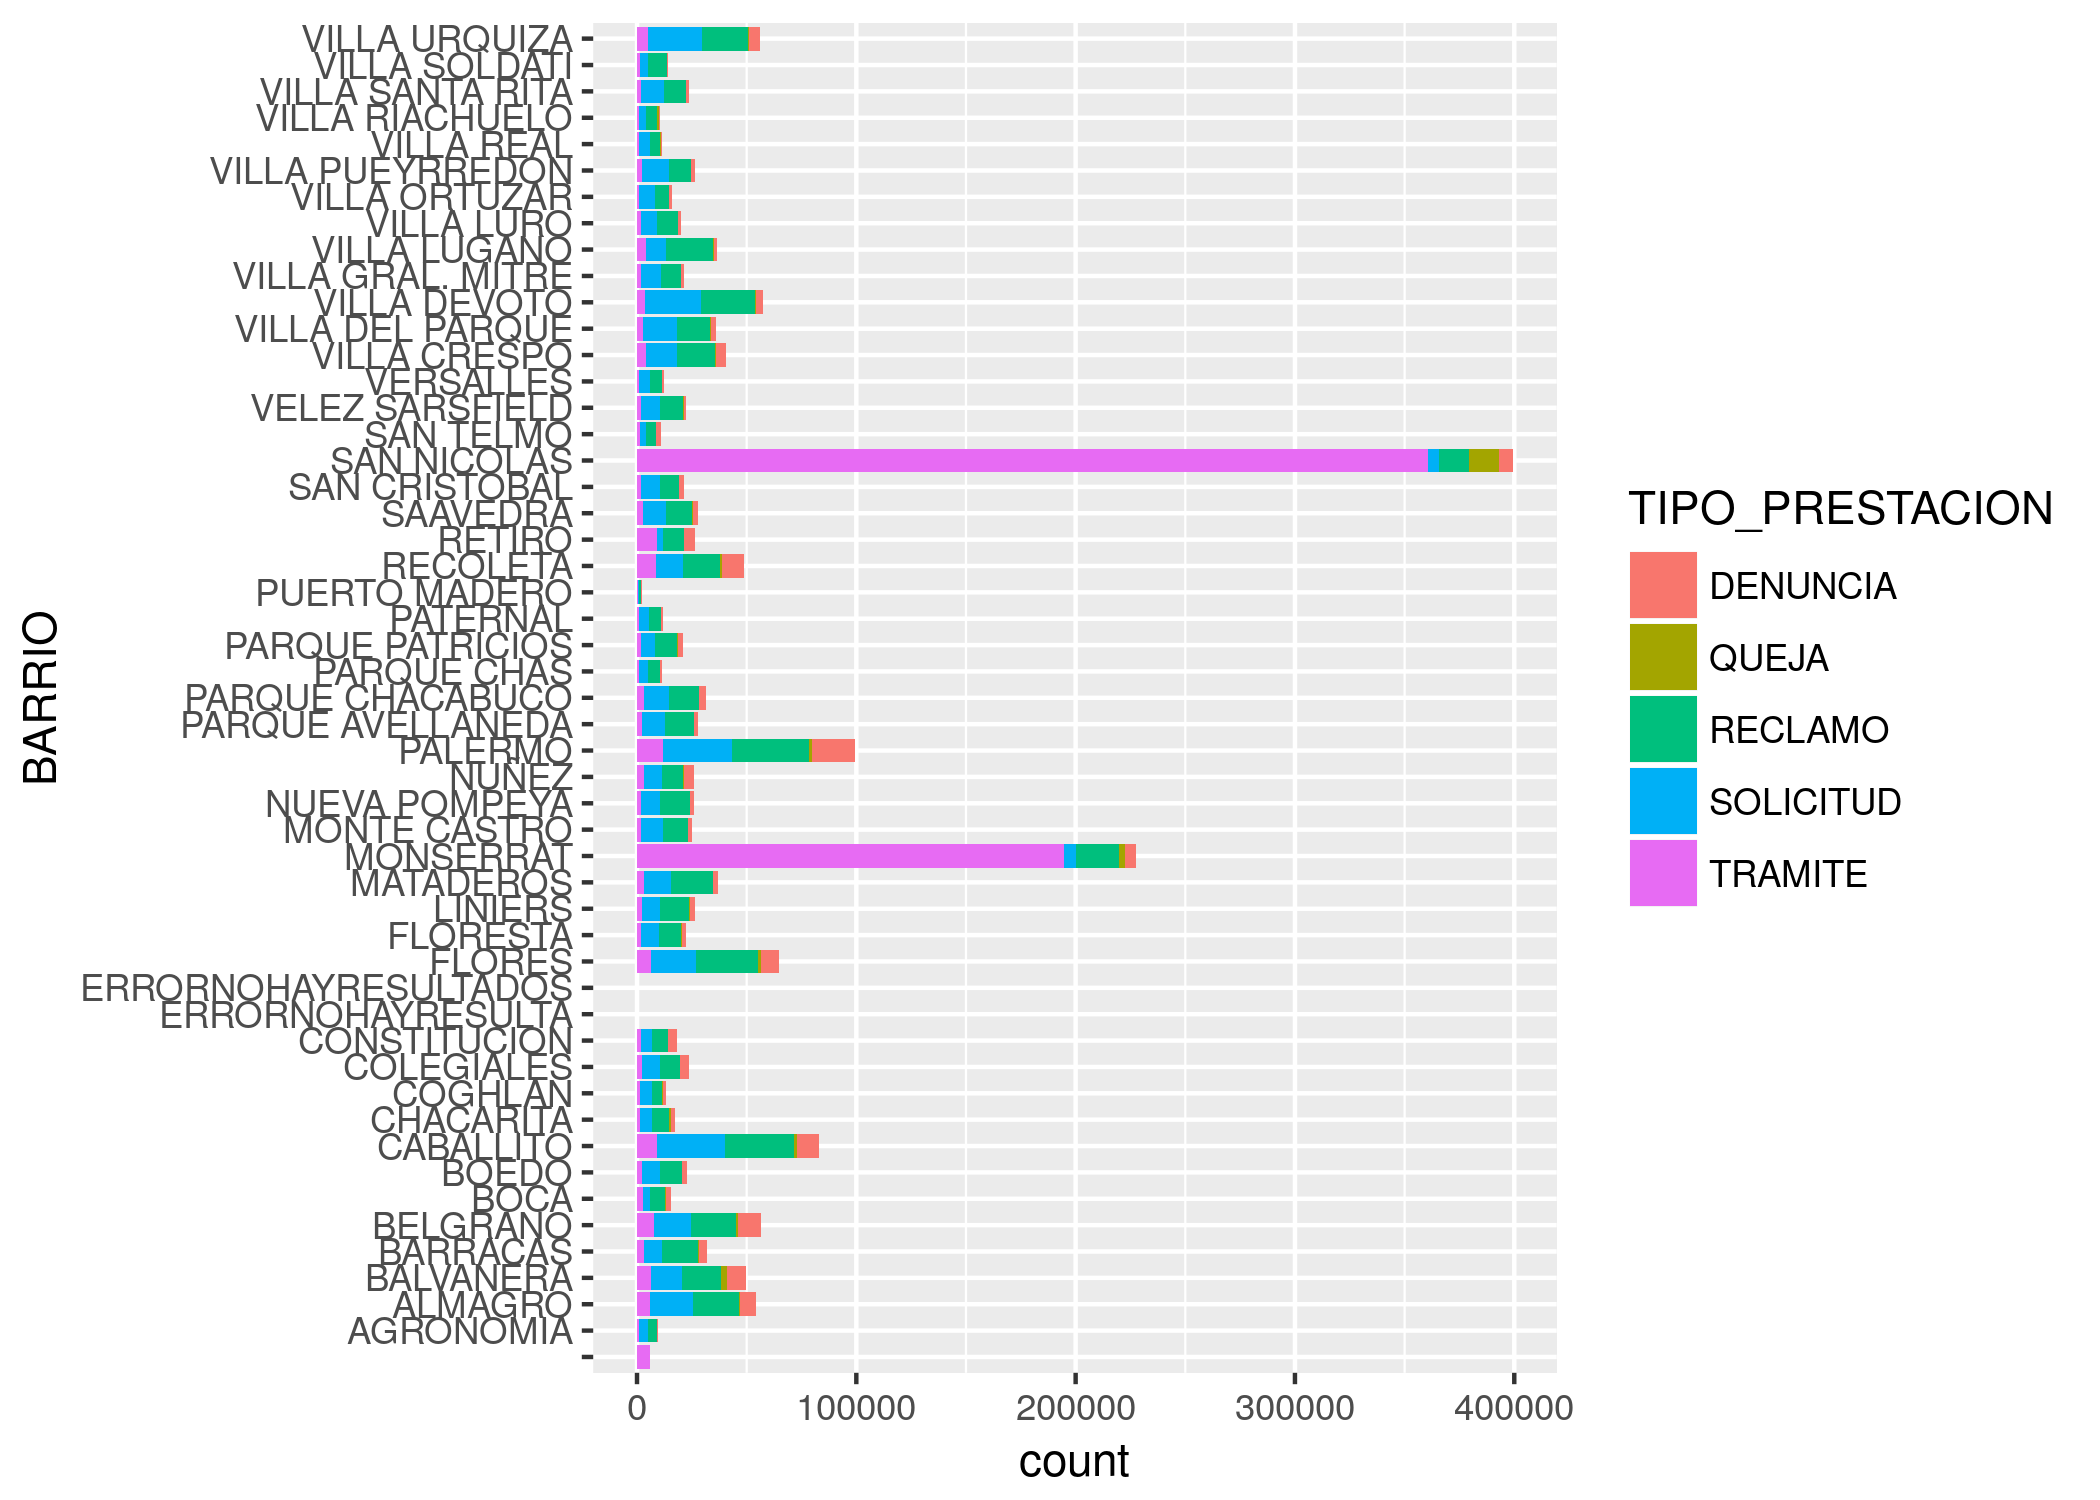
\includegraphics{ciencia_de_datos_para_gente_sociable_files/figure-latex/unnamed-chunk-98-1.pdf}

Ahora si podemos interpretar el gráfico. San Nicolás y Monserrat son los
barrios a la cabeza, lo cual no sorprende sabiendo que pertenecen a la
ya legendaria comuna 1.

Los gráficos de barras, además de comparar, también son buenos para
mostrar la composición interna de las cosas: que ``hay dentro'', que
componentes contribuye a un determinado total. Vamos a mostrar entonces
cuanto contribuye cada tipo de trámite al toal por barrio, usando el
parámetro estético \texttt{fill} (relleno). \texttt{geom\_bar} realiza
un segmentado automático de cada barra, con la proporción que le
corresponde a cada subcategoría:

\begin{Shaded}
\begin{Highlighting}[]
\KeywordTok{ggplot}\NormalTok{(atencion_ciudadano) }\OperatorTok{+}
\StringTok{    }\KeywordTok{geom_bar}\NormalTok{(}\KeywordTok{aes}\NormalTok{(}\DataTypeTok{x =}\NormalTok{ BARRIO, }\DataTypeTok{weight =}\NormalTok{ total, }\DataTypeTok{fill =}\NormalTok{ TIPO_PRESTACION)) }\OperatorTok{+}
\StringTok{    }\KeywordTok{coord_flip}\NormalTok{()}
\end{Highlighting}
\end{Shaded}

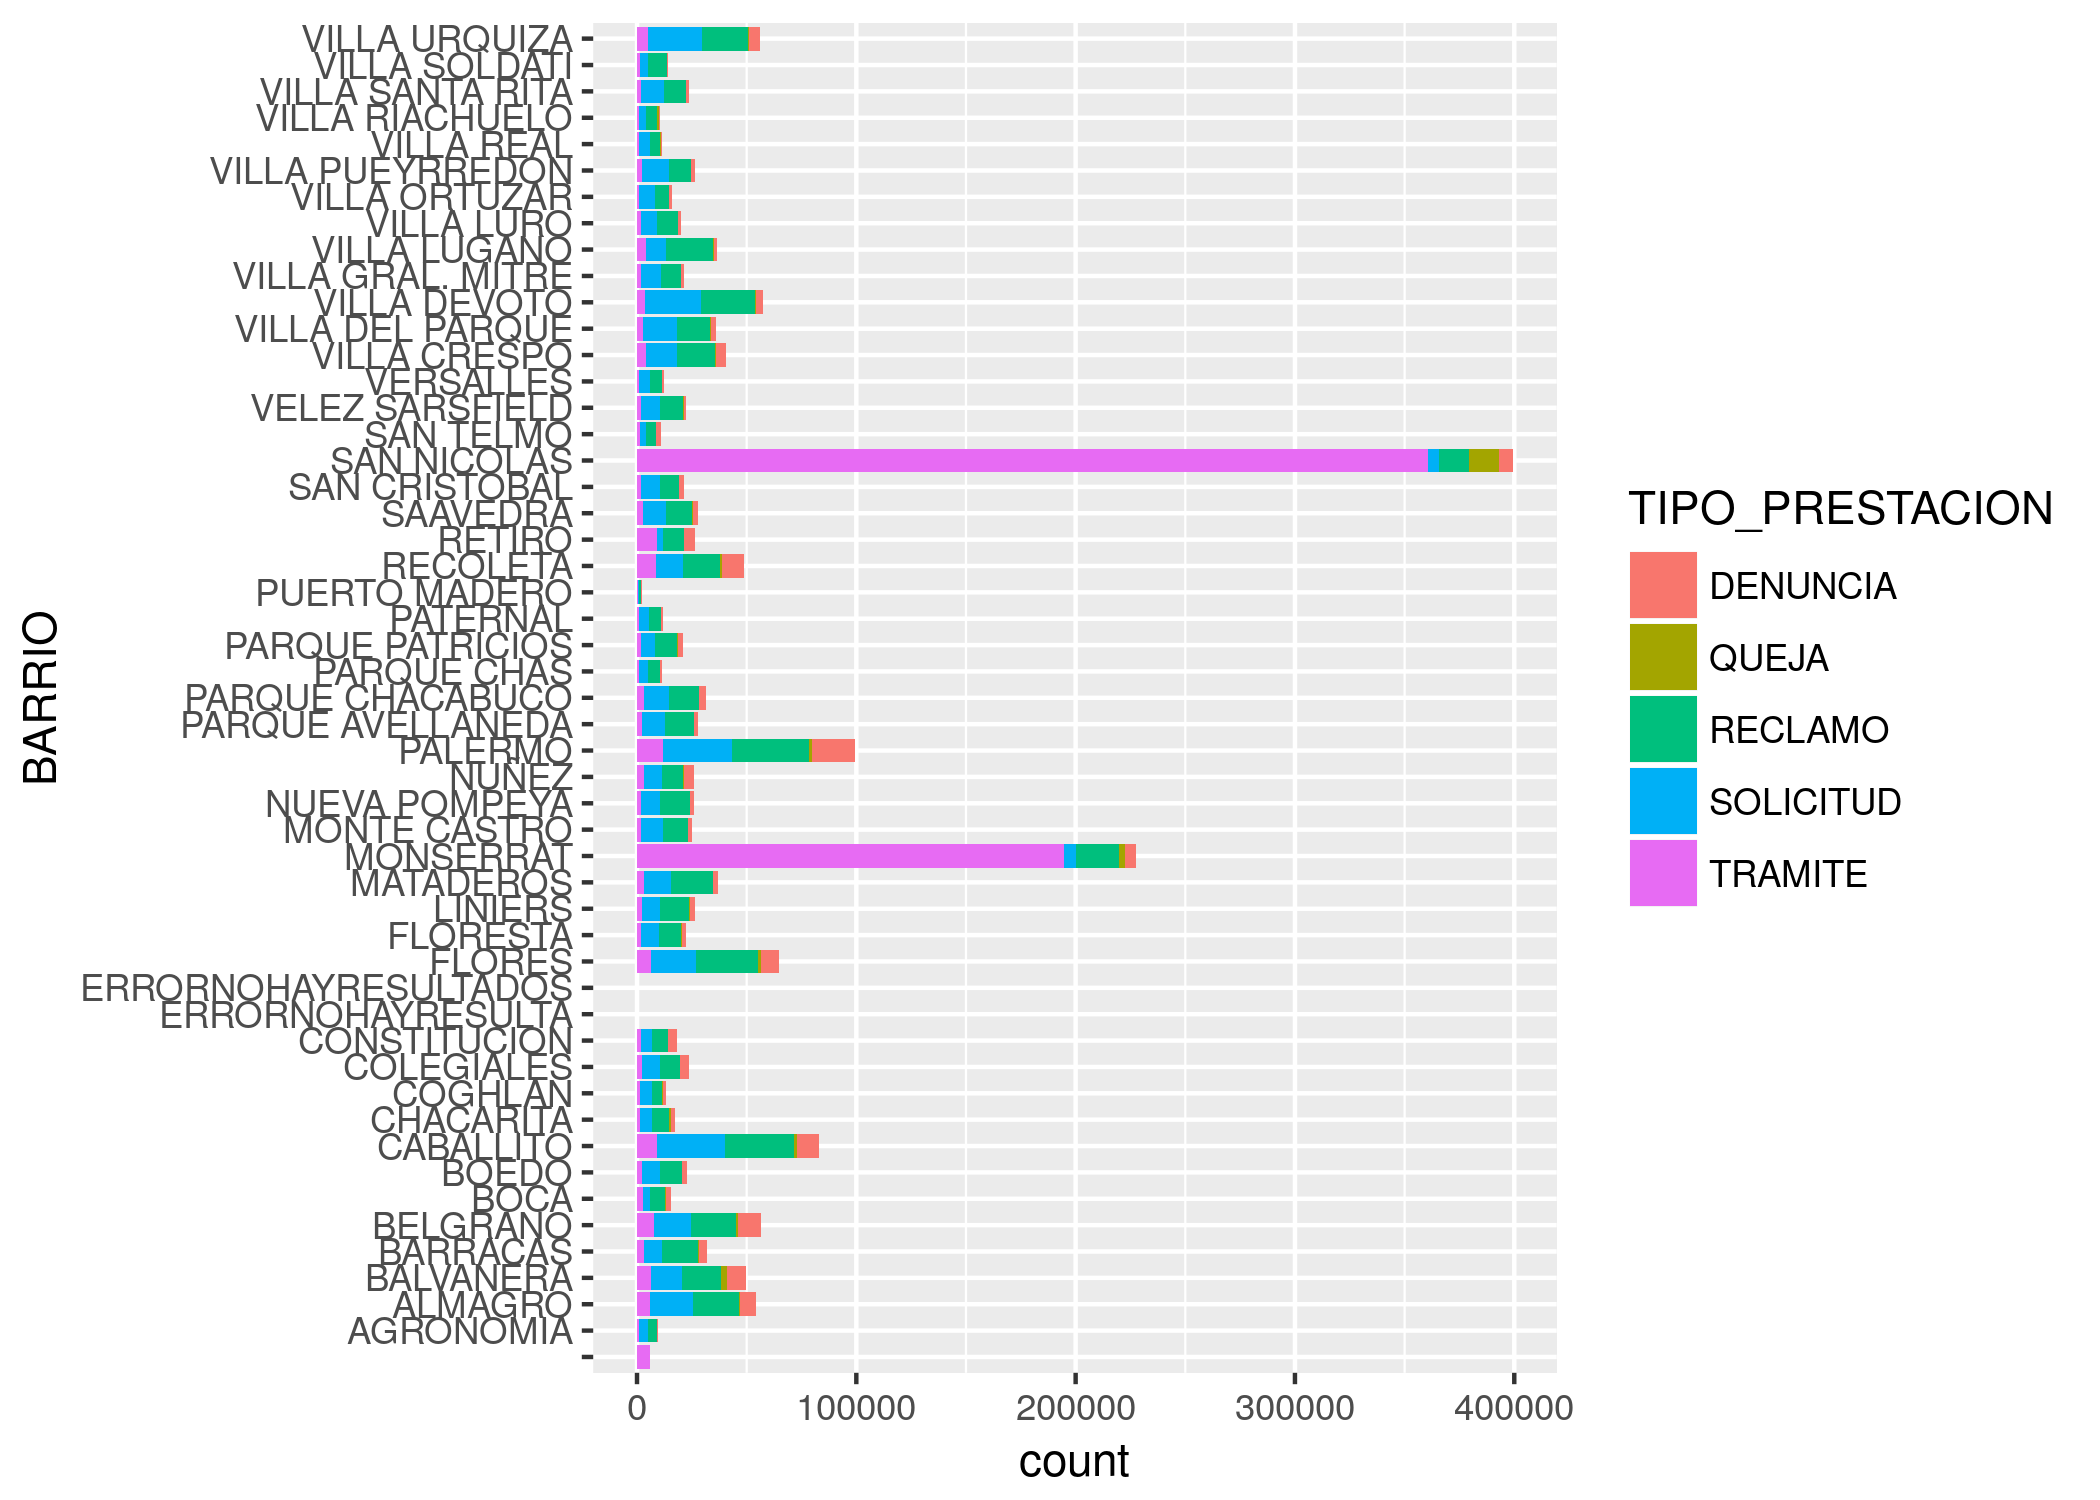
\includegraphics{ciencia_de_datos_para_gente_sociable_files/figure-latex/unnamed-chunk-99-1.pdf}

!Esos trámites otra vez! En cierto modo, estamos recorriendo las mismas
conclusiones a las que arribamos usando scatterplots, pero mostrando la
información de otra manera. De más está decirlo, hay muchas maneras de
contar las cosas.

En lugar de relleno podríamos haber usado \texttt{color}, tal como
hicimos con los puntos, pero los resultado es un poco menos legible y no
luce tan bien. La variable \texttt{color} modifica la silueta de las
barras, pero no su interior:

\begin{Shaded}
\begin{Highlighting}[]
\KeywordTok{ggplot}\NormalTok{(atencion_ciudadano) }\OperatorTok{+}
\StringTok{    }\KeywordTok{geom_bar}\NormalTok{(}\KeywordTok{aes}\NormalTok{(}\DataTypeTok{x =}\NormalTok{ BARRIO, }\DataTypeTok{weight =}\NormalTok{ total, }\DataTypeTok{color =}\NormalTok{ TIPO_PRESTACION)) }\OperatorTok{+}
\StringTok{    }\KeywordTok{coord_flip}\NormalTok{()}
\end{Highlighting}
\end{Shaded}

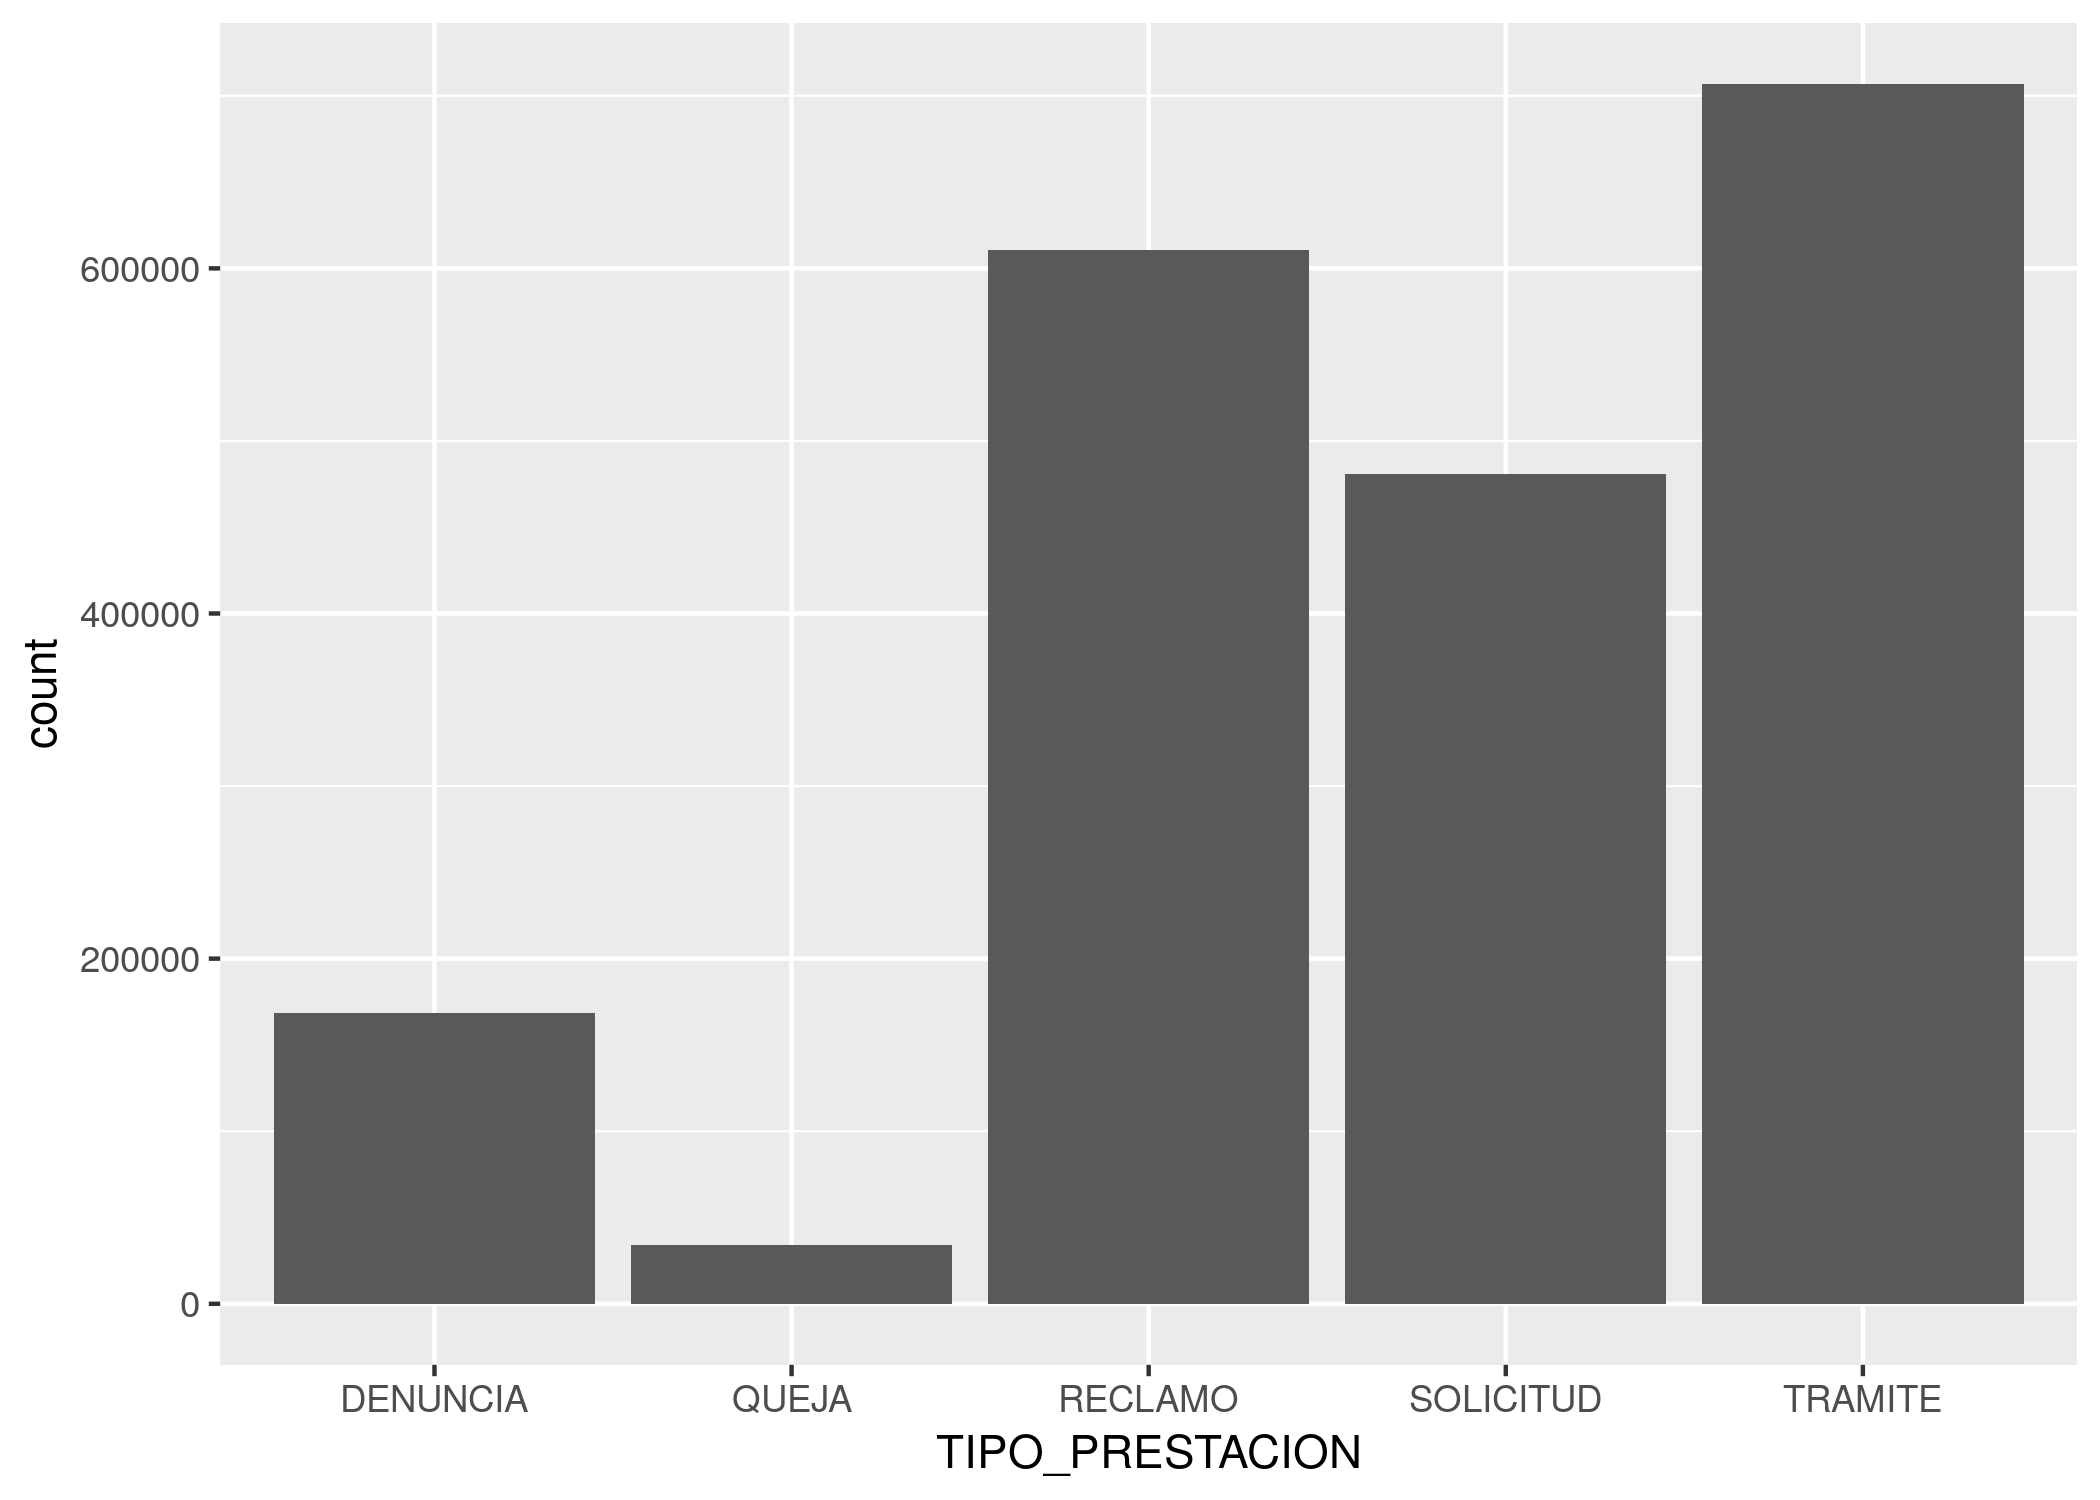
\includegraphics{ciencia_de_datos_para_gente_sociable_files/figure-latex/unnamed-chunk-100-1.pdf}

También podemos cambiar las categorías. Si qusiéramos ver el total de
registros por cada tipo de trámite:

\begin{Shaded}
\begin{Highlighting}[]
\KeywordTok{ggplot}\NormalTok{(atencion_ciudadano) }\OperatorTok{+}
\StringTok{    }\KeywordTok{geom_bar}\NormalTok{(}\KeywordTok{aes}\NormalTok{(}\DataTypeTok{x =}\NormalTok{ TIPO_PRESTACION, }\DataTypeTok{weight =}\NormalTok{ total)) }
\end{Highlighting}
\end{Shaded}

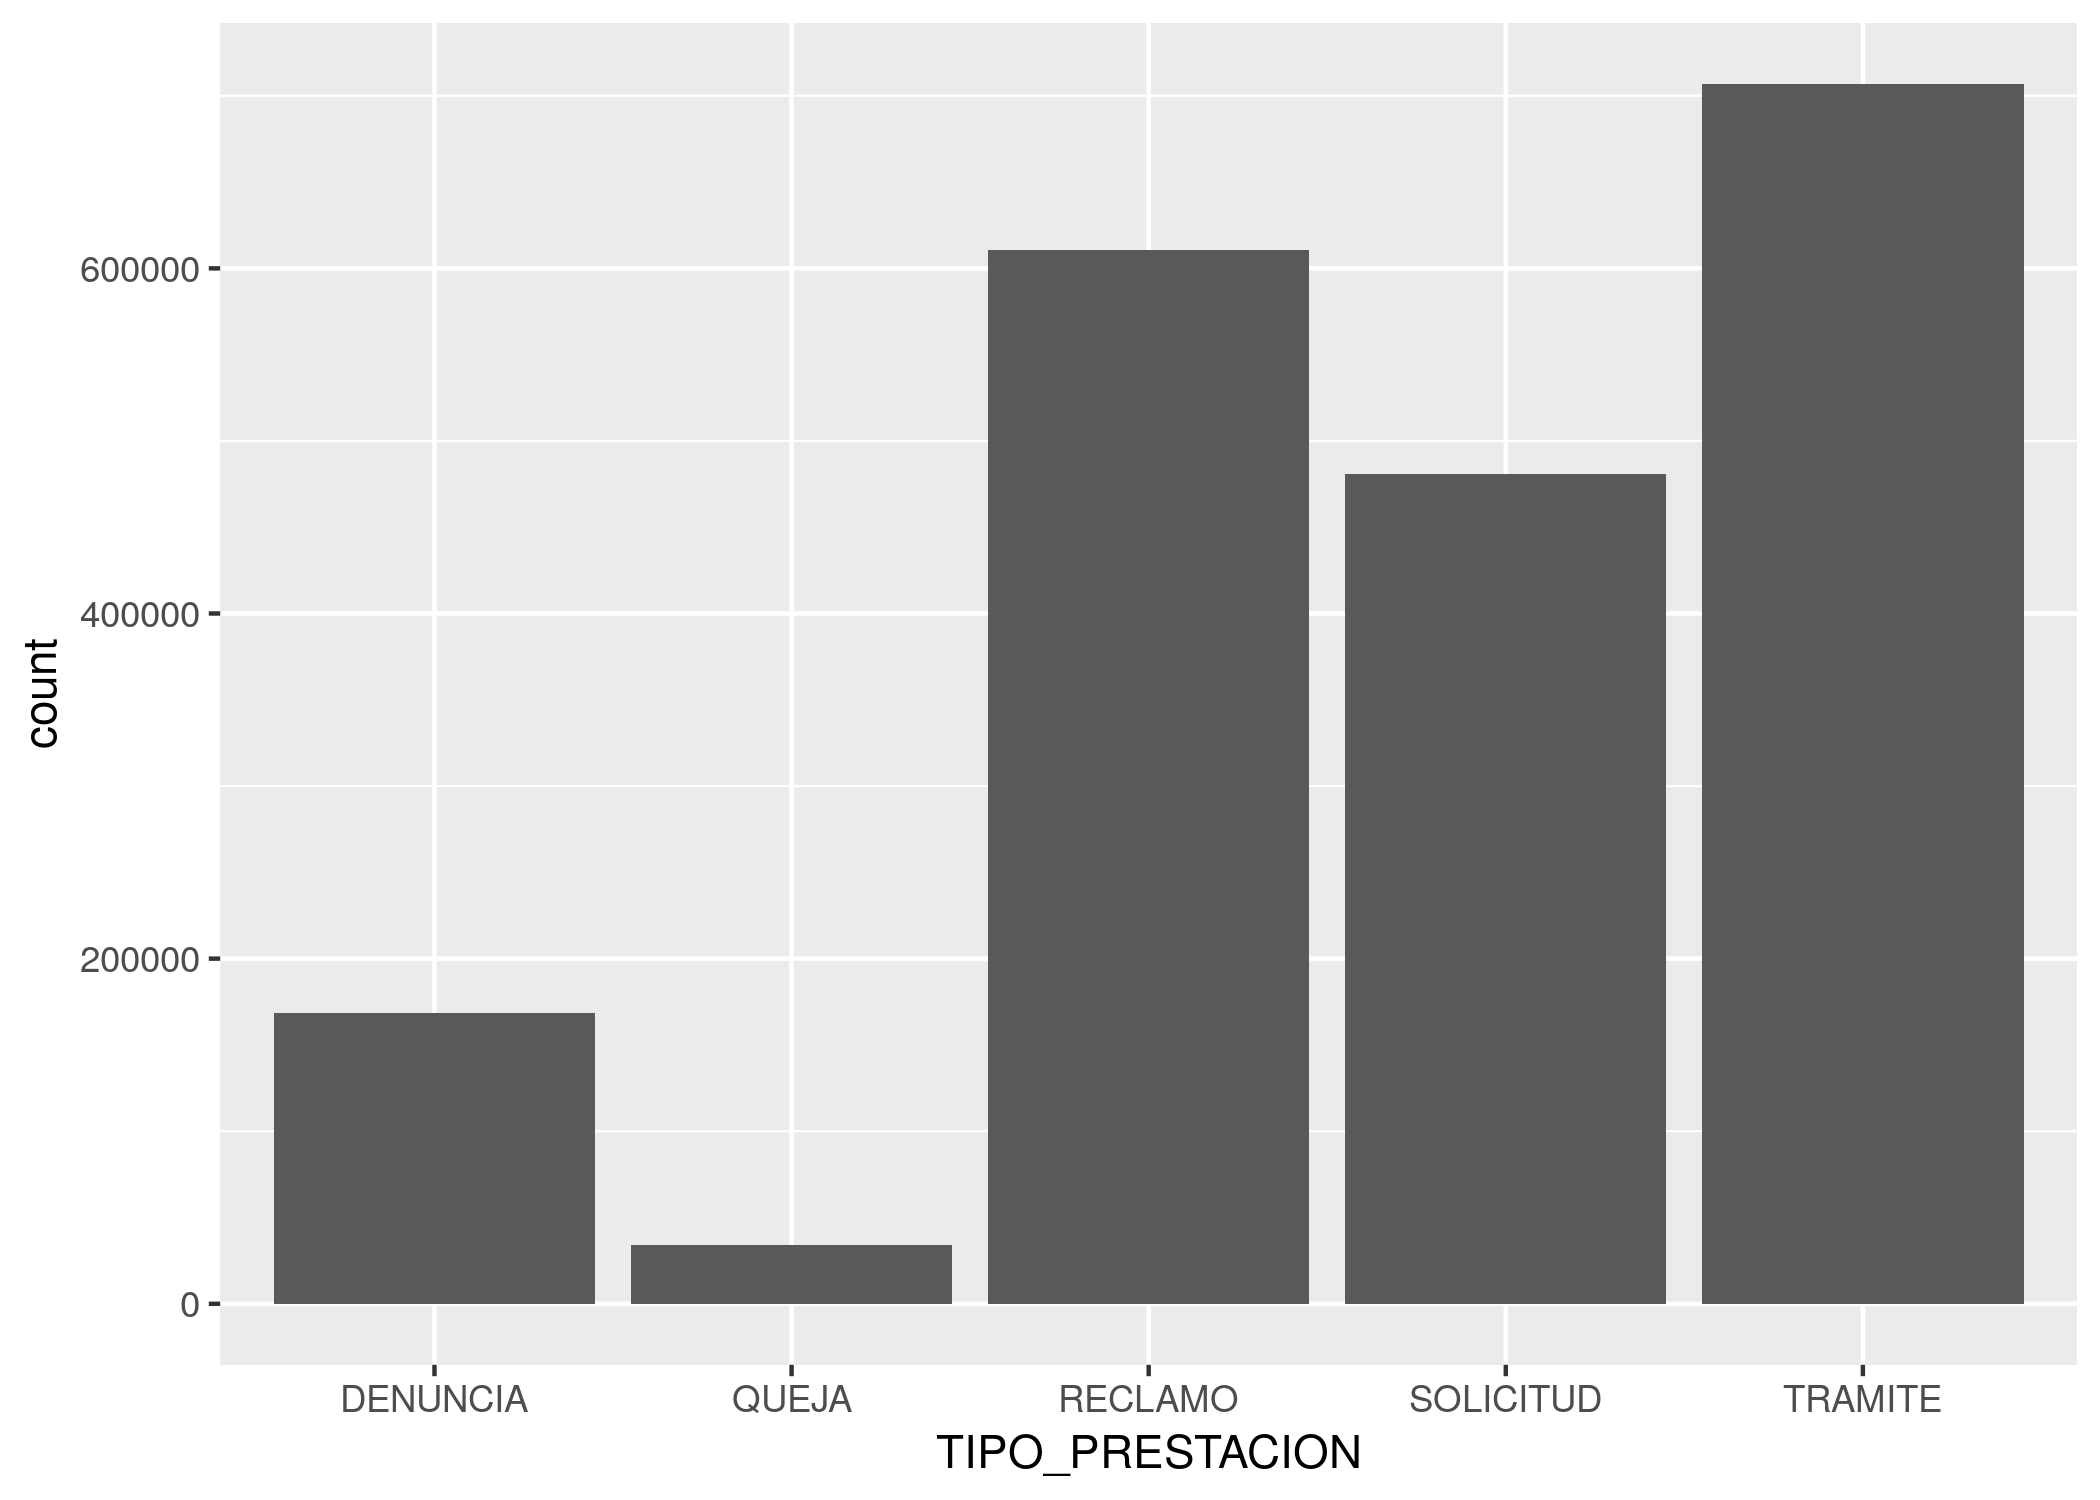
\includegraphics{ciencia_de_datos_para_gente_sociable_files/figure-latex/unnamed-chunk-101-1.pdf}

Notamos que las quejas y denuncias son eventos poco frecuentes en
comparación con las otras clases de contacto entre ciudadanos y ciudad.
En esta ocasión no recurrimos a \texttt{coord\_flip}, ya que las
categorías son pocas y tienen espacio suficiente en el eje horizontal.

¿Y si mostramos el aporte de cada barrio al total global de cada tipo de
contacto?

\begin{Shaded}
\begin{Highlighting}[]
\KeywordTok{ggplot}\NormalTok{(atencion_ciudadano) }\OperatorTok{+}
\StringTok{    }\KeywordTok{geom_bar}\NormalTok{(}\KeywordTok{aes}\NormalTok{(}\DataTypeTok{x =}\NormalTok{ TIPO_PRESTACION, }\DataTypeTok{weight =}\NormalTok{ total, }\DataTypeTok{fill =}\NormalTok{ BARRIO)) }
\end{Highlighting}
\end{Shaded}

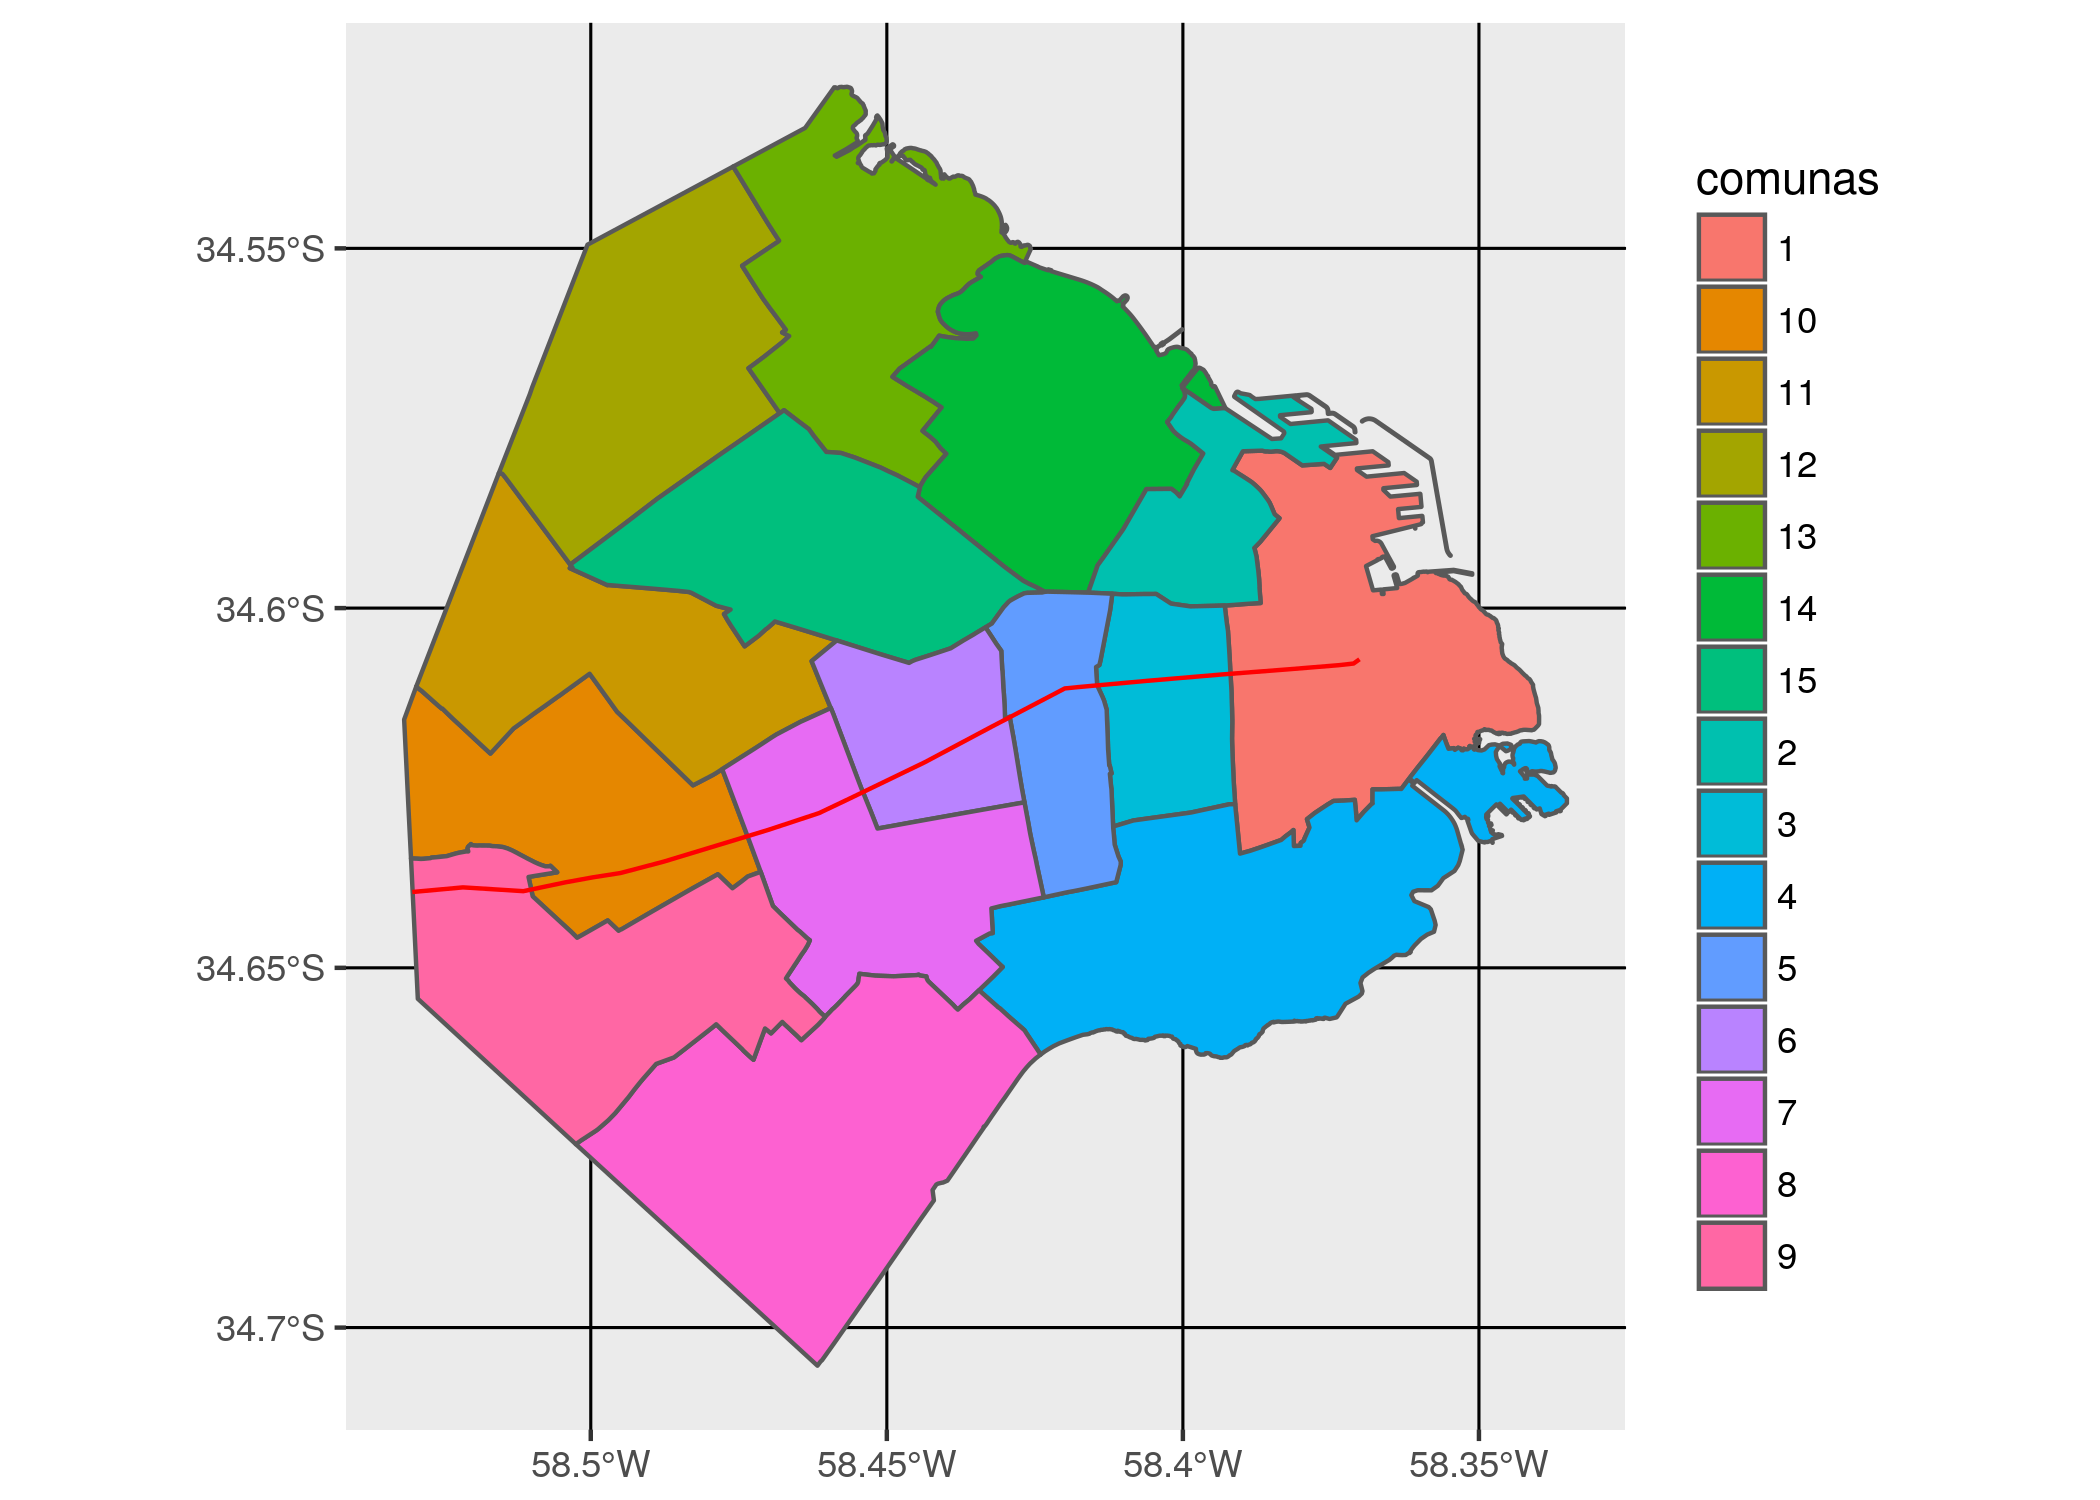
\includegraphics{ciencia_de_datos_para_gente_sociable_files/figure-latex/unnamed-chunk-102-1.pdf}

Hemos obtenido una visualización indigerible. Quizás con un facetado por
barrio\ldots{}

\begin{Shaded}
\begin{Highlighting}[]
\KeywordTok{ggplot}\NormalTok{(atencion_ciudadano) }\OperatorTok{+}
\StringTok{    }\KeywordTok{geom_bar}\NormalTok{(}\KeywordTok{aes}\NormalTok{(}\DataTypeTok{x =}\NormalTok{ TIPO_PRESTACION, }\DataTypeTok{weight =}\NormalTok{ total)) }\OperatorTok{+}
\StringTok{    }\KeywordTok{facet_wrap}\NormalTok{(}\OperatorTok{~}\NormalTok{BARRIO)}
\end{Highlighting}
\end{Shaded}

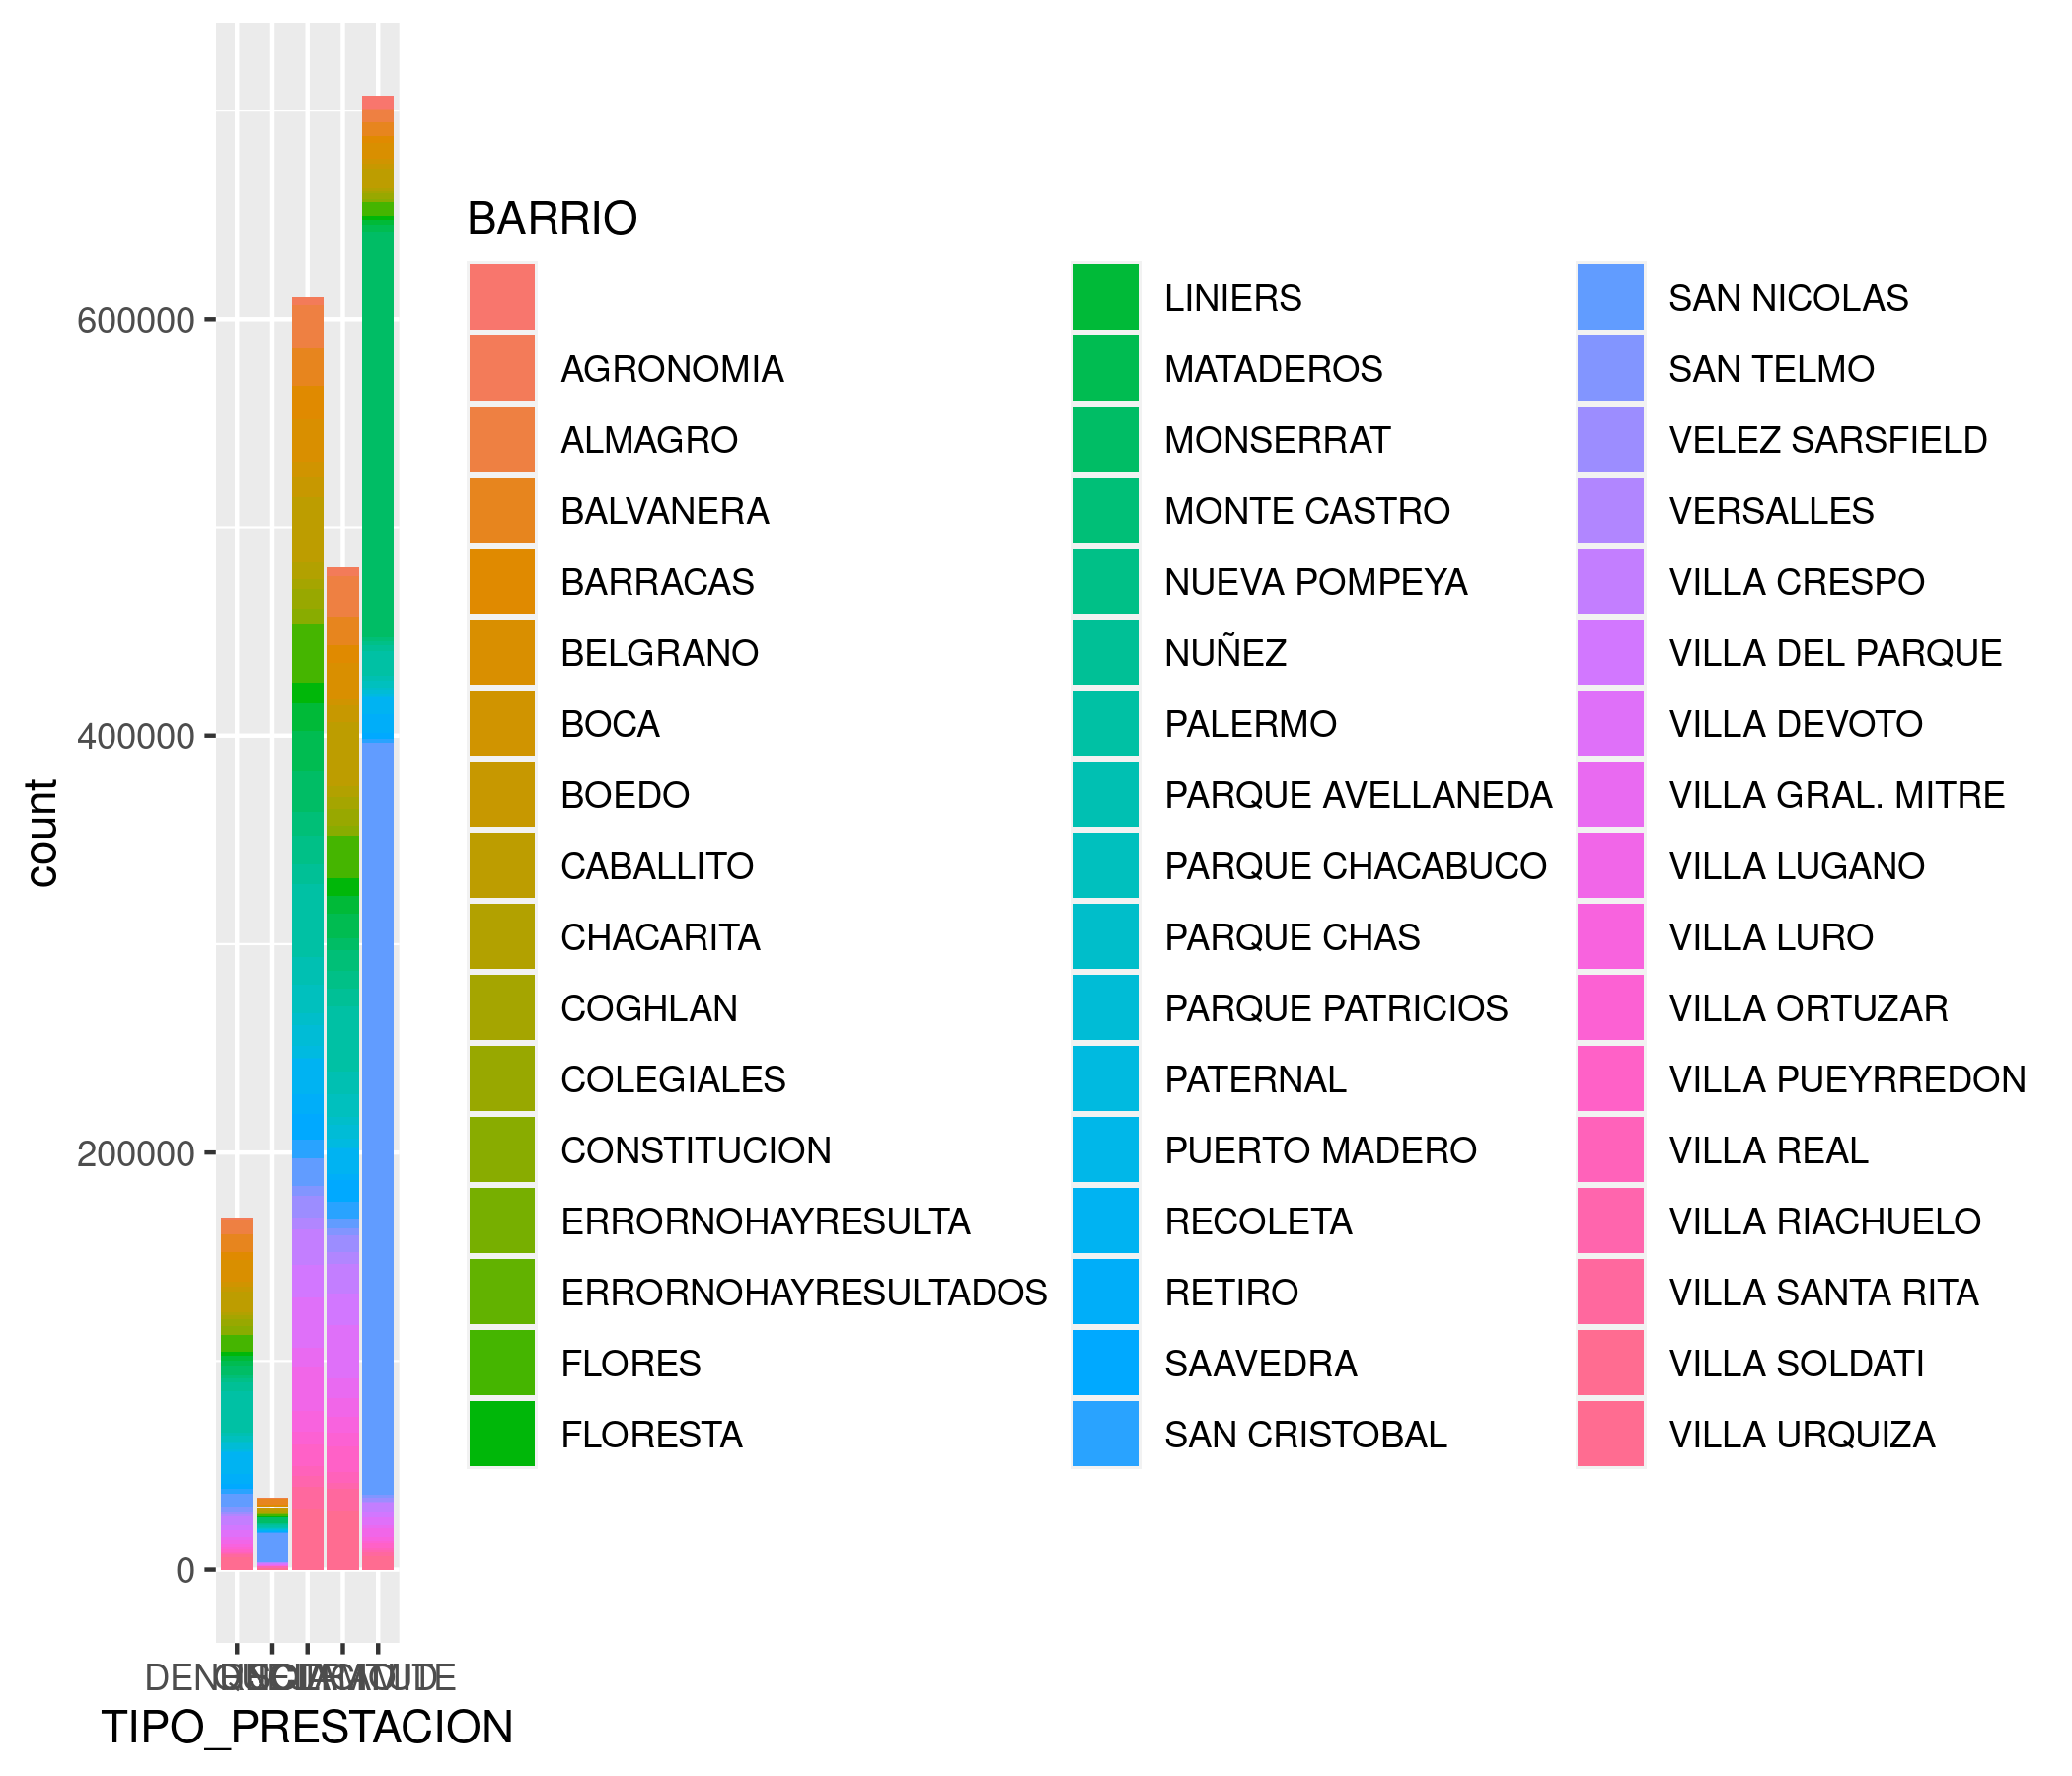
\includegraphics{ciencia_de_datos_para_gente_sociable_files/figure-latex/unnamed-chunk-103-1.pdf}

Esta opción es un poco mejor, ya que al menos permite identificar pronto
los barrios salientes, y discernir diferencias generales si se la mira
con paciencia. Una visualización tan densa en información puede resultar
ideal para ``uso personal'', explorando de forma rápida datos con los
que estamos familiarizados, pero es poco recomendable para compartir con
otros.

En general, para evitar la confusión asociada a variables con docenas de
categorías se busca simplificar definiendo menos grupos. Por ejemplo,
como hicimos al comienzo al separar por comunas, que son sólo quince, en
lugar de por barrios.

\section{Histogramas}\label{histogramas}

Los histogramas son usados para mostrar la \emph{distribución} de una
variable continua. El histograma permite decir si los valores que toma
cada observación se agrupan en torno a un valor ``típico'' o medio -como
en el caso de la llamada \emph{distribución normal}-, o en torno a dos
valores frecuentes (\emph{distribución bimodal}), o con dispersión sin
picos ni valles, donde no hay valores típicos ni atípicos -
\emph{distribución uniforme}.

Por ejemplo, analicemos la distribución de resgistros mensuales (la
columna PERIODO en nuestro datset representa el lapso de un mes).
Tenemos que agrupar por mes, y hacer un resumen (\texttt{summarise()})
que extraiga el gran total:

\begin{Shaded}
\begin{Highlighting}[]
\NormalTok{contactos_por_mes <-}\StringTok{ }\NormalTok{atencion_ciudadano }\OperatorTok\StringTok{ }
\StringTok{    }\KeywordTok{group_by}\NormalTok{(PERIODO) }\OperatorTok\StringTok{ }
\StringTok{    }\KeywordTok{summarise}\NormalTok{(}\DataTypeTok{gran_total =} \KeywordTok{sum}\NormalTok{(total))}

\KeywordTok{head}\NormalTok{(contactos_por_mes)}
\end{Highlighting}
\end{Shaded}

\begin{verbatim}
## # A tibble: 6 x 2
##   PERIODO gran_total
##     <int>      <int>
## 1  201301      43826
## 2  201302      43666
## 3  201303      47405
## 4  201304      50768
## 5  201305      52761
## 6  201306      48344
\end{verbatim}

Hacer un histograma es simple con \texttt{geom\_histogram()}: sólo hay
que elegir una variable y asignarla a las \texttt{x}.

\begin{Shaded}
\begin{Highlighting}[]
\KeywordTok{ggplot}\NormalTok{(contactos_por_mes) }\OperatorTok{+}\StringTok{ }
\StringTok{    }\KeywordTok{geom_histogram}\NormalTok{(}\KeywordTok{aes}\NormalTok{(}\DataTypeTok{x =}\NormalTok{ gran_total))}
\end{Highlighting}
\end{Shaded}

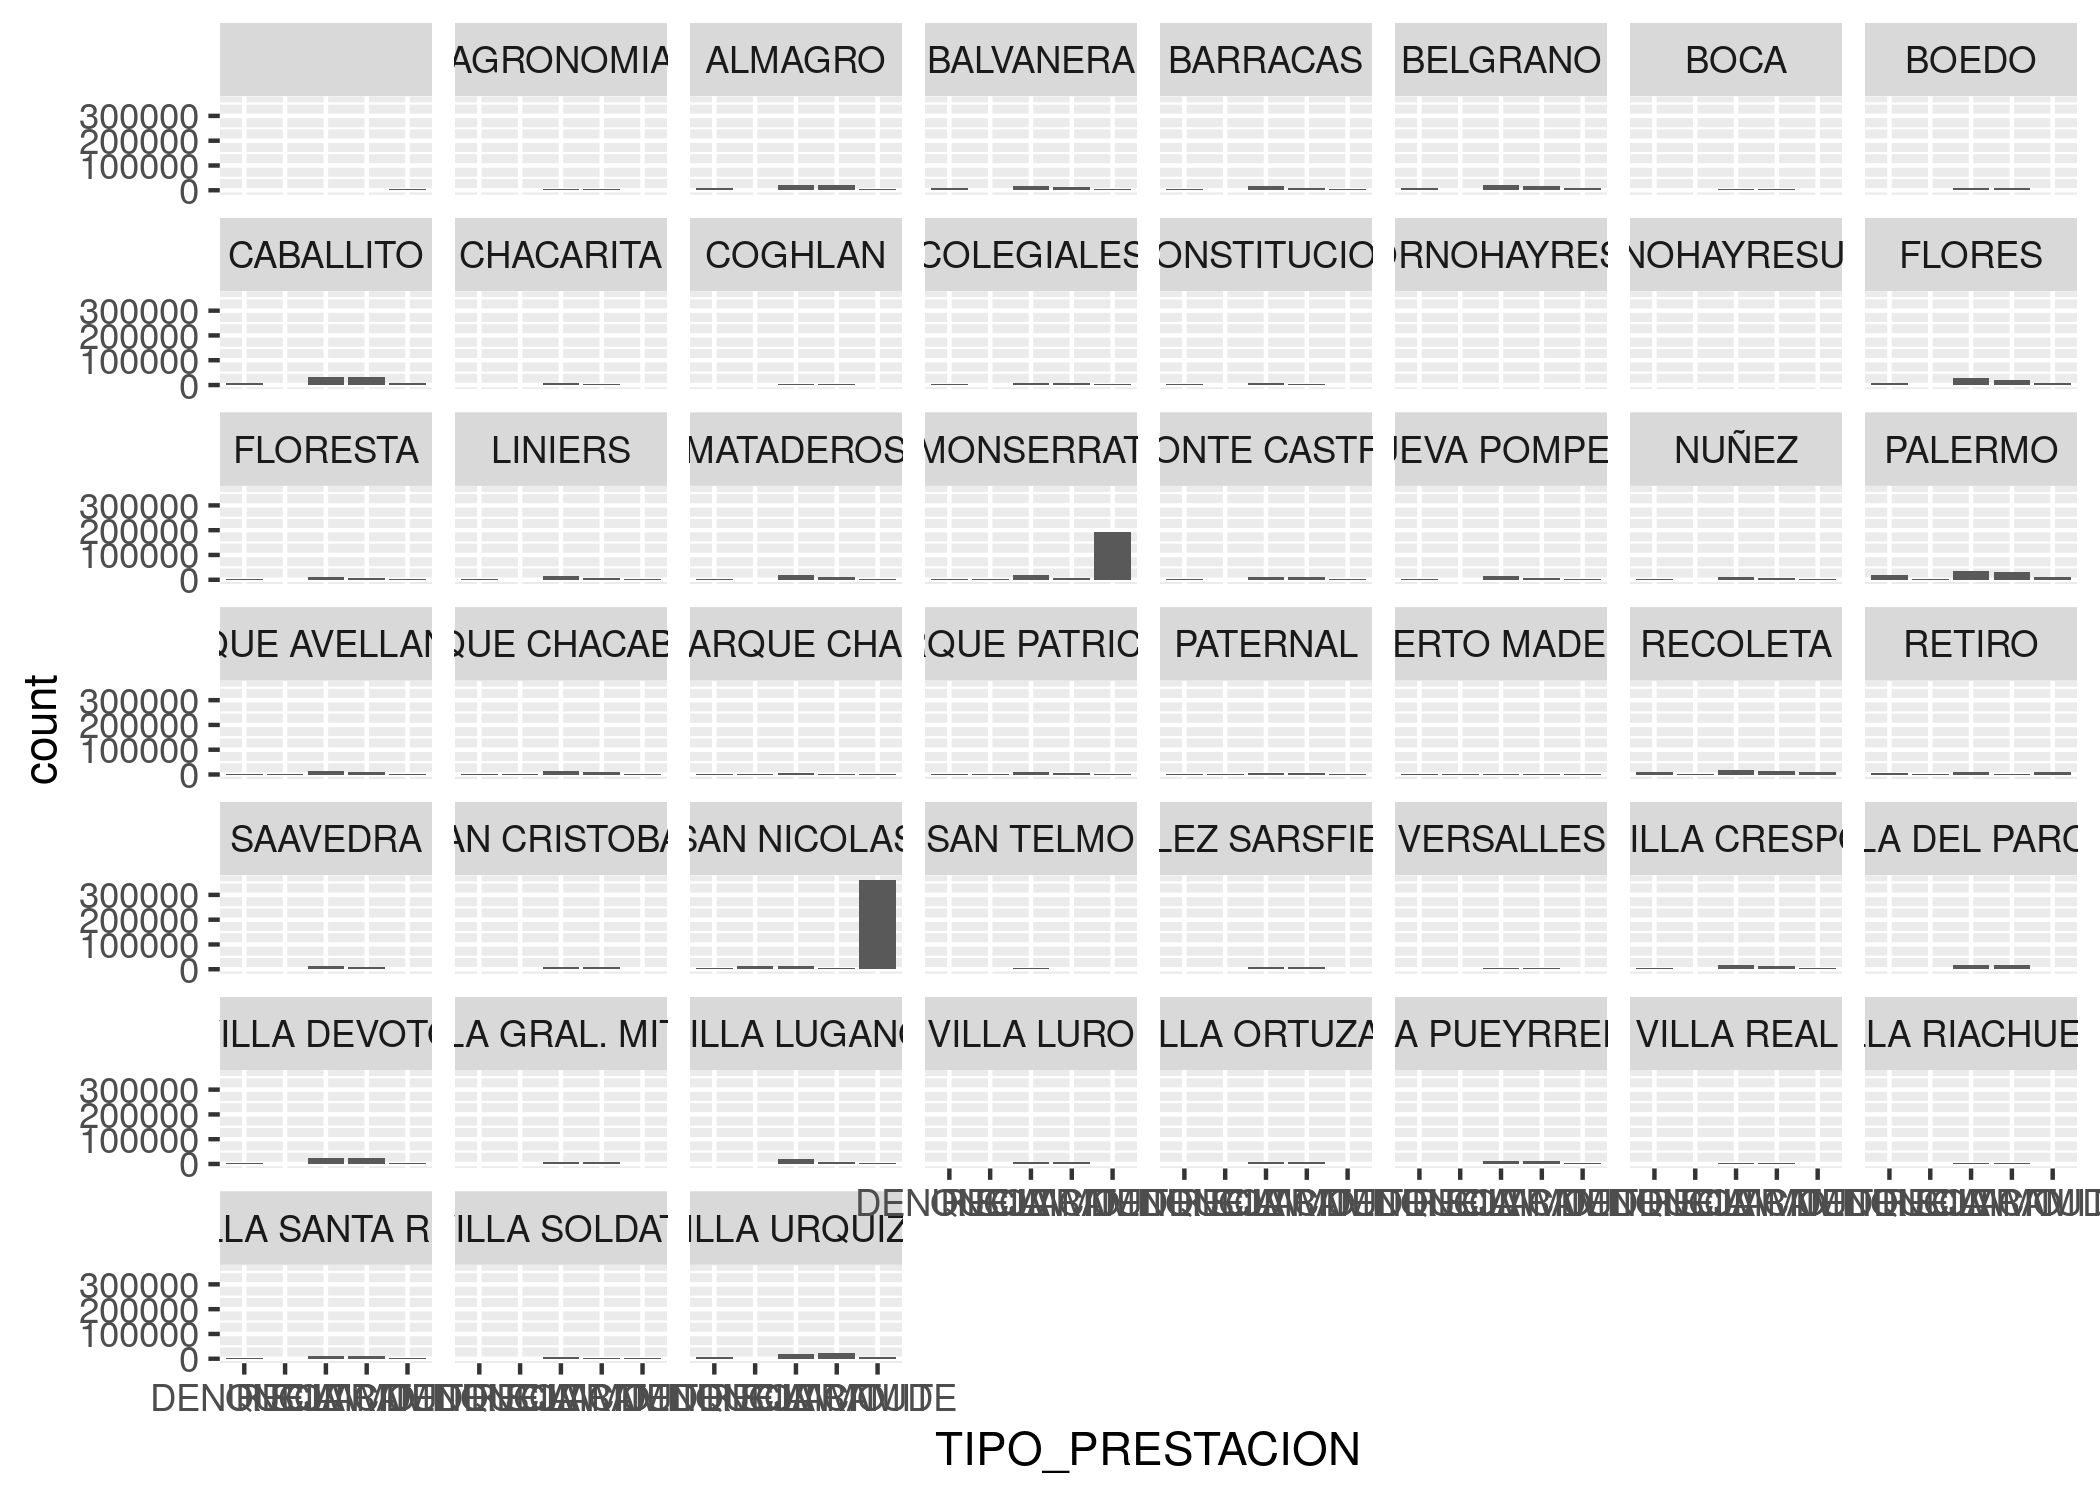
\includegraphics{ciencia_de_datos_para_gente_sociable_files/figure-latex/unnamed-chunk-105-1.pdf}

\texttt{geom\_histogram()} divide el rango de valores en una cantidad
arbitraria de segmentos iguales (``bins'' en inglés) y cuenta cuantas
observaciones caen en cada uno, cantidad que se representa con la altura
de la columna en el eje de las \texttt{y}.

En nuestro ejemplo, vemos que un mes mes en el que la cantidad de
resgitros tiende a agurparse en torno a un valor típico de poco más de
60.000 por mes. En apenas un caso hubo mennos de 40.000 o más de 80.000

No sería raro que la agregación qeu hicimos nos oculte patrones en los
datos. Que pasa si contamos los registros por mes y por tipo de
contacto, y mostramso los histogramas mensuales en facetado por tipo?

Hacemos el agrupado y sumario de rigor

\begin{Shaded}
\begin{Highlighting}[]
\NormalTok{contactos_por_mes_y_tipo <-}\StringTok{ }\NormalTok{atencion_ciudadano }\OperatorTok\StringTok{ }
\StringTok{    }\KeywordTok{group_by}\NormalTok{(PERIODO, TIPO_PRESTACION) }\OperatorTok\StringTok{ }
\StringTok{    }\KeywordTok{summarise}\NormalTok{(}\DataTypeTok{gran_total =} \KeywordTok{sum}\NormalTok{(total))}

\KeywordTok{head}\NormalTok{(contactos_por_mes_y_tipo)}
\end{Highlighting}
\end{Shaded}

\begin{verbatim}
## # A tibble: 6 x 3
## # Groups:   PERIODO [2]
##   PERIODO TIPO_PRESTACION gran_total
##     <int> <fct>                <int>
## 1  201301 DENUNCIA              2740
## 2  201301 QUEJA                  889
## 3  201301 RECLAMO              16011
## 4  201301 SOLICITUD            15325
## 5  201301 TRAMITE               8861
## 6  201302 DENUNCIA              2463
\end{verbatim}

y creamos el facetado como ya sabemos:

\begin{Shaded}
\begin{Highlighting}[]
\KeywordTok{ggplot}\NormalTok{(contactos_por_mes_y_tipo) }\OperatorTok{+}\StringTok{ }
\StringTok{    }\KeywordTok{geom_histogram}\NormalTok{(}\KeywordTok{aes}\NormalTok{(}\DataTypeTok{x =}\NormalTok{ gran_total)) }\OperatorTok{+}
\StringTok{    }\KeywordTok{facet_wrap}\NormalTok{(}\OperatorTok{~}\NormalTok{TIPO_PRESTACION)}
\end{Highlighting}
\end{Shaded}

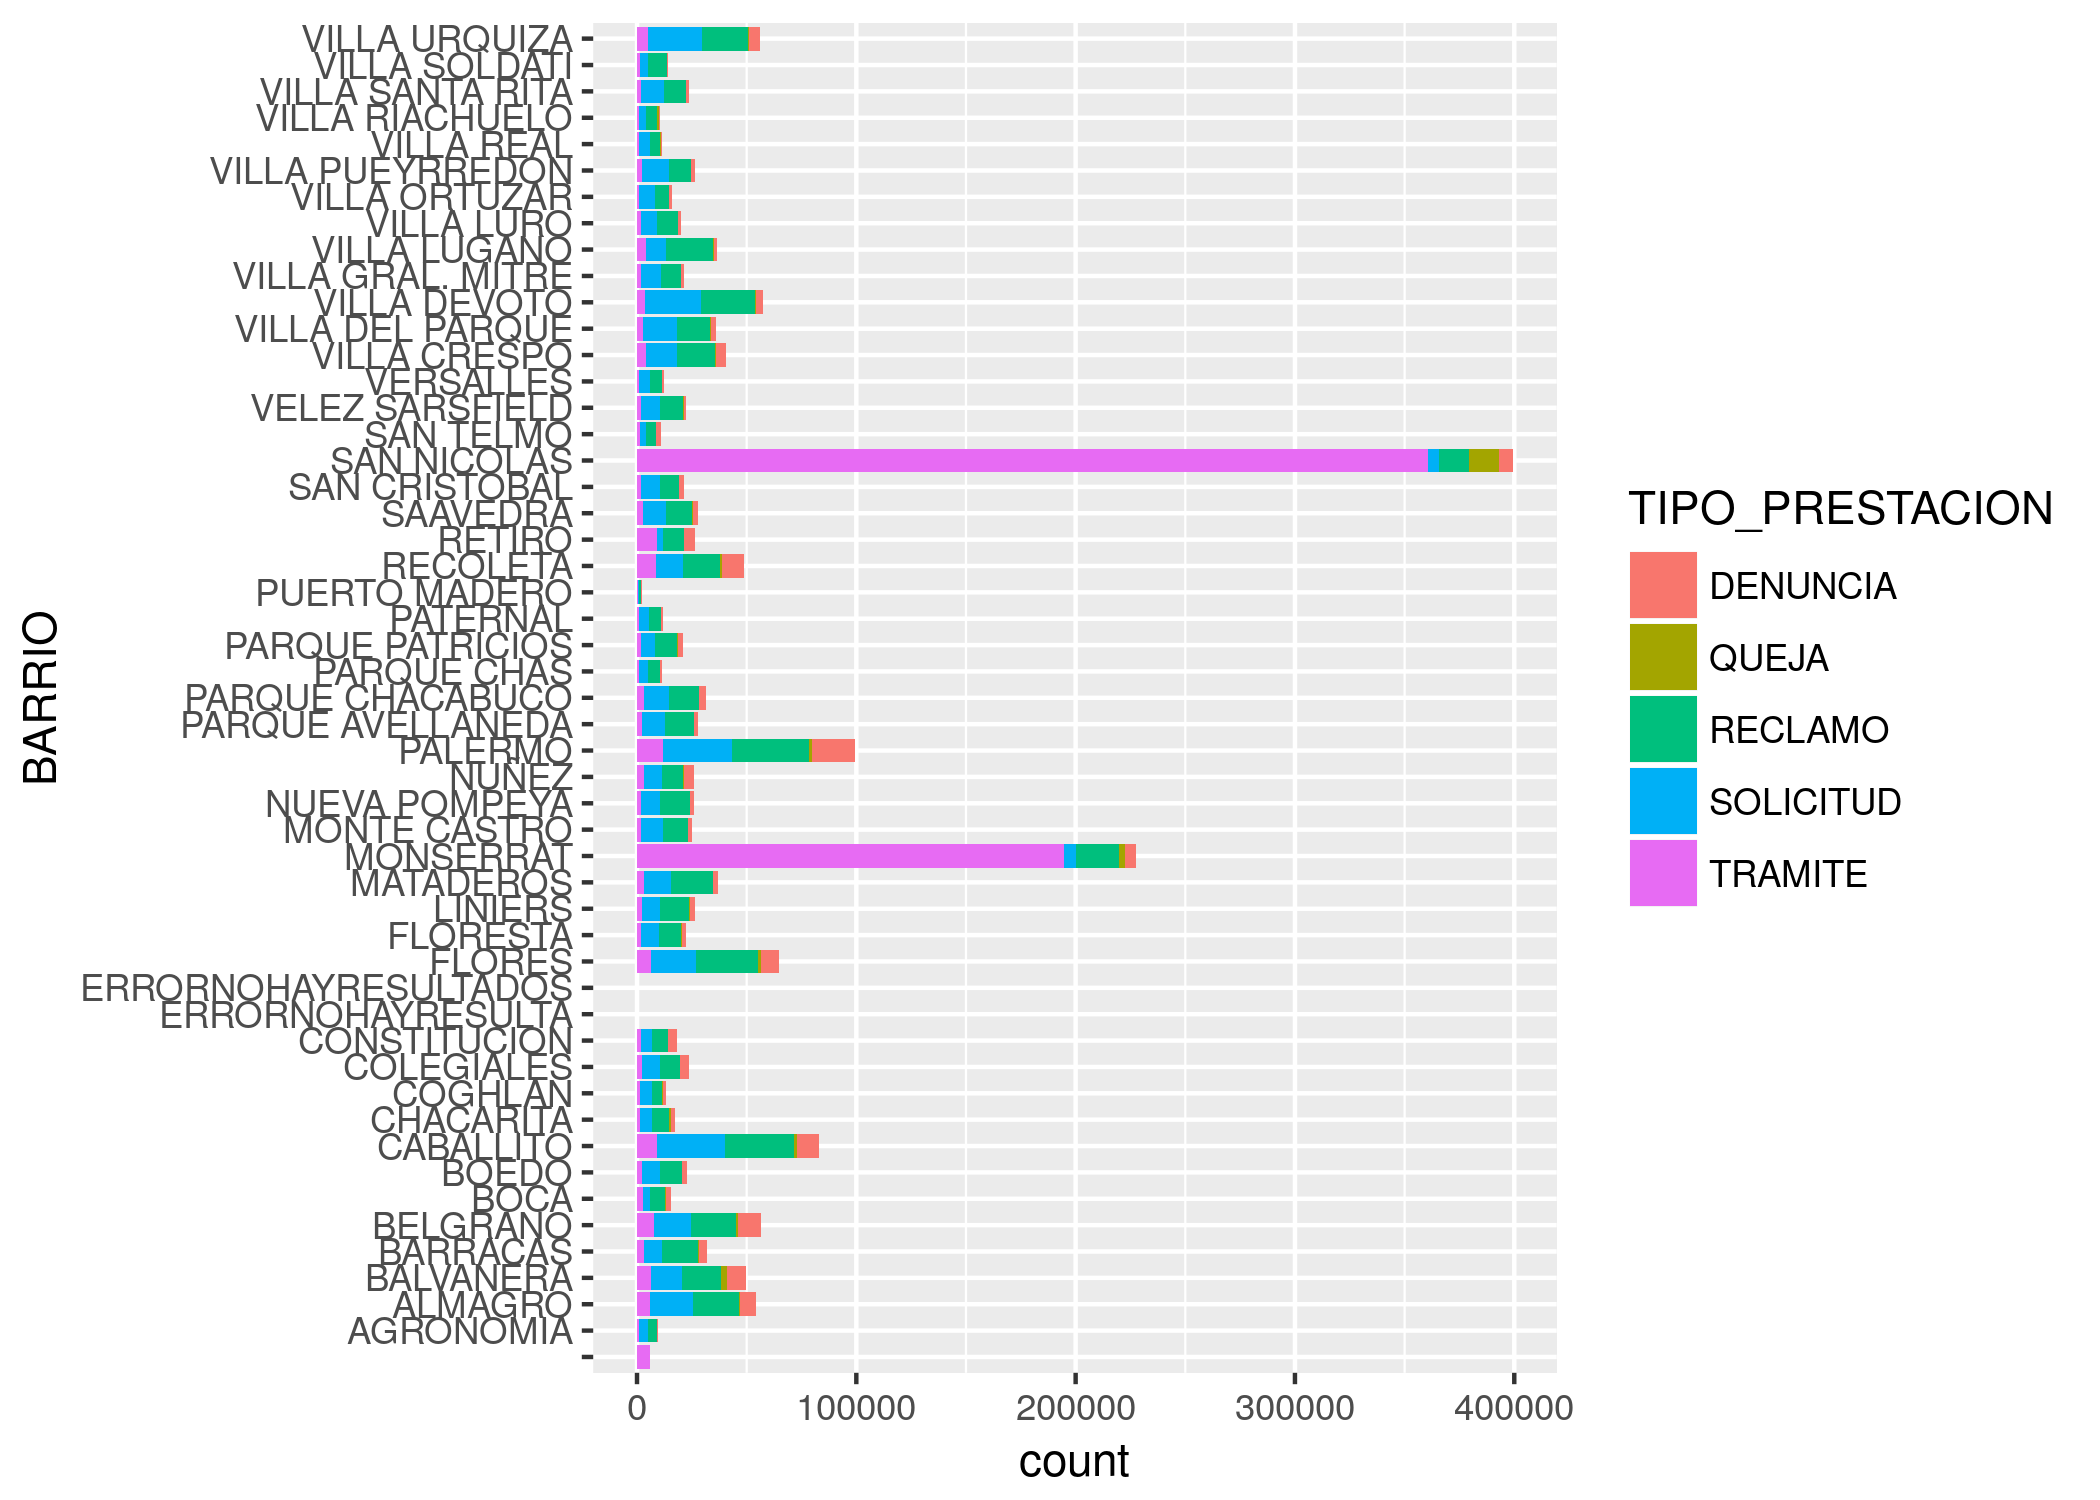
\includegraphics{ciencia_de_datos_para_gente_sociable_files/figure-latex/unnamed-chunk-107-1.pdf}

Aparecen las diferencias. Los reclamos tienen una dispersión mínima, con
casi todas las observaciones apiladas en torno a unos 1000 contactos
mensuales; siempre son bajas. La cantidad mensual de denuncias, reclamos
y solicitudes muestra una dispersión mayor, pero aún así tendencia a
rondar un valor típico. Los trámites son el extremo opuesto a las
qeujas, ya que muestran una gran dispersión, pudiendo tomar cualquier
valor de menos de 10.000 a más de 40.000 registros de forma bastante
pareja.

\section{Preparando una visualización para
compartir}\label{preparando-una-visualizacion-para-compartir}

Lo último que nos queda por decir en este capítulo es que los gráficos
que hemos producido hasta aquí están pensandos para nuestro propio
consumo. Son parte, y parte dundamental, de lo que llamamos análisis
exploratorio de datos. En el contexto de la exploración, lo importante
es trabajar en forma rápida, probando una u otra técnica de
visuzalización y refinando nuestros resultados hasta hallar patrones
interesantes, o sacarnos dudas acerca de los datos. No necesitamos
ponerle título a las visualizaciones, porque ya sabemos de que tratan
(¡acabamos de escribirlas!). No nos preocupa que los nombres de los ejes
indiquen en forma clara la variable representan, porque ya lo sabemos de
antemano.

Pero cuando queremos guardar un gráfico para compartir con otros, sea
publicándola en un paper, o enviándola por mail a un amigo, necesitamos
tener más cuidado. Hemos pasado del ámbito de la exploración al de la
comunicación. Ahora si debe preocuparnos la claridad, porque no sabemos
el grado de familiaridad que tiene con los datos la eventual audiencia.

Si bien la comunicación clara es un arte cuyas reglas dependen del
contexto, y además cada quien tiene su estilo, podemos decretar al menos
tres elementos que no deberían faltar en un gráfico destinado a
comunicar algo a los demás:

\begin{itemize}
\tightlist
\item
  Un título descriptivo, pero breve
\item
  Etiquetas claras (no ambiguas) en los ejes
\item
  Nombres descriptivos en las leyendas
\end{itemize}

y ya que estamos, dos opcionales:

\begin{itemize}
\tightlist
\item
  Un subtítulo donde poner detalles importantes que no entran en un
  título breve
\item
  Una nota al pie con infromación adicional: fuente de los datos, cita
  académica, advertencias, etc.
\end{itemize}

Con \texttt{ggplot()} podemos encargarnos de todo dentro de una sola
función, \texttt{labs()} (por \emph{labels}, etiquetas)

Tomemos un gráfico de los que hicimos antes para pulirlo un poco y que
sirva de ejemplo. El original:

\begin{Shaded}
\begin{Highlighting}[]
\KeywordTok{ggplot}\NormalTok{(atencion_ciudadano) }\OperatorTok{+}
\StringTok{    }\KeywordTok{geom_bar}\NormalTok{(}\KeywordTok{aes}\NormalTok{(}\DataTypeTok{x =}\NormalTok{ BARRIO, }\DataTypeTok{weight =}\NormalTok{ total, }\DataTypeTok{fill =}\NormalTok{ TIPO_PRESTACION)) }\OperatorTok{+}
\StringTok{    }\KeywordTok{coord_flip}\NormalTok{()}
\end{Highlighting}
\end{Shaded}

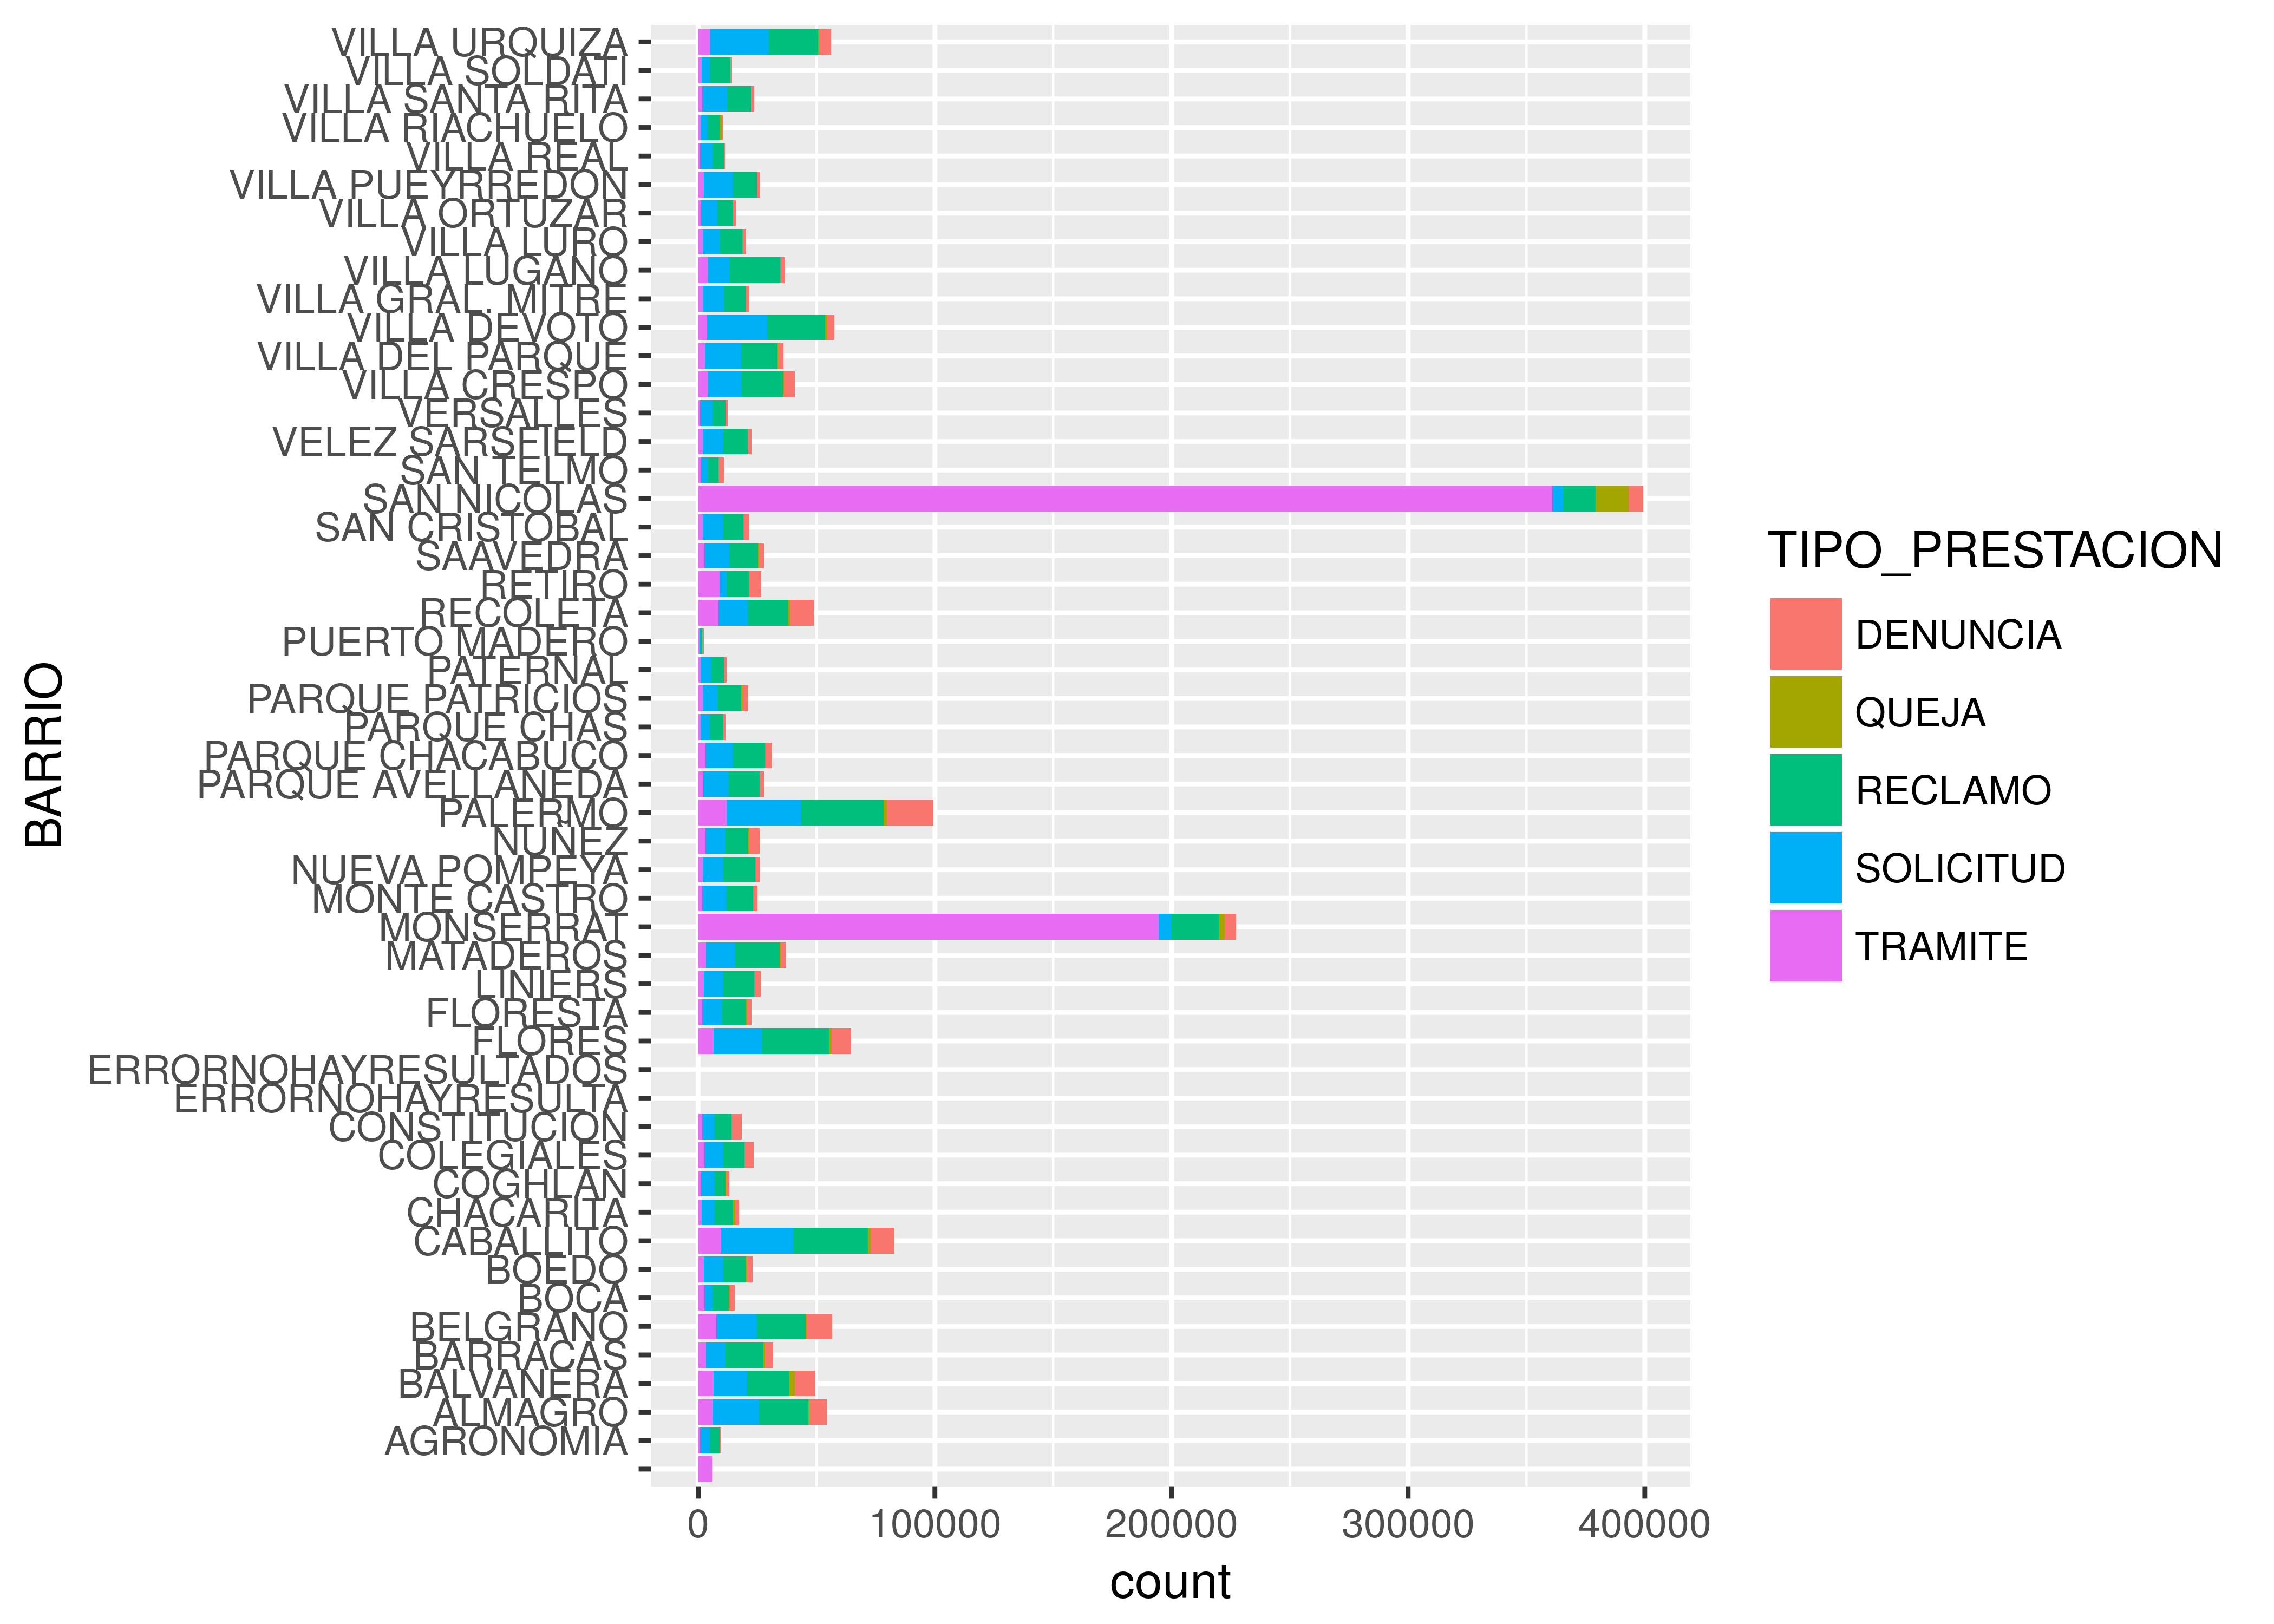
\includegraphics{ciencia_de_datos_para_gente_sociable_files/figure-latex/unnamed-chunk-108-1.pdf}

versus la versión pulida usando \texttt{labs()}:

\begin{Shaded}
\begin{Highlighting}[]
\KeywordTok{ggplot}\NormalTok{(atencion_ciudadano) }\OperatorTok{+}
\StringTok{    }\KeywordTok{geom_bar}\NormalTok{(}\KeywordTok{aes}\NormalTok{(}\DataTypeTok{x =}\NormalTok{ BARRIO, }\DataTypeTok{weight =}\NormalTok{ total, }\DataTypeTok{fill =}\NormalTok{ TIPO_PRESTACION)) }\OperatorTok{+}
\StringTok{    }\KeywordTok{coord_flip}\NormalTok{() }\OperatorTok{+}
\StringTok{    }\KeywordTok{labs}\NormalTok{(}\DataTypeTok{title =} \StringTok{"Contactos realizados al Sistema Único de Atención Ciudadana"}\NormalTok{,}
         \DataTypeTok{subtitle =} \StringTok{"Ciudad Autónoma de Buenos Aires, 2013 - 2015"}\NormalTok{,}
         \DataTypeTok{caption =} \StringTok{"Fuente: portal de datos abiertos de la Ciudad - http://data.buenosaires.gob.ar"}\NormalTok{,}
         \DataTypeTok{x =} \StringTok{"barrio"}\NormalTok{,}
         \DataTypeTok{y =} \StringTok{"cantidad"}\NormalTok{,}
         \DataTypeTok{fill =} \StringTok{"Motivo del contacto"}\NormalTok{)}
\end{Highlighting}
\end{Shaded}

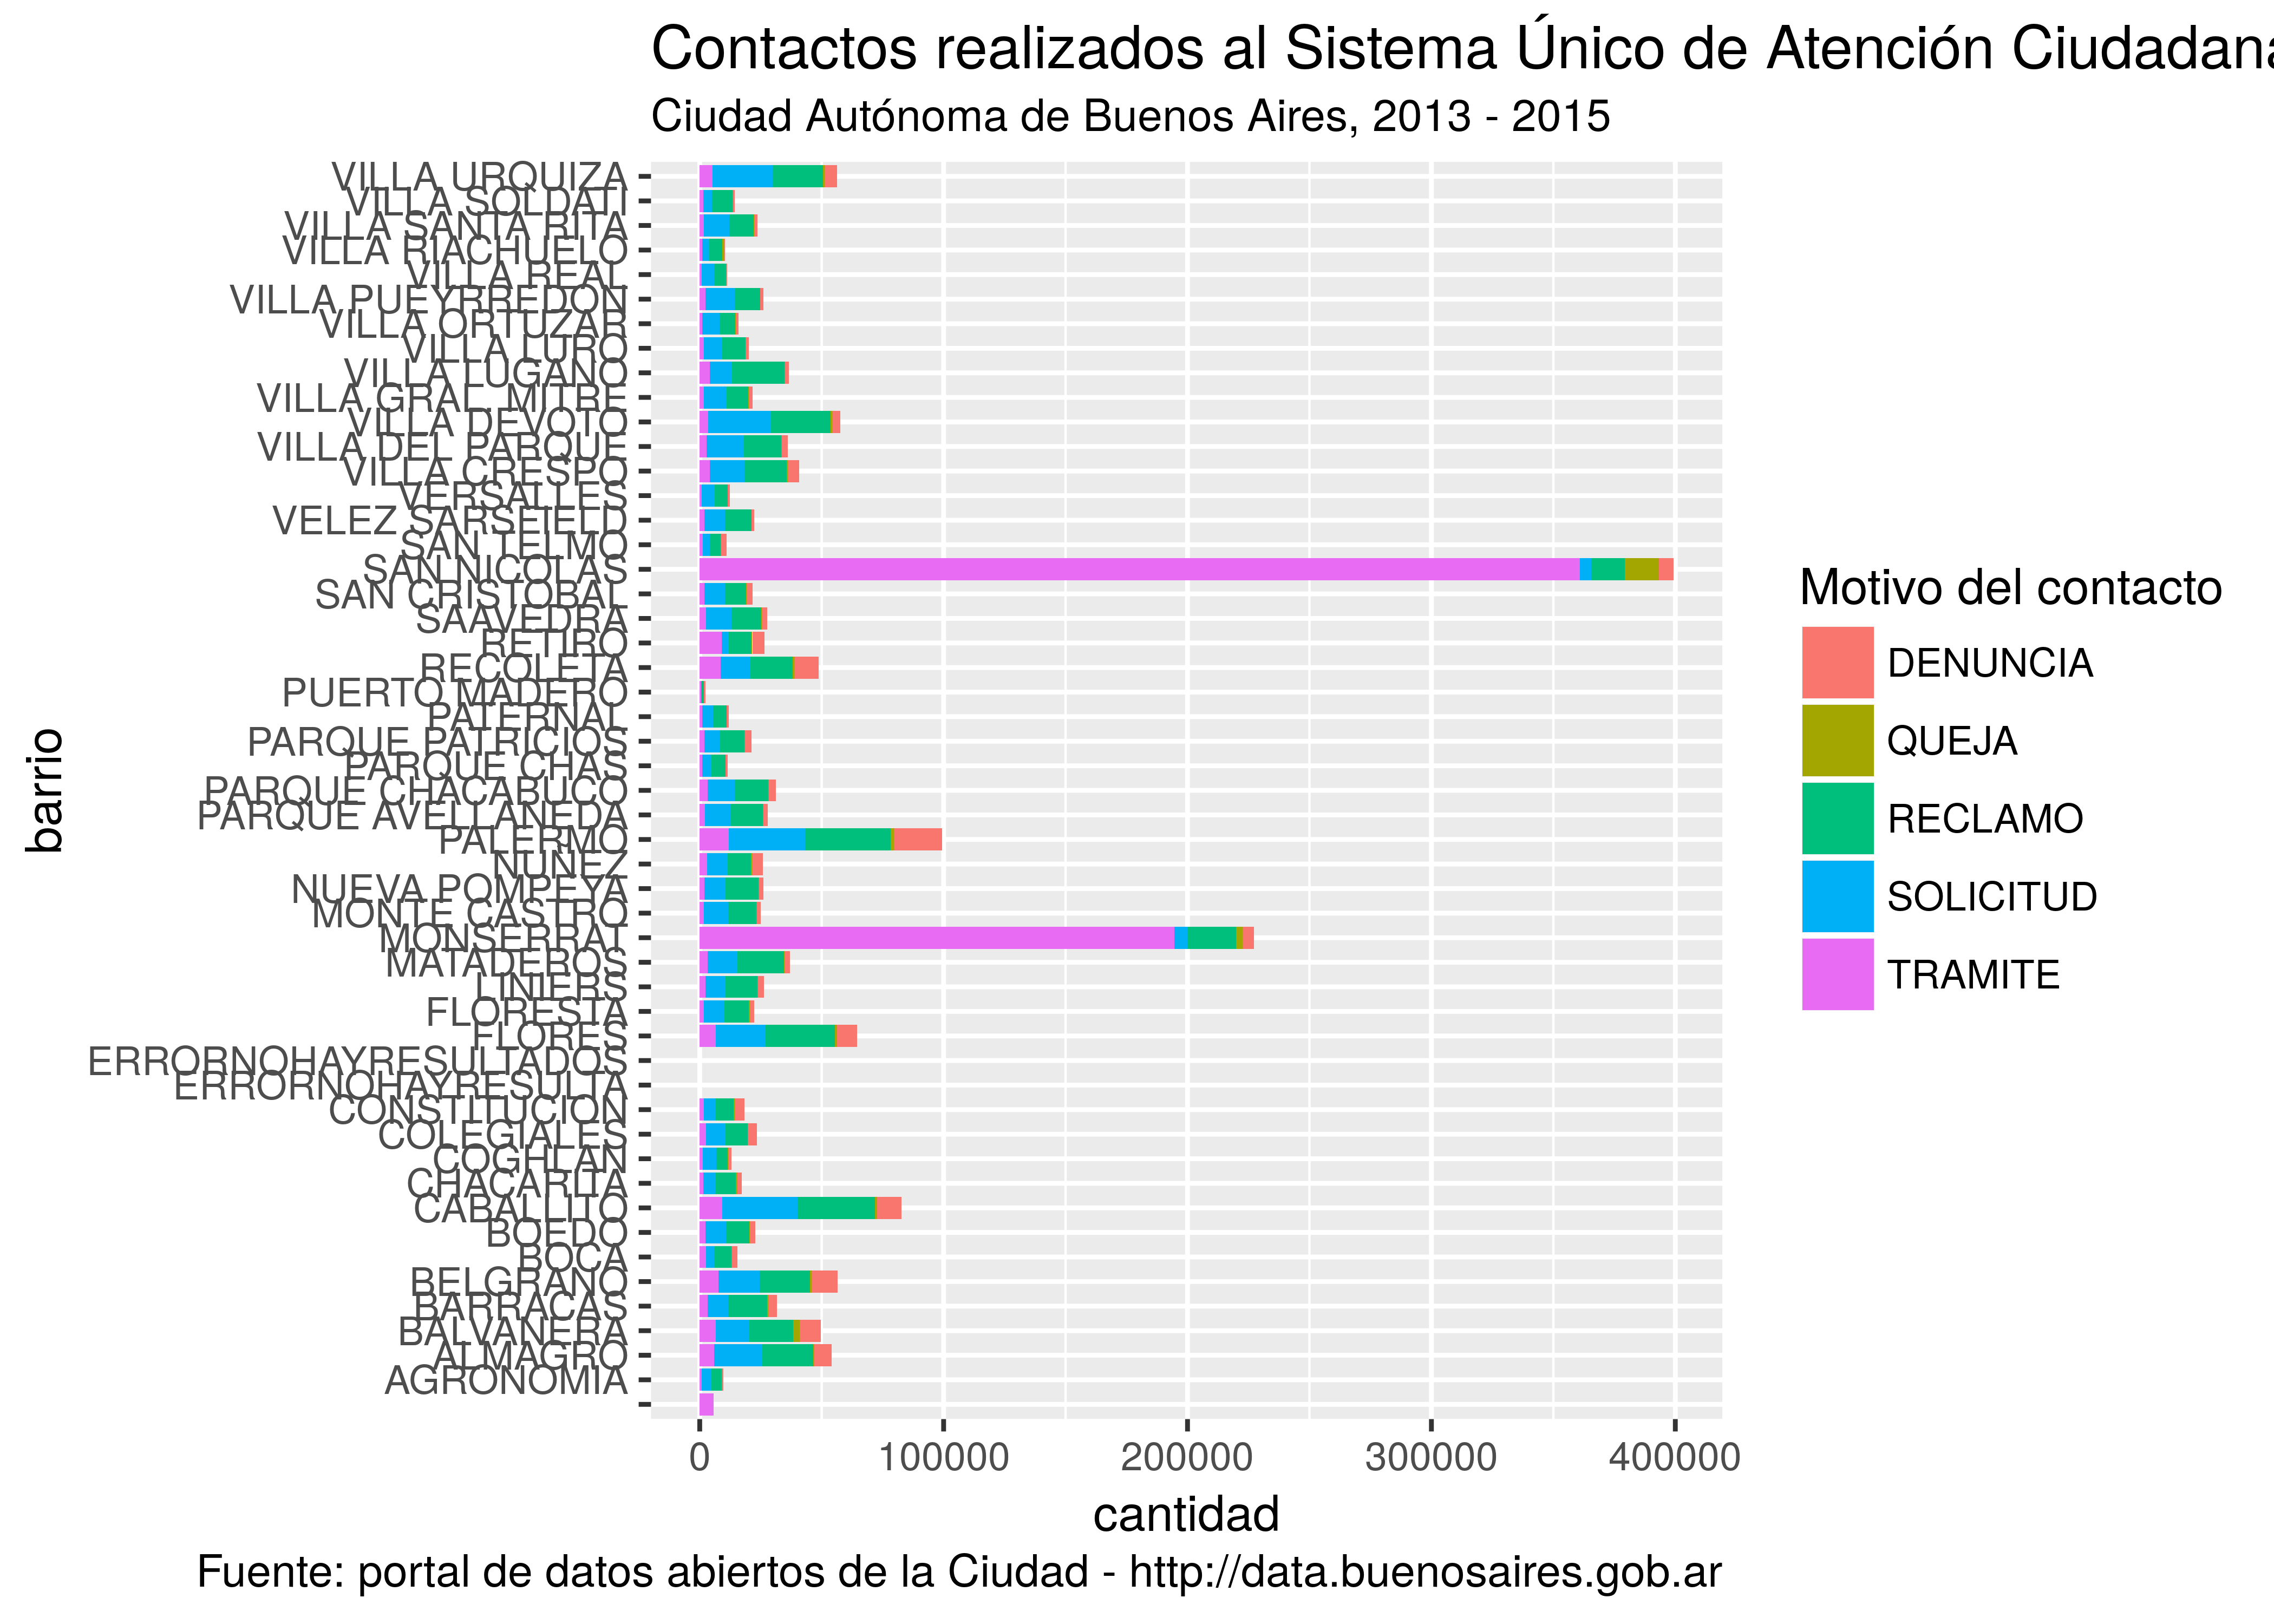
\includegraphics{ciencia_de_datos_para_gente_sociable_files/figure-latex/unnamed-chunk-109-1.pdf}

Ahora si, a compartir.

\section{Otras visualizaciones}\label{otras-visualizaciones}

Por supuesto, las opciones que hemos repasado son apenas una fracción de
la enorme variedad de técnicas de visualización que existen. Para
empezar, nos falta hablar de los mapas, una categoría tan importante que
tiene un capítulo completo dedicado más adelante.

Y aún quedan tantas por discutir, que sería imposible hacerles justicia
en un libro introductorio. Con nombres tan variopintos como \emph{waffle
charts}, \emph{violin plots}, o \emph{tree maps}, existen quizás un
centenar o más de métodos bien documentados para explorar información en
forma visual.

El sitio web Data Viz Project (www.datavizproject.com) es un recurso
excelente para investigar opciones. Contiene un compendio visual e
interactivo de técnicas de visualización con sus nombres, descripción y
ejemplos notables. También explica a que familia corresponde cada una, y
para qué suelen usarse (mostrar relaciones, distribuciones, cambio a
través del tiempo, etc).

\begin{figure}
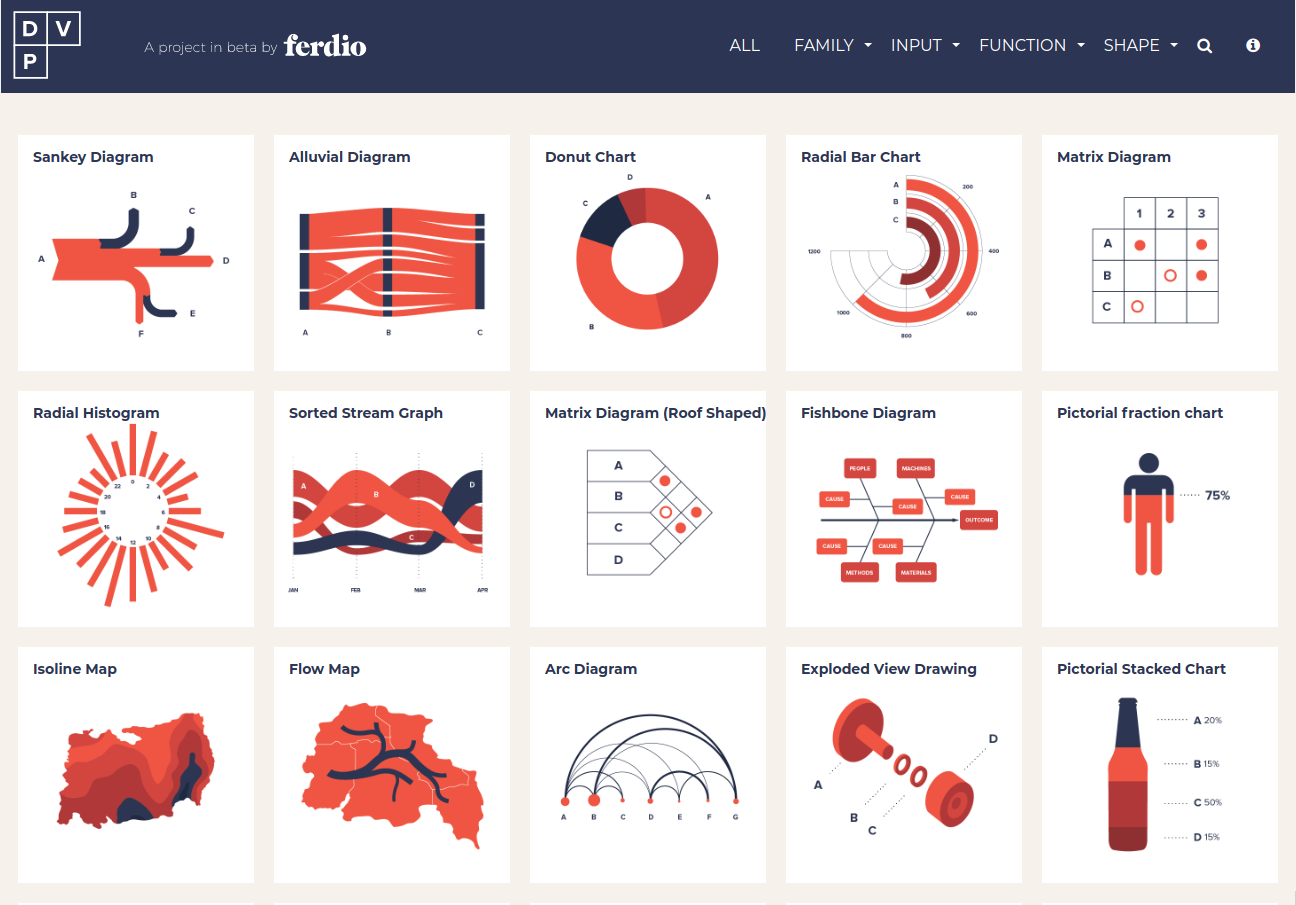
\includegraphics[width=8.64in]{imagenes/data_viz_project} \caption{Data Viz Project - www.datavizproject.com}\label{fig:unnamed-chunk-110}
\end{figure}

Y lo más interesante de todo: con \texttt{ggplot()} podemos realizar
casi todas las visualizaciones presentadas en el sitio, por compejas que
parezcan. Como en tantas otras cosas, Google será el aliado del curioso
autodidacta. Basta con buscar el nombre de la visualización que nos
llame la atencion (por ejemplo, ``ggplot sankey diagram'') para
encontrar ejemplos para copiar e intentar por nuestra cuenta. Con un
poco de suerte, en ocasiones encontraremos un paquete de R que extiende
ggplot para realizar de forma fácil la visualización que nos interesa.

\chapter{Modelado estadístico}\label{modelado-estadistico}

Llegamos a un tema de gran interés para quienes realizan investigaciones
formales. La posición central que tiene el modelado en la investigación
científica se debe a que cuantifica relaciones: permite pasar de decir
``La luz solar abundante mejora el crecimiento de las plantas'' a ``por
cada hora adicional de exposición mensual a la luz solar, los cultivos
aumentaron su rinde en un 1\%''. La cuantificación permite realizar
comparaciones, algo clave para entender un fenómeno estudiado: antes y
después, con o sin tratamiento, en un lugar o en otro.

Este capítulo le debe mucho a \emph{ModernDive: An Introduction to
Statistical and Data Sciences via R} por Chester Ismay y Albert Y. Kim,
disponible en forma gratuita \url{http://http://moderndive.com/}.
ModernDive es un recurso muy recomendable para quienes quieran continuar
profundizando su conocimiento más allá de los temas que veremos a
continuación.

En términos matemáticos, se habla de ``modelar'' debido a que estamos
creando un modelo, una reconstrucción simplificada (¡simplificada en
extremo!) de cómo funciona un proceso observado en el mundo real. En un
modelo de datos, siempre tenemos al menos

\begin{itemize}
\tightlist
\item
  Una variable resultante, siempre una sola, también llamada variable
  ``dependiente'',
\item
  Una o más variables predictoras, también llamadas ``explicativas''
\end{itemize}

El modelado de datos puede ser utilizado para dos propósitos:

\begin{enumerate}
\def\labelenumi{\arabic{enumi}.}
\item
  \textbf{Predecir} el valor de una variable resultante en base a
  valores conocidos de las variables predictoras. Aquí no interesa tanto
  entender cómo es que las variables interactúan entre sí, o por qué lo
  hacen. Mientras las predicciones sean acertadas, o se acerquen lo
  suficiente, el modelo cumple su cometido. Los modelos predictivos se
  emplean en una enorme variedad de aplicaciones: inversión en bolsa,
  prevención de fraude, publicidad online, fijación de primas en seguros
  de riesgo, etc.
\item
  \textbf{Explicar} la relación entre una variable dependiente y todas
  las demás (las explicativas), buscando determinar si la relación es
  significativa. Los modelos explicativos son los que se favorecen en
  investigación académica, ya que ayudan a entender el fenómeno
  modelado.
\end{enumerate}

Existen muchísimas técnicas para modelar datos, algunas de ellas simples
como la regresión lineal, y otras mucho más complejas, como las redes
neuronales. Por supuesto, vamos a practicar con las primeras.

La humilde regresión lineal, fácil de explicar y muy fácil de resolver
con la ayuda de una computadora, es el caballito de batalla del modelado
estadístico. A pesar de que no es adecuada para ciertos tipo de datos, y
de que existen métodos más modernos que explotan con intensidad el
potencial de las computadoras, la regresión lineal sigue siendo la
herramienta más común. Un poco por costumbre, y otro porque es el método
más fácil de interpretar, lo que favorece entender y comunicar sus
resultados.

\section{Regresión lineal simple}\label{regresion-lineal-simple}

La encarnación más sencilla de la regresión lineal es la simple o
univariada. Tenemos nuestra variable \(y\), numérica, y una sola
variable predictora \(x\), que puede ser numérica o categórica.

Para poner en práctica los conceptos repasados en este capítulo, vamos a
tomarnos un recreo de los datos de Buenos Aires, haciendo un \emph{zoom
out} hacia las escalas de país, continente y el planeta entero. Contamos
con un dataset muy prolijo e interesante recopilado por Gapminder
(www.gapminder.org), una organización que busca ``hacer comprensible al
mundo en base a estadísticas confiables''.

Descarguemos el dataset y echémosle un vistazo como ya sabemos hacer:

\begin{Shaded}
\begin{Highlighting}[]
\NormalTok{data_mundial <-}\StringTok{ }\KeywordTok{read.csv}\NormalTok{(}\StringTok{"https://bitsandbricks.github.io/data/gapminder.csv"}\NormalTok{)}

\KeywordTok{summary}\NormalTok{(data_mundial)}
\end{Highlighting}
\end{Shaded}

\begin{verbatim}
##           pais         continente       año          expVida     
##  Afghanistan:  12   Africa  :624   Min.   :1952   Min.   :23.60  
##  Albania    :  12   Americas:300   1st Qu.:1966   1st Qu.:48.20  
##  Algeria    :  12   Asia    :396   Median :1980   Median :60.71  
##  Angola     :  12   Europe  :360   Mean   :1980   Mean   :59.47  
##  Argentina  :  12   Oceania : 24   3rd Qu.:1993   3rd Qu.:70.85  
##  Australia  :  12                  Max.   :2007   Max.   :82.60  
##  (Other)    :1632                                                
##       pobl                PBI_PC        
##  Min.   :     60011   Min.   :   241.2  
##  1st Qu.:   2793664   1st Qu.:  1202.1  
##  Median :   7023596   Median :  3531.8  
##  Mean   :  29601212   Mean   :  7215.3  
##  3rd Qu.:  19585222   3rd Qu.:  9325.5  
##  Max.   :1318683096   Max.   :113523.1  
## 
\end{verbatim}

Con el poder de \texttt{summary()}, podemos decir unas cuantas cosas
acerca de nuestros dataset. Las observaciones son de un país, su
continente, un año determinado y su expectativa de vida, población
y\ldots{} ¿PBI\_PC?. Esa última es PBI per cápita. Que, según parece,
hay 12 observaciones por país. Que el rango de años es de 1952 a 2007.
Que a lo largo de esos años, la menor expectativa registrada ha sido de
23 años (¡uf!) y la mayor de 82. Que el país menos poblado en el dataset
ha tenido apenas más de 60.000 habitantes, mientras que el más populoso
ha alcanzado los 1300 millones.

\subsection{Regresión con una variable
numérica}\label{regresion-con-una-variable-numerica}

Hagamos nuestra pregunta: ¿Cómo ha se relaciona el paso del tiempo
(variable explicativa) con la expectativa de vida en la Argentina?

Para contestar, primero filtremos los datos que nos interesan:

\begin{Shaded}
\begin{Highlighting}[]
\NormalTok{data_arg <-}\StringTok{ }\NormalTok{data_mundial }\OperatorTok\StringTok{ }
\StringTok{    }\KeywordTok{filter}\NormalTok{(pais }\OperatorTok{==}\StringTok{ "Argentina"}\NormalTok{)}

\NormalTok{data_arg}
\end{Highlighting}
\end{Shaded}

\begin{verbatim}
##         pais continente  año expVida     pobl    PBI_PC
## 1  Argentina   Americas 1952  62.485 17876956  5911.315
## 2  Argentina   Americas 1957  64.399 19610538  6856.856
## 3  Argentina   Americas 1962  65.142 21283783  7133.166
## 4  Argentina   Americas 1967  65.634 22934225  8052.953
## 5  Argentina   Americas 1972  67.065 24779799  9443.039
## 6  Argentina   Americas 1977  68.481 26983828 10079.027
## 7  Argentina   Americas 1982  69.942 29341374  8997.897
## 8  Argentina   Americas 1987  70.774 31620918  9139.671
## 9  Argentina   Americas 1992  71.868 33958947  9308.419
## 10 Argentina   Americas 1997  73.275 36203463 10967.282
## 11 Argentina   Americas 2002  74.340 38331121  8797.641
## 12 Argentina   Americas 2007  75.320 40301927 12779.380
\end{verbatim}

Como dijimos en el capítulo de visualización, los scatterplots son
útiles para mostrar la relación entre dos variables. Usemos uno para
visualizar la relación entre año y expectativa de vida en Argentina,
para intentar anticipar los resultados de la regresión lineal.

\begin{Shaded}
\begin{Highlighting}[]
\KeywordTok{ggplot}\NormalTok{(}\DataTypeTok{data =}\NormalTok{ data_arg) }\OperatorTok{+}\StringTok{ }
\StringTok{    }\KeywordTok{geom_point}\NormalTok{(}\KeywordTok{aes}\NormalTok{(}\DataTypeTok{x =}\NormalTok{ año, }\DataTypeTok{y =}\NormalTok{ expVida)) }\OperatorTok{+}
\StringTok{    }\KeywordTok{labs}\NormalTok{(}\DataTypeTok{title =} \StringTok{"Correlación entre tiempo y expectativa de vida"}\NormalTok{,}
         \DataTypeTok{subtitle =} \StringTok{"Argentina"}\NormalTok{,}
         \DataTypeTok{y =} \StringTok{"expectativa de vida"}\NormalTok{)}
\end{Highlighting}
\end{Shaded}


\includegraphics{ciencia_de_datos_para_gente_sociable_files/figure-latex/unnamed-chunk-113-1.pdf}

Bien, no necesitamos recurrir a la matemática para saber que tiempo y
expectativa de vida están correlacionadas en forma positiva. Esto es, el
incremento de una unidad de tiempo en general (o siempre, en este caso)
resulta en el incremento de la expectativa de vida. Una correlación
\emph{negativa} sería lo opuesto: que el incremento de la variable
explicativa estuviera asociado a un decremento de la variable explicada.
Además del \emph{signo} de una correlación, otra medida importante es su
intensidad. La intensidad de una correlación va de -1 (correlación
negativa total) a 1 (correlación positiva total). Una correlación de
cero significa que las dos variables son por completo independientes. En
en ese caso, saber cuánto vale una no nos ayuda a estimar el valor de la
otra.

Obtener la correlación entre dos variables es fácil. La función
\texttt{cor()} toma dos vectores dos secuencias de valores, y los
compara para determinar su grado de correlación. Recurriendo al truco
que ya usamos alguna vez, usamos el formato ``dataframe\$columna'' para
extraer las columnas de nuestro dataframe que necesitamos:

\begin{Shaded}
\begin{Highlighting}[]
\KeywordTok{cor}\NormalTok{(data_arg}\OperatorTok{$}\NormalTok{año, data_arg}\OperatorTok{$}\NormalTok{expVida)}
\end{Highlighting}
\end{Shaded}

\begin{verbatim}
## [1] 0.9977816
\end{verbatim}

¿A partir de qué valor consideramos que existe una correlación
apreciable? La verdad es que no hay una regla a seguir, pero inventemos
una. Si el valor absoluto de la correlación es..

\begin{verbatim}
- de 0,7 a 1: de fuerte a total
- de 0,5 a 0,7: de moderada a fuerte
- de 0,3 a 0,7: de débil a moderada
- menor a 0,3: de nula a débil
\end{verbatim}

El valor que obtuvimos se acerca mucho a 1, la correlación casi total.
OK, el paso de los años y la expectativa de vida en la Argentina están
correlacionados de forma intensa, pero aún desconocemos algo quizás más
importante: un valor preciso del ``efecto'' que el paso de cada año
tiene sobre la expectativa de vida. Eso es lo que vamos a determinar con
la regresión lineal. Usamos la palabra ``efecto'' entre comillas para
aclarar una de las limitaciones del modelado estadístico: podemos probar
correlación, pero no causalidad. Es decir, no podemos probar que una
variable causa a la otra; en todo caso, probamos que se mueven juntas y
en base a ello podríamos diseñar un experimento que permita comprobar
causalidad.

Vamos a la regresión lineal entonces, para medir de una buena vez la
correlación entre tiempo y expectativa de vida. Usamos la función
\texttt{lm()} (por ``linear model''), así:

\begin{Shaded}
\begin{Highlighting}[]
\NormalTok{modelo_exp <-}\StringTok{ }\KeywordTok{lm}\NormalTok{(expVida }\OperatorTok{~}\StringTok{ }\NormalTok{año, }\DataTypeTok{data =}\NormalTok{ data_arg)}
\end{Highlighting}
\end{Shaded}

¡Eso es todo! Hemos construido un modelo estadístico; ahora tenemos que
aprender a usarlo. Obsérvese que volvió aparecer el simbolillo que
denota una fórmula, \texttt{\textasciitilde{}}. Usado como primer
argumento de \texttt{lm()}, significa ``\emph{expVida} vs \emph{año}'',
es decir ``estimar el efecto en la variable \emph{expVida} cuando
incrementa el valor de \emph{año}'', usando los datos contenidos en el
dataframe \emph{data\_arg}.

El resultado de \texttt{lm()}, que hemos guardado dentro de la variable
\texttt{modelo\_exp} es un tipo de objecto con el que no hemos trabajado
hasta ahora. No es un dataframe, sino una lista que contiene distintos
atributos del modelo estadístico. No hace falta preocuparnos por eso
ahora.

Retomando nuestra pregunta\ldots{} ¿cuál es el efecto? Nos lo dice el
modelo cuando lo escribimos.

\begin{Shaded}
\begin{Highlighting}[]
\NormalTok{modelo_exp}
\end{Highlighting}
\end{Shaded}

\begin{verbatim}
## 
## Call:
## lm(formula = expVida ~ año, data = data_arg)
## 
## Coefficients:
## (Intercept)          año  
##   -389.6063       0.2317
\end{verbatim}

Ahí está. En nuestro modelo, el \emph{coeficiente} de la variable
``año'' es 0.2317. Significado: incrementando en una unidad la variable
año, la variable expectativa de vida se incrementa en 0.2317. Dicho de
otra manera, por cada año que pasa la expectativa de vida en la
Argentina aumenta casi 3 meses.

El otro coeficiente que aparece, ``(Intercept)'' es la intersección. En
términos de interpretado del modelo, la intersección rara vez tiene
utilidad. Para lo que sí sirve es para trazar la línea que permite
``predecir'' valores para años en los que no tenemos observaciones.
Recordemos la fórmula que define una línea recta:

\[ y = a + b \times x \]

A cada punto en \(x\) le corresponde un valor en \(y\) que se obtiene
multiplicando a \(x\) por la \emph{pendiente}, \(b\), y sumando la
intersección, \(a\). Se le llama ``intersección'' u ``ordenada al
origen'' porque es el valor donde la recta intersecta con el eje de las
\texttt{y}: cuando \(x\) vale \(0\), la fórmula nos da \(y = b\).

En una regresión lineal, el ``modelo'' que creamos es precisamente eso:
una línea. Tan simple como eso. Lo que hace a esta linea tan potente, es
que la podemos usar bola de cristal: para saber cuanto valdría la
variable dependiente ante un valor determinado de la variable
predictora, revisamos por donde pasa la línea.

Lo podemos visualizar con ayuda de \texttt{ggplot()}, que por supuesto
incluye una función para trazar líneas. Parámetros necesarios:
\emph{intercept} (intersección) y \emph{slope} (pendiente). Usamos los
respectivos valores que nos indica el modelo, \texttt{-389.6063} y
\texttt{o.2317}.

\begin{Shaded}
\begin{Highlighting}[]
\KeywordTok{ggplot}\NormalTok{(}\DataTypeTok{data =}\NormalTok{ data_arg) }\OperatorTok{+}\StringTok{ }
\StringTok{    }\KeywordTok{geom_point}\NormalTok{(}\KeywordTok{aes}\NormalTok{(}\DataTypeTok{x =}\NormalTok{ año, }\DataTypeTok{y =}\NormalTok{ expVida)) }\OperatorTok{+}
\StringTok{    }\KeywordTok{labs}\NormalTok{(}\DataTypeTok{title =} \StringTok{"Correlación entre tiempo y expectativa de vida"}\NormalTok{,}
         \DataTypeTok{subtitle =} \StringTok{"Argentina"}\NormalTok{,}
         \DataTypeTok{y =} \StringTok{"expectativa de vida"}\NormalTok{,}
         \DataTypeTok{caption =} \StringTok{"con línea de regresión") +}
\StringTok{    geom_abline(aes(intercept = -389.6063, slope = 0.2317), color = "}\NormalTok{blue}\StringTok{")}
\end{Highlighting}
\end{Shaded}

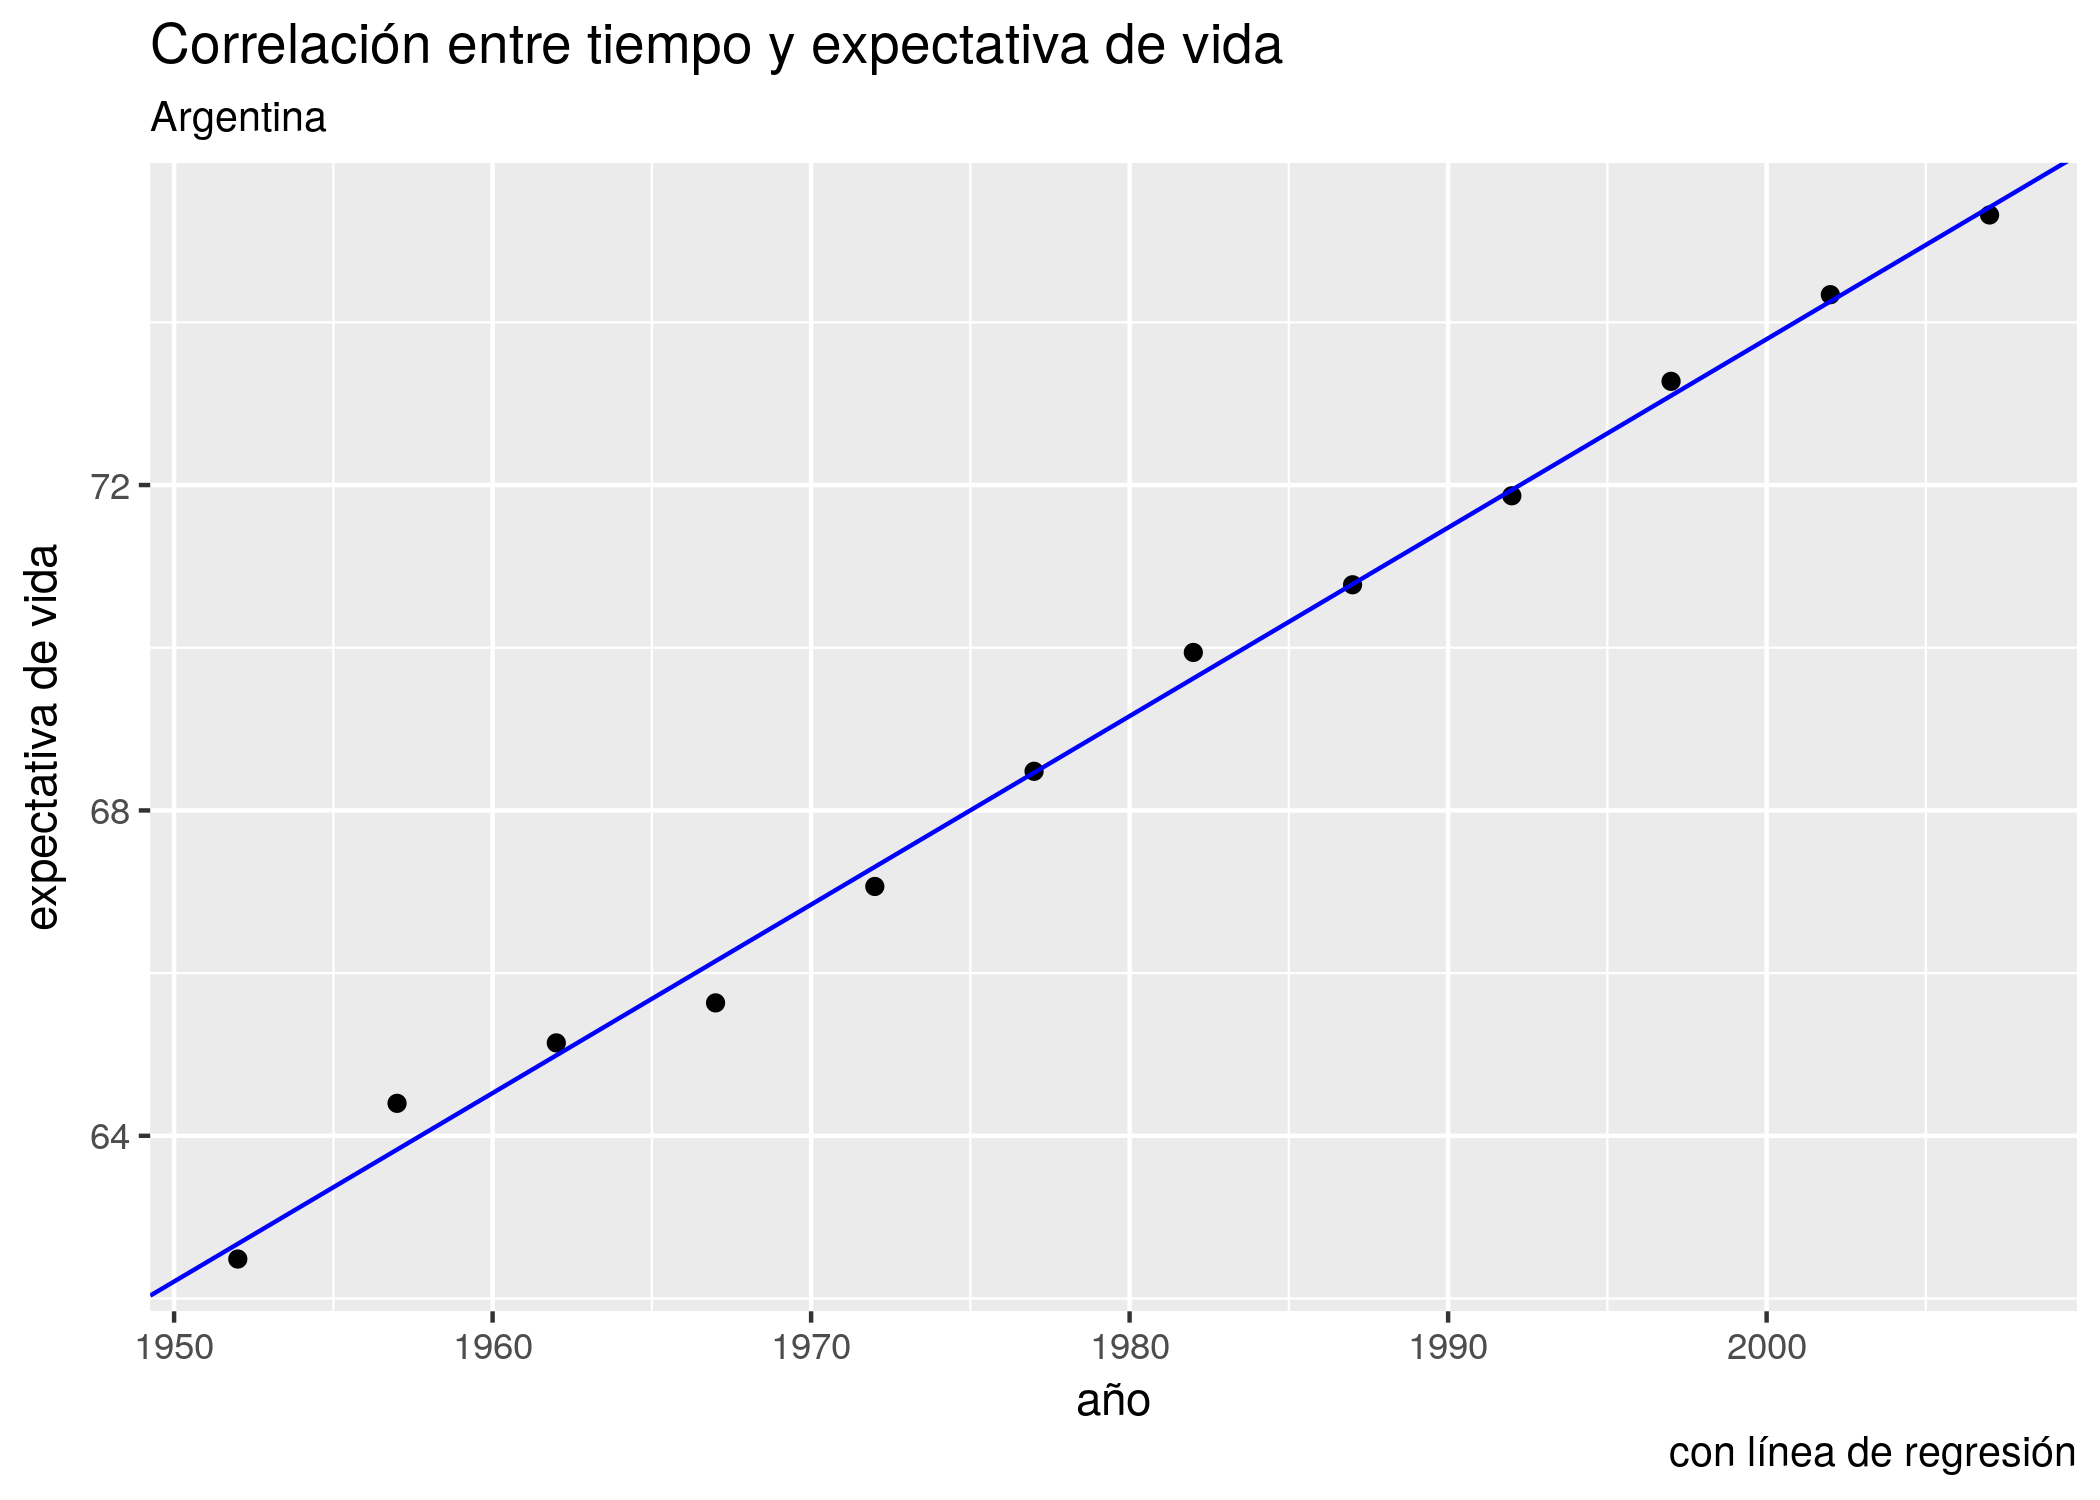
\includegraphics{ciencia_de_datos_para_gente_sociable_files/figure-latex/unnamed-chunk-117-1.pdf}

Aquí no vemos más que los datos que ya teníamos. Pero proyectemos la
línea hacia el futuro. Con \texttt{xlim()} e \texttt{ylim()} podemos
definir a mano los límites de nuestro gráfico, haciéndolo ir más allá
del rango de los datos que tenemos. La línea sigue siendo la misma, sólo
que ahora podemos ver hacia donde va.

\begin{Shaded}
\begin{Highlighting}[]
\KeywordTok{ggplot}\NormalTok{(}\DataTypeTok{data =}\NormalTok{ data_arg) }\OperatorTok{+}\StringTok{ }
\StringTok{    }\KeywordTok{geom_point}\NormalTok{(}\KeywordTok{aes}\NormalTok{(}\DataTypeTok{x =}\NormalTok{ año, }\DataTypeTok{y =}\NormalTok{ expVida)) }\OperatorTok{+}
\StringTok{    }\KeywordTok{labs}\NormalTok{(}\DataTypeTok{title =} \StringTok{"Correlación entre tiempo y expectativa de vida"}\NormalTok{,}
         \DataTypeTok{subtitle =} \StringTok{"Argentina"}\NormalTok{,}
         \DataTypeTok{y =} \StringTok{"expectativa de vida"}\NormalTok{,}
         \DataTypeTok{caption =} \StringTok{"con línea de regresión") +}
\StringTok{    geom_abline(aes(intercept = -389.6063, slope = 0.2317), color = "}\NormalTok{blue}\StringTok{") +}
\StringTok{    xlim(c(1950, 2030)) +}
\StringTok{    ylim(c(60, 85))}
\end{Highlighting}
\end{Shaded}

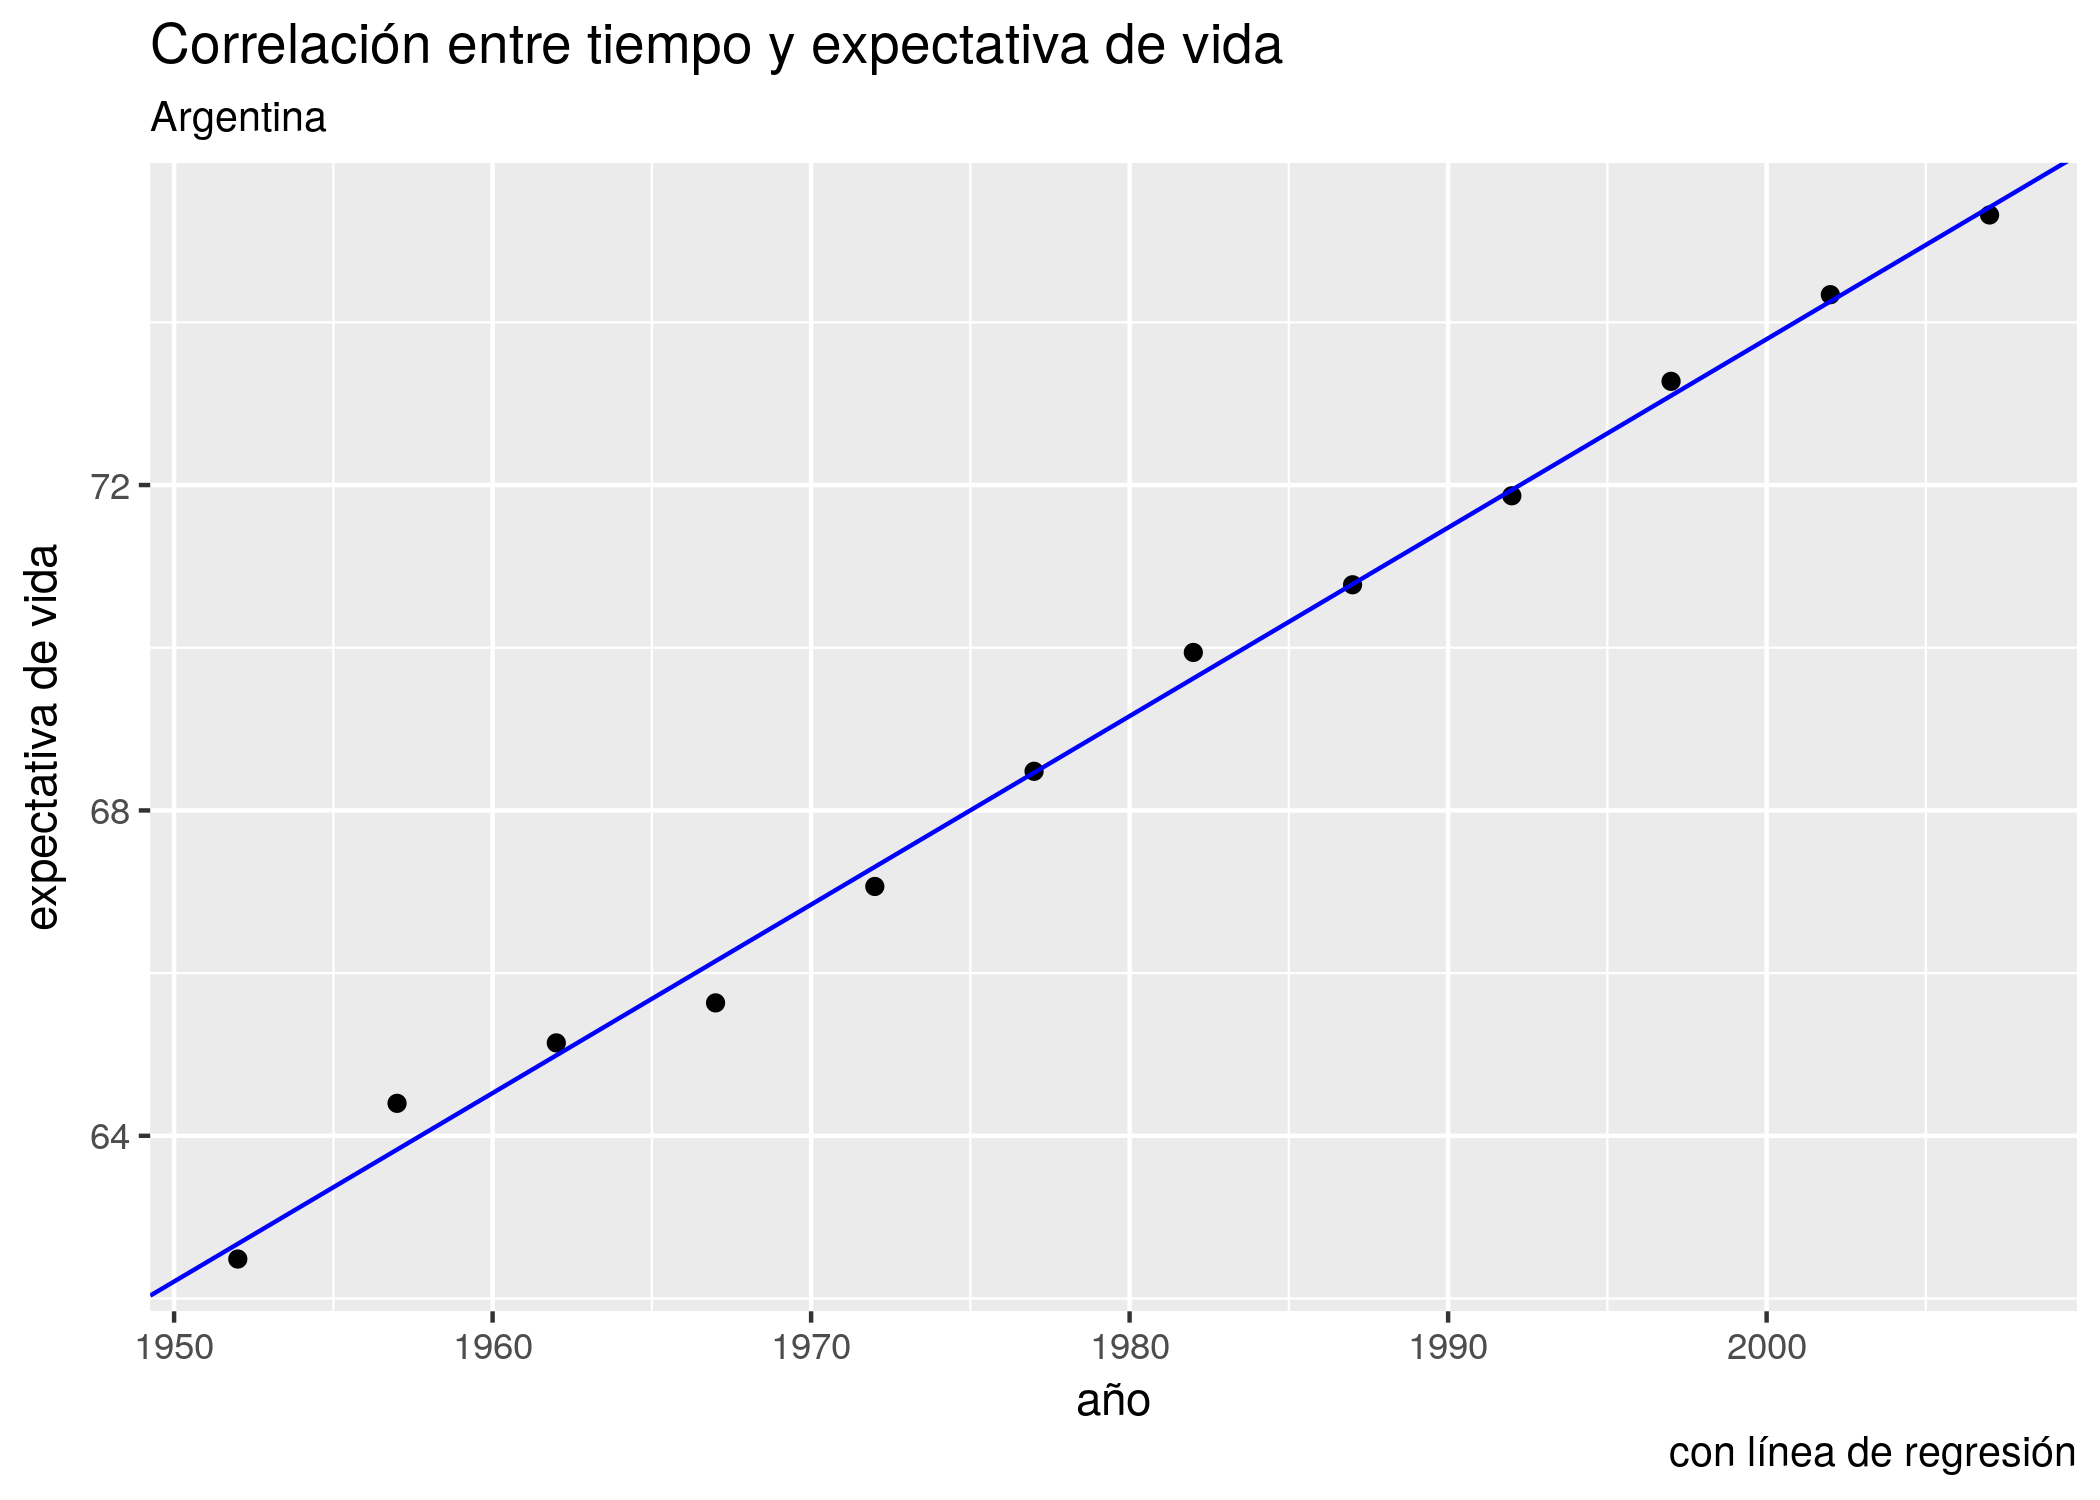
\includegraphics{ciencia_de_datos_para_gente_sociable_files/figure-latex/unnamed-chunk-118-1.pdf}

Ahí está la predicción. Según nuestro modelo, para el año 2030 la
expectativa de vida en la Argentina habrá superado los 80 años.

Es hora de dar una definición oficial para una regresión lineal, y es
esta: es la línea que describe la ecuación:

\[ \hat{y} = b_0 + b_1 \times x \] Obsérvese que se trata de la ecuación
de una recta, \(y = a + b \times x\), con otros nombres. En voz alta, se
leería así ``Cada predicción del valor de y, llamada \(\hat{y}\), se
obtiene multiplicando a la variable predictora \(x\) por su coeficiente
\(b_1\) y sumándole el valor de la intersección \(b_0\)''. En otras
palabras, a cada valor de \(x\) (las observaciones de la variable
explicativa) le corresponde un punto en la recta trazada por el modelo.
La altura sobre la recta de las \(y\) para ese punto es el valor
predicho para la variable dependiente.

Ya que estamos, aprendamos otro truco. \texttt{ggplot()} puede agregar a
nuestros scatterplots una capa con la línea de la regresión lineal, en
forma automática. La función \texttt{geom\_smooth()} se usar para
explicitar patrones en los datos. Tal como otras de la familia ggplot,
espera que se le diga que variables asignar a \texttt{x} e \texttt{y},
más un parámetro \texttt{method} con el método solicitado para trazar
una línea de tendencia. Aquí usamos \texttt{method\ =\ "lm"} por
\emph{linear model}, el modelo lineal.

\begin{Shaded}
\begin{Highlighting}[]
\KeywordTok{ggplot}\NormalTok{(}\DataTypeTok{data =}\NormalTok{ data_arg) }\OperatorTok{+}\StringTok{ }
\StringTok{    }\KeywordTok{geom_point}\NormalTok{(}\KeywordTok{aes}\NormalTok{(}\DataTypeTok{x =}\NormalTok{ año, }\DataTypeTok{y =}\NormalTok{ expVida)) }\OperatorTok{+}
\StringTok{    }\KeywordTok{labs}\NormalTok{(}\DataTypeTok{title =} \StringTok{"Correlación entre tiempo y expectativa de vida"}\NormalTok{,}
         \DataTypeTok{subtitle =} \StringTok{"Argentina"}\NormalTok{,}
         \DataTypeTok{y =} \StringTok{"expectativa de vida"}\NormalTok{,}
         \DataTypeTok{caption =} \StringTok{"con línea de regresión vía geom_smooth()"}\NormalTok{) }\OperatorTok{+}
\StringTok{    }\KeywordTok{geom_smooth}\NormalTok{(}\KeywordTok{aes}\NormalTok{(}\DataTypeTok{x =}\NormalTok{ año, }\DataTypeTok{y =}\NormalTok{ expVida), }\DataTypeTok{method =} \StringTok{"lm"}\NormalTok{)}
\end{Highlighting}
\end{Shaded}

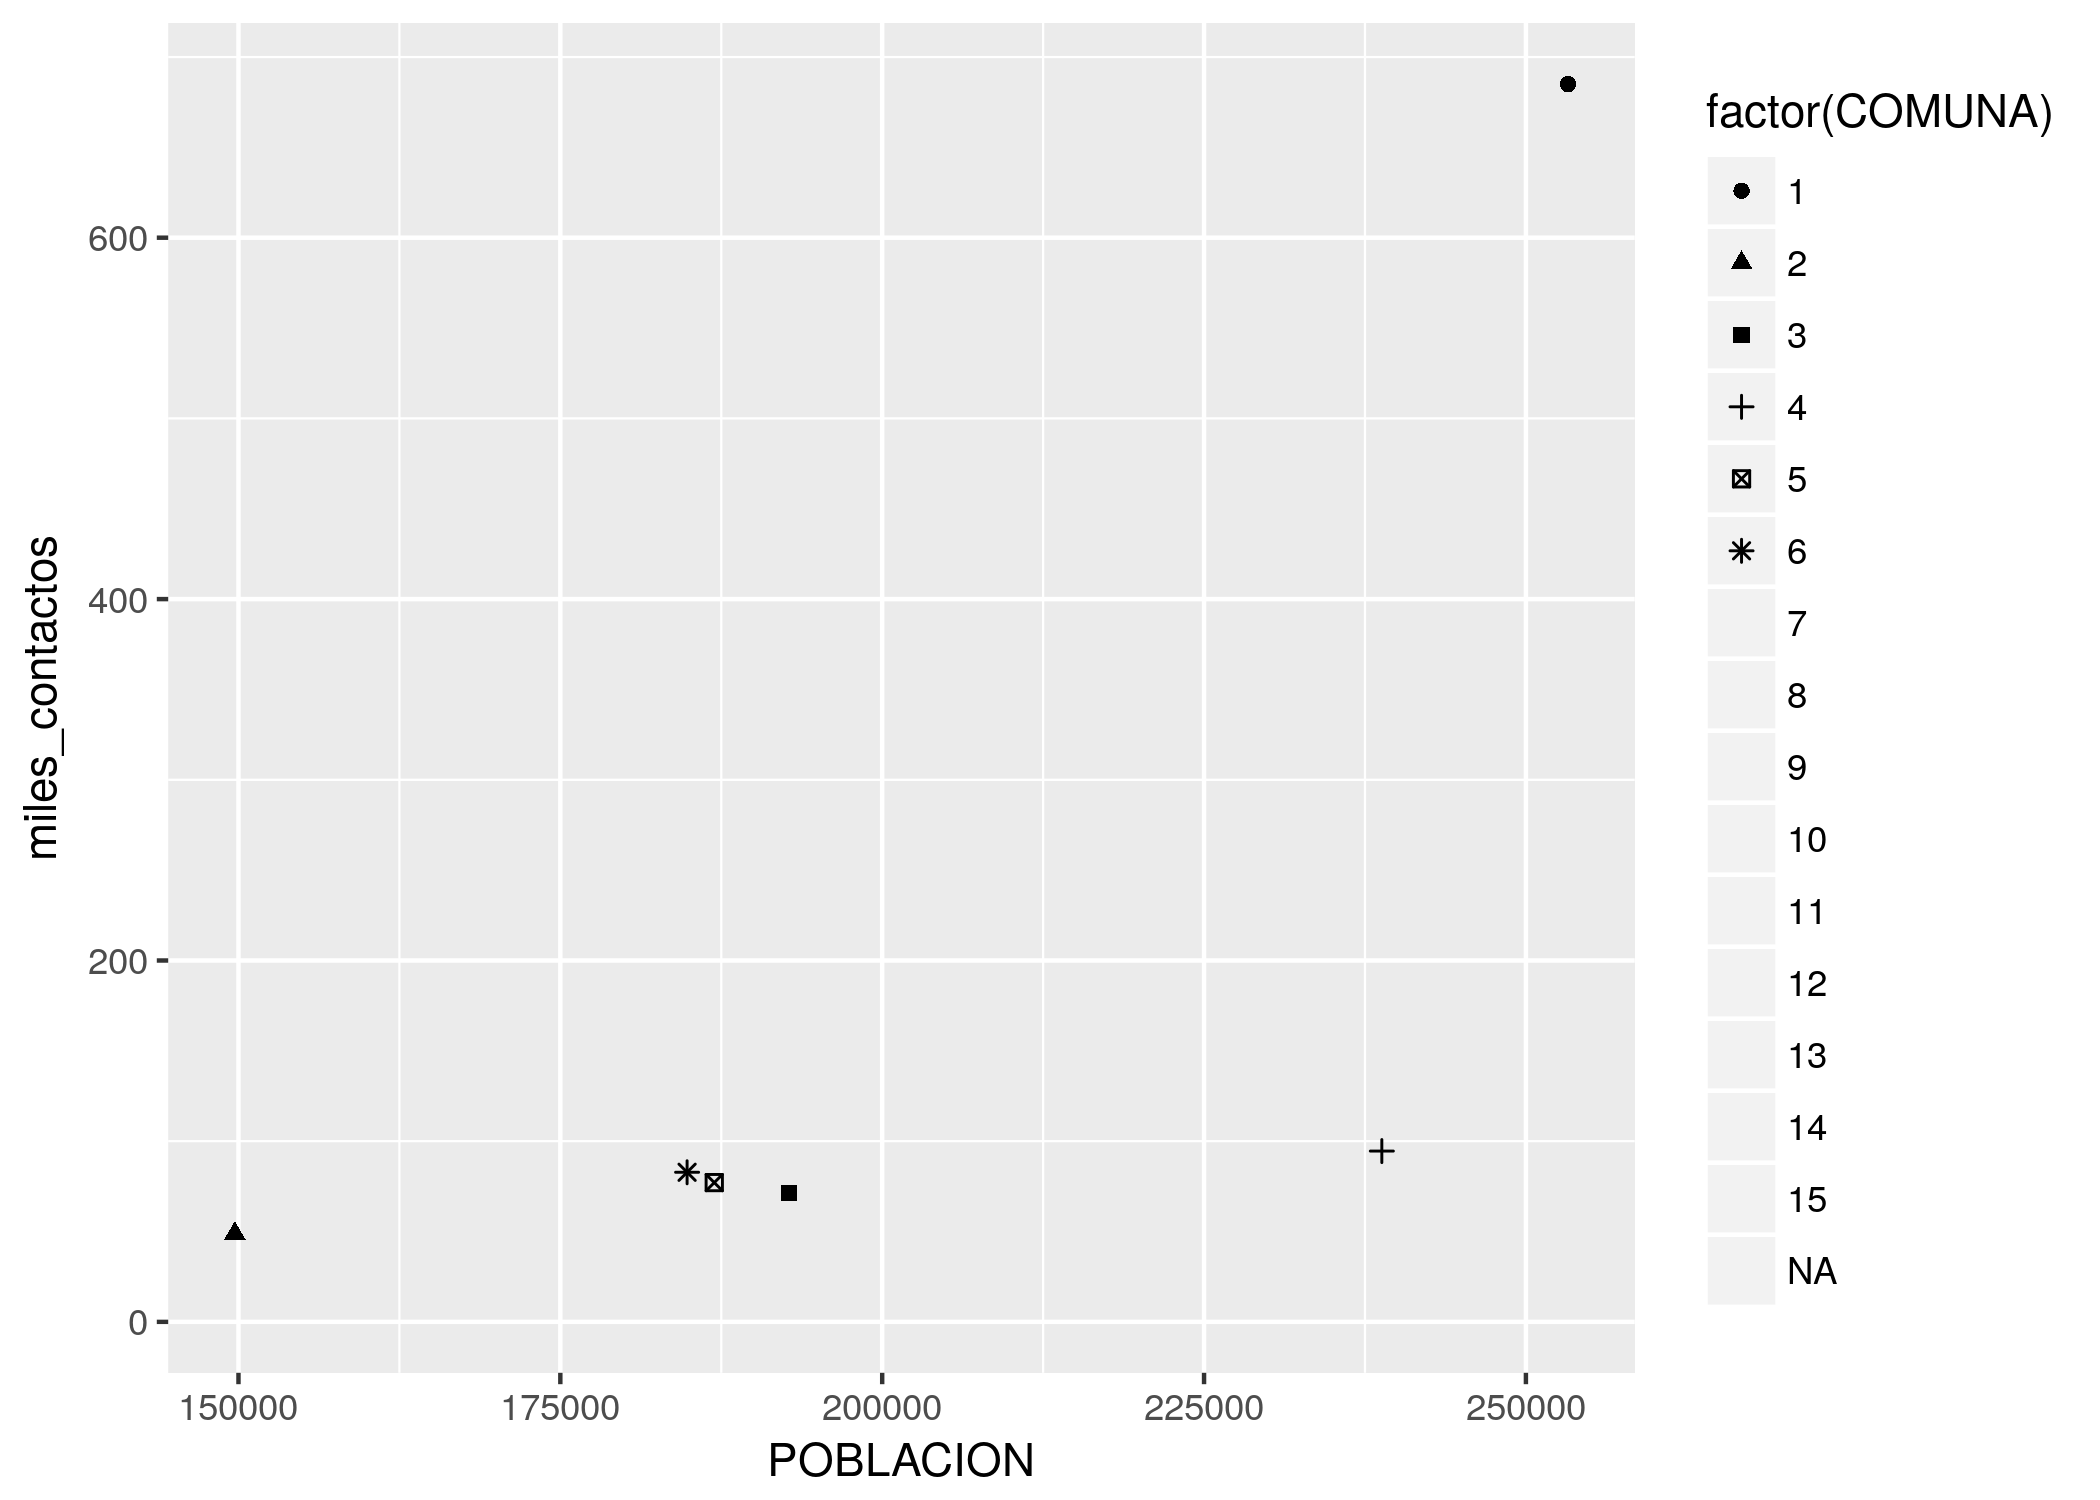
\includegraphics{ciencia_de_datos_para_gente_sociable_files/figure-latex/unnamed-chunk-119-1.pdf}

Hacer una regresión lineal se trata de encontrar la línea que atraviesa
nuestra nube de puntos de modo tal que la suma de las distancias de cada
punto a la línea sea la menor posible. Es un problema matemático que
puede resolverse con distintas técnicas (algebra lineal, geometría, etc)
que no vamos a discutir aquí. Confiaremos en R para hacer los cálculos.

En la relación año - expectativa de vida las distancias entre los puntos
(las observaciones) y la línea (el modelo) son muy pequeñas. Eso indica
que el modelo describe con gran precisión la dinámica de la relación
entre las variables analizadas.

En general, es inusual encontrar una correlación tan nítida entre
variables ``en la vida real'', sobre todo cuando estudiamos procesos
complejos cuyo comportamiento describe patrones más complejos que una
relación lineal pura. No hace falta ir demasiado lejos para encontrar un
ejemplo. Usando el mismo dataset, visualicemos un scatterplot de PBI vs
año, agregando la línea de regresión para:

\begin{Shaded}
\begin{Highlighting}[]
\KeywordTok{ggplot}\NormalTok{(}\DataTypeTok{data =}\NormalTok{ data_arg) }\OperatorTok{+}\StringTok{ }
\StringTok{    }\KeywordTok{geom_point}\NormalTok{(}\KeywordTok{aes}\NormalTok{(}\DataTypeTok{x =}\NormalTok{ año, }\DataTypeTok{y =}\NormalTok{ PBI_PC)) }\OperatorTok{+}
\StringTok{    }\KeywordTok{labs}\NormalTok{(}\DataTypeTok{title =} \StringTok{"Correlación entre PBI y expectativa de vida"}\NormalTok{,}
         \DataTypeTok{subtitle =} \StringTok{"Argentina"}\NormalTok{,}
         \DataTypeTok{y =} \StringTok{"PBI per cápita"}\NormalTok{) }\OperatorTok{+}
\StringTok{    }\KeywordTok{geom_smooth}\NormalTok{(}\KeywordTok{aes}\NormalTok{(}\DataTypeTok{x =}\NormalTok{ año, }\DataTypeTok{y =}\NormalTok{ PBI_PC), }\DataTypeTok{method =} \StringTok{"lm"}\NormalTok{)}
\end{Highlighting}
\end{Shaded}

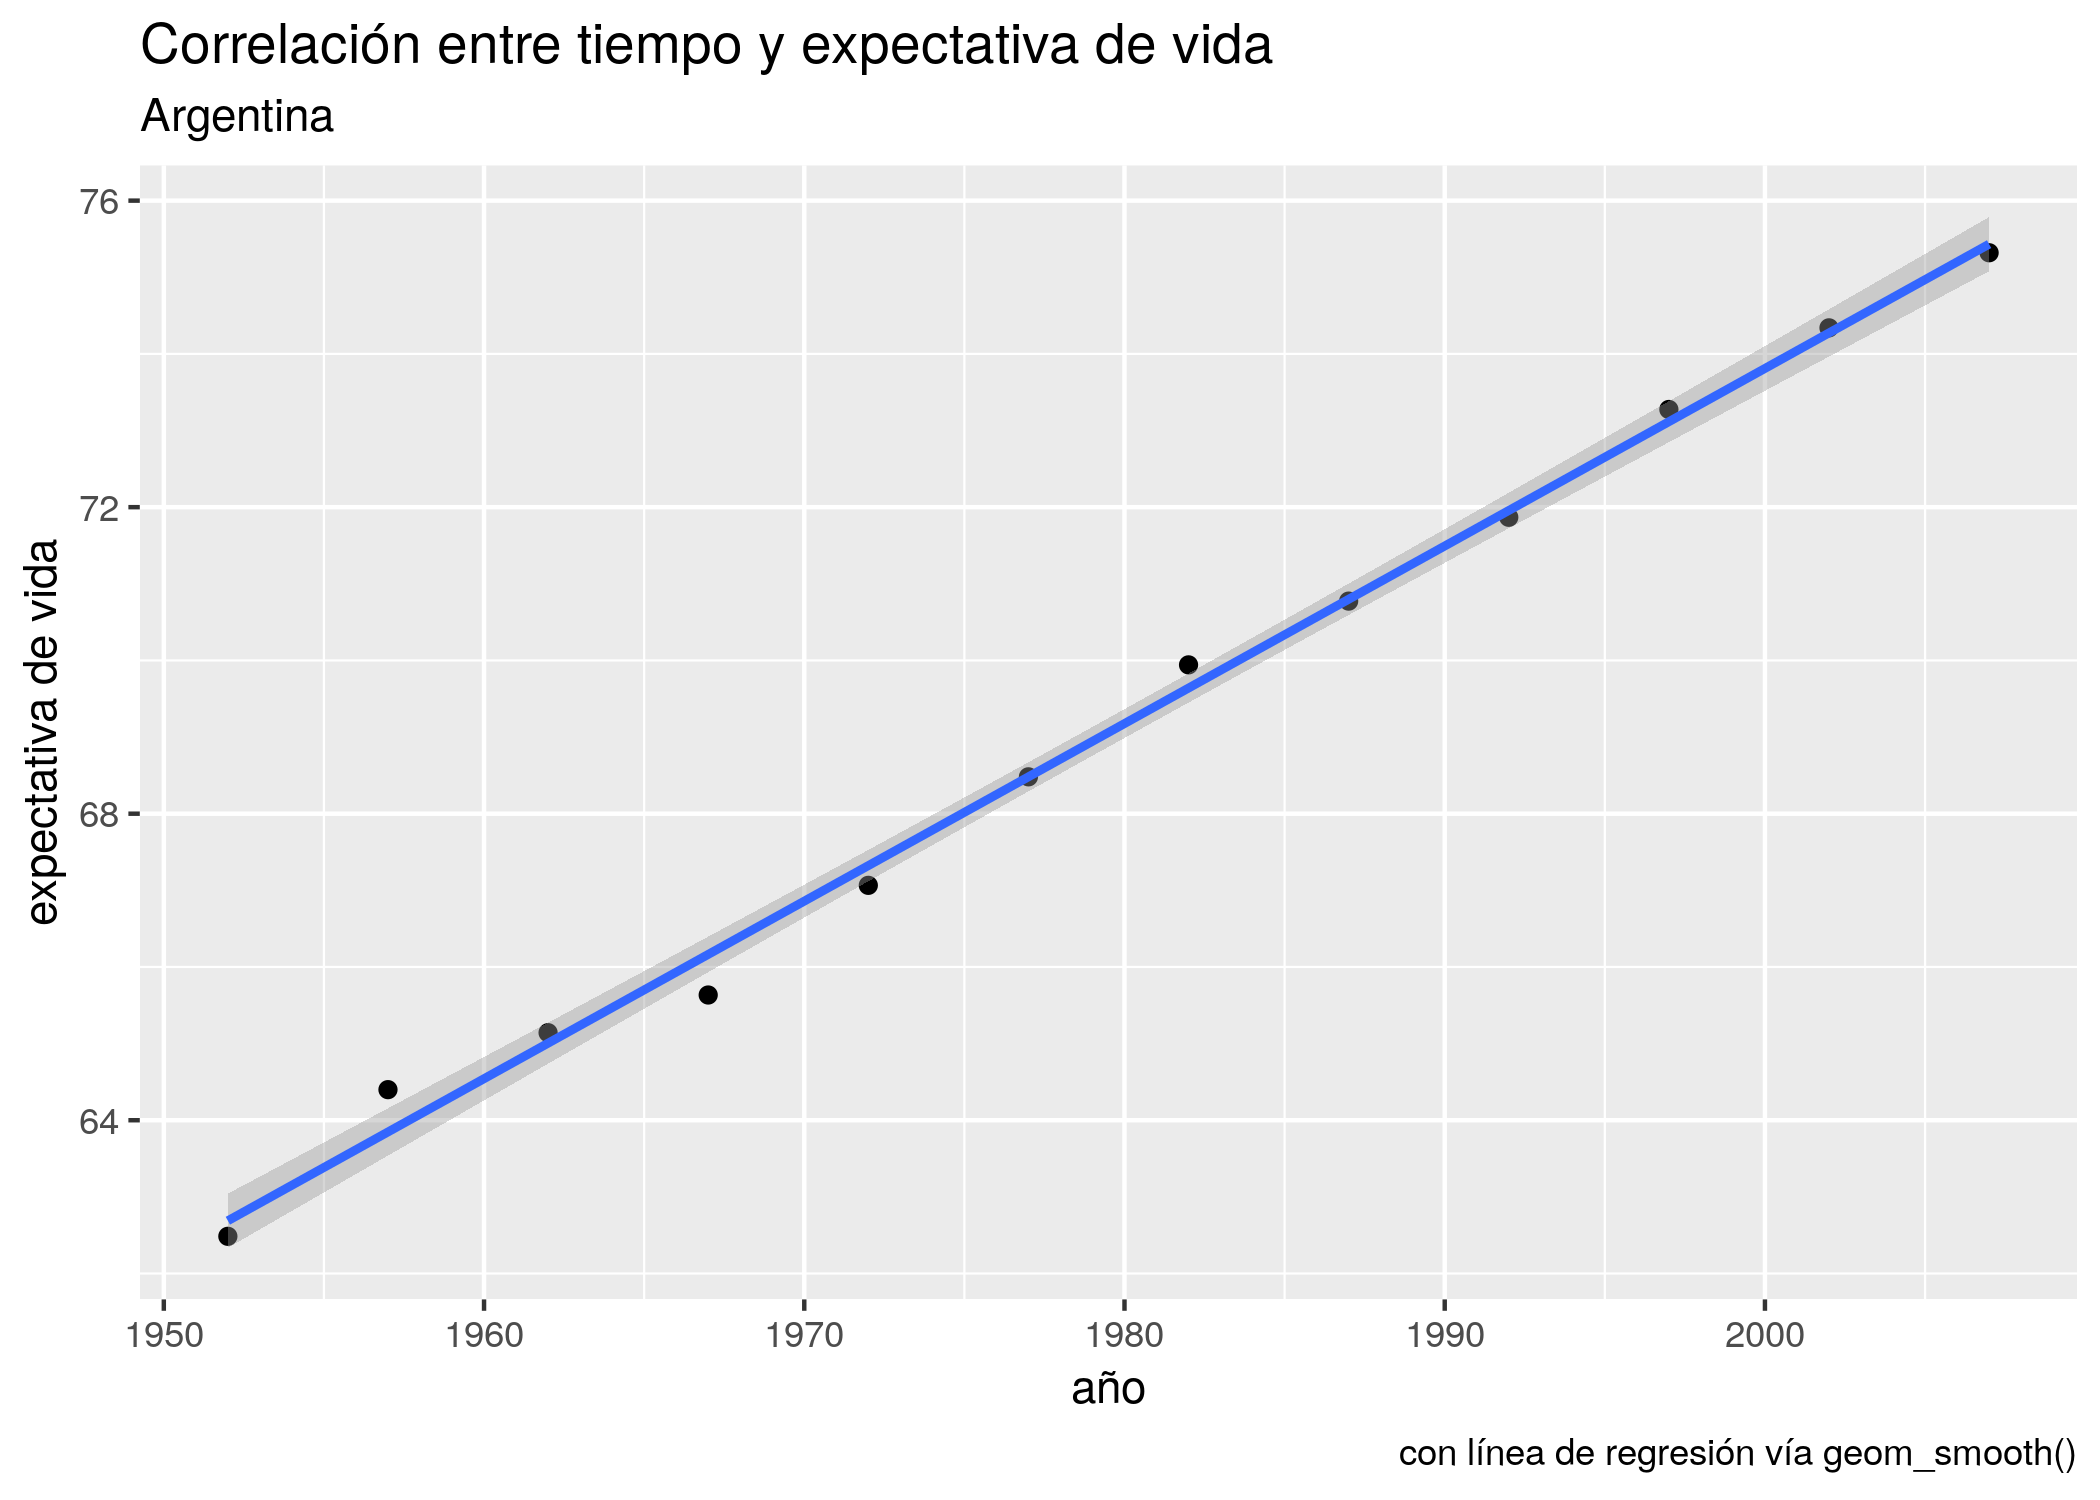
\includegraphics{ciencia_de_datos_para_gente_sociable_files/figure-latex/unnamed-chunk-120-1.pdf}

Sigue siendo evidente una fuerte tendencia lineal, pero las
observaciones ya no se ciñen de forma tan estrecha a la línea idealizada
de la regresión.

Obtengamos el modelo del PBI per cápita de la Argentina en relación al
paso del tiempo:

\begin{Shaded}
\begin{Highlighting}[]
\NormalTok{modelo_PBI <-}\StringTok{ }\KeywordTok{lm}\NormalTok{(PBI_PC }\OperatorTok{~}\StringTok{ }\NormalTok{año, }\DataTypeTok{data =}\NormalTok{ data_arg)}

\NormalTok{modelo_PBI}
\end{Highlighting}
\end{Shaded}

\begin{verbatim}
## 
## Call:
## lm(formula = PBI_PC ~ año, data = data_arg)
## 
## Coefficients:
## (Intercept)          año  
##  -162888.14        86.81
\end{verbatim}

Tal como indicaba el scatterplot, obtuvimos un coeficiente positivo.
Según el modelo, cada año que pasa resulta en un incremento de 86
dólares en el PBI per cápita del país. Sin embargo, sabemos que no todas
las observaciones cumple al pie de la letra con ese incremento. ¿Debería
preocuparnos eso? Una parte importante del análisis basado en
regresiones es revisar las desviaciones, y decidir si ameritan buscar
una explicación. Para ello, lo mejor es empezar por prestar atención a
los residuos.

\subsection{Revolviendo los residuos}\label{revolviendo-los-residuos}

Los residuos, en la jerga estadística, no son otra cosa que las
diferencias encontradas entre el valor que predice un modelo y el valor
observado para una variable. Es decir, el valor para cada punto de
\(y - \widehat{y}\). Los residuos representan el desvío de cada
observación respecto al valor esperado por el modelo.

Cuando los desvíos son pequeños, es decir cuando los residuos son
pequeños, decimos que nuestro modelo se ajusta bien a los datos
observados. Cuando los residuos son grandes ocurre lo contrario, y
quizás deberíamos buscar otros modelos para representar la relación
entre las variables.

Prestemos atención a los residuos de nuestro modelo de PBV vs.~tiempo.
Podemos extraer los residuos usando la función \texttt{residuals()},

\begin{Shaded}
\begin{Highlighting}[]
\NormalTok{residuos <-}\StringTok{ }\KeywordTok{residuals}\NormalTok{(modelo_PBI)}

\NormalTok{residuos}
\end{Highlighting}
\end{Shaded}

\begin{verbatim}
##          1          2          3          4          5          6 
##  -656.9180  -145.4351  -303.1836   182.5450  1138.5722  1340.5021 
##          7          8          9         10         11         12 
##  -174.6855  -466.9699  -732.2809   492.5240 -2111.1755  1436.5051
\end{verbatim}

agregarlos a nuestro dataframe,

\begin{Shaded}
\begin{Highlighting}[]
\NormalTok{data_arg <-}\StringTok{ }\NormalTok{data_arg }\OperatorTok\StringTok{ }\KeywordTok{mutate}\NormalTok{(}\DataTypeTok{residuo_ml =}\NormalTok{ residuos)}
\end{Highlighting}
\end{Shaded}

y visualizarlos comparados con una línea que indica el cero, trazada por
\texttt{geom\_hline()}. Los residuos cercanos a ese valor son los que
corresponden a observaciones a las que el modelo se ajusta bien.

\begin{Shaded}
\begin{Highlighting}[]
\KeywordTok{ggplot}\NormalTok{(data_arg) }\OperatorTok{+}
\StringTok{    }\KeywordTok{geom_point}\NormalTok{(}\KeywordTok{aes}\NormalTok{(}\DataTypeTok{x =}\NormalTok{ año, }\DataTypeTok{y =}\NormalTok{ residuo_ml)) }\OperatorTok{+}
\StringTok{    }\KeywordTok{geom_hline}\NormalTok{(}\DataTypeTok{yintercept =} \DecValTok{0}\NormalTok{, }\DataTypeTok{col =} \StringTok{"blue"}\NormalTok{) }\OperatorTok{+}
\StringTok{    }\KeywordTok{labs}\NormalTok{(}\DataTypeTok{x =} \StringTok{"año"}\NormalTok{, }\DataTypeTok{y =} \StringTok{"residuo del modelo lineal"}\NormalTok{)}
\end{Highlighting}
\end{Shaded}

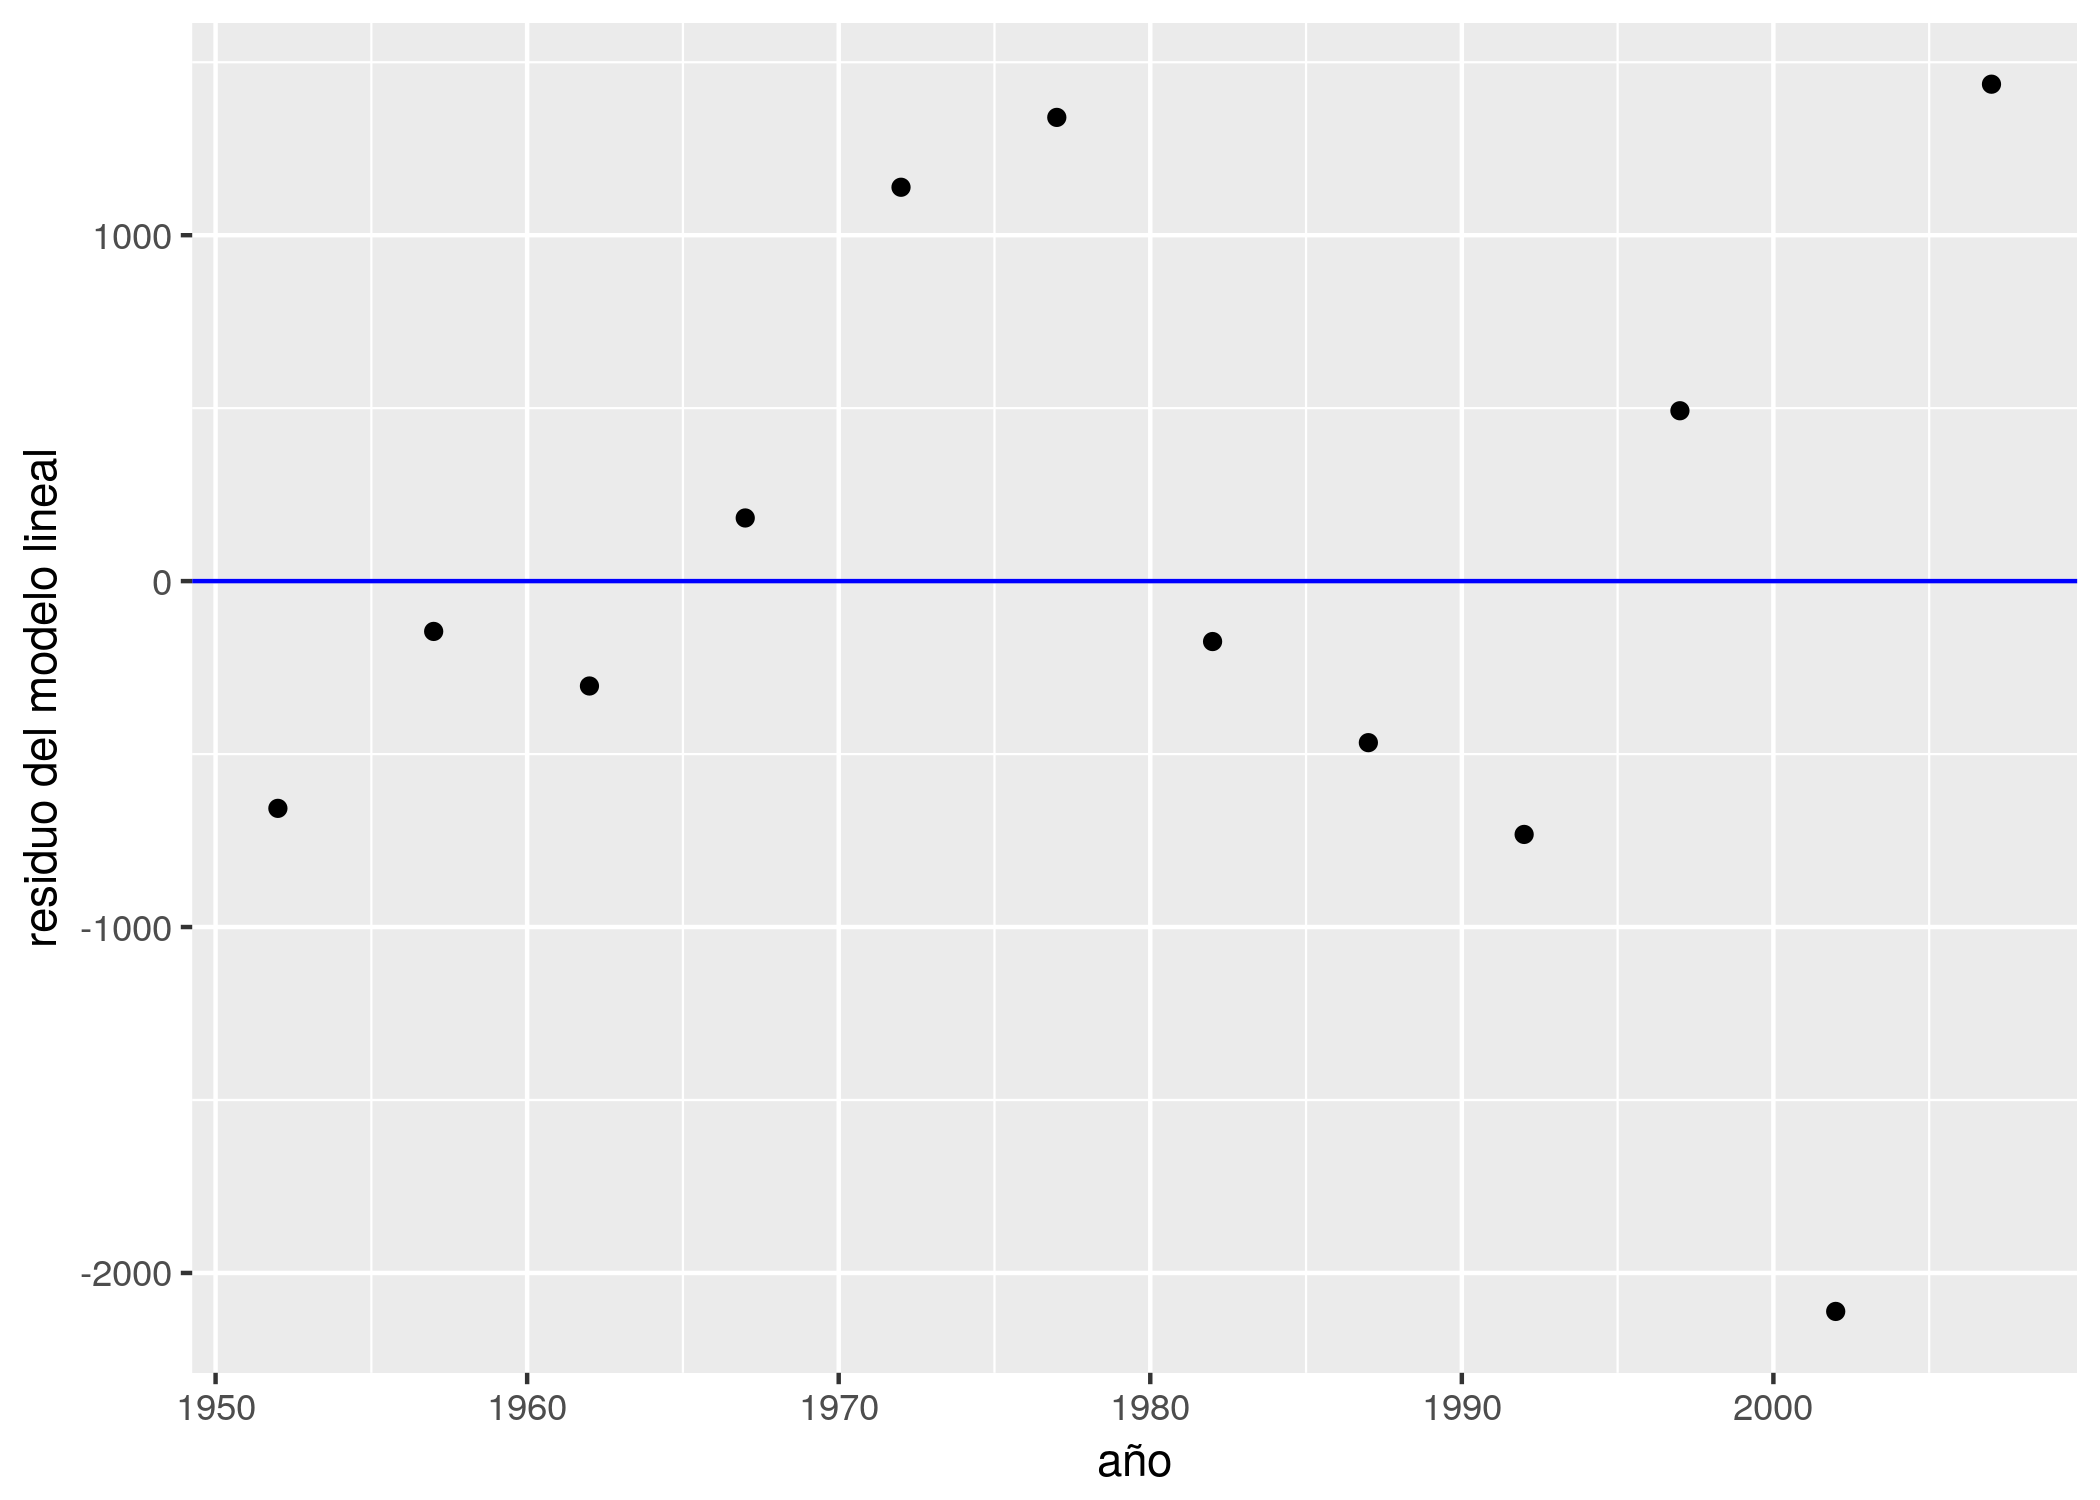
\includegraphics{ciencia_de_datos_para_gente_sociable_files/figure-latex/unnamed-chunk-124-1.pdf}

Siempre podemos esperar una cierta divergencia entre las predicciones y
los valores observados, por lo que los residuos siempre tendrán (en
general) un valor distinto a cero. Lo que quisiéramos ver en un gráfico
como este es que los residuos se distribuyan al azar, sin indicios de
\emph{patrones sistemáticos}. Si así fuere, podemos considerar que
nuestro modelo es adecuado.

¿Cómo determinamos que no exhiben patrones sistemáticos? Una vez mas, se
trata de una evaluación bastante subjetiva, y cada quien estará conforme
dependiendo del contexto y la experiencia previa. Aún así podemos
argumentar en favor de la adecuación del modelo cuando:

\begin{enumerate}
\def\labelenumi{\arabic{enumi}.}
\tightlist
\item
  El promedio de los residuos se aproxima a cero; es decir, que los
  residuos positivos se cancelan con los negativos, promediando cerca de
  cero.
\item
  El valor de los residuos no depende del valor de \(x\); es decir, no
  se observa un crecimiento (o decrecimiento) sistemático de la magnitud
  de los residuos a medida que\(x\) crece
\end{enumerate}

Por lo visto, nuestro modelo cumple con \texttt{1.} pero no con
\texttt{2}, ya que la magnitud de los residuos parece crecer con el paso
de los años. Entre todos los puntos, los mayores transgresores son los
últimos y corresponden a los años 2002 y 2007. El valor del PBI per
cápita observado en 2002 año resultó ser más de 2000 dólares menor al
esperado por el modelo, todo un derrumbe. ¿A qué se debe tanta
discrepancia? Nuestro modelo no tiene la culpa, es que la realidad tiene
sus bemoles. A fines del 2001 la Argentina sufrió la peor crisis
financiera de su historia, factor que explica la brusca caída del PBI
que revirtió la tendencia al crecimiento de décadas anteriores. Una
función que aún no habíamos usado, \texttt{geom\_line()}, nos va a
permitir trazar una línea que siga el PBI a lo largo de los años, y otra
novedad, \texttt{geom\_vline()}, se encargará de agregar una línea
vertical que señale el año de la crisis:

\begin{Shaded}
\begin{Highlighting}[]
\KeywordTok{ggplot}\NormalTok{(data_arg) }\OperatorTok{+}\StringTok{ }
\StringTok{    }\KeywordTok{geom_line}\NormalTok{(}\KeywordTok{aes}\NormalTok{(}\DataTypeTok{x =}\NormalTok{ año, }\DataTypeTok{y =}\NormalTok{ PBI_PC)) }\OperatorTok{+}
\StringTok{    }\KeywordTok{geom_vline}\NormalTok{(}\KeywordTok{aes}\NormalTok{(}\DataTypeTok{xintercept =} \DecValTok{2001}\NormalTok{), }\DataTypeTok{color =} \StringTok{"red"}\NormalTok{) }\OperatorTok{+}
\StringTok{    }\KeywordTok{labs}\NormalTok{(}\DataTypeTok{title =} \StringTok{"Evolución del PBI en la Argentina"}\NormalTok{,}
         \DataTypeTok{y =} \StringTok{"PBI per cápita"}\NormalTok{,}
         \DataTypeTok{caption =} \StringTok{"La línea roja indica la ocurrencia de la crisis del 2001"}\NormalTok{)}
\end{Highlighting}
\end{Shaded}

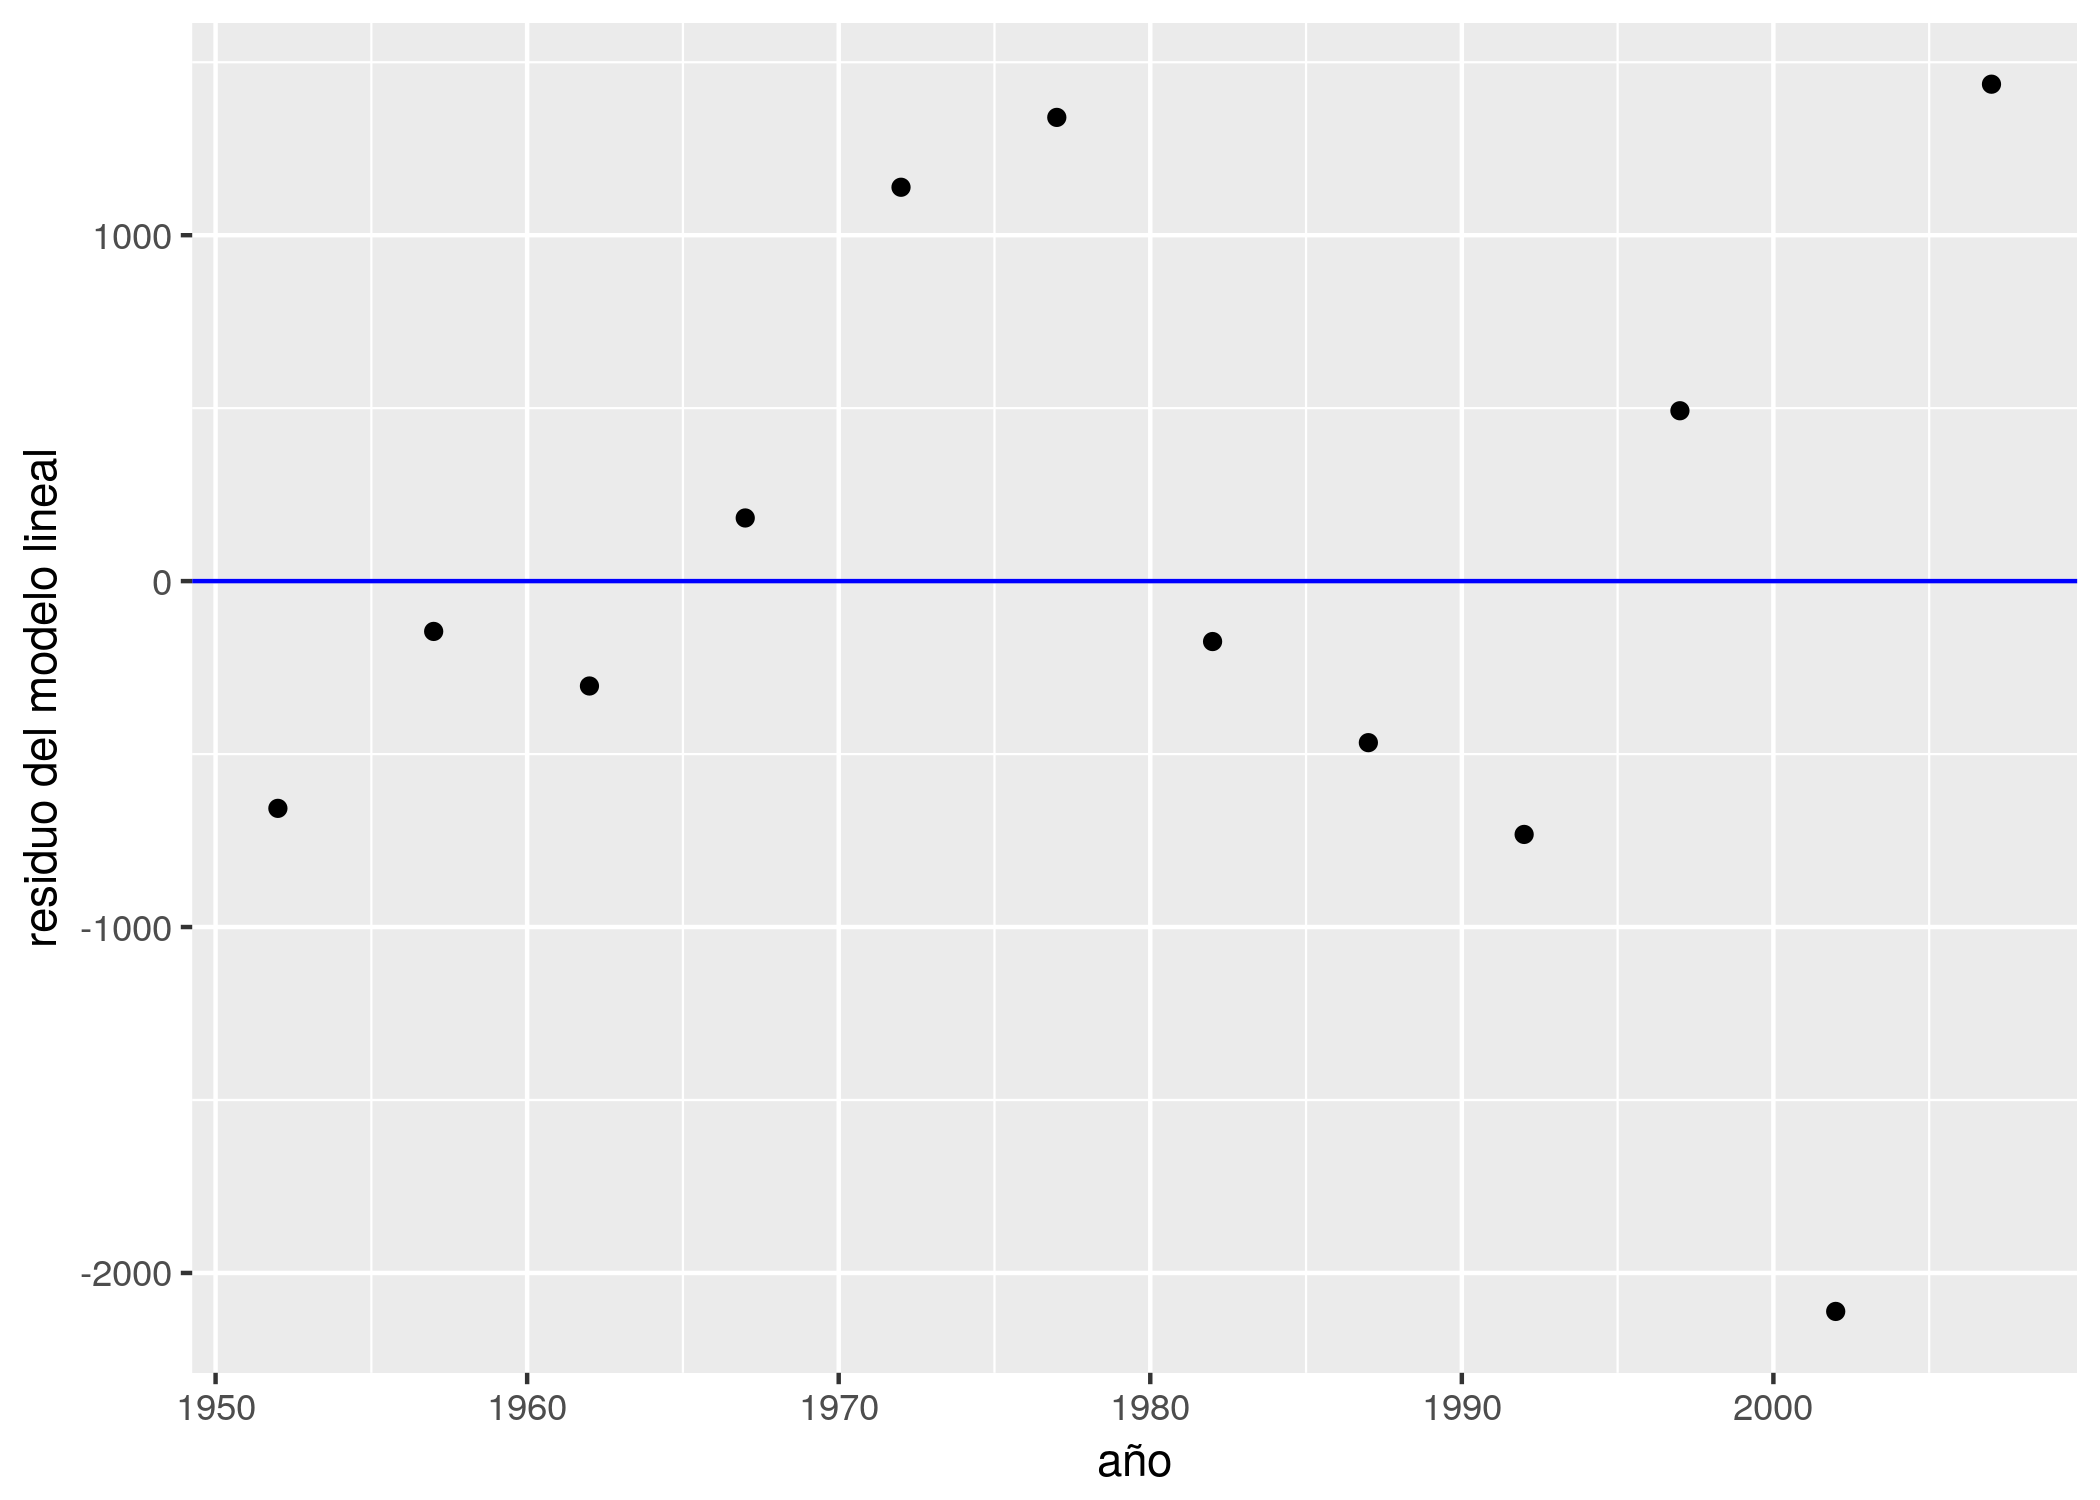
\includegraphics{ciencia_de_datos_para_gente_sociable_files/figure-latex/unnamed-chunk-125-1.pdf}

Es claro que el modelo se beneficiaría de poder tener en cuenta la
irrupción de las crisis en el país. Esto se lograría agregando una
variable categórica para cada año, que indique si se trata de un período
de crisis. En ese caso, seria un modelo de regresión lineal múltiple
(con más de una variable explicativa), incorporando una variable
explicativa numérica y otra categórica. Que lástima que nuestro dataset
no incluye la variable de las crisis financieras. Si quisiéramos mejorar
nuestro modelo con esa información, no nos quedaría mas remedio que
salir a buscar los datos. Con suerte, alguien los habrá recopilado por
nosotros, y si no, tendríamos que hacerlo por nuestra cuenta. ¡La
investigación es un sacerdocio!

En aras de la simplicidad, sigamos practicando con los datos
disponibles.

\subsection{Regresión con una variable
categórica}\label{regresion-con-una-variable-categorica}

El dataset con datos del mundo provisto por Gapminder incluye dos
variables categóricas: país y continente. Con 142 países representados,
podemos descartar a la primera como variable para realizar un modelo
-recordemos que para entender la interrelación de variables, cuantas
menos involucremos mejor. Los cinco continentes habitados representan un
conjunto mucho más práctico, por lo que la pregunta será ``¿Cuánto
incide el continente en la expectativa de vida de los países?''

Comencemos por explorar los datos tomando las observaciones más
recientes, las de 2007.

\begin{Shaded}
\begin{Highlighting}[]
\NormalTok{data_mundial_}\DecValTok{2007}\NormalTok{ <-}\StringTok{ }\NormalTok{data_mundial }\OperatorTok\StringTok{ }\KeywordTok{filter}\NormalTok{(año }\OperatorTok{==}\StringTok{ }\DecValTok{2007}\NormalTok{)}

\KeywordTok{ggplot}\NormalTok{(}\DataTypeTok{data =}\NormalTok{ data_mundial_}\DecValTok{2007}\NormalTok{) }\OperatorTok{+}
\StringTok{    }\KeywordTok{geom_point}\NormalTok{(}\KeywordTok{aes}\NormalTok{(}\DataTypeTok{x =}\NormalTok{ continente, }\DataTypeTok{y =}\NormalTok{ expVida, }\DataTypeTok{color =}\NormalTok{ continente)) }\OperatorTok{+}
\StringTok{    }\KeywordTok{labs}\NormalTok{(}\DataTypeTok{title =} \StringTok{"Expectativa de vida por continente"}\NormalTok{,}
         \DataTypeTok{y =} \StringTok{"expectativa de vida"}\NormalTok{)}
\end{Highlighting}
\end{Shaded}

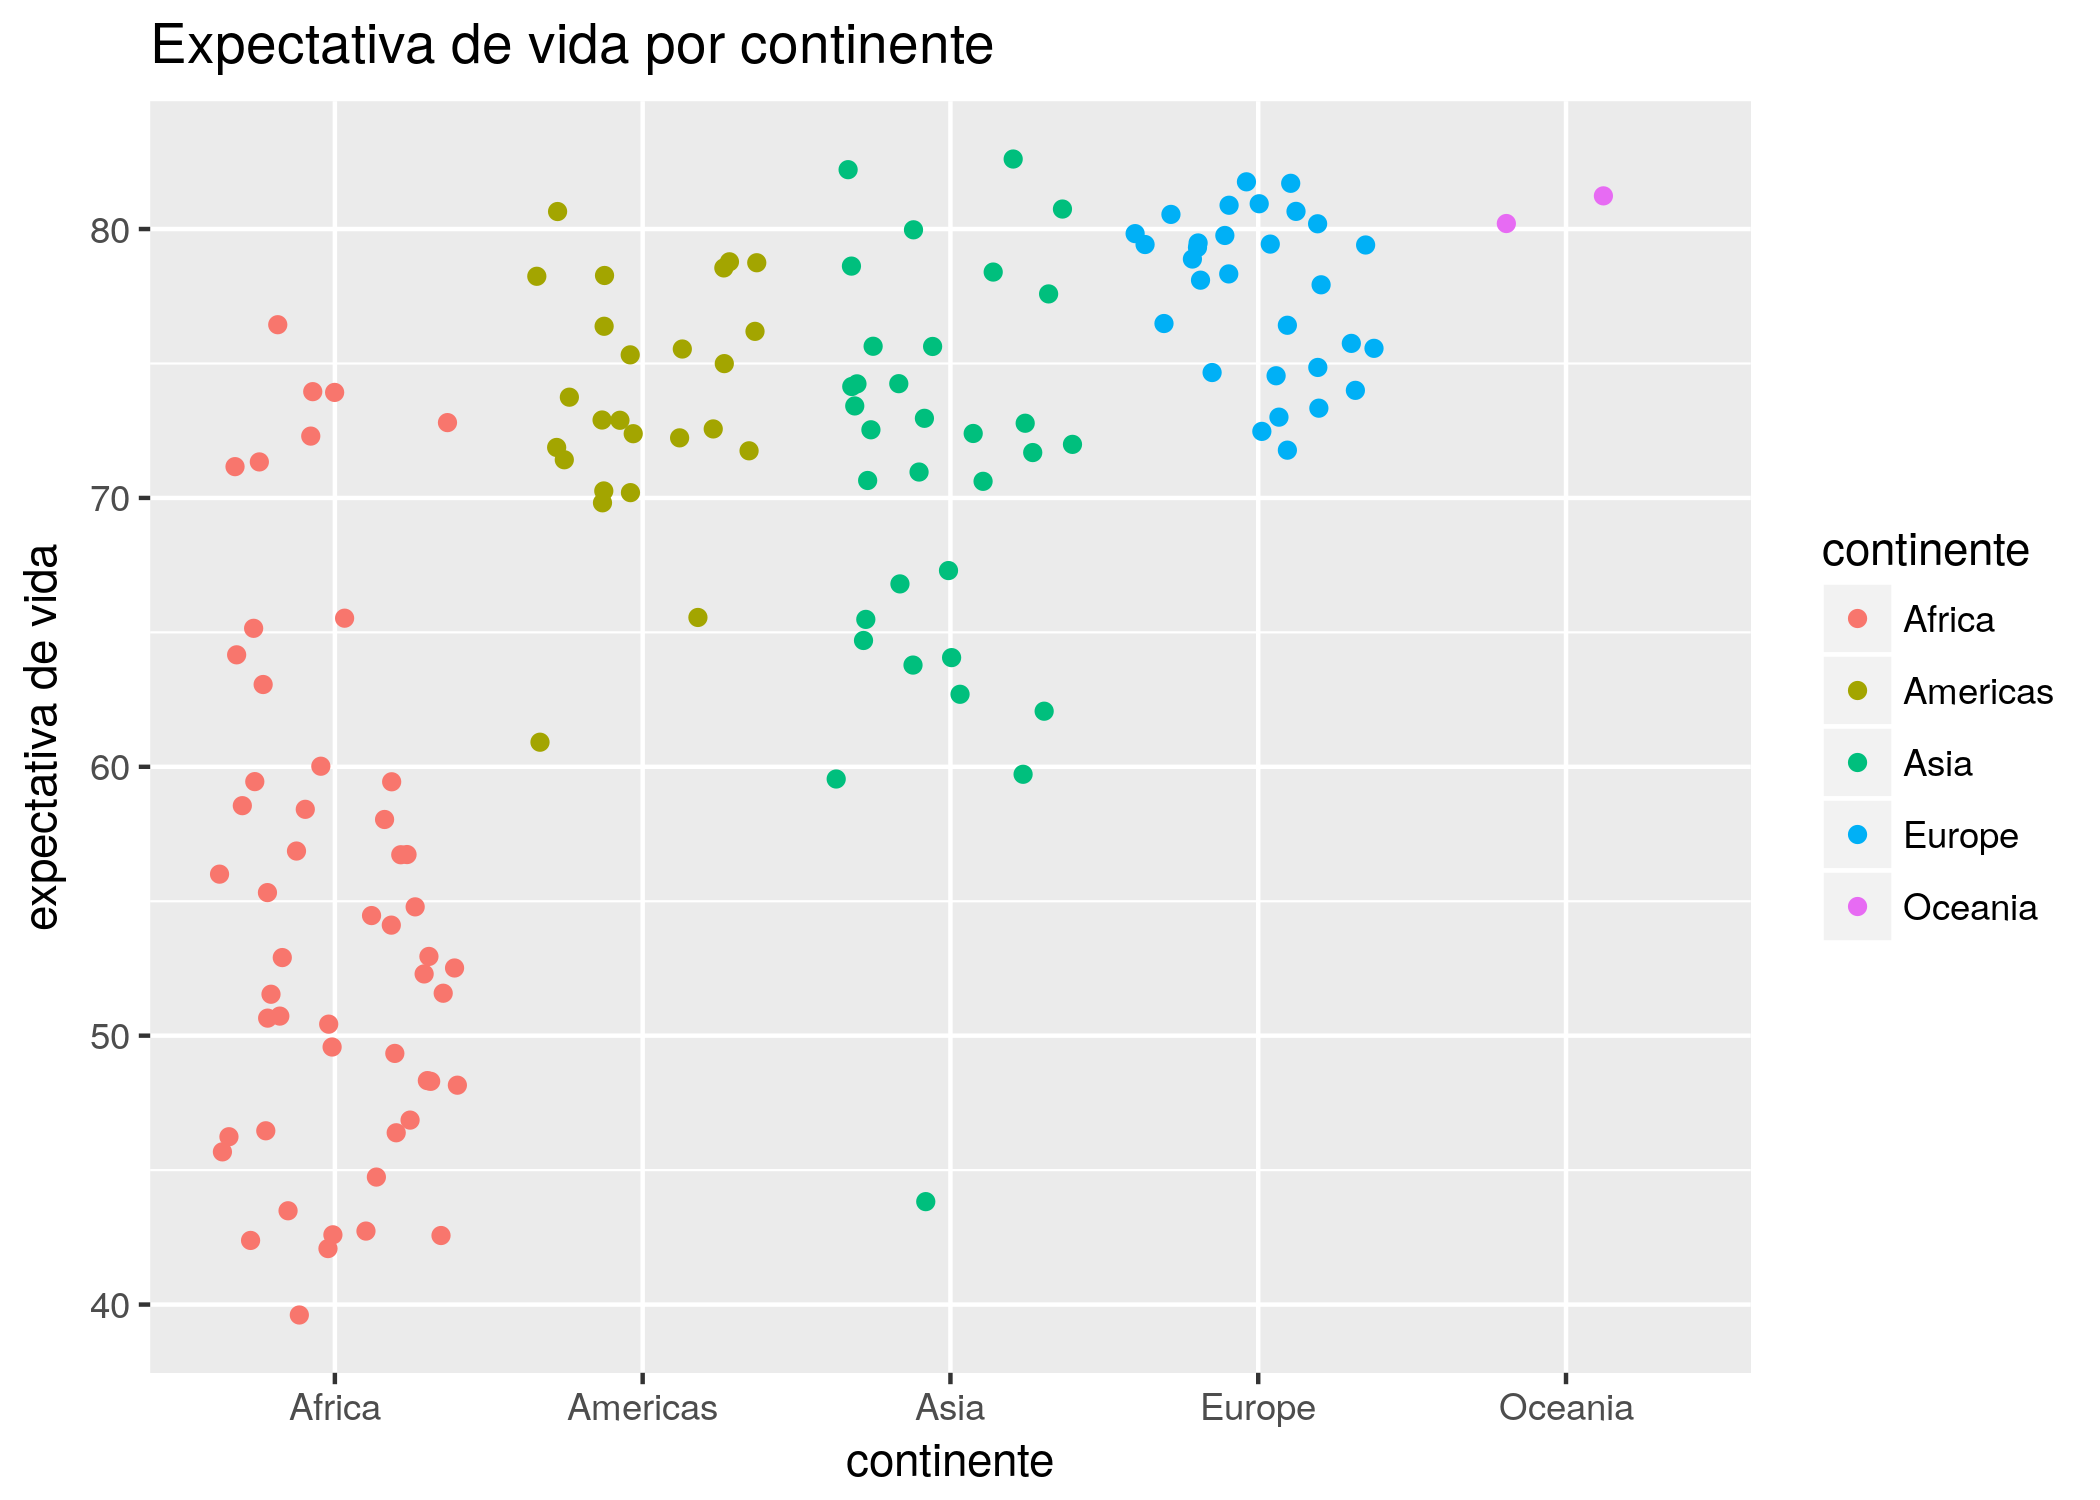
\includegraphics{ciencia_de_datos_para_gente_sociable_files/figure-latex/unnamed-chunk-126-1.pdf}

Ya podemos vislumbrar que el continente incide en la expectativa de
vida, con África sufriendo los números más bajos. La profusión de puntos
hace que muchos terminen superpuestos, haciendo imposible determinar
cuántos ocupan cada posición (un problema llamado \emph{overplotting} en
inglés). Una variante de \texttt{geom\_point()} llamada
\texttt{geom\_jitter()} resuelve este problema al ``sacudir'' los
puntos, sumando a cada uno un pequeño valor al azar para que se separe
de los que comparten su posición. Es un buen ejemplo de la paradoja por
la cual reducir la precisión de la información a veces permite entender
mejor lo que está ocurriendo. Usamos \texttt{geom\_jitter()} igual que
\texttt{geom\_point()}:

\begin{Shaded}
\begin{Highlighting}[]
\KeywordTok{ggplot}\NormalTok{(}\DataTypeTok{data =}\NormalTok{ data_mundial_}\DecValTok{2007}\NormalTok{) }\OperatorTok{+}
\StringTok{    }\KeywordTok{geom_jitter}\NormalTok{(}\KeywordTok{aes}\NormalTok{(}\DataTypeTok{x =}\NormalTok{ continente, }\DataTypeTok{y =}\NormalTok{ expVida, }\DataTypeTok{color =}\NormalTok{ continente)) }\OperatorTok{+}
\StringTok{    }\KeywordTok{labs}\NormalTok{(}\DataTypeTok{title =} \StringTok{"Expectativa de vida por continente"}\NormalTok{,}
         \DataTypeTok{y =} \StringTok{"expectativa de vida"}\NormalTok{)}
\end{Highlighting}
\end{Shaded}

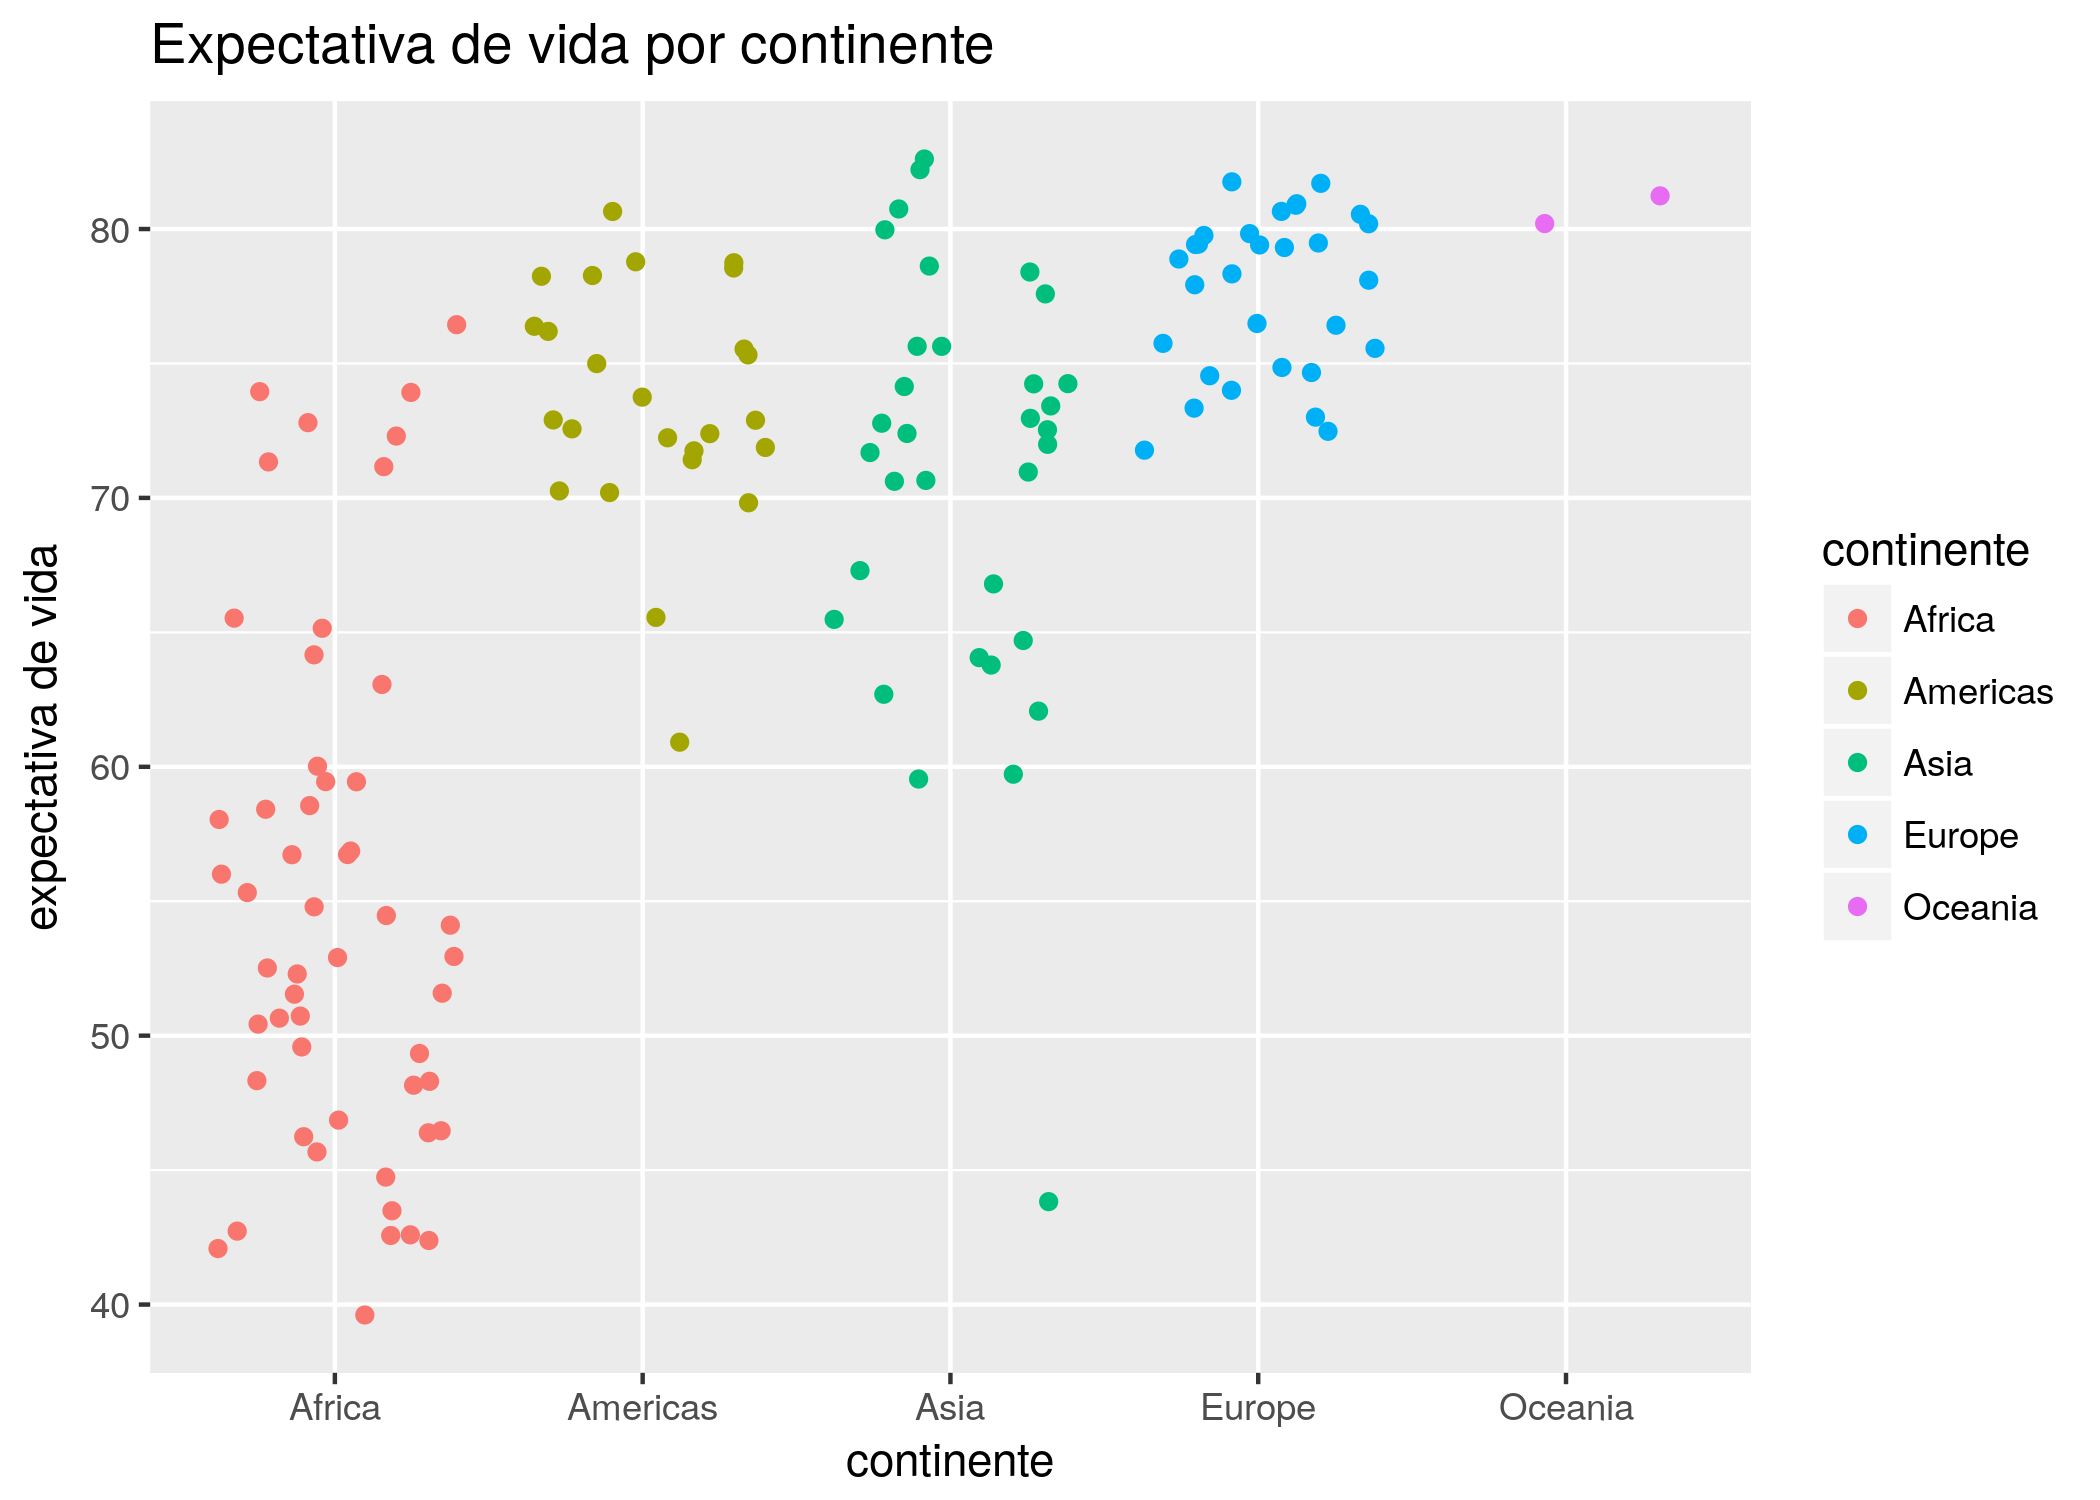
\includegraphics{ciencia_de_datos_para_gente_sociable_files/figure-latex/unnamed-chunk-127-1.pdf}

Algún ojo avizor habrá notado que la clasificación por color no es
necesaria, ya el continente ya está señalado por su posición en el exe
de las \texttt{x}. El color cumple aquí una función más que nada
cosmética, en pos de hacer al gráfico maś atractivo a la vista.

También podemos visualizar la diferencia de distribución de expectactiva
de vida de los países, con un histograma facetado por continente:

\begin{Shaded}
\begin{Highlighting}[]
\KeywordTok{ggplot}\NormalTok{(}\DataTypeTok{data =}\NormalTok{ data_mundial_}\DecValTok{2007}\NormalTok{) }\OperatorTok{+}
\StringTok{    }\KeywordTok{geom_histogram}\NormalTok{(}\KeywordTok{aes}\NormalTok{(}\DataTypeTok{x =}\NormalTok{ expVida, }\DataTypeTok{fill =}\NormalTok{ continente)) }\OperatorTok{+}
\StringTok{    }\KeywordTok{facet_wrap}\NormalTok{(}\OperatorTok{~}\NormalTok{continente) }\OperatorTok{+}
\StringTok{    }\KeywordTok{labs}\NormalTok{(}\DataTypeTok{title =} \StringTok{"Expectativa de vida por continente"}\NormalTok{,}
         \DataTypeTok{subtitle =} \StringTok{"histogramas"}\NormalTok{,}
        \DataTypeTok{x =} \StringTok{"expectativa de vida"}\NormalTok{,}
        \DataTypeTok{y =} \StringTok{"cantidad"}\NormalTok{)}
\end{Highlighting}
\end{Shaded}

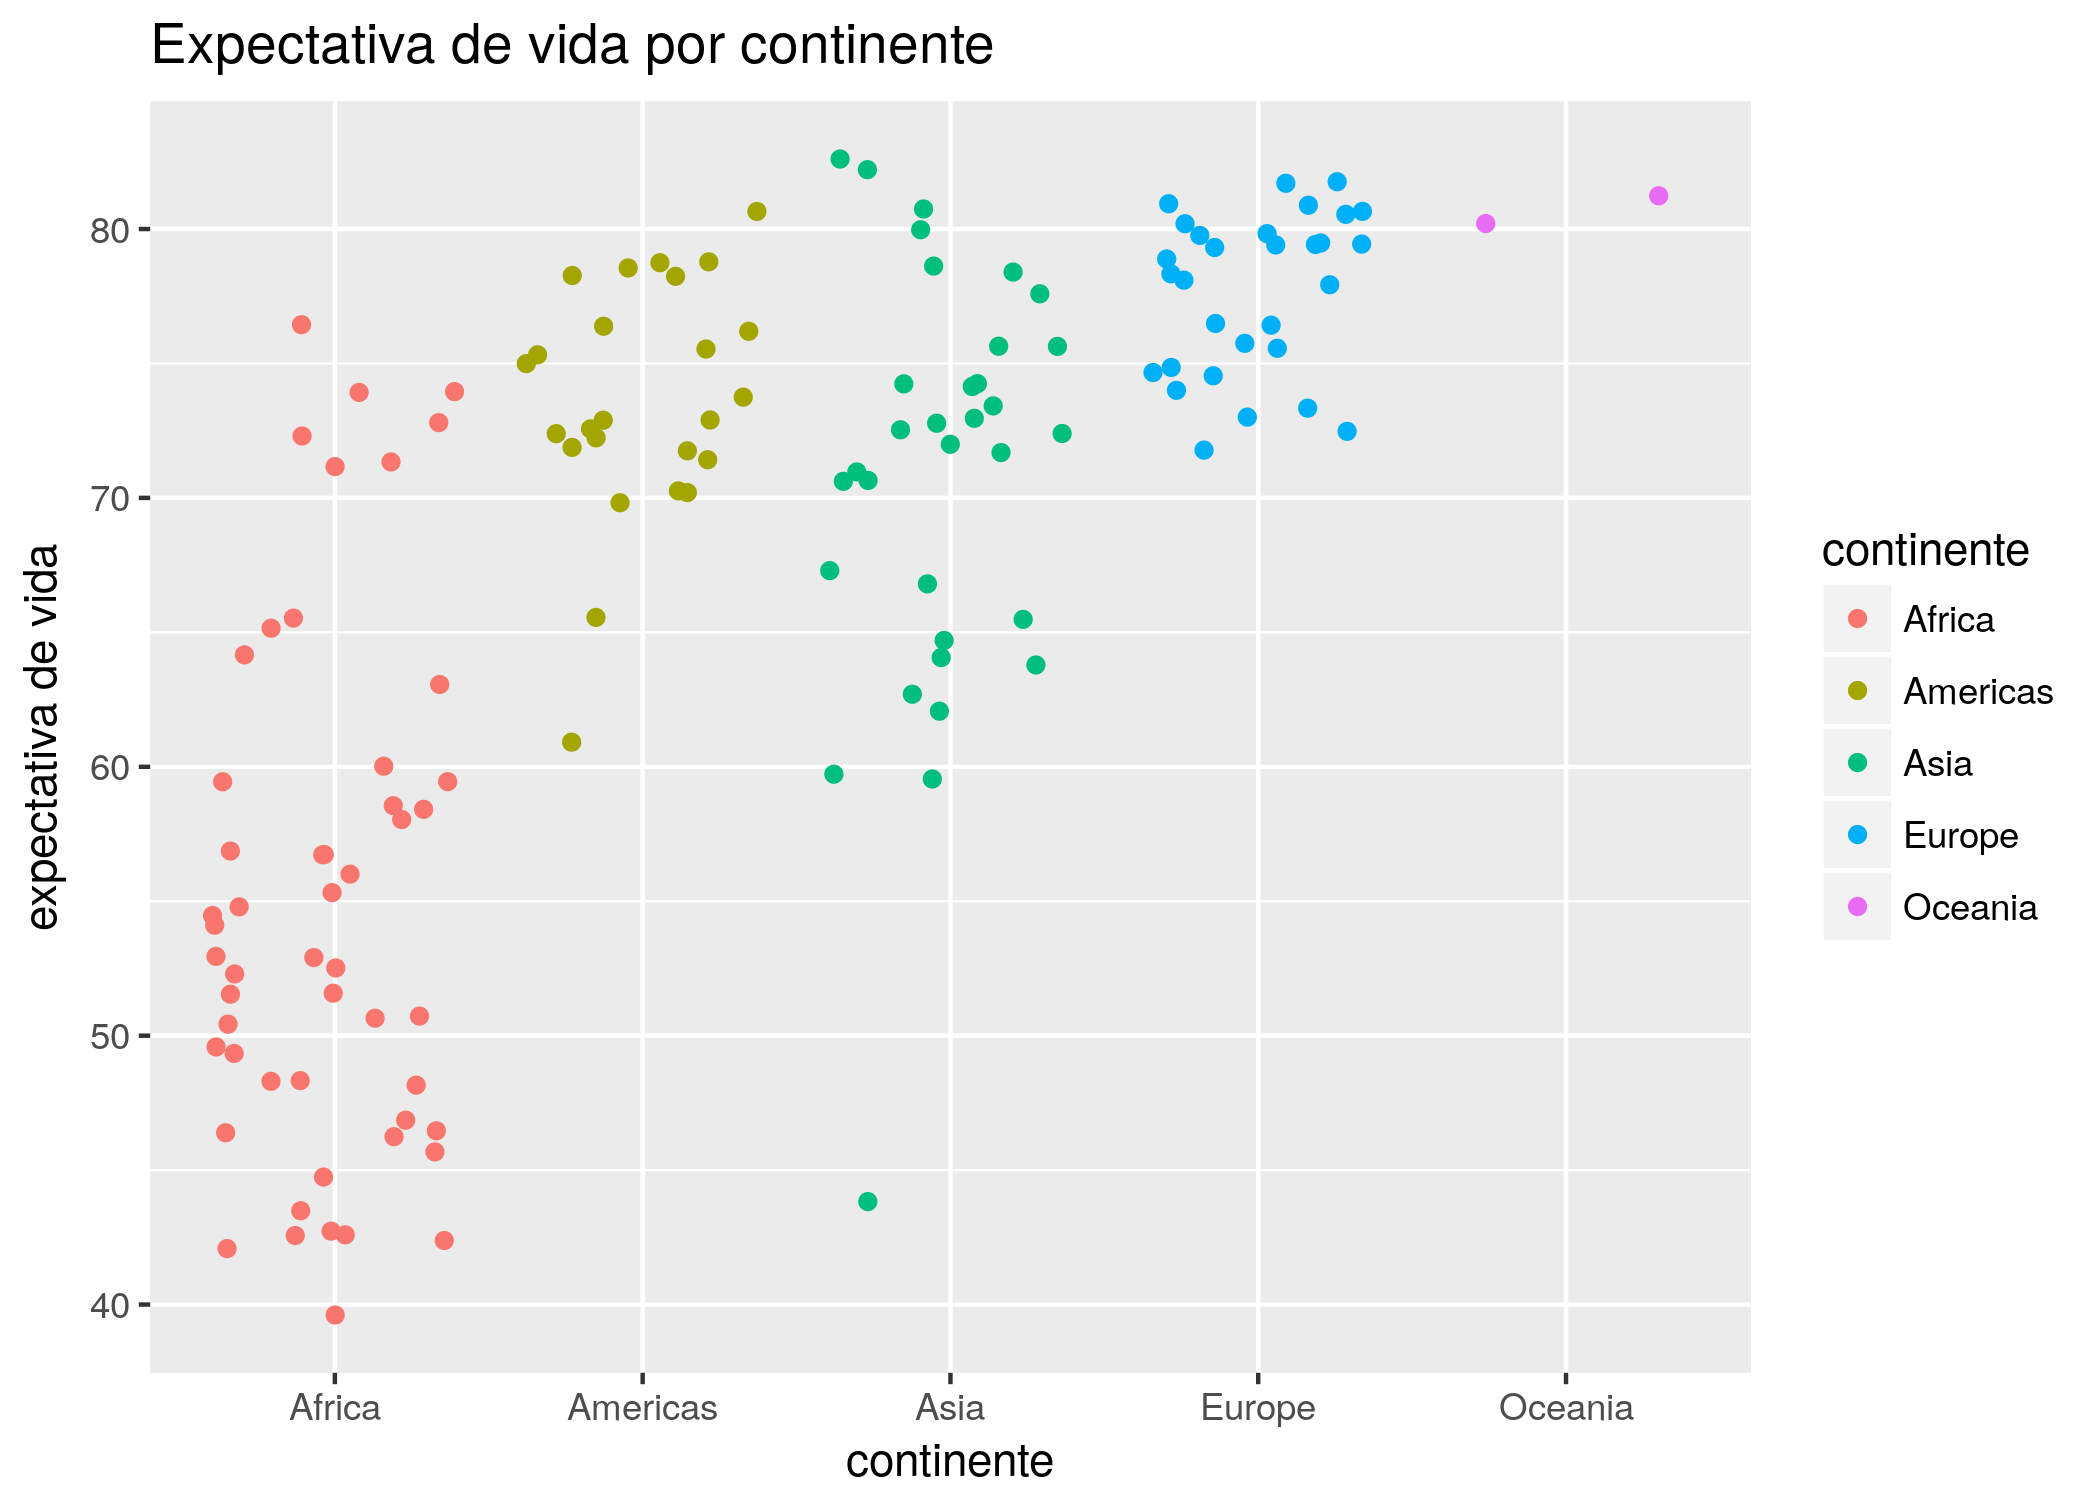
\includegraphics{ciencia_de_datos_para_gente_sociable_files/figure-latex/unnamed-chunk-128-1.pdf}

Bien, estamos convencidos de que hay una relación entre continente y
expectativa de vida, aunque no la hemos cuantificado. Para eso,
recurrimos a una regresión lineal con variable expicativa categórica. Se
obtiene de la misma manera que antes, no hay cambios en la forma de
invocar \texttt{lm()} por el hecho de que la variabe ahora sea
categórica en vez de numérica.

\begin{Shaded}
\begin{Highlighting}[]
\NormalTok{modelo_exp_continente <-}\StringTok{ }\KeywordTok{lm}\NormalTok{(expVida }\OperatorTok{~}\StringTok{ }\NormalTok{continente, }\DataTypeTok{data =}\NormalTok{ data_mundial_}\DecValTok{2007}\NormalTok{)}


\NormalTok{modelo_exp_continente}
\end{Highlighting}
\end{Shaded}

\begin{verbatim}
## 
## Call:
## lm(formula = expVida ~ continente, data = data_mundial_2007)
## 
## Coefficients:
##        (Intercept)  continenteAmericas      continenteAsia  
##              54.81               18.80               15.92  
##   continenteEurope   continenteOceania  
##              22.84               25.91
\end{verbatim}

¿Qué ocurrió aquí? \texttt{lm()} inspeccionó el contenido de la variable
``continente'' y encontró cinco niveles o categorías. Tomó el primero en
orden alfabético, ``Africa'' como línea de base. El primer coeficiente
de la regresión (la intersección) es el promedio de la expectativa de
vida en África. Para cada una de las categorías restantes, el
coeficiente representa la diferencia respecto a África de la expectativa
de vida promedio en cada uno de los otros continentes. He allí la
cuantificación: para un país en las Américas, podemos esperar -en
promedio- una expectativa de vida que supera en 18.8 años la de los
paises africanos. Para un país en Asia, son 15.92 los años adicionales,
y así.

Prestemos atención a los residuos. Agregamos al dataframe una columna
con el residuo para cada observación,

\begin{Shaded}
\begin{Highlighting}[]
\NormalTok{data_mundial_}\DecValTok{2007}\NormalTok{ <-}\StringTok{ }\NormalTok{data_mundial_}\DecValTok{2007} \OperatorTok\StringTok{ }
\StringTok{    }\KeywordTok{mutate}\NormalTok{(}\DataTypeTok{residuo_ml =} \KeywordTok{residuals}\NormalTok{(modelo_exp_continente))}
\end{Highlighting}
\end{Shaded}

y graficamos la dispersión de los residuos en torno a cero, el valor
ideal:

\begin{Shaded}
\begin{Highlighting}[]
\KeywordTok{ggplot}\NormalTok{(data_mundial_}\DecValTok{2007}\NormalTok{) }\OperatorTok{+}
\StringTok{    }\KeywordTok{geom_jitter}\NormalTok{(}\KeywordTok{aes}\NormalTok{(}\DataTypeTok{x =}\NormalTok{ continente, }\DataTypeTok{y =}\NormalTok{ residuo_ml), }\DataTypeTok{width =} \FloatTok{0.1}\NormalTok{) }\OperatorTok{+}
\StringTok{    }\KeywordTok{geom_hline}\NormalTok{(}\DataTypeTok{yintercept =} \DecValTok{0}\NormalTok{, }\DataTypeTok{col =} \StringTok{"blue"}\NormalTok{) }\OperatorTok{+}
\StringTok{    }\KeywordTok{labs}\NormalTok{(}\DataTypeTok{x =} \StringTok{"año"}\NormalTok{, }\DataTypeTok{y =} \StringTok{"residuo del modelo lineal"}\NormalTok{)}
\end{Highlighting}
\end{Shaded}

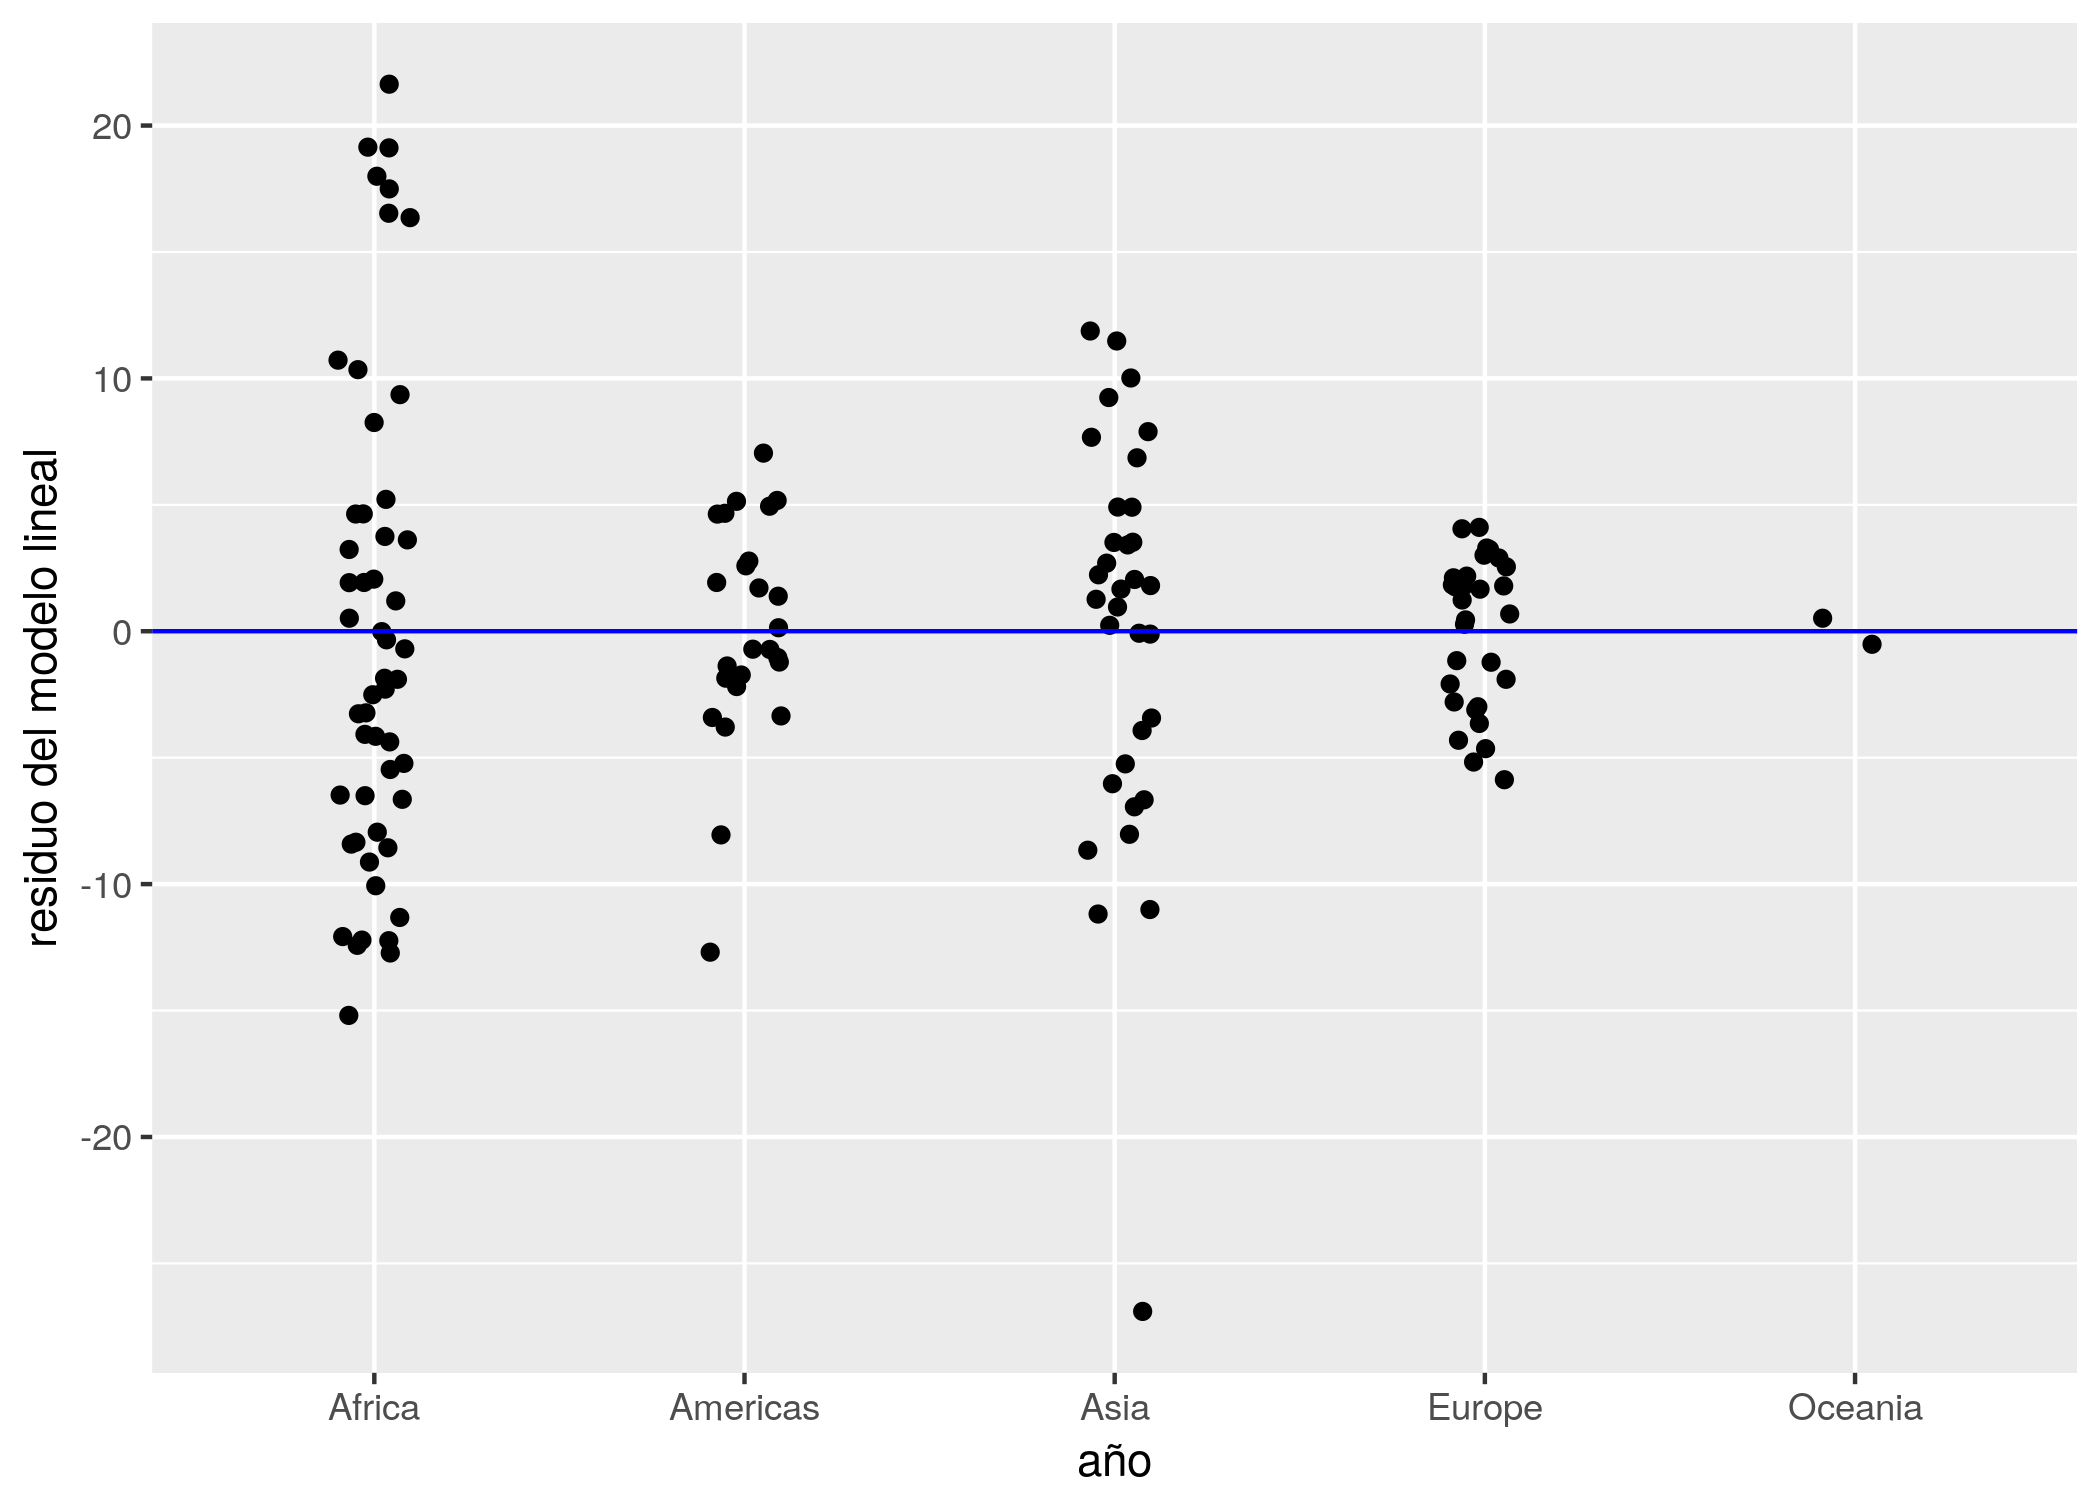
\includegraphics{ciencia_de_datos_para_gente_sociable_files/figure-latex/unnamed-chunk-131-1.pdf}

Notamos que:

\begin{enumerate}
\def\labelenumi{\arabic{enumi}.}
\tightlist
\item
  Los residuos están repartidos en forma pareja entre positivos y
  negativos. Eso indica que su promedio será cercano a cero, lo cual es
  bueno.
\item
  En Asia hay un país cuyo valor observado está muy por debajo del
  esperado por el modelo. Se separa tanto de los demás que debemos
  considerarlo un \emph{outlier}, un valor tan inusual que amerita ser
  revisado.
\end{enumerate}

Con la magia de los verbos de transformación que sabemos, aislemos a los
países en Asia con menor expectativa de vida para encontrar identificar
al \emph{outlier}.

\begin{Shaded}
\begin{Highlighting}[]
\NormalTok{data_mundial_}\DecValTok{2007} \OperatorTok\StringTok{ }
\StringTok{    }\KeywordTok{filter}\NormalTok{(continente }\OperatorTok{==}\StringTok{ "Asia"}\NormalTok{) }\OperatorTok\StringTok{ }
\StringTok{    }\KeywordTok{arrange}\NormalTok{(expVida) }\OperatorTok\StringTok{ }
\StringTok{    }\KeywordTok{head}\NormalTok{()}
\end{Highlighting}
\end{Shaded}

\begin{verbatim}
##          pais continente  año expVida     pobl    PBI_PC residuo_ml
## 1 Afghanistan       Asia 2007  43.828 31889923  974.5803 -26.900485
## 2        Iraq       Asia 2007  59.545 27499638 4471.0619 -11.183485
## 3    Cambodia       Asia 2007  59.723 14131858 1713.7787 -11.005485
## 4     Myanmar       Asia 2007  62.069 47761980  944.0000  -8.659485
## 5 Yemen, Rep.       Asia 2007  62.698 22211743 2280.7699  -8.030485
## 6       Nepal       Asia 2007  63.785 28901790 1091.3598  -6.943485
\end{verbatim}

Se trata de Afganistán. Como explicación, uno piensa de inmediato en las
largas guerras libradas en ese territorio, y en particular la invasión
por parte de los Estados Unidos en 2001 -¡otra vez ese año!-. Podemos
verificarlo con un gráfico que muestre la evolución de la expectativa de
vida según los años.

\begin{Shaded}
\begin{Highlighting}[]
\NormalTok{data_afganistan <-}\StringTok{ }\NormalTok{data_mundial }\OperatorTok\StringTok{ }\KeywordTok{filter}\NormalTok{(pais }\OperatorTok{==}\StringTok{ "Afghanistan"}\NormalTok{)}

\KeywordTok{ggplot}\NormalTok{(data_afganistan) }\OperatorTok{+}\StringTok{ }
\StringTok{    }\KeywordTok{geom_line}\NormalTok{(}\KeywordTok{aes}\NormalTok{(}\DataTypeTok{x =}\NormalTok{ año, }\DataTypeTok{y =}\NormalTok{ expVida)) }\OperatorTok{+}
\StringTok{    }\KeywordTok{labs}\NormalTok{(}\DataTypeTok{title =} \StringTok{"Expectativa de vida en Afganistán"}\NormalTok{,}
         \DataTypeTok{y =} \StringTok{"expectativa de vida"}\NormalTok{)}
\end{Highlighting}
\end{Shaded}

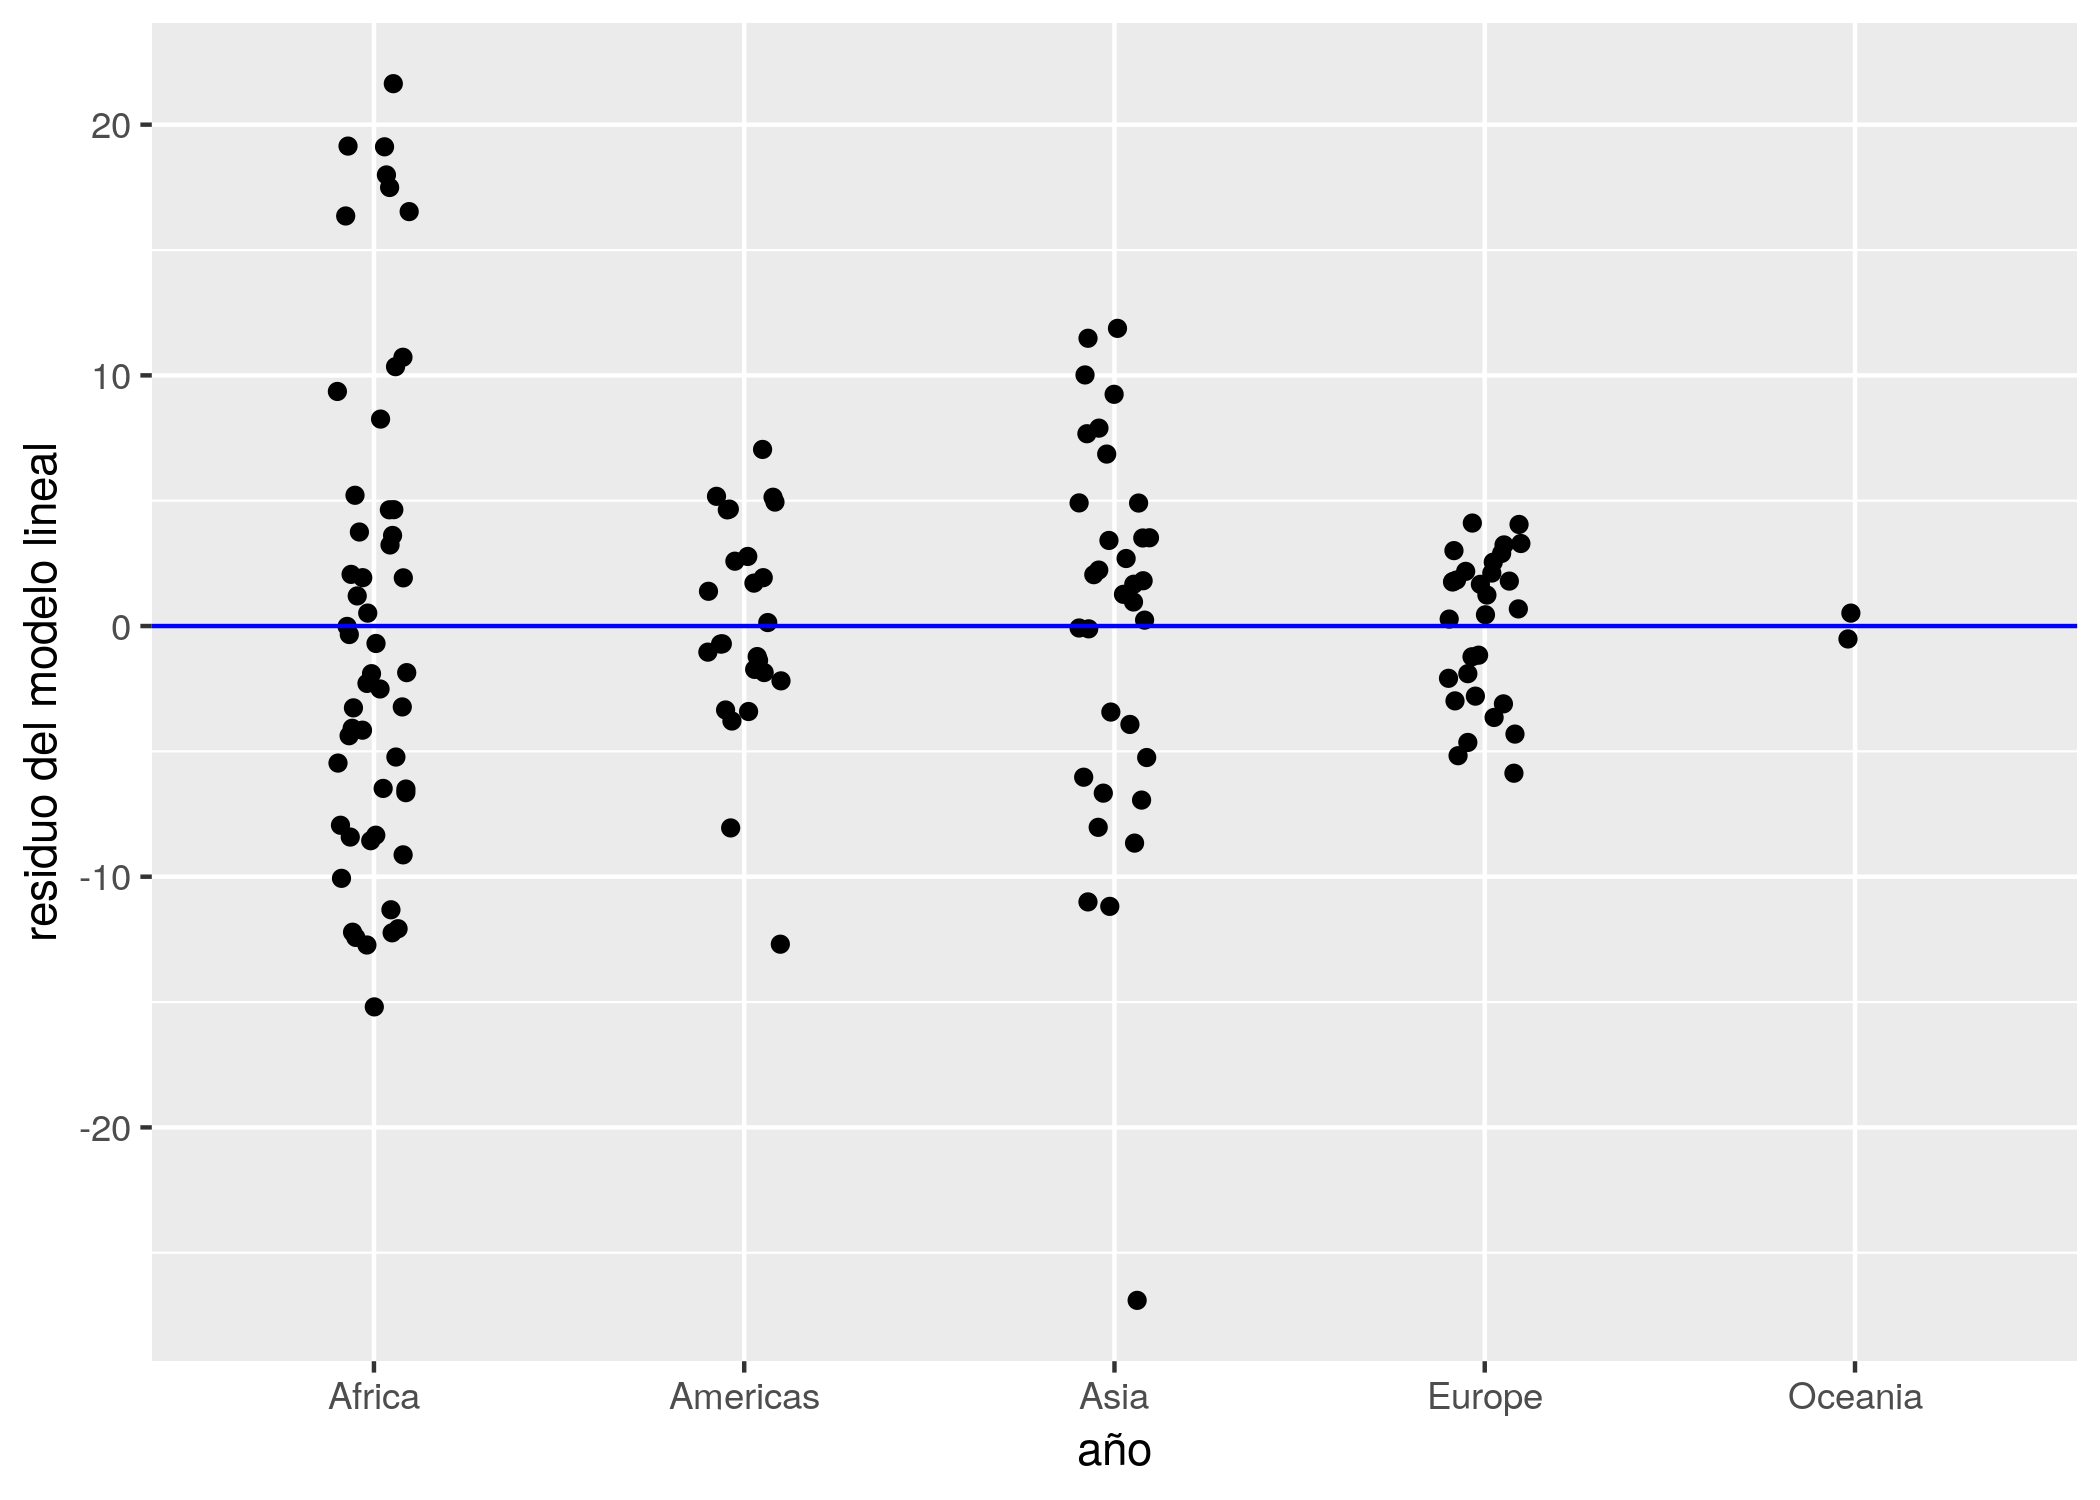
\includegraphics{ciencia_de_datos_para_gente_sociable_files/figure-latex/unnamed-chunk-133-1.pdf}

Vaya sopresa. A pesar de ser en extremo baja comparada con el resto de
Asia, la expectativa de vida en Afganistán en el 2007 es la más alta de
la historia, y no sólo eso: ha aumentado con rapidez \emph{después} del
año de la invasión. ¿A qué podemos atribuir entonces la bajísima
expectativa de vida? Teniendo en cuenta que el país ha sufrido
conflictos bélicos en forma continua desde fines de los '70, podría
tratarse de una tragedia histórica: los años que faltan son los que el
país habría alcanzado si las guerras no hubieran alterado su ritmo de
progreso.

Dependiendo del esfuerzo que requiera determinar la causa de un
\emph{outlier}, una alternativa razonable es dejarlo de lado. Es un poco
cruel, pero realista: cuando tenemos cientos, miles o millones de
observaciones, hacer una ``poda'' de los valores extremos que nuestros
modelos no pueden explicar termina siendo la opción más razonable.
Dedicar recursos limitados a la caza de una explicación o a complejizar
el modelo agregando variables hasta lograr predecir los \emph{outliers}
no tiene sentido cuando se trata de casos aislados y fortuitos. Por otra
parte, eliminarlos antes de tiempo podría hacernos ignorar los casos más
interesantes de un dataset, los que más información podrían revelar.
Existen tratados completos dedicados a la cuestión de como manejar los
\emph{outliers}, pero el conocimiento de dominio es la principal
herramienta para decidir que hacer ante casos inusuales\ldots{} como
siempre.

\section{Regresión con múltiples
variables}\label{regresion-con-multiples-variables}

Hasta aquí hemos usado la regresión lineal para hacer explícita la
relación entre una variable \emph{resultante} \(y\) y una única variable
\emph{predictiva} o \emph{explicativa} \(x\). En algunos de nuestros
resultados pudimos intuir que el agregado de alguna variable explicativa
adicional podría mejorar nuestras predicciones. De eso se trata la
regresión lineal múltiple: incorporar una cantidad arbitraria de
variables al modelo, buscando representar las múltiples dinámicas que
inciden en el fenómeno estudiado.

Una buena noticia es que, en general, agregar variables a nuestro modelo
estadístico no requiere mucho esfuerzo adicional. En la época en que los
cálculos matemáticos debían hacerse sin la ayuda de una computadora,
sumar variables sin ton ni son debía tener poca gracia, debido a la
creciente cantidad de cálculos a resolver. Para nosotros que dejamos la
tarea en manos de software especializado, el problema es el opuesto. Es
tan fácil sumar variables al modelo, que debemos evitar la tentación de
arrojar todo dentro de la fórmula de regresión líneal y decidir luego
que parece importante y que no.

Pasemos a la práctica. Vamos a modelar la expectativa como resultante de
la población y del PBI per cápita de los países, usando los datos más
reciente (tomados en 2007). La única difrerencia respecto a una
regresión lineal simple es que usamos \texttt{+} para agregar variables
en la fórmula de \texttt{lm()}

\begin{Shaded}
\begin{Highlighting}[]
\NormalTok{modelo_exp_multiple <-}\StringTok{ }\KeywordTok{lm}\NormalTok{(expVida }\OperatorTok{~}\StringTok{ }\NormalTok{pobl }\OperatorTok{+}\StringTok{ }\NormalTok{PBI_PC, }\DataTypeTok{data =}\NormalTok{ data_mundial_}\DecValTok{2007}\NormalTok{)}

\NormalTok{modelo_exp_multiple}
\end{Highlighting}
\end{Shaded}

\begin{verbatim}
## 
## Call:
## lm(formula = expVida ~ pobl + PBI_PC, data = data_mundial_2007)
## 
## Coefficients:
##     (Intercept)             pobl           PBI_PC  
## 59.205198140717   0.000000007001   0.000641608517
\end{verbatim}

¿Cómo interpretamos esos resultados? Más o menos de la misma manera que
con la regresión simple. Como antes, tenemos un coeficiente para la
intersección, al que no prestamos mucha atención porque no nos dice nada
de la relación entre las variables. Lo que cambia es que esta vez
tenemos dos variables predictoras en lugar a una, cada una con su
coeficiente. Los coeficientes positivos indican que la relación de la
población con la expectativa de vida es de correlación positiva (cuando
una crece la otra tiende a crecer también), y lo mismo ocurre con el
PBI. La magnitud de los coeficientes es pequeña (minúscula en el caso de
la población), lo cual dificulta ``narrar'' los resultados, pero podemos
hacerlo así:

\begin{itemize}
\tightlist
\item
  Cuando las demás variables se mantienen constantes (es decir, en
  países con PBI similar) el incremento de una unidad de población -un
  habitante- está asociado a un incremento de 0,000000007 años en la
  expectativa de vida del país\ldots{} unas dos décimas de segundo.
\item
  Cuando las demás variables se mantienen constantes (es decir, en
  países con población similar) el incremento de una unidad de PBI -un
  dólar per cápita- está asociado a un incremento de 0,00064 años en la
  expectativa de vida del país\ldots{} un poco más de cinco horas y
  media.
\end{itemize}

Pensemos un poco si los resultados tienen sentido. La correlación
positiva entre PBI y longevidad es de lo más razonable. No nos extraña
que los países de mayores ingresos tiendan a ser aquellos cuyos
habitantes viven más tiempo. La correlación con la población es quizás
inesperada. Si la longevidad se incrementa junto a la cantidad de
habitantes, ¿acaso no deberíamos encontrar a varios de los países más
populosos entre los más longevos?

Veamos el \emph{top ten} de países más poblados:

\begin{Shaded}
\begin{Highlighting}[]
\NormalTok{data_mundial_}\DecValTok{2007} \OperatorTok\StringTok{ }
\StringTok{    }\KeywordTok{arrange}\NormalTok{(}\KeywordTok{desc}\NormalTok{(expVida)) }\OperatorTok\StringTok{ }
\StringTok{    }\KeywordTok{head}\NormalTok{(}\DataTypeTok{n =} \DecValTok{10}\NormalTok{)}
\end{Highlighting}
\end{Shaded}

\begin{verbatim}
##                pais continente  año expVida      pobl   PBI_PC residuo_ml
## 1             Japan       Asia 2007  82.603 127467972 31656.07   11.87452
## 2  Hong Kong, China       Asia 2007  82.208   6980412 39724.98   11.47952
## 3           Iceland     Europe 2007  81.757    301931 36180.79    4.10840
## 4       Switzerland     Europe 2007  81.701   7554661 37506.42    4.05240
## 5         Australia    Oceania 2007  81.235  20434176 34435.37    0.51550
## 6             Spain     Europe 2007  80.941  40448191 28821.06    3.29240
## 7            Sweden     Europe 2007  80.884   9031088 33859.75    3.23540
## 8            Israel       Asia 2007  80.745   6426679 25523.28   10.01652
## 9            France     Europe 2007  80.657  61083916 30470.02    3.00840
## 10           Canada   Americas 2007  80.653  33390141 36319.24    7.04488
\end{verbatim}

y el de países con mayor expectativa de vida:

\begin{Shaded}
\begin{Highlighting}[]
\NormalTok{data_mundial_}\DecValTok{2007} \OperatorTok\StringTok{ }
\StringTok{    }\KeywordTok{arrange}\NormalTok{(}\KeywordTok{desc}\NormalTok{(pobl)) }\OperatorTok\StringTok{ }
\StringTok{    }\KeywordTok{head}\NormalTok{(}\DataTypeTok{n =} \DecValTok{10}\NormalTok{)}
\end{Highlighting}
\end{Shaded}

\begin{verbatim}
##             pais continente  año expVida       pobl    PBI_PC  residuo_ml
## 1          China       Asia 2007  72.961 1318683096  4959.115  2.23251515
## 2          India       Asia 2007  64.698 1110396331  2452.210 -6.03048485
## 3  United States   Americas 2007  78.242  301139947 42951.653  4.63388000
## 4      Indonesia       Asia 2007  70.650  223547000  3540.652 -0.07848485
## 5         Brazil   Americas 2007  72.390  190010647  9065.801 -1.21812000
## 6       Pakistan       Asia 2007  65.483  169270617  2605.948 -5.24548485
## 7     Bangladesh       Asia 2007  64.062  150448339  1391.254 -6.66648485
## 8        Nigeria     Africa 2007  46.859  135031164  2013.977 -7.94703846
## 9          Japan       Asia 2007  82.603  127467972 31656.068 11.87451515
## 10        Mexico   Americas 2007  76.195  108700891 11977.575  2.58688000
\end{verbatim}

El único país presente en ambas listas es Japón. Ni nuestro conocimiento
del mundo, ni los datos parecen apoyar la noción de que población y
longevidad van juntos. Ya hemos usado \texttt{cor()} para obtener una
medida de la intensidad de la correlación entre dos variables. Veamos
que pasa con longevidad vs.~población:

\begin{Shaded}
\begin{Highlighting}[]
\KeywordTok{cor}\NormalTok{(data_mundial_}\DecValTok{2007}\OperatorTok{$}\NormalTok{expVida, data_mundial_}\DecValTok{2007}\OperatorTok{$}\NormalTok{pobl)}
\end{Highlighting}
\end{Shaded}

\begin{verbatim}
## [1] 0.04755312
\end{verbatim}

Recordemos que la intensidad de una correlación es su valor absoluto,
que toma un máximo de 1, mientras que el signo (positivo o negativo)
indica si la relación entre variables es directa o inversa. Aquí
obtuvimos un valor bien bajo, cercano a cero: la correlación es nula.
Entonces ¿Por qué aparece en nuestro modelo de regresión lineal?

En resumidas cuentas, aparece porque nosotros le pedimos que aparezca.
Es decir, instruimos en forma específica a \texttt{lm()} para que
incorpore a la población en el modelo. El caso es que población no es un
buen predictor de longevidad (la correlación es bajísima), pero si lo
pedimos, lo tenemos: el coeficiente nos indica el valor que minimiza las
discrepancias entre valores observado y valores predichos trazando una
línea recta. Lo que no indica por si solo es el grado en el cual podemos
confiar en esa variable para darnos buenas predicciones o estimados.

Sería muy util que el resultado de \texttt{lm()} indique cuáles
variables son buenas predictoras y cuáles no. Y por suerte, lo hace
cuando lo interrogamos con \texttt{summary()}, la misma función que
hemos estado usando para obtener el resumen de un dataframe. Cuando la
usamos con un objeto de R que contiene un modelo estadístico, lo que
obtenemos son sus detalles:

\begin{Shaded}
\begin{Highlighting}[]
\KeywordTok{summary}\NormalTok{(modelo_exp_multiple)}
\end{Highlighting}
\end{Shaded}

\begin{verbatim}
## 
## Call:
## lm(formula = expVida ~ pobl + PBI_PC, data = data_mundial_2007)
## 
## Residuals:
##     Min      1Q  Median      3Q     Max 
## -22.496  -6.119   1.899   7.018  13.383 
## 
## Coefficients:
##                    Estimate      Std. Error t value            Pr(>|t|)
## (Intercept) 59.205198140717  1.040398672164  56.906 <0.0000000000000002
## pobl         0.000000007001  0.000000005068   1.381               0.169
## PBI_PC       0.000641608517  0.000058176209  11.029 <0.0000000000000002
##                
## (Intercept) ***
## pobl           
## PBI_PC      ***
## ---
## Signif. codes:  0 '***' 0.001 '**' 0.01 '*' 0.05 '.' 0.1 ' ' 1
## 
## Residual standard error: 8.87 on 139 degrees of freedom
## Multiple R-squared:  0.4679, Adjusted R-squared:  0.4602 
## F-statistic: 61.11 on 2 and 139 DF,  p-value: < 0.00000000000000022
\end{verbatim}

El resumen incluye los parámetros que definieron al modelo, los valores
por cuartil de los residuos, y una tabla con variables numéricas. En esa
tabla, bajo la columna \texttt{Estimate} tenemos el ``efecto'' estimado
de cada variable explicativa sobre la dependiente. Es decir, los
coeficientes que ya conocemos. Luego aparecen tres columnas con
atributos estadísticos: \texttt{Std.\ Error}, \texttt{t\ value}, y
\texttt{Pr(\textgreater{}\textbar{}t\textbar{})}. En castellano las
llamaríamos, respectivamente, \emph{error estándar}, \emph{valor t} y
\emph{valor p}. Interpretar estos valores cae fuera de nuestros
objetivos, pero podemos señalar que el más famoso entre ellos es el
\emph{valor p}, porque se usa como medida: si vale menos de 0,5, se
considera que la capacidad de predicción de la variable asociada es
significativa. Para interpretar todo esto de manera sencilla, una vez
más vamos a confiar en R para guiarnos. He aquí la curiosa forma de
determinar si una variable es buena predictora o no: contar estrellitas.
Junto a cada fila aparecen, a veces, de uno a tres asteriscos. Son la
forma de R de decirnos cuales son las variables explicativas que
muestran una relación ``estadísticamente significativa'' con nuestra
variable dependiente. Cuanto más bajo el valor p, más significativa es
la relación y más estrellitas aparecen:

\begin{itemize}
\tightlist
\item
  \texttt{.} o nada: No se encuentra una relación entre esta variable y
  la que queremos predecir.
\item
  \texttt{*}: Es muy probable que esta variable tenga una relación con
  la que queremos predecir. Ya podemos publicar estos resultados en un
  paper científico.
\item
  \texttt{**}: Es muy, pero muy probable que esta variable tenga una
  relación con la que queremos predecir. 99\% seguro.
\item
  \texttt{***}: Juramos que las variables estan relacionadas. Más no se
  puede pedir.
\end{itemize}

Lo de un asterisco/estrella (\texttt{*}) indicando que los resultados ya
alcanzan rigor científico no es broma. El asterisco solitario indica
que, a nivel estadístico, se supera el 95\% de confianza en que la
relación existe en la realidad y no es producto de una casualidad en los
datos. Pasando ese umbral se considera que los datos son
``estadísticamente significativos'', y desde hace muchos años encontrar
un \emph{valor p} menor a 0,5 es la meta dorada de los investigadores
que emplean análisis estadístico. ¿Porqué un 95\% de confianza alcanza?
¿Porqué no relajar el límite a 90\%, o quizás mejor, exigir al menos un
99 o 99,9\% de seguridad? La verdad es que no hay ninguna razón
trascendental. El 95\% de certeza es tan sólo un valor arbitrario que en
algún momento se volvió estándar. Es importante aclara que en los
últimos años ha crecido una reacción de rechazo a esta norma arbitraria,
dentro de la propia comunidad científica. Quienes siguen confiando en
los \emph{valores p} son llamados ``frecuentistas''; los que proponen
cuantificar de otra forma nuestro grado de certeza son llamados
``bayesianos''. Google mediante, quien quiera saber más sobre la
apasionante rivalidad tendrá horas de diversión aseguradas.

En lo que a nosotros respecta, por ahora vamos a aceptar el enfoque
frecuentista, y cuando veamos una estrella diremos que la variable
asociada es un buen predictor. O para ser más precisos, que su relación
con la variable dependiente es estadísticamente significativa.

Volvamos a nuestros modelos. Cuando hicimos regresiones simples no
sabíamos aún de valores p, y no revisamos la significancia de las
variables predictoras. Hagamoslo ahora con el modelo de expectativa de
vida en Argentina vs.~PBI :

\begin{Shaded}
\begin{Highlighting}[]
\KeywordTok{summary}\NormalTok{(modelo_exp)}
\end{Highlighting}
\end{Shaded}

\begin{verbatim}
## 
## Call:
## lm(formula = expVida ~ año, data = data_arg)
## 
## Residuals:
##      Min       1Q   Median       3Q      Max 
## -0.53006 -0.13516 -0.01219  0.14228  0.55202 
## 
## Coefficients:
##                Estimate  Std. Error t value          Pr(>|t|)    
## (Intercept) -389.606345    9.677730  -40.26 0.000000000002140 ***
## año            0.231708    0.004889   47.40 0.000000000000422 ***
## ---
## Signif. codes:  0 '***' 0.001 '**' 0.01 '*' 0.05 '.' 0.1 ' ' 1
## 
## Residual standard error: 0.2923 on 10 degrees of freedom
## Multiple R-squared:  0.9956, Adjusted R-squared:  0.9951 
## F-statistic:  2246 on 1 and 10 DF,  p-value: 0.0000000000004216
\end{verbatim}

Las tres estrellitas, distintión máxima, indican que sin dudas el año
está relacionado con la expectativa de vida. Esto no es una sopresa: la
linea de la regresión lineal se ajusta con tanta precisión a los valores
observados, que no podía ser de otra manera.

Continuando con las regresiones múltiples, intentemos un modelo con tres
variables predictoras. A población y PBI, las que ya teníamos en cuenta,
vamos a agregar una variable categórica: el continente.

\begin{Shaded}
\begin{Highlighting}[]
\NormalTok{modelo_exp_multiple <-}\StringTok{ }\KeywordTok{lm}\NormalTok{(expVida }\OperatorTok{~}\StringTok{ }\NormalTok{pobl }\OperatorTok{+}\StringTok{ }\NormalTok{PBI_PC }\OperatorTok{+}\StringTok{ }\NormalTok{continente, }\DataTypeTok{data =}\NormalTok{ data_mundial_}\DecValTok{2007}\NormalTok{)}

\KeywordTok{summary}\NormalTok{(modelo_exp_multiple)}
\end{Highlighting}
\end{Shaded}

\begin{verbatim}
## 
## Call:
## lm(formula = expVida ~ pobl + PBI_PC + continente, data = data_mundial_2007)
## 
## Residuals:
##      Min       1Q   Median       3Q      Max 
## -22.8199  -2.8905   0.1574   2.9046  20.0585 
## 
## Coefficients:
##                            Estimate       Std. Error t value
## (Intercept)        53.7141900516204  0.9355709763972  57.413
## pobl                0.0000000009586  0.0000000039259   0.244
## PBI_PC              0.0003479123814  0.0000571704015   6.086
## continenteAmericas 16.0313726693021  1.6713252557392   9.592
## continenteAsia     12.5640427449841  1.6209815371922   7.751
## continenteEurope   15.1989177617593  1.9662500363509   7.730
## continenteOceania  16.6222095573924  4.9925674316223   3.329
##                                Pr(>|t|)    
## (Intercept)        < 0.0000000000000002 ***
## pobl                            0.80747    
## PBI_PC                 0.00000001127738 ***
## continenteAmericas < 0.0000000000000002 ***
## continenteAsia         0.00000000000197 ***
## continenteEurope       0.00000000000220 ***
## continenteOceania               0.00112 ** 
## ---
## Signif. codes:  0 '***' 0.001 '**' 0.01 '*' 0.05 '.' 0.1 ' ' 1
## 
## Residual standard error: 6.597 on 135 degrees of freedom
## Multiple R-squared:  0.7141, Adjusted R-squared:  0.7014 
## F-statistic:  56.2 on 6 and 135 DF,  p-value: < 0.00000000000000022
\end{verbatim}

Observamos que la variable categórica es significativa. Con las demas
variables fijas -es decir, en paises de similar PBI y población- el
continente de origen explica en gran medida las diferencias en
expectativa de vida en cada país, y con un efecto estimado enorme - ¡de
12 a 16 años!-. Notemos de todos modos que el coeficiente de la variable
continente había sido mayor en el modelo simple, llegando a casi 26 años
para Oceanía. ¿Porqué es menor ahora? Porque nuestro modelo es más
completo, y tiene en cuenta más variables. Cuando lo único que teníamos
para comparar países era su continente, era era la única variable a la
que atribuir diferencias. Ahora que consideramos mútiples variables para
explicar las diferencias, notamos la parte de la influencia que se lleva
el PBI, reduciendo la del contintente.

\chapter{Información geográfica y
mapas}\label{informacion-geografica-y-mapas}

Hemos llegado al capítulo final, dedicado al análisis y visualización de
información geográfica. Aquí incursionaremos en el el dominio de los
\emph{SIG} (``Sistemas de Información Geográfica'') también conocidos
como \emph{GIS} por sus siglas en inglés.

Hasta hace poco tiempo, labores como la producción de mapas y el
análisis espacial estaban reservadas para especialistas, debido a la
complejidad de las tareas y al alto costo de producción y adquisición de
datos geográficos. Pero durante las dos últimas décadas la tecnología
digital cambió el panorama. Una dramática caída en el costo asociado a
adquirir y procesar información geográfica (pensemos en satélites y
computadoras multiplicándose y bajando de precio) dio paso al mapa
digital como herramienta universal. El consumo de sofisticados mapas y
otros productos geográficos se volvió masivo y cotidiano, con Google
Maps como el exponente más conocido. Apenas había pasado la novedad de
disponer de mapas en alta resolución de todo el mundo accesibles al
instante desde nuestros escritorios, cuando la llegada de los
\emph{smartphones} popularizó el acceso en cualquier momento y lugar.

El mismo proceso que nos convirtió a todos en consumidores constantes de
información geográfica también nos da la oportunidad de ser los
productores. Sin dudas, hacer mapas se ha vuelto más fácil que nunca
antes. Existen cada vez más repositorios con información
georreferenciada de acceso publico -datasets que incluyen información
precisa sobre su ubicación geográfica. Al mismo tiempo, maduran y se
hacen más fáciles de usar las herramientas para análisis y visualización
espacial.

En los procesos sociales, el ``dónde'' suele ser un aspecto clave,
central para quienes estudiamos, por ejemplo, las ciudades o las
dinámicas de la política, siempre tan arraigadas a lo territorial. Esto
vuelve al mapa una de las herramientas de visualización más importantes
que podemos emplear.

En R contamos con varios paquete de funciones que permiten manipular
información espacial con facilidad. A continuación vamos a aprender a
combinarlos con las herramientas que ya hemos aprendido, para hacer
análisis geográfico y crear nuestros propios mapas.

\section{Los datos georreferenciados}\label{los-datos-georreferenciados}

El atributo que distingue a los datos georreferenciados, lo que los hace
merecer ese nombre, es que representan ubicaciones exactas sobre la
superficie de la Tierra. Representar en forma precisa una posición sobre
la superficie terrestre es un todo un reto. Para empezar, la Tierra
tiene una forma irregular. A pesar de cómo solemos imaginarla y
dibujarla, no es una esfera perfecta sino que está ``achatada'' en los
polos, dificultando la matemática necesaria para comparar posiciones y
medir distancias. Luego, está el problema de cómo mostrar sobre papel
impreso, o en una pantalla digital, -superficies planas- rasgos
geográficos que pertenecen a una superficie tridimensional esférica. La
solución a estos problemas toma la forma de sistemas de coordenadas de
referencia (\emph{CRS} por sus siglas en inglés), y de proyecciones
cartográficas.

Los CRS son un sistema de números que definen ubicaciones sobre la
superficie de la Tierra; funcionan como direcciones. El tipo de CRS más
conocido es el que usa latitud y longitud, para definir posiciones en
los ejes norte-sur y este-oeste.

Las proyecciones cartográficas son instrucciones para traducir a un
plano la disposición de puntos ubicados en la esfera terrestre. Algo así
como las instrucciones para dibujar en dos dimensiones las disposición
de fronteras, accidentes geográficos, calles o cualquier otro objeto que
se extiende sobre la superficie curva del planeta. Como en toda
traducción, hay algo que se pierde en el proceso. Todo los mapas
``mienten'', en el sentido en que presentan una versión distorsionada de
la superficie de terrestre. Esto es inevitable; no existe forma de pasar
de la esfera al plano sin distorsionar la forma, la superficie, la
distancia o la dirección de los rasgo geográficos. Existen muchísimas
proyecciones distintas, cada una pensada para minimizar alguno de los
tipos de distorsión, o para encontrar una solución de compromiso que los
balancee.

\begin{figure}
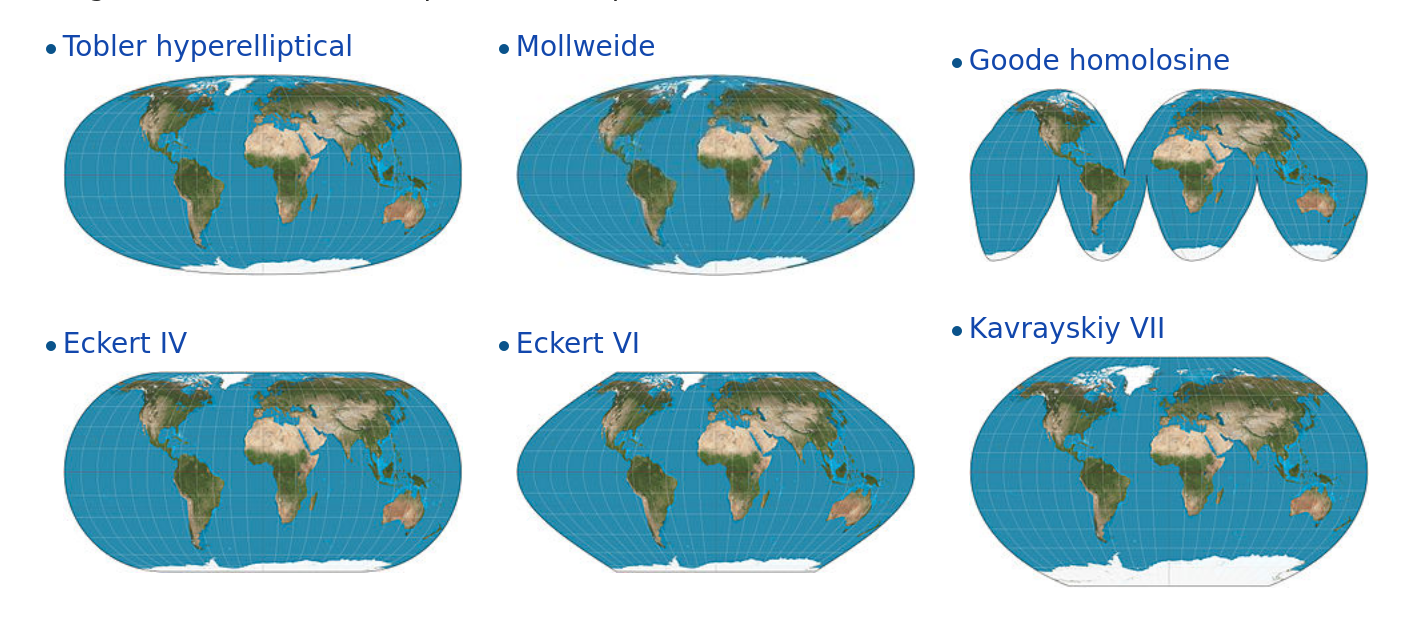
\includegraphics[width=9.49in]{imagenes/proyecciones} \caption{Distintos sistemas de proyección cartográfica (cortesía Daniel R. Strebe 2011)}\label{fig:unnamed-chunk-141}
\end{figure}

La proyección más famosa es la Mercator, diseñada para asistir la
navegación marítima y en uso desde el siglo XVI. Su fuerte es que no
distorsiona las direcciones, por lo que permite fijar el rumbo de
navegación consultando el mapa. Su principal problema es que produce una
distorsión notable en las áreas cercanas a los polos: Groenlandia
aparenta el mismo tamaño que toda África, cuando en realidad tiene sólo
un quinceavo de su superficie. Por esa razón perdió la proyección
popularidad en el siglo XX cuando comenzaron a preferirse proyecciones
que respetan las áreas, como las de la Figura 6.1. Sin embargo, en el
siglo XXI la proyección Mercator recuperó protagonismo. Google la eligió
para sus mapas en línea, y por razones de compatibilidad otros
proveedores de mapas digitales la adoptaron también. Así, y para
inconsolable irritación de los geógrafos, Mercator se convirtió en el
estándar de facto para aplicaciones geográficas en la web.

\begin{figure}
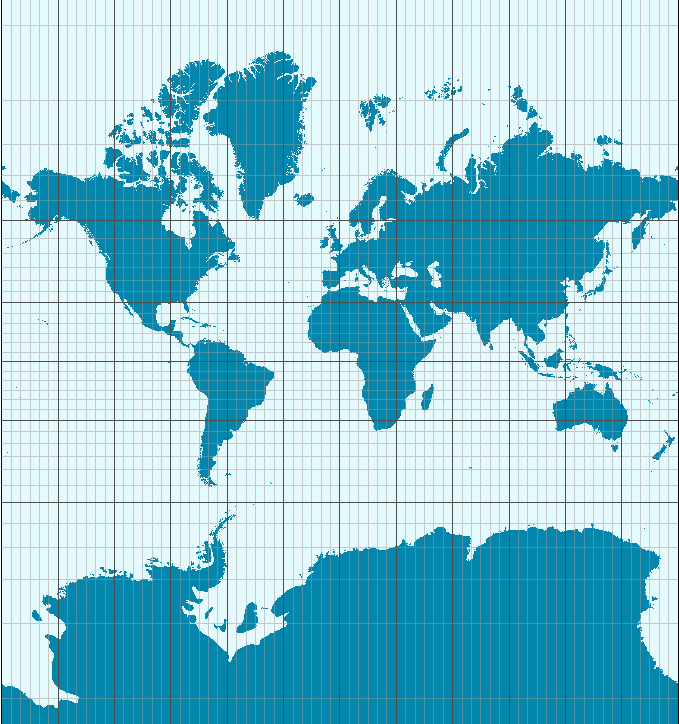
\includegraphics[width=4.53in]{imagenes/Mercator-proj} \caption{La inescapable proyección Mercator (cortesía Jecowa)}\label{fig:unnamed-chunk-142}
\end{figure}

En la práctica, si trabajamos en forma frecuente con archivos
georreferenciados vamos a sufrir tarde o temprano de problemas de
coordenadas o proyección. El más común de ellos: tener una fuentes de
datos geográficos que no podemos comparar con otras, porque desconocemos
el sistema de coordenadas que se usó para crearla; es decir, no podemos
saber a que posición sobre el planeta corresponde cada observación en
los datos.

\section{Formatos de archivo}\label{formatos-de-archivo}

Otro problema asociado a trabajar con datos geográficos es el de los
formatos de archivo. El formato más común es el denominado
``shapefile'', inventado por la empresa ESRI (los creadores del software
ArcGIS). Es un formato incómodo porque guarda la información en varios
archivos distintos, que suelen ser combinados en un archivo .zip para su
distribución. Un inconveniente aún mayor es que los nombres de las
variables en un shapefile deben tener 10 caracteres o menos, lo que
facilita el uso de abreviaturas ininteligibles. A pesar de éstos y otros
detrimentos, el formato es tan común que se ha vuelto sinónimo de
archivo con información geográfica, y resiste a pesar de los esfuerzos
por reemplazarlo con alternativas más modernas. Una de ellas es
``GeoJSON'', un estándar abierto que corrige los dos inconvenientes
mencionados antes. Para nuestros ejercicios usaremos datos geográficos
en esta último formato.

\section{Explorando un archivo con información
geográfica}\label{explorando-un-archivo-con-informacion-geografica}

Como hemos hecho antes, practicaremos con datos tomados del portal de
datos abiertos de la Ciudad de Buenos Aires. En esta ocasión se trata de
los radios censales de la ciudad. Los radios censales son particiones de
la superficie de la ciudad que contienen una cantidad similar de
hogares. Fueron definidos por el Instituto Nacional de Estadística y
Censos (INDEC) para facilitar la labor durante la jornada del Censo
Nacional de Población que se realiza cada diez años. La idea es asignar
a cada censista un radio censal, estimando que puede recorrer todos los
hogares incluidos durante el día. Los radios censales son la unidad de
análisis espacial por excelencia, debido a que combinan alta
granularidad con abundante información asociada de acceso público,
producida como resultado del Censo.

A trabajar entonces. Si no lo hicimos aún, carguemos las librerías
\texttt{sf} y \texttt{tidyverse}

\begin{Shaded}
\begin{Highlighting}[]
\KeywordTok{library}\NormalTok{(sf)}
\KeywordTok{library}\NormalTok{(tidyverse)}
\end{Highlighting}
\end{Shaded}

Y leemos los datos directo desde internet:

\begin{Shaded}
\begin{Highlighting}[]
\NormalTok{radios <-}\StringTok{ }\KeywordTok{st_read}\NormalTok{(}\StringTok{"https://bitsandbricks.github.io/data/CABA_rc.geojson"}\NormalTok{)}
\end{Highlighting}
\end{Shaded}

\begin{verbatim}
## Reading layer `CABA_rc' from data source `https://bitsandbricks.github.io/data/CABA_rc.geojson' using driver `GeoJSON'
## Simple feature collection with 3554 features and 8 fields
## geometry type:  MULTIPOLYGON
## dimension:      XY
## bbox:           xmin: -58.53092 ymin: -34.70574 xmax: -58.33455 ymax: -34.528
## epsg (SRID):    4326
## proj4string:    +proj=longlat +datum=WGS84 +no_defs
\end{verbatim}

Dediquemos un momento para describir la información que apareció al leer
el archivo.

\begin{itemize}
\tightlist
\item
  \texttt{Simple\ feature\ collection\ with\ 3554\ features\ and\ 8\ fields}:
  Cargamos una colección de ``simple features'' (entidades geométricas
  en la jerga de la cartografía digital), compuesta por 3554 rasgos y 8
  campos, que se traduce como 3554 observaciones/filas con 8
  variables/columnas.
\item
  \texttt{geometry\ type:\ \ MULTIPOLYGON}: los archivos con información
  geográfica contienen colecciones de puntos, de líneas, o de polígonos.
  En éste caso son polígonos; tiene sentido para la información que
  esperamos, que es la de la superficie de Buenos Aires dividida en sus
  radios censales.
\item
  \texttt{dimension:\ \ \ \ \ \ XY}: la información es ``plana'', en dos
  dimensiones X e Y. No incluye información de alturas, que estaría en
  la dimensión Z. Es lo típico, rara vez trabajaremos con archivos
  tridimensionales.
\item
  \texttt{bbox:\ \ \ \ \ \ \ \ \ \ \ xmin:\ -58.53092\ ymin:\ -34.70574\ xmax:\ -58.33455\ ymax:\ -34.528}:
  nos da cuatro valores que forman una ``caja'' (\emph{bounding box}),
  el rectángulo que contiene todos los datos. Estos valores son la
  latitud mínima, la longitud mínima, la latitud máxima y la longitud
  máxima del conjunto de datos. Sólo es útil cuando tenemos mucha
  práctica y ya reconocemos lugares por sus coordenadas.
\item
  \texttt{epsg\ (SRID):\ \ \ \ 4326} y
  \texttt{proj4string:\ \ \ \ +proj=longlat\ +datum=WGS84\ +no\_defs}
  significan lo mismo, que nuestros datos usan el sistema de coordenadas
  WGS84, también conocido por su código EPSG 4326 . Es el mismo que usan
  los sistemas GPS, Google Maps, y las aplicaciones de internet en
  general. Es importante prestar atención al sistemas de coordenadas, o
  CRS, ya que para comparar datos geográficos de distintas fuentes todas
  deben usar el mismo.
\end{itemize}

Como con cualquier otro dataset, comenzamos nuestra exploración pidiendo
su resumen:

\begin{Shaded}
\begin{Highlighting}[]
\KeywordTok{summary}\NormalTok{(radios)}
\end{Highlighting}
\end{Shaded}

\begin{verbatim}
##     RADIO_ID          BARRIO         COMUNA       POBLACION     
##  1_1_1  :   1   PALERMO  : 295   1      : 329   Min.   :   0.0  
##  1_10_1 :   1   CABALLITO: 215   13     : 305   1st Qu.: 646.2  
##  1_10_10:   1   RECOLETA : 198   14     : 295   Median : 786.0  
##  1_10_11:   1   BALVANERA: 191   3      : 254   Mean   : 813.2  
##  1_10_12:   1   FLORES   : 183   4      : 252   3rd Qu.: 928.0  
##  1_10_13:   1   BELGRANO : 170   7      : 250   Max.   :3945.0  
##  (Other):3548   (Other)  :2302   (Other):1869                   
##    VIVIENDAS         HOGARES        HOGARES_NBI        AREA_KM2       
##  Min.   :   0.0   Min.   :   0.0   Min.   :  0.00   Min.   :0.004468  
##  1st Qu.: 311.2   1st Qu.: 259.0   1st Qu.:  2.00   1st Qu.:0.018626  
##  Median : 377.0   Median : 310.0   Median :  6.00   Median :0.035548  
##  Mean   : 401.4   Mean   : 323.6   Mean   : 19.35   Mean   :0.057350  
##  3rd Qu.: 462.0   3rd Qu.: 371.0   3rd Qu.: 23.00   3rd Qu.:0.062847  
##  Max.   :1405.0   Max.   :1093.0   Max.   :403.00   Max.   :3.804422  
##                                                                       
##           geometry   
##  MULTIPOLYGON :3554  
##  epsg:4326    :   0  
##  +proj=long...:   0  
##                      
##                      
##                      
## 
\end{verbatim}

Podemos sacar en limpio varias cosas. RADIO\_ID, por su nombre, debe ser
el código que identifica cada radio censal. Tenemos columnas
representando barrio y comuna de cada radio. Tenemos una columna para la
población, y vemos que así como algún radio está deshabitado, el más
poblado alcanza los 3945 habitantes. En cantidad de viviendas, el máximo
es de 1405, y el de hogares 1093: eso significa que existe al menos un
radio censal donde hay viviendas desocupadas; tomamos nota para
revisarlo luego. ``HOGARES\_NBI'' representa la cantidad de hogares
donde se registró que al menos una de las necesidades básicas no estaba
satisfecha, con mínimo de 0 por radio, y máximo nada menos que de 403.
También tenemos una columna con el área en km\^{}2, que muestra que en
general los radios censales abarcan alrededor de medio kilómetro
cuadrado, pero existe alguno que es casi 8 veces mayor al promedio. Por
último queda la columna \texttt{geometry}, que contiene una serie de
puntos que permiten trazar la silueta de cada radio (sus polígonos).
Nosotros no vamos a prestarle atención, pero para R es fundamental, ya
que le permite proyectar mapas y hacer cálculos geométricos cuando se lo
pidamos.

\section{Visualizando información
geográfica}\label{visualizando-informacion-geografica}

La visualización de información geográfica por excelencia es el mapa,
¡por supuesto!

Nuestro aliado \texttt{ggplot()} se encarga de ello.

\begin{Shaded}
\begin{Highlighting}[]
\KeywordTok{ggplot}\NormalTok{() }\OperatorTok{+}\StringTok{ }\KeywordTok{geom_sf}\NormalTok{(}\DataTypeTok{data =}\NormalTok{ radios)}
\end{Highlighting}
\end{Shaded}

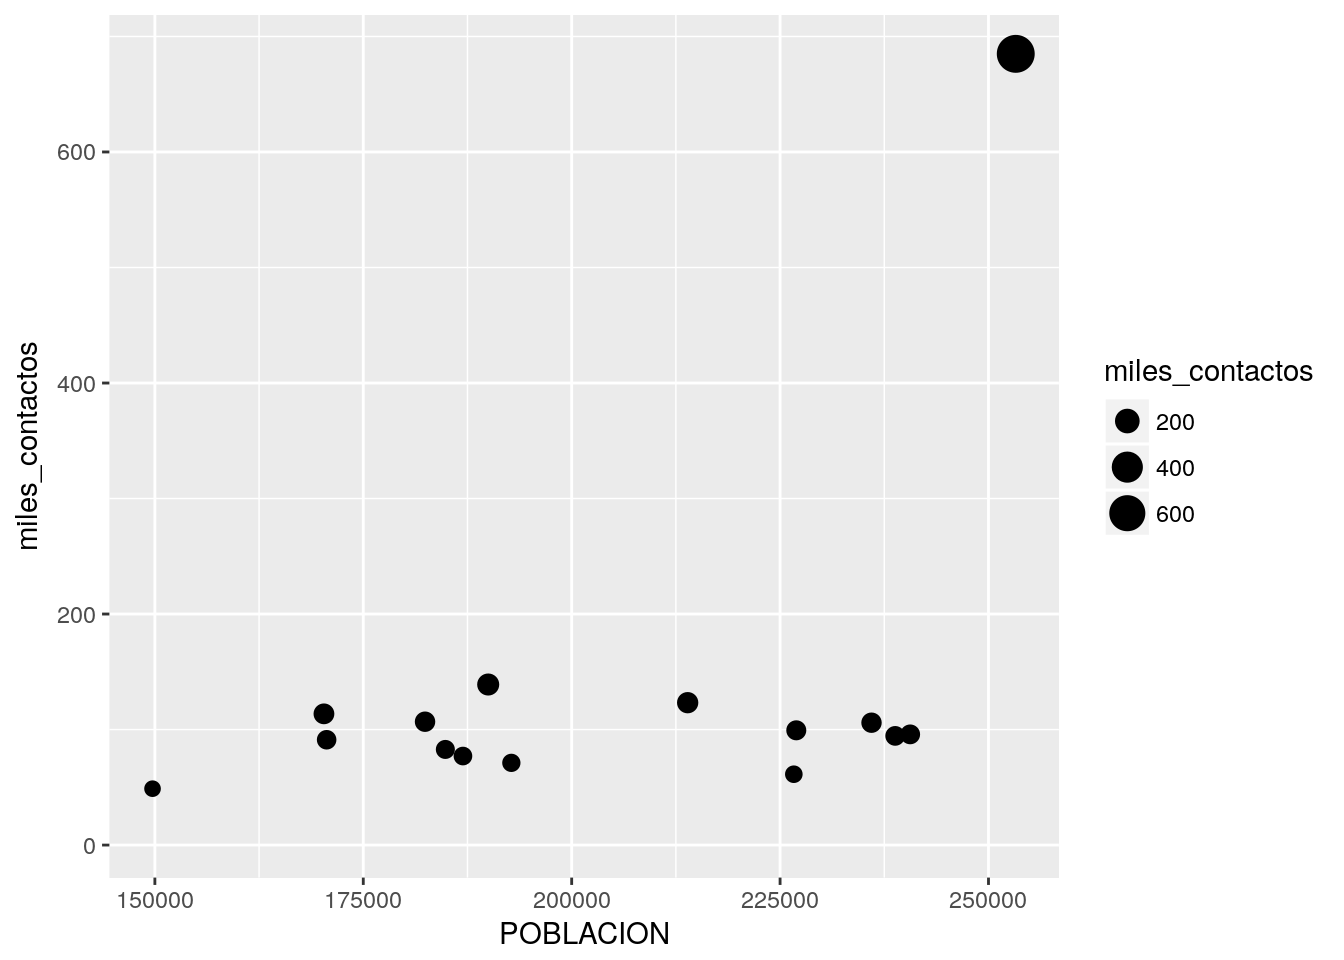
\includegraphics{ciencia_de_datos_para_gente_sociable_files/figure-latex/unnamed-chunk-146-1.pdf}

Ademas de encontrarnos con la reconocible silueta de la ciudad,
comprobamos lo que el resumen de la data había sugerido: la mayoría de
los radios censales tiene un tamaño similar, pero existe un puñado que
es considerablemente más extenso que el promedio. Los ``mega radios''
seguramente corresponden a zonas poco habitadas, por lo que se asume que
un censista puede terminar de encuestar a todos los residentes en un
día.

Podemos analizar eso mismo: ¿cuántas viviendas hay por radio?

\begin{Shaded}
\begin{Highlighting}[]
\KeywordTok{ggplot}\NormalTok{() }\OperatorTok{+}\StringTok{ }\KeywordTok{geom_sf}\NormalTok{(}\DataTypeTok{data =}\NormalTok{ radios, }\KeywordTok{aes}\NormalTok{(}\DataTypeTok{fill =}\NormalTok{ VIVIENDAS)) }
\end{Highlighting}
\end{Shaded}

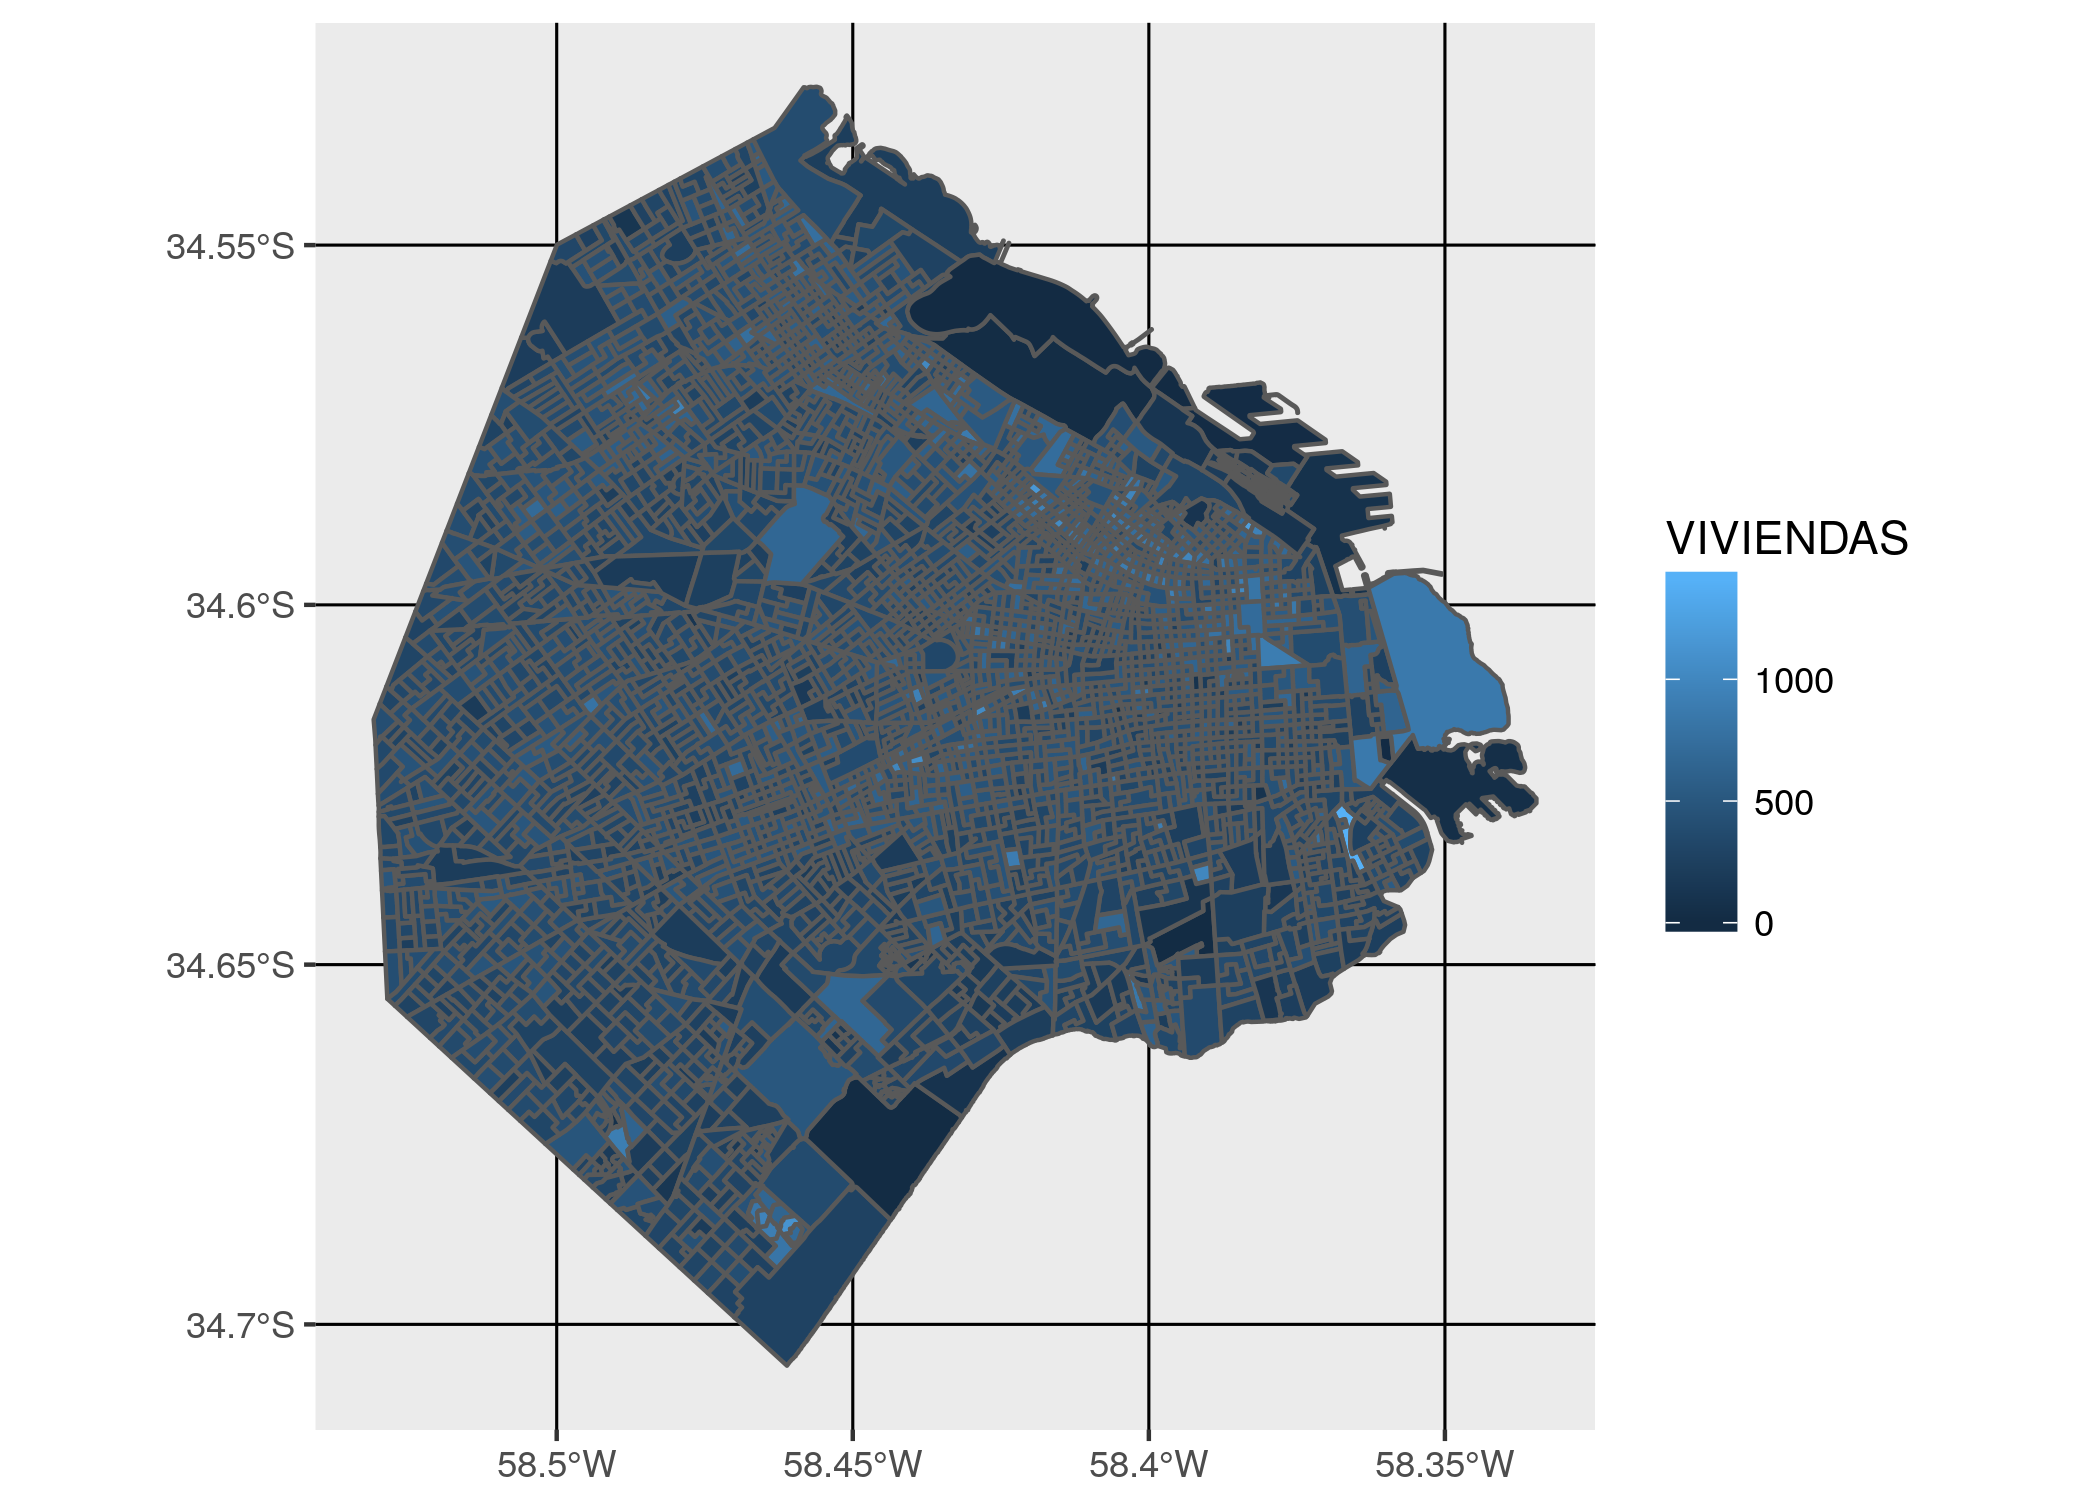
\includegraphics{ciencia_de_datos_para_gente_sociable_files/figure-latex/unnamed-chunk-147-1.pdf}

EL grosor de la línea que traza las fronteras entre radios hace difícil
determinar el color de relleno. Esto suele pasar cuando se grafica
información geográfica intrincada como la de los radios censales. Una
solución es definir el color de la línea como \texttt{NA}, que para
\texttt{ggplot} significa ``ninguno''. Lo hacemos así:

\begin{Shaded}
\begin{Highlighting}[]
\KeywordTok{ggplot}\NormalTok{() }\OperatorTok{+}\StringTok{ }\KeywordTok{geom_sf}\NormalTok{(}\DataTypeTok{data =}\NormalTok{ radios, }\KeywordTok{aes}\NormalTok{(}\DataTypeTok{fill =}\NormalTok{ POBLACION), }\DataTypeTok{color =} \OtherTok{NA}\NormalTok{)}
\end{Highlighting}
\end{Shaded}

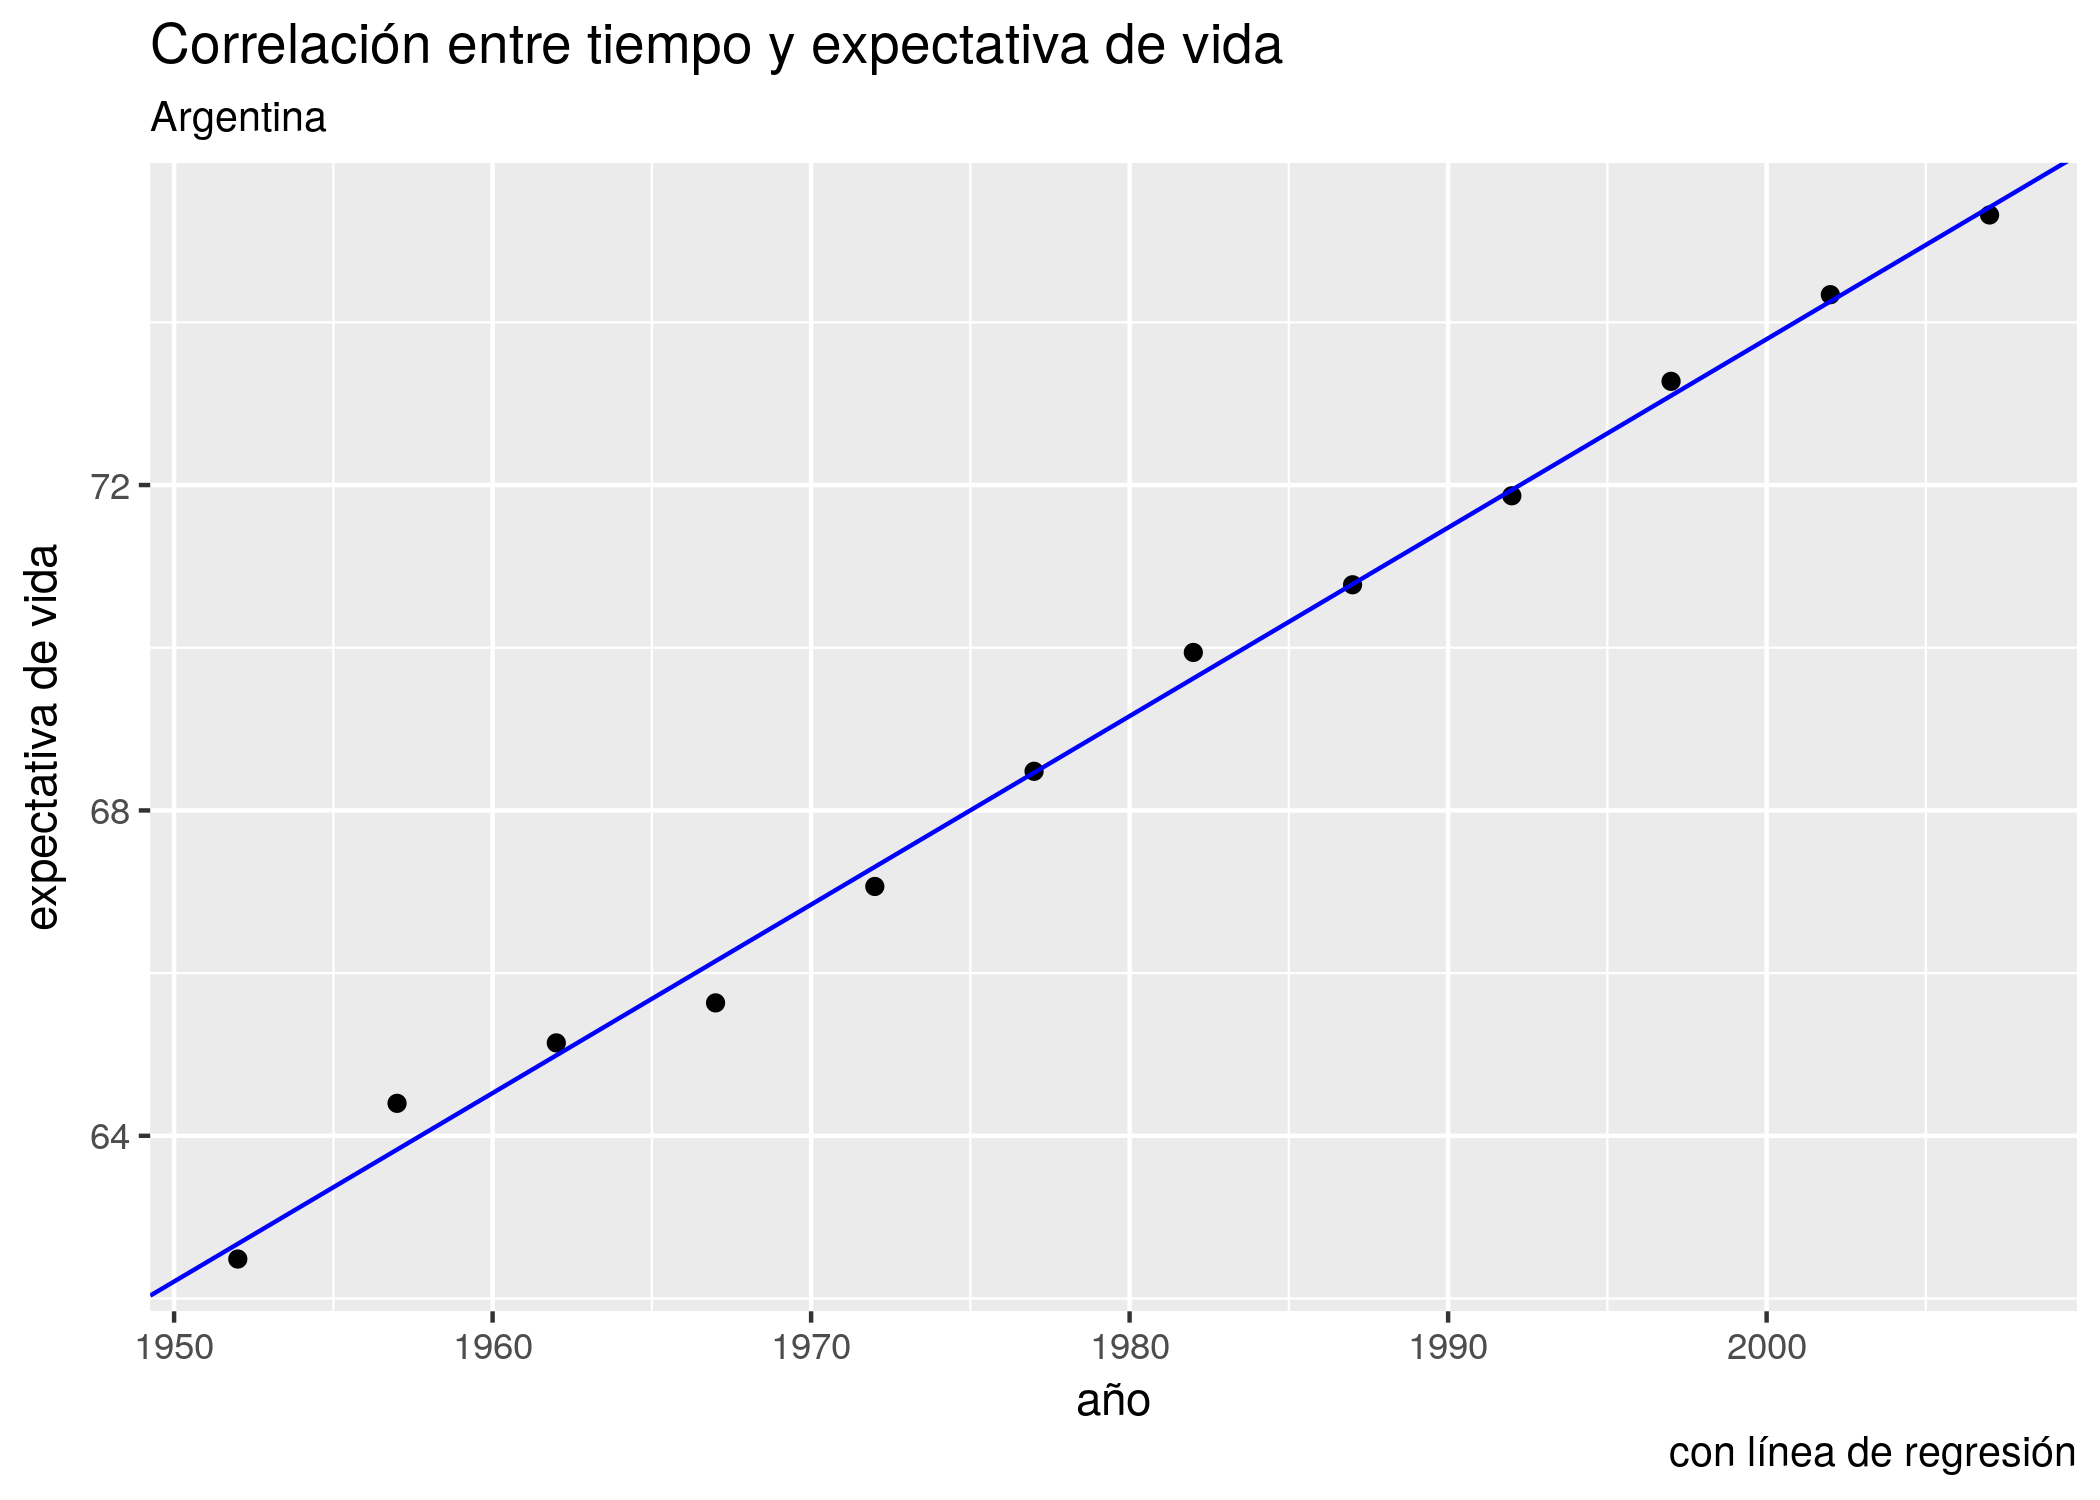
\includegraphics{ciencia_de_datos_para_gente_sociable_files/figure-latex/unnamed-chunk-148-1.pdf}

Así esta mejor. Nótese que definimos el color por fuera de
\texttt{aes()}. Cuando queremos asignar un valor fijo a alguno de los
atributos estéticos (y no dependiente de una variable) siempre va fuera
de la función \texttt{aes()}.

En cuanto al gráfico, observamos que los radios censales más grandes
tienden a ser poco poblados, con algunas excepciones, en particular el
gran radio censal al oeste. ¿A qué barrio corresponde?

\begin{Shaded}
\begin{Highlighting}[]
\KeywordTok{ggplot}\NormalTok{() }\OperatorTok{+}\StringTok{ }\KeywordTok{geom_sf}\NormalTok{(}\DataTypeTok{data =}\NormalTok{ radios, }\KeywordTok{aes}\NormalTok{(}\DataTypeTok{fill =}\NormalTok{ BARRIO), }\DataTypeTok{color =} \OtherTok{NA}\NormalTok{)}
\end{Highlighting}
\end{Shaded}

\includegraphics{ciencia_de_datos_para_gente_sociable_files/figure-latex/unnamed-chunk-149-1.pdf}

Hemos logrado otro de nuestros gráficos ilegibles, intentando mostrar
demasiadas variables categóricas a la vez. Una forma de resolver el
dilema es filtrando los datos para aislar los casos de interés. Del menú
de visualizaciones que aprendimos en el capítulo 2, podemos elegir el
histograma para mostrar la distribución de tamaños de nuestros radios
censales.

\begin{Shaded}
\begin{Highlighting}[]
\KeywordTok{ggplot}\NormalTok{() }\OperatorTok{+}\StringTok{ }\KeywordTok{geom_histogram}\NormalTok{(}\DataTypeTok{data =}\NormalTok{ radios, }\KeywordTok{aes}\NormalTok{(}\DataTypeTok{x =}\NormalTok{ AREA_KM2))}
\end{Highlighting}
\end{Shaded}

\includegraphics{ciencia_de_datos_para_gente_sociable_files/figure-latex/unnamed-chunk-150-1.pdf}

Cómo había anticipado el resumen vía \texttt{summary()}, la gran mayoría
de los radios tiene menos de medio km\^{}2. Unos pocos superan los 2
km\^{}2, así que vamos a aislar esos para saber a que barrio
corresponden.

\begin{Shaded}
\begin{Highlighting}[]
\NormalTok{filtrados <-}\StringTok{ }\NormalTok{radios }\OperatorTok\StringTok{ }
\StringTok{    }\KeywordTok{filter}\NormalTok{(AREA_KM2 }\OperatorTok{>}\StringTok{ }\DecValTok{2}\NormalTok{) }

\KeywordTok{ggplot}\NormalTok{() }\OperatorTok{+}\StringTok{ }
\StringTok{    }\KeywordTok{geom_sf}\NormalTok{(}\DataTypeTok{data =}\NormalTok{ filtrados, }\KeywordTok{aes}\NormalTok{(}\DataTypeTok{fill =}\NormalTok{ BARRIO)) }\OperatorTok{+}
\StringTok{    }\KeywordTok{labs}\NormalTok{(}\DataTypeTok{title =} \StringTok{"Radios censales de mayo tamaño"}\NormalTok{)}
\end{Highlighting}
\end{Shaded}

\includegraphics{ciencia_de_datos_para_gente_sociable_files/figure-latex/unnamed-chunk-151-1.pdf}
Nuestro gran radio censal al este, con población considerable,
corresponde a Puerto Madero.

Llevemos ahora nuestra atención al tema de la cantidad de viviendas
superando a la de hogares. Tal situación implica que hay una tasa de
vacancia alta en el radio censal. Podemos verla en el mapa graficando la
intensidad de la relación entre viviendas y hogares, expresándola como
la división de una por otra.

\begin{Shaded}
\begin{Highlighting}[]
\KeywordTok{ggplot}\NormalTok{() }\OperatorTok{+}\StringTok{ }\KeywordTok{geom_sf}\NormalTok{(}\DataTypeTok{data =}\NormalTok{ radios, }\KeywordTok{aes}\NormalTok{(}\DataTypeTok{fill =}\NormalTok{ VIVIENDAS}\OperatorTok{/}\NormalTok{HOGARES), }\DataTypeTok{color =} \OtherTok{NA}\NormalTok{)}
\end{Highlighting}
\end{Shaded}

\includegraphics{ciencia_de_datos_para_gente_sociable_files/figure-latex/unnamed-chunk-152-1.pdf}

Hay un radio censal que parece brillar, destacándose entre los demás.
¿Dónde está? Esta vez lo resolvemos en forma analítica en lugar de
visual, usando los verbos de transformación de datos. Vamos a definir
una variable nueva, con la tasa entre viviendas y hogares que ya usamos
para el gráfico. Luego vamos a ordenar el dataframe por orden
descendiente de la tasa, y usando \texttt{head()} nos quedamos sólo con
los primeros valores, que corresponden a los más altos:

\begin{Shaded}
\begin{Highlighting}[]
\NormalTok{radios }\OperatorTok\StringTok{ }
\StringTok{    }\KeywordTok{mutate}\NormalTok{(}\DataTypeTok{viv_vs_hogares =}\NormalTok{ VIVIENDAS }\OperatorTok{/}\StringTok{ }\NormalTok{HOGARES) }\OperatorTok\StringTok{ }
\StringTok{    }\KeywordTok{arrange}\NormalTok{(}\KeywordTok{desc}\NormalTok{(viv_vs_hogares)) }\OperatorTok\StringTok{ }
\StringTok{    }\KeywordTok{head}\NormalTok{()}
\end{Highlighting}
\end{Shaded}

\begin{verbatim}
## Simple feature collection with 6 features and 9 fields
## geometry type:  MULTIPOLYGON
## dimension:      XY
## bbox:           xmin: -58.38038 ymin: -34.62205 xmax: -58.35869 ymax: -34.60085
## epsg (SRID):    4326
## proj4string:    +proj=longlat +datum=WGS84 +no_defs
##   RADIO_ID        BARRIO COMUNA POBLACION VIVIENDAS HOGARES HOGARES_NBI
## 1  1_13_15 PUERTO MADERO      1         0         6       0           0
## 2   1_13_3 PUERTO MADERO      1        45       473      20           0
## 3   1_9_19   SAN NICOLAS      1       119       405      61           6
## 4  1_12_10   SAN NICOLAS      1       296       629     101           1
## 5  1_12_12   SAN NICOLAS      1       499       471      90          17
## 6   1_9_15   SAN NICOLAS      1       238       608     118          13
##     AREA_KM2 viv_vs_hogares                       geometry
## 1 0.07899011            Inf MULTIPOLYGON (((-58.36131 -...
## 2 0.05698617      23.650000 MULTIPOLYGON (((-58.36094 -...
## 3 0.06236044       6.639344 MULTIPOLYGON (((-58.37606 -...
## 4 0.04438025       6.227723 MULTIPOLYGON (((-58.37879 -...
## 5 0.03108456       5.233333 MULTIPOLYGON (((-58.37879 -...
## 6 0.03287564       5.152542 MULTIPOLYGON (((-58.37473 -...
\end{verbatim}

Otra vez Puerto Madero, que contiene un radio censal con una vacancia
notable, el segundo de la lista: con 473 viviendas disponibles, se
asentaron allí sólo 20 hogares. El que se llevó el primer puesto,
también en Puerto Madero, obtuvo una tasa de ``Inf'', o infinito. Esto
ocurre porque allí tenemos 0 hogares, y al dividir por esa cantidad no
se obtiene un número. Conociendo al barrio, podemos sospechar que la
especulación inmobiliaria es la causa de las viviendas vacías. El resto
de los radios censales del ranking corresponde a San Nicolás, el barrio
más céntrico de la ciudad, donde la gran cantidad de departamentos
dedicados a uso comercial o profesional explicaría la baja cantidad de
hogares.

Algo importante que no hemos mencionado aún es la importancia de
``normalizar'' las variables antes de mostrarlas en un mapa. Con esto me
refiero a que, en general, no interesan tanto los valores absolutos sino
puestos en contexto. Ejemplos típicos:

\begin{itemize}
\tightlist
\item
  En lugar de mostrar ``número de crímenes por barrio'' es más
  instructivo mostrar el número de crímenes per cápita; de lo contrario
  es de esperar que los lugares más poblados siempre estén a la cabeza,
  lo cual no agrega demasiada información.\\
\item
  En lugar de mostrar ``cantidad de habitantes por radio censal'', suele
  preferirse mostrar la densidad de población, es decir la cantidad de
  habitantes dividida por la extensión del área. Los mapas de densidad
  muestran mucho mejor la distribución espacial de la población.
\end{itemize}

Con nuestros datos, podemos visualizar la densidad de la población así:

\begin{Shaded}
\begin{Highlighting}[]
\KeywordTok{ggplot}\NormalTok{() }\OperatorTok{+}\StringTok{ }
\StringTok{    }\KeywordTok{geom_sf}\NormalTok{(}\DataTypeTok{data =}\NormalTok{ radios, }\KeywordTok{aes}\NormalTok{(}\DataTypeTok{fill =}\NormalTok{ POBLACION}\OperatorTok{/}\NormalTok{AREA_KM2), }\DataTypeTok{color =} \OtherTok{NA}\NormalTok{) }\OperatorTok{+}
\StringTok{    }\KeywordTok{scale_fill_viridis_c}\NormalTok{() }\OperatorTok{+}
\StringTok{    }\KeywordTok{labs}\NormalTok{(}\DataTypeTok{title =} \StringTok{"Densidad de población",}
\StringTok{         subtitle = "}\NormalTok{Ciudad Autónoma de Buenos Aires}\StringTok{",}
\StringTok{         fill = "}\NormalTok{hab}\OperatorTok{/}\NormalTok{km2}\StringTok{")}
\end{Highlighting}
\end{Shaded}

\includegraphics{ciencia_de_datos_para_gente_sociable_files/figure-latex/unnamed-chunk-154-1.pdf}

Este último gráfico representa de forma mucho mas precisa la
distribución de habitantes en la ciudad, haciendo saltar a la vista los
núcleos con mayor densidad de población. De paso, aprendimos un truco
nuevo: agregando \texttt{scale\_fill\_viridis\_c()} le pedimos a
\texttt{ggplot} que utilice la escala de colores conocida como
``viridis'', diseñada por expertos en visualización para ser fácil de
leer\ldots{} y lucir bien.

\section{Volcando en el mapa información de múltiples
fuentes}\label{volcando-en-el-mapa-informacion-de-multiples-fuentes}

En algunos casos, un archivo con información geográfica contiene todos
los datos que necesitamos. Pero lo habitual es que el archivo sólo
brinde la ubicación y fronteras de nuestras unidades de análisis, de
manera que necesitamos agregarle los datos que hemos obtenido de otras
fuentes y queremos proyectar en un mapa.

En el capítulo 2 aprendimos a usar la función \texttt{left\_join()} para
combinar tablas. Dado que los datos espaciales cargados vía
\texttt{sf()} son dataframes -tablas-, podemos usarla para agregar
variables a nuestros radios censales. Por ejemplo, las del dataset de
interacciones de la ciudadanía con la ciudad.

Lo cargamos,

\begin{Shaded}
\begin{Highlighting}[]
\NormalTok{atencion_ciudadano <-}\StringTok{ }\KeywordTok{read.csv}\NormalTok{(}\StringTok{"http://bitsandbricks.github.io/data/gcba_suaci_comunas.csv"}\NormalTok{)}
\end{Highlighting}
\end{Shaded}

y recordamos que sus variables son:

\begin{Shaded}
\begin{Highlighting}[]
\KeywordTok{names}\NormalTok{(atencion_ciudadano)}
\end{Highlighting}
\end{Shaded}

\begin{verbatim}
## [1] "PERIODO"         "RUBRO"           "TIPO_PRESTACION" "BARRIO"         
## [5] "total"           "COMUNA"          "AÑO"             "MES"
\end{verbatim}

Un momento. Las variables que identifican el lugar de un reclamo son las
de barrio y comuna, pero la unidad de análisis de nuestro archivo
espacial es el radio censal. ¿Cómo podemos cruzar los datos? Por suerte
para nosotros, el dataset con los radios censales incluye columnas con
barrio y comuna, así que las podemos usar para el cruce. Si no
dispusiéramos de esa información, hubiéramos tenido que tomar el camino
largo. Este consiste en conseguir un archivo espacial que contenga los
límites de los barrios (o comunas) y hacer una operación llamada
\emph{spatial join} para cruzar los datos en base a sus coordenadas
geográficas. La ``unión espacial'' permite poner condiciones como ``unir
los datos X con los datos Y en caso de que X esté \emph{adentro} de Y''.
Nosotros no vamos a necesitar recurrir a un \emph{spatial join}, pero es
bueno saber que la opción existe (la función es \texttt{st\_join()}) en
caso de que la necesitemos en el futuro.

Para poder cruzar las tablas de atención ciudadana y la de datos
espaciales, necesitamos que la unidad de observación (la entidad que
representa cada fila) sea la misma. Cómo el dataset de atención es el
menos detallado a nivel espacial, corresponde hacer un agregado de los
radios censales para calcular sus datos a nivel barrio o comuna. Vamos
con los barrios, usando a nuestros viejos amigos \texttt{group\_by} y
\texttt{summary}.

Recordemos los nombres de columna de \texttt{radios}:

\begin{Shaded}
\begin{Highlighting}[]
\KeywordTok{names}\NormalTok{(radios)}
\end{Highlighting}
\end{Shaded}

\begin{verbatim}
## [1] "RADIO_ID"    "BARRIO"      "COMUNA"      "POBLACION"   "VIVIENDAS"  
## [6] "HOGARES"     "HOGARES_NBI" "AREA_KM2"    "geometry"
\end{verbatim}

Todas las unidades numéricas representan valores absolutos (no
proporciones) así que es fácil pasarlas a un agregado por barrio; basta
con sumarlas.

\begin{Shaded}
\begin{Highlighting}[]
\NormalTok{barrios_geo <-}\StringTok{ }\NormalTok{radios }\OperatorTok\StringTok{ }
\StringTok{    }\KeywordTok{group_by}\NormalTok{(BARRIO) }\OperatorTok\StringTok{ }
\StringTok{    }\KeywordTok{summarise}\NormalTok{(}\DataTypeTok{POBLACION =} \KeywordTok{sum}\NormalTok{(POBLACION),}
              \DataTypeTok{VIVIENDAS =} \KeywordTok{sum}\NormalTok{(VIVIENDAS),}
              \DataTypeTok{HOGARES =} \KeywordTok{sum}\NormalTok{(HOGARES),}
              \DataTypeTok{HOGARES_NBI =} \KeywordTok{sum}\NormalTok{(HOGARES_NBI),}
              \DataTypeTok{AREA_KM2 =} \KeywordTok{sum}\NormalTok{(AREA_KM2))}
\end{Highlighting}
\end{Shaded}

Y esto es lo lindo de trabajar con datos geográficos en forma de tabla:
la columna \texttt{geometry}, la que guarda la información espacial, se
crea en forma automática al hacer el \texttt{summarise}, y contiene la
fronteras de la unidad de agregación - los barrios.

\begin{Shaded}
\begin{Highlighting}[]
\KeywordTok{ggplot}\NormalTok{() }\OperatorTok{+}\StringTok{ }\KeywordTok{geom_sf}\NormalTok{(}\DataTypeTok{data =}\NormalTok{ barrios_geo)}
\end{Highlighting}
\end{Shaded}

\includegraphics{ciencia_de_datos_para_gente_sociable_files/figure-latex/unnamed-chunk-159-1.pdf}

Como efecto secundario de la operación (que en la jerga del \emph{GIS}
se conoce como ``disolver polígonos'') podemos ver algunas líneas
internas que han quedado como residuo de la unión de los radios
censales. Es un problema muy común al trabajar con datos geográficos,
dependiendo de la calidad de la fuente. Por suerte, en este caso el
pequeño desperfecto no afecta nuestros planes. En pos de la prolijidad,
podríamos realizar un ajuste fino y eliminar esas líneas internas, ya
que hay varias técnicas para ello. Pero la complejidad de la tarea haría
demasiado larga la explicación, así que vamos a dejarlo así\ldots{} un
recordatorio de que al trabajar con datos ``reales'' pasan estas cosas.

Ahora hagamos también un agregado por barrio de los datos de atención al
ciudadano,

\begin{Shaded}
\begin{Highlighting}[]
\NormalTok{atencion_por_barrio <-}\StringTok{ }\NormalTok{atencion_ciudadano }\OperatorTok\StringTok{ }
\StringTok{    }\KeywordTok{group_by}\NormalTok{(BARRIO) }\OperatorTok\StringTok{ }
\StringTok{    }\KeywordTok{summarise}\NormalTok{(}\DataTypeTok{total =} \KeywordTok{sum}\NormalTok{(total))}

\KeywordTok{head}\NormalTok{(atencion_por_barrio)}
\end{Highlighting}
\end{Shaded}

\begin{verbatim}
## # A tibble: 6 x 2
##   BARRIO    total
##   <fct>     <int>
## 1 " "        5722
## 2 AGRONOMIA  9604
## 3 ALMAGRO   54190
## 4 BALVANERA 49540
## 5 BARRACAS  31752
## 6 BELGRANO  56522
\end{verbatim}

Ya tenemos las piezas necesarias: dos datasets con una columna en común
que los relaciona (``BARRIO'') permitiendo cruzar los datos. Queremos
conservar todas las observaciones del dataset geográfico, agregando los
datos contenidos en el dataset de atención en donde la variable BARRIO
sea la misma.

\begin{Shaded}
\begin{Highlighting}[]
\NormalTok{barrios_geo <-}\StringTok{ }\NormalTok{barrios_geo }\OperatorTok\StringTok{ }\KeywordTok{left_join}\NormalTok{(atencion_por_barrio)}
\end{Highlighting}
\end{Shaded}

¡Ahora podemos hacer un mapa de cantidad de contactos por barrio!

\begin{Shaded}
\begin{Highlighting}[]
\KeywordTok{ggplot}\NormalTok{() }\OperatorTok{+}\StringTok{ }\KeywordTok{geom_sf}\NormalTok{(}\DataTypeTok{data =}\NormalTok{ barrios_geo, }\KeywordTok{aes}\NormalTok{(}\DataTypeTok{fill =}\NormalTok{ total))}
\end{Highlighting}
\end{Shaded}

\includegraphics{ciencia_de_datos_para_gente_sociable_files/figure-latex/unnamed-chunk-162-1.pdf}

Tal como habíamos verificado cuando hicimos la exploración del dataset
en el capítulo 2, en los barrios céntricos se registra la mayoría de los
contactos. Podemos mejorar un poco el mapa, normalizando los datos para
mostrar valores per cápita.

\begin{Shaded}
\begin{Highlighting}[]
\KeywordTok{ggplot}\NormalTok{() }\OperatorTok{+}\StringTok{ }
\StringTok{    }\KeywordTok{geom_sf}\NormalTok{(}\DataTypeTok{data =}\NormalTok{ barrios_geo, }\KeywordTok{aes}\NormalTok{(}\DataTypeTok{fill =}\NormalTok{ total}\OperatorTok{/}\NormalTok{POBLACION)) }\OperatorTok{+}
\StringTok{    }\KeywordTok{labs}\NormalTok{(}\DataTypeTok{title =} \StringTok{"Contactos a atención ciudadana per cápita"}\NormalTok{,}
         \DataTypeTok{subtitle =} \StringTok{"Barrios de Ciudad Autónoma de Buenos Aires"}\NormalTok{,}
         \DataTypeTok{fill =} \StringTok{"contactos/habitante"}\NormalTok{)}
\end{Highlighting}
\end{Shaded}

\includegraphics{ciencia_de_datos_para_gente_sociable_files/figure-latex/unnamed-chunk-163-1.pdf}

Normalizar los datos hace evidente que los barrios son parejos en su
grado de demanda por habitante, exceptuando los casos salientes que
mencionamos antes.

Hasta ahora hemos mostrado sobre un mapa variables numéricas, pero es
igual de fácil representar variables categóricas. Imaginemos que
quisiéramos mostrar el principal rubro por el cual se comunican los
ciudadanos en cada barrio.

Usando los verbos de transformación que conocemos, la receta sería:

\begin{enumerate}
\def\labelenumi{\arabic{enumi}.}
\tightlist
\item
  Agrupar los datos por barrio y por rubro
\item
  Crear un resumen con el total de contactos por rubro en cada barrio
\item
  Por cada grupo, filtrar los datos para conservar sólo el rubro que
  tiene la cantidad más grande de contactos
\end{enumerate}

\begin{Shaded}
\begin{Highlighting}[]
\NormalTok{atencion_por_barrio_principal_rubro <-}\StringTok{ }\NormalTok{atencion_ciudadano }\OperatorTok\StringTok{ }
\StringTok{    }\KeywordTok{group_by}\NormalTok{(BARRIO, RUBRO) }\OperatorTok\StringTok{ }
\StringTok{    }\KeywordTok{summarise}\NormalTok{(}\DataTypeTok{contactos =} \KeywordTok{sum}\NormalTok{(total)) }\OperatorTok\StringTok{ }
\StringTok{    }\KeywordTok{filter}\NormalTok{(contactos }\OperatorTok{==}\StringTok{ }\KeywordTok{max}\NormalTok{(contactos))}

\KeywordTok{head}\NormalTok{(atencion_por_barrio_principal_rubro)}
\end{Highlighting}
\end{Shaded}

\begin{verbatim}
## # A tibble: 6 x 3
## # Groups:   BARRIO [6]
##   BARRIO    RUBRO              contactos
##   <fct>     <fct>                  <int>
## 1 " "       REGISTRO CIVIL          5004
## 2 AGRONOMIA SANEAMIENTO URBANO      4691
## 3 ALMAGRO   SANEAMIENTO URBANO     22429
## 4 BALVANERA SANEAMIENTO URBANO     16840
## 5 BARRACAS  SANEAMIENTO URBANO     10138
## 6 BELGRANO  SANEAMIENTO URBANO     21060
\end{verbatim}

Como funciona esta cadena de verbos?

\begin{enumerate}
\def\labelenumi{\arabic{enumi}.}
\item
  \texttt{group\_by()} agrupa los datos por barrio, y para cada barrio
  agrupa los datos por rubro.
\item
  \texttt{summarise()} ``pela'' una capa de agrupamiento, la más externa
  que es rubro, y deja para cada barrio una sola fila por rubro, con la
  suma de sus totales.
\item
  El paso final en la cadena de transformación,
  \texttt{filter(contactos\ ==\ max(contactos))} funciona porque todos
  los verbos de transformación respetan el agrupamiento. Es decir, si
  los datos fueron agrupados en forma previa, la función
  \texttt{filter()} aísla la fila con la cantidad máxima de contactos en
  cada uno de los grupos. En este caso, el agrupamiento que le llega a
  \texttt{filter()} es sólo por ``BARRIOS'', porque la función
  \texttt{summarise()} borró la capa ``RUBRO''. Resultado final: por
  cada barrio, una única fila que contiene el rubro que sumó más
  contactos
\end{enumerate}

Agregamos la información al dataset geográfico vía \texttt{left\_join()}

\begin{Shaded}
\begin{Highlighting}[]
\NormalTok{barrios_geo <-}\StringTok{ }\NormalTok{barrios_geo }\OperatorTok\StringTok{ }\KeywordTok{left_join}\NormalTok{(atencion_por_barrio_principal_rubro)}
\end{Highlighting}
\end{Shaded}

Y mostramos el rubro principal por barrio en un mapa

\begin{Shaded}
\begin{Highlighting}[]
\KeywordTok{ggplot}\NormalTok{() }\OperatorTok{+}\StringTok{ }
\StringTok{    }\KeywordTok{geom_sf}\NormalTok{(}\DataTypeTok{data =}\NormalTok{ barrios_geo, }\KeywordTok{aes}\NormalTok{(}\DataTypeTok{fill =}\NormalTok{ RUBRO)) }
\end{Highlighting}
\end{Shaded}

\includegraphics{ciencia_de_datos_para_gente_sociable_files/figure-latex/unnamed-chunk-166-1.pdf}

\section{Combinando capas
geográficas}\label{combinando-capas-geograficas}

Comentamos al principio de capítulo que los archivos con datos
espaciales pueden representar áreas (polígonos), líneas o puntos. Hasta
ahora hemos hecho mapas con polígonos, pero según el caso podríamos
querer mostrar otros tipos de geometría.

Un ámbito donde es común utilizar toda la variedad de geometrías es el
transporte: Polígonos para representar distritos, líneas para el
recorrido de un sistema de transporte, y puntos para la ubicación de las
estaciones.

Una vez más, el portal de datos abiertos de la Ciudad de Buenos Aires
nos provee los datos necesarios para practicar. De allí he descargado, y
preparado para su uso, datos espaciales con

\begin{verbatim}
las líneas de transporte subterráneo (SUBTE) de la ciudad
\end{verbatim}

\begin{Shaded}
\begin{Highlighting}[]
\NormalTok{subte_lineas <-}\StringTok{ }\KeywordTok{st_read}\NormalTok{(}\StringTok{"http://bitsandbricks.github.io/data/subte_lineas.geojson"}\NormalTok{)}
\end{Highlighting}
\end{Shaded}

\begin{verbatim}
## Reading layer `subte_lineas' from data source `http://bitsandbricks.github.io/data/subte_lineas.geojson' using driver `GeoJSON'
## Simple feature collection with 80 features and 2 fields
## geometry type:  MULTILINESTRING
## dimension:      XY
## bbox:           xmin: -58.48639 ymin: -34.64331 xmax: -58.36993 ymax: -34.55564
## epsg (SRID):    4326
## proj4string:    +proj=longlat +datum=WGS84 +no_defs
\end{verbatim}

\begin{verbatim}
y los puntos con las ubicaciones de las estaciones de SUBTE
\end{verbatim}

\begin{Shaded}
\begin{Highlighting}[]
\NormalTok{subte_estaciones <-}\StringTok{ }\KeywordTok{st_read}\NormalTok{(}\StringTok{"http://bitsandbricks.github.io/data/subte_estaciones.geojson"}\NormalTok{)}
\end{Highlighting}
\end{Shaded}

\begin{verbatim}
## Reading layer `subte_estaciones' from data source `http://bitsandbricks.github.io/data/subte_estaciones.geojson' using driver `GeoJSON'
## Simple feature collection with 86 features and 3 fields
## geometry type:  POINT
## dimension:      XY
## bbox:           xmin: -58.48639 ymin: -34.64331 xmax: -58.36993 ymax: -34.55564
## epsg (SRID):    4326
## proj4string:    +proj=longlat +datum=WGS84 +no_defs
\end{verbatim}

Combinar capas mostrado distintas geometrías es simple usando
\texttt{sf()} y \texttt{ggplot()}. Sólo es cuestión de sumar capas de
\texttt{geom\_sf()} con cada fuente de datos:

\begin{Shaded}
\begin{Highlighting}[]
\KeywordTok{ggplot}\NormalTok{() }\OperatorTok{+}
\StringTok{    }\KeywordTok{geom_sf}\NormalTok{(}\DataTypeTok{data =}\NormalTok{ barrios_geo) }\OperatorTok{+}
\StringTok{    }\KeywordTok{geom_sf}\NormalTok{(}\DataTypeTok{data =}\NormalTok{ subte_lineas, }\DataTypeTok{color =} \StringTok{"yellow"}\NormalTok{) }\OperatorTok{+}
\StringTok{    }\KeywordTok{geom_sf}\NormalTok{(}\DataTypeTok{data =}\NormalTok{ subte_estaciones, }\DataTypeTok{color =} \StringTok{"orange"}\NormalTok{) }\OperatorTok{+}
\StringTok{    }\KeywordTok{labs}\NormalTok{(}\DataTypeTok{title =} \StringTok{"Sistema de transporte subterráneo (SUBTE)"}\NormalTok{,}
         \DataTypeTok{subtitle =} \StringTok{"Ciudad de Buenos Aires"}\NormalTok{)}
\end{Highlighting}
\end{Shaded}

\includegraphics{ciencia_de_datos_para_gente_sociable_files/figure-latex/unnamed-chunk-169-1.pdf}

¡Voilà! Podríamos también aprovechar el lienzo en blanco de la
superficie de los barrios para hacer un mapa temático que muestre la
cantidad de incidentes en la base de atención ciudadana relacionados con
el SUBTE.

Para revisar todos los rubros de atención, podemos usar
\texttt{summary(atencion\_ciudadano\$RUBRO)}; en lugar de pedir un
resumen del dataframe completo, le estamos indicando a R que nos
interesa el detalle de la columna ``RUBRO''. Entre las 346 categorías,
una es ``EMERGENCIAS EN SUBTE''. Suena interesante.

¿Dónde se han registrado más incidentes con emergencias? Lo
responderemos con un mapa. A priori asumimos que no vamos a encontrar
casos en en los barrios por donde no pasa el SUBTE, lo cual también
podremos comprobar.

Primero creamos un subconjunto de los datos con la suma, por barrio, de
emergencias reportadas

\begin{Shaded}
\begin{Highlighting}[]
\NormalTok{emergencias_en_subte <-}\StringTok{ }\NormalTok{atencion_ciudadano }\OperatorTok\StringTok{ }
\StringTok{    }\KeywordTok{filter}\NormalTok{(RUBRO }\OperatorTok{==}\StringTok{ "EMERGENCIAS EN SUBTE"}\NormalTok{) }\OperatorTok\StringTok{ }
\StringTok{    }\KeywordTok{group_by}\NormalTok{(BARRIO) }\OperatorTok\StringTok{ }
\StringTok{    }\KeywordTok{summarise}\NormalTok{(}\DataTypeTok{emergencias =} \KeywordTok{sum}\NormalTok{(total))}
\end{Highlighting}
\end{Shaded}

\ldots{} luego lo cruzamos con nuestro archivo geográfico

\begin{Shaded}
\begin{Highlighting}[]
\NormalTok{barrios_geo <-}\StringTok{ }\NormalTok{barrios_geo }\OperatorTok\StringTok{ }\KeywordTok{left_join}\NormalTok{(emergencias_en_subte)}
\end{Highlighting}
\end{Shaded}

\ldots{} y creamos un mapa temático mostrando la suma de emergencias por
barrio:

\begin{Shaded}
\begin{Highlighting}[]
\KeywordTok{ggplot}\NormalTok{() }\OperatorTok{+}
\StringTok{    }\KeywordTok{geom_sf}\NormalTok{(}\DataTypeTok{data =}\NormalTok{ barrios_geo, }\KeywordTok{aes}\NormalTok{(}\DataTypeTok{fill =}\NormalTok{ emergencias)) }\OperatorTok{+}
\StringTok{    }\KeywordTok{geom_sf}\NormalTok{(}\DataTypeTok{data =}\NormalTok{ subte_lineas, }\DataTypeTok{color =} \StringTok{"yellow"}\NormalTok{) }\OperatorTok{+}
\StringTok{    }\KeywordTok{geom_sf}\NormalTok{(}\DataTypeTok{data =}\NormalTok{ subte_estaciones, }\DataTypeTok{color =} \StringTok{"orange"}\NormalTok{) }\OperatorTok{+}
\StringTok{    }\KeywordTok{labs}\NormalTok{(}\DataTypeTok{title =} \StringTok{"Emergencias relacionadas con el SUBTE"}\NormalTok{,}
         \DataTypeTok{subtitle =} \StringTok{"Registros de atención al ciudadano, Ciudad de Buenos Aires (2015 - 2017)"}\NormalTok{,}
         \DataTypeTok{fill =} \StringTok{"emergencias reportadas"}\NormalTok{)}
\end{Highlighting}
\end{Shaded}

\includegraphics{ciencia_de_datos_para_gente_sociable_files/figure-latex/unnamed-chunk-172-1.pdf}

Aquí se cumplen las expectativas: la cantidad de emergencias reportadas
sigue en forma clara un patrón relacionado con la cantidad de estaciones
ubicadas en cada barrio. Y como era de esperarse, en barrios donde el
SUBTE no ofrece cobertura la cantidad de emergencias es nula.

Con eso cerramos el capítulo, y el libro. Hemos llegado al brusco
final\ldots{} al menos brusco por ahora. Continuaré puliendo el texto, y
más adelante quisiera agregar un breve capítulo de consideraciones
finales.

Mientras tanto, mi mensaje final es fácil de resumir. Espero que
``Ciencia de Datos para Gente Sociable'' haya sido una introducción
satisfactoria al análisis, modelado y visualización de información, y
tan sólo el inicio de un largo y gratificante recorrido.

¡Gracias por haber leído hasta aquí!

\bibliography{book.bib,packages.bib}


\end{document}
